\chapter{Speaker single frequency Lab test from 50 to 500 Hz} \label{app:journal_speaker_test3}

This test is made as an extended of the test done in \autoref{app:journal_speaker_test2}. This test is done with a larger frequency interval and is made in order to create a reliable model for the compressor bands. The frequency range was determine from subjective analysis made from previous test.


\section{Setup}

The setup of this experiment are depicted in Figure \ref{figure:SpeakertestSetup}, where the equipment is catalogued in \autoref{tab:UsedEquipment3}, and described as follows:
\vspace{-5mm}
\begin{itemize}
\item Distortion and \gls{SPL} will be measured by a microphone at a distance 1 meter in accordance with IEC 60268-5 Sound System Equipment - Part 5: Loudspeaker.
\item The speaker will be driven by a Crown Studio Reference I amplifier.
\item The ADC/DAC will convert measurements from accelerometers and microphone and relay to a computer via SPDIF.
\begin{itemize}
\item The Microphone is calibrated into outputting -37 dB at 94 dB \gls{SPL}.
\item All recordings are synchronised and timestamped with by looping the test file back into the converter.
\end{itemize}
\item The computer will be logging data with a RME HammerFall DIGI 96-PDST sound card and Adobe Audition.
\end{itemize}
\vspace{-5mm}
Furthermore the speaker will be placed in the anechoic room to eliminate any external disturbances corresponding to the requirements demanded in the 
IEC 60268-5 standard.

\subsection*{Test Setup}

\begin{figure}[H]
\centering
\tikzsetnextfilename{TestSetup3}
\scalebox{0.7}{
\begin{tikzpicture}
\node[input] (SpeakerCorner) at (0,0) {};
\node[PreAmpBox] (AMP0) at ($(6,-1.5)+(SpeakerCorner)$) {\scalebox{0.5}{Pre-amp}} ;
%\node[PreAmpBox] (AMP1) at ($(0,-1)+(AMP0)$) {\scalebox{0.5}{Pre-amp}} ;
%\node[PreAmpBox] (AMP2) at ($(0,-1)+(AMP1)$) {\scalebox{0.5}{Pre-amp}} ;
%\node[PreAmpBox] (AMP3) at ($(0,-1)+(AMP2)$) {\scalebox{0.5}{Pre-amp}} ;
%\node[PreAmpBox] (AMP4) at ($(0,-1)+(AMP3)$) {\scalebox{0.5}{Pre-amp}} ;
%\node[PreAmpBox] (AMP5) at ($(0,-1)+(AMP4)$) {\scalebox{0.5}{Pre-amp}} ;


%% Speaker Enclosure %%
%% Speaker %%
\draw[thick, fill=black!20] (SpeakerCorner) -- ($(2,0)+(SpeakerCorner)$) -- ($(2,-6)+(SpeakerCorner)$) -- ($(0,-6)+(SpeakerCorner)$) -- (SpeakerCorner);

\node[input] (Tweeter) at ($(0,-0.5)+(SpeakerCorner)$) {};
\draw[thick, fill=black!20] (Tweeter) -- ($(0,0.3)+(Tweeter)$) -- ($(0.5,0.25)+(Tweeter)$) -- ($(0.5,-0.25)+(Tweeter)$) -- ($(0,-0.3)+(Tweeter)$) -- (Tweeter);
\draw[thick, fill=black!20] ($(0.51,-0.25)+(Tweeter)$) -- ($(0.75,-0.25)+(Tweeter)$) -- ($(0.75,0.25)+(Tweeter)$) -- ($(0.51,0.25)+(Tweeter)$);

\node[input] (Speaker2) at ($(0,-2)+(SpeakerCorner)$) {};
\draw[thick, fill=black!20] (Speaker2) -- ($(0,0.5)+(Speaker2)$) -- ($(0.5,0.25)+(Speaker2)$) -- ($(0.5,-0.25)+(Speaker2)$) -- ($(0,-0.5)+(Speaker2)$) -- (Speaker2);
\draw[thick, fill=black!20] ($(0.51,-0.25)+(Speaker2)$) -- ($(0.75,-0.25)+(Speaker2)$) -- ($(0.75,0.25)+(Speaker2)$) -- ($(0.51,0.25)+(Speaker2)$);

\node[input] (Speaker) at ($(0,-3.5)+(SpeakerCorner)$) {};
\draw[thick, fill=black!20] (Speaker) -- ($(0,0.5)+(Speaker)$) -- ($(0.5,0.25)+(Speaker)$) -- ($(0.5,-0.25)+(Speaker)$) -- ($(0,-0.5)+(Speaker)$) -- (Speaker);
\draw[thick, fill=black!20] ($(0.51,-0.25)+(Speaker)$) -- ($(0.75,-0.25)+(Speaker)$) -- ($(0.75,0.25)+(Speaker)$) -- ($(0.51,0.25)+(Speaker)$);

\draw[thick, fill=black!20] ($(2,-5.5)+(SpeakerCorner)$) -- ($(1,-5.5)+(SpeakerCorner)$) -- ($(1,-5)+(SpeakerCorner)$) -- ($(2,-5)+(SpeakerCorner)$) -- ($(2,-5.5)+(SpeakerCorner)$);

%% Computer + AMP %%
\begin{pgfonlayer}{bg}
\node[input] (ComputerCorner) at (8,-1) {};
\draw[thick, fill=black!20] (ComputerCorner) -- ($(2,0)+(ComputerCorner)$) -- ($(2,-4)+(ComputerCorner)$) -- ($(0,-4)+(ComputerCorner)$) -- (ComputerCorner);
\end{pgfonlayer}{bg}

\node[] (Computer) at ($(1,-2)+(ComputerCorner)$) {ADC/DAC};

\node[PreAmpBox] (AMP) at ($(1,-5)+(ComputerCorner)$) {\scalebox{0.5}{Amplifier}} ;

%% Draw Lines %%

%% Pre-amp to Speaker
\draw[<-,mark=*] (AMP0) -- ($(-3,0)+(AMP0)$) |- ($(-1.5,0.5)+(SpeakerCorner)$) -- ($(-1.5,-2)+(SpeakerCorner)$) ;
\draw [red,fill] ($(-1.5,-2)+(SpeakerCorner)$) circle [radius=0.1];

%\draw[<-,mark=*] (AMP1) -| ($(-4.25,1.5)+(AMP1)$) ;
%\draw [blue,fill] ($(-4.25,1.5)+(AMP1)$) circle [radius=0.1];

%\draw[<-,mark=*] (AMP2) -- ($(-5.25,-0)+(AMP2)$) ;
%\draw [blue,fill] ($(-5.25,-0)+(AMP2)$) circle [radius=0.1];

%\draw[<-,mark=*] (AMP3) -- ($(-5.5,0)+(AMP3)$) ;
%\draw [blue,fill] ($(-5.5,0)+(AMP3)$) circle [radius=0.1];

%\draw[<-,mark=*] (AMP4) -- ($(-4.5,0)+(AMP4)$) ;
%\draw [blue,fill] ($(-4.5,0)+(AMP4)$) circle [radius=0.1];

%\draw[<-,mark=*] (AMP5) -| ($(-3.5,0.25)+(AMP5)$) -| ($(1.5,-5.25)+(SpeakerCorner)$) ;
%\draw [blue,fill] ($(1.5,-5.25)+(SpeakerCorner)$) circle [radius=0.1];

\draw[->,mark=*] (AMP) -| ($(2.25,-5.75)+(SpeakerCorner)$) |- ($(2,-5.4)+(SpeakerCorner)$) ;

%% Amps to Computer

\draw[<-,mark=*] (AMP) -- ($(1,-4)+(ComputerCorner)$) ;
\draw[->] (AMP0) -| ($(-0.5,-0.5)+(ComputerCorner)$) -- ($(0,-0.5)+(ComputerCorner)$) ;
%\draw[->] (AMP1) -- ($(0,-1.5)+(ComputerCorner)$) ;
%\draw[->] (AMP2) -- ($(0,-2.5)+(ComputerCorner)$) ;
%\draw[->] (AMP3) -| ($(-0.75,-2)+(ComputerCorner)$)  -- ($(0,-2)+(ComputerCorner)$) ;
%\draw[->] (AMP4) -| ($(-0.75,-3)+(ComputerCorner)$)  -- ($(0,-3)+(ComputerCorner)$) ;
%\draw[->] (AMP5) -| ($(-0.75,-3.75)+(ComputerCorner)$)  -- ($(0,-3.75)+(ComputerCorner)$) ;
%\draw[->] (AMP5) -| ($(-0.75,-3.75)+(ComputerCorner)$)  -- ($(0,-3.75)+(ComputerCorner)$) ;
%\draw[->] (AMP5) -| ($(-0.75,-3.75)+(ComputerCorner)$)  -- ($(0,-3.75)+(ComputerCorner)$) ;
%% Rooms

\draw[->] ($(0,0.75)+(AMP)$) -- ($(-2,0.75)+(AMP)$) -- ($(-2,1.25)+(AMP)$) -- ($(-1,1.25)+(AMP)$);

\draw[thick, dashed] ($(-2,1)+(SpeakerCorner)$) -- ($(10.5,1)+(SpeakerCorner)$) -- ($(10.5,-7)+(SpeakerCorner)$) -- ($(-2,-7)+(SpeakerCorner)$) -- ($(-2,1)+(SpeakerCorner)$);
\draw node [black, above=0.05] at ($(-0.25,-7)+(SpeakerCorner)$) {Anechoic room};


%% To Computer %%
\begin{pgfonlayer}{bg}
\node[input] (PC) at (13,-1) {};
\draw[thick, fill=black!20] (PC) -- ($(2,0)+(PC)$) -- ($(2,-2)+(PC)$) -- ($(0,-2)+(PC)$) -- (PC);
\end{pgfonlayer}{bg}


\draw[<->] ($(-3,-1)+(PC)$) -- node[above] {SPDIF} ($(0,-1)+(PC)$) ;
\node[] (PC1) at ($(1,-1)+(PC)$) {Computer};

\end{tikzpicture}
}
\caption{Test setup}
\label{figure:SpeakertestSetup3}
\end{figure}

\subsection*{Equipment used and AAU-no.}

\begin{table}[H]
\centering
\ra{1.3}
\begin{tabular}{S[table-format=1]ccc} \toprule
    {Item} & {Description} & {AAU-no} \\ \bottomrule 
    1      &  B \& K Microphone Type 4165  & 08132   \\
    2      &  Gras - 26AK Pre-amp & 52665   \\
    3      &  B \& K Microphone Power supply Type 2804  & 07304   \\
    4      &  Crown Studio Reference I Amplifier & 52614   \\
    5      &  BEHRINGER digital A/D \& D/A Converter - Model ADA8000   & 56545   \\
    6     &  B \& K Microphone calibrator 4231 & 78301   \\
    7     &  RME HammerFall DIGI 96-PDST sound card & 60919  \\
    8     &  Passive Dali Zensor 5 AX & NaN  \\ \bottomrule 
\end{tabular}
\caption{Table over equipment used in test}
\label{tab:UsedEquipment3}
\end{table}



\section{Procedure}\label{sec:SpeakerTestProcedure3}

The producer for this experiment is described as follows:
\begin{enumerate}
\item Adjust volume on the amplifier to +3 dB gain.
\item Vacate the anechoic room and seal the room.
\item Start recording in Adobe Audition for microphone and playback loop
\item Playback file \path{test_signal.wav}, which is 2 second sinusoidal tone at 50 Hz, then 2 seconds break, then a 2 second sinusoidal tone at 55 Hz which is continued until 100 Hz. The amplitude is 0 dBFS.
\item After playback, stop recording all channels
\item Save recordings as \path{.wav} file
\item Enter room and adjust amplifier by +1 dB
\item Repeat step 2 through 7, 13 times.
\end{enumerate}

The \path{test_signal.wav} can be found on:\\
\scalebox{0.7}{
\path{CD://Maalinger/Maalinger180416 - Single Frequency test 50 to 500/test_signal.wav}}\\

\section{Data Extraction}
The volume was increase by 12 dB as it was concluded in \autoref{app:journal_speaker_test2} to be the maximum allowed gain.
The recordings can be found on:\\
\scalebox{0.7}{
\path{CD://Maalinger/Maalinger180416 - Single Frequency test 50 to 500/}}
And is indexed in folders \scalebox{0.8}{\path{Measure_X}}, where X corresponds to the test number. Every measurements is denoted as:
\begin{itemize}
\item Microphone: \scalebox{0.8}{\path{Microphone_0XX}}
\item Playback loop: \scalebox{0.8}{\path{Reference_0XX}}
\end{itemize}


\section{Raw data}

\begin{figure}[H]
\centering
\begin{subfigure}[t]{0.45\textwidth}
    \centering
    \tikzsetnextfilename{raw_mic1}
    % This file was created by matlab2tikz.
%
%The latest updates can be retrieved from
%  http://www.mathworks.com/matlabcentral/fileexchange/22022-matlab2tikz-matlab2tikz
%where you can also make suggestions and rate matlab2tikz.
%
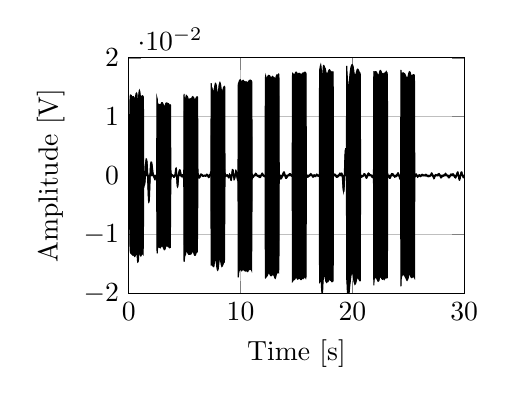
\begin{tikzpicture}

\begin{axis}[%
width=2.3in,
height=1.8in,
at={(0.758in,0.481in)},
xmin=0,
xmax=30,
xmajorgrids,
ymin=-0.02,
ymax=0.02,
ylabel={Amplitude [V]},
xlabel={Time [s]},
ymajorgrids,
axis background/.style={fill=white}
]
\addplot[fill=black,draw=black,forget plot] plot table[row sep=crcr]{%
2.08333333333333e-05	2.71797180175781e-05\\
0.0252733410493827	0.000192880630493164\\
0.0505258487654321	0.000219583511352539\\
0.0757783564814815	0.000324606895446777\\
0.101030864197531	0.0119782686233521\\
0.12628337191358	0.0132733583450317\\
0.15153587962963	0.0136597156524658\\
0.176788387345679	0.0136870145797729\\
0.202040895061728	0.0136398077011108\\
0.227293402777778	0.0136044025421143\\
0.252545910493827	0.0134916305541992\\
0.277798418209877	0.0134435892105103\\
0.303050925925926	0.0133676528930664\\
0.328303433641975	0.013298511505127\\
0.353555941358025	0.0132908821105957\\
0.378808449074074	0.0133390426635742\\
0.404060956790123	0.0133852958679199\\
0.429313464506173	0.0134091377258301\\
0.454565972222222	0.0132846832275391\\
0.479818479938272	0.0131728649139404\\
0.505070987654321	0.013127326965332\\
0.53032349537037	0.013005256652832\\
0.55557600308642	0.0130565166473389\\
0.580828510802469	0.0131419897079468\\
0.606081018518519	0.0132650136947632\\
0.631333526234568	0.0136377811431885\\
0.656586033950617	0.013906717300415\\
0.681838541666667	0.0139398574829102\\
0.707091049382716	0.014009952545166\\
0.732343557098765	0.0138951539993286\\
0.757596064814815	0.0131340026855469\\
0.782848572530864	0.0125246047973633\\
0.808101080246914	0.0120847225189209\\
0.833353587962963	0.0121047496795654\\
0.858606095679012	0.0126000642776489\\
0.883858603395062	0.0132580995559692\\
0.909111111111111	0.0139368772506714\\
0.934363618827161	0.0143285989761353\\
0.95961612654321	0.0144567489624023\\
0.984868634259259	0.0143048763275146\\
1.01012114197531	0.0140185356140137\\
1.03537364969136	0.0135726928710938\\
1.06062615740741	0.0131675004959106\\
1.08587866512346	0.0131186246871948\\
1.11113117283951	0.0132516622543335\\
1.13638368055556	0.0133669376373291\\
1.16163618827161	0.0134577751159668\\
1.18688869598765	0.013525128364563\\
1.2121412037037	0.0135258436203003\\
1.23739371141975	0.0135520696640015\\
1.2626462191358	0.0135167837142944\\
1.28789872685185	0.0133790969848633\\
1.3131512345679	0.0133394002914429\\
1.33840374228395	0.00212621688842773\\
1.36365625	0.000198721885681152\\
1.38890875771605	-0.000733494758605957\\
1.4141612654321	-0.00125908851623535\\
1.43941377314815	-0.00092923641204834\\
1.4646662808642	2.55107879638672e-05\\
1.48991878858025	0.00101137161254883\\
1.5151712962963	0.00201702117919922\\
1.54042380401235	0.00256431102752686\\
1.5656763117284	0.00282752513885498\\
1.59092881944444	0.00278055667877197\\
1.61618132716049	0.00261569023132324\\
1.64143383487654	0.00230515003204346\\
1.66668634259259	0.00142943859100342\\
1.69193885030864	0.000802040100097656\\
1.71719135802469	-0.000465273857116699\\
1.74244386574074	-0.00176858901977539\\
1.76769637345679	-0.00314795970916748\\
1.79294888117284	-0.00413775444030762\\
1.81820138888889	-0.00416898727416992\\
1.84345389660494	-0.00293600559234619\\
1.86870640432099	-0.00164687633514404\\
1.89395891203704	-0.000130534172058105\\
1.91921141975309	0.000895500183105469\\
1.94446392746914	0.00174665451049805\\
1.96971643518519	0.00211250782012939\\
1.99496894290123	0.00230598449707031\\
2.02022145061728	0.0022965669631958\\
2.04547395833333	0.00227689743041992\\
2.07072646604938	0.00209701061248779\\
2.09597897376543	0.00173783302307129\\
2.12123148148148	0.00134444236755371\\
2.14648398919753	0.000928759574890137\\
2.17173649691358	0.000492453575134277\\
2.19698900462963	0.000280857086181641\\
2.22224151234568	3.7074089050293e-05\\
2.24749402006173	-3.07559967041016e-05\\
2.27274652777778	-0.000232815742492676\\
2.29799903549383	-0.000373005867004395\\
2.32325154320988	-0.000491857528686523\\
2.34850405092593	-0.000524044036865234\\
2.37375655864198	-0.00048983097076416\\
2.39900906635802	-0.00031745433807373\\
2.42426157407407	-0.000228166580200195\\
2.44951408179012	-0.000116825103759766\\
2.47476658950617	-3.49283218383789e-05\\
2.50001909722222	-2.86102294921875e-06\\
2.52527160493827	0.0131807327270508\\
2.55052411265432	0.0129787921905518\\
2.57577662037037	0.0122307538986206\\
2.60102912808642	0.0119733810424805\\
2.62628163580247	0.0121581554412842\\
2.65153414351852	0.0121017694473267\\
2.67678665123457	0.0120164155960083\\
2.70203915895062	0.012006402015686\\
2.72729166666667	0.0119665861129761\\
2.75254417438272	0.0120497941970825\\
2.77779668209877	0.0120284557342529\\
2.80304918981481	0.0120289325714111\\
2.82830169753086	0.0119181871414185\\
2.85355420524691	0.0119922161102295\\
2.87880671296296	0.0121314525604248\\
2.90405922067901	0.0121816396713257\\
2.92931172839506	0.012296199798584\\
2.95456423611111	0.0123827457427979\\
2.97981674382716	0.0123804807662964\\
3.00506925154321	0.0123680830001831\\
3.03032175925926	0.0123096704483032\\
3.05557426697531	0.0122144222259521\\
3.08082677469136	0.0120468139648438\\
3.10607928240741	0.0120029449462891\\
3.13133179012346	0.0118519067764282\\
3.15658429783951	0.0116713047027588\\
3.18183680555556	0.0115656852722168\\
3.2070893132716	0.0115969181060791\\
3.23234182098765	0.0117167234420776\\
3.2575943287037	0.0118753910064697\\
3.28284683641975	0.0120331048965454\\
3.3080993441358	0.0122144222259521\\
3.33335185185185	0.0122911930084229\\
3.3586043595679	0.0123170614242554\\
3.38385686728395	0.0122699737548828\\
3.409109375	0.0123218297958374\\
3.43436188271605	0.01230788230896\\
3.4596143904321	0.0122936964035034\\
3.48486689814815	0.0122591257095337\\
3.5101194058642	0.0121793746948242\\
3.53537191358025	0.0122112035751343\\
3.5606244212963	0.012218713760376\\
3.58587692901235	0.0120950937271118\\
3.61112943672839	0.0120012760162354\\
3.63638194444444	0.0119942426681519\\
3.66163445216049	0.0119779109954834\\
3.68688695987654	0.0119713544845581\\
3.71213946759259	0.0120042562484741\\
3.73739197530864	0.0119483470916748\\
3.76264448302469	0.00140035152435303\\
3.78789699074074	0.000461459159851074\\
3.81314949845679	0.000228643417358398\\
3.83840200617284	0.000122308731079102\\
3.86365451388889	0.00018775463104248\\
3.88890702160494	0.000143051147460938\\
3.91415952932099	9.60826873779297e-05\\
3.93941203703704	3.83853912353516e-05\\
3.96466454475309	3.01599502563477e-05\\
3.98991705246914	-4.05311584472656e-06\\
4.01516956018518	-7.51018524169922e-05\\
4.04042206790123	-0.000198602676391602\\
4.06567457561728	-0.000174880027770996\\
4.09092708333333	-0.000170588493347168\\
4.11617959104938	-7.84397125244141e-05\\
4.14143209876543	0.000242471694946289\\
4.16668460648148	0.00061953067779541\\
4.19193711419753	0.00105559825897217\\
4.21718962191358	0.00124335289001465\\
4.24244212962963	0.00129139423370361\\
4.26769463734568	0.00111246109008789\\
4.29294714506173	0.000468969345092773\\
4.31819965277778	-0.000456333160400391\\
4.34345216049383	-0.00124490261077881\\
4.36870466820988	-0.00180208683013916\\
4.39395717592593	-0.00133395195007324\\
4.41920968364198	-0.000530719757080078\\
4.44446219135802	-4.05311584472656e-05\\
4.46971469907407	0.000434398651123047\\
4.49496720679012	0.000670433044433594\\
4.52021971450617	0.000893712043762207\\
4.54547222222222	0.000962257385253906\\
4.57072472993827	0.000990629196166992\\
4.59597723765432	0.000925421714782715\\
4.62122974537037	0.000837922096252441\\
4.64648225308642	0.00060117244720459\\
4.67173476080247	0.00031888484954834\\
4.69698726851852	1.08480453491211e-05\\
4.72223977623457	-6.46114349365234e-05\\
4.74749228395062	4.62532043457031e-05\\
4.77274479166667	7.72476196289063e-05\\
4.79799729938272	0.000130534172058105\\
4.82324980709877	0.000133872032165527\\
4.84850231481482	2.68220901489258e-05\\
4.87375482253086	-0.000166893005371094\\
4.89900733024691	-0.00031590461730957\\
4.92425983796296	-0.000426411628723145\\
4.94951234567901	0.0138906240463257\\
4.97476485339506	0.0127924680709839\\
5.00001736111111	0.0127823352813721\\
5.02526986882716	0.0127456188201904\\
5.05052237654321	0.012772798538208\\
5.07577488425926	0.0129667520523071\\
5.10102739197531	0.0132062435150146\\
5.12627989969136	0.0134183168411255\\
5.15153240740741	0.0136046409606934\\
5.17678491512346	0.0135563611984253\\
5.20203742283951	0.0135209560394287\\
5.22728993055556	0.0134320259094238\\
5.2525424382716	0.0134093761444092\\
5.27779494598765	0.0132806301116943\\
5.3030474537037	0.0131157636642456\\
5.32829996141975	0.0129809379577637\\
5.3535524691358	0.0129413604736328\\
5.37880497685185	0.0128811597824097\\
5.4040574845679	0.0128850936889648\\
5.42930999228395	0.012834906578064\\
5.4545625	0.0129283666610718\\
5.47981500771605	0.0130480527877808\\
5.5050675154321	0.0130259990692139\\
5.53032002314815	0.0129679441452026\\
5.5555725308642	0.0129989385604858\\
5.58082503858025	0.0130027532577515\\
5.6060775462963	0.0131098031997681\\
5.63133005401235	0.0131270885467529\\
5.65658256172839	0.0132246017456055\\
5.68183506944444	0.0133410692214966\\
5.70708757716049	0.0133851766586304\\
5.73234008487654	0.0134118795394897\\
5.75759259259259	0.0132910013198853\\
5.78284510030864	0.0132763385772705\\
5.80809760802469	0.0132464170455933\\
5.83335011574074	0.0131045579910278\\
5.85860262345679	0.0130085945129395\\
5.88385513117284	0.012847900390625\\
5.90910763888889	0.0127744674682617\\
5.93436014660494	0.0128093957901001\\
5.95961265432099	0.0128616094589233\\
5.98486516203704	0.0129320621490479\\
6.01011766975309	0.0131421089172363\\
6.03537017746914	0.0131816864013672\\
6.06062268518518	0.0133038759231567\\
6.08587519290123	0.0133326053619385\\
6.11112770061728	0.0133798122406006\\
6.13638020833333	0.0133734941482544\\
6.16163271604938	0.0133055448532104\\
6.18688522376543	0.00129294395446777\\
6.21213773148148	0.000391721725463867\\
6.23739023919753	0.000118851661682129\\
6.26264274691358	-6.7591667175293e-05\\
6.28789525462963	-0.00014650821685791\\
6.31314776234568	-0.000262737274169922\\
6.33840027006173	-0.000207424163818359\\
6.36365277777778	-0.000160098075866699\\
6.38890528549383	-3.62396240234375e-05\\
6.41415779320988	0.000113129615783691\\
6.43941030092593	0.000204920768737793\\
6.46466280864198	0.000273823738098145\\
6.48991531635802	0.000244855880737305\\
6.51516782407407	0.000198602676391602\\
6.54042033179012	0.000207901000976563\\
6.56567283950617	0.000176548957824707\\
6.59092534722222	9.56058502197266e-05\\
6.61617785493827	1.53779983520508e-05\\
6.64143036265432	-4.20808792114258e-05\\
6.66668287037037	-2.02655792236328e-06\\
6.69193537808642	-1.70469284057617e-05\\
6.71718788580247	3.08752059936523e-05\\
6.74244039351852	4.80413436889648e-05\\
6.76769290123457	5.51939010620117e-05\\
6.79294540895062	6.13927841186523e-05\\
6.81819791666667	1.4185905456543e-05\\
6.84345042438272	2.51531600952148e-05\\
6.86870293209877	-3.33786010742188e-06\\
6.89395543981481	-1.58548355102539e-05\\
6.91920794753086	0.000109314918518066\\
6.94446045524691	0.00016486644744873\\
6.96971296296296	0.000245809555053711\\
6.99496547067901	0.000245332717895508\\
7.02021797839506	0.000184535980224609\\
7.04547048611111	0.000141501426696777\\
7.07072299382716	0.000122666358947754\\
7.09597550154321	-4.24385070800781e-05\\
7.12122800925926	-0.000117182731628418\\
7.14648051697531	-0.000206112861633301\\
7.17173302469136	-0.000195622444152832\\
7.19698553240741	-4.50611114501953e-05\\
7.22223804012346	2.41994857788086e-05\\
7.24749054783951	0.000180721282958984\\
7.27274305555556	0.000224471092224121\\
7.2979955632716	0.000301599502563477\\
7.32324807098765	0.000630378723144531\\
7.3485005787037	0.000650882720947266\\
7.37375308641975	0.0156896114349365\\
7.3990055941358	0.0150365829467773\\
7.42425810185185	0.0149332284927368\\
7.4495106095679	0.0148735046386719\\
7.47476311728395	0.0145994424819946\\
7.500015625	0.0142728090286255\\
7.52526813271605	0.0143123865127563\\
7.5505206404321	0.0141353607177734\\
7.57577314814815	0.0140994787216187\\
7.6010256558642	0.0140562057495117\\
7.62627816358025	0.0144972801208496\\
7.6515306712963	0.0147725343704224\\
7.67678317901235	0.0148419141769409\\
7.70203568672839	0.0152887105941772\\
7.72728819444444	0.015468955039978\\
7.75254070216049	0.0156747102737427\\
7.77779320987654	0.0156437158584595\\
7.80304571759259	0.0155001878738403\\
7.82829822530864	0.0153249502182007\\
7.85355073302469	0.0149215459823608\\
7.87880324074074	0.0144649744033813\\
7.90405574845679	0.0139764547348022\\
7.92930825617284	0.0136035680770874\\
7.95456076388889	0.0135245323181152\\
7.97981327160494	0.0136982202529907\\
8.00506577932099	0.0140670537948608\\
8.03031828703704	0.0143532752990723\\
8.05557079475309	0.0147926807403564\\
8.08082330246914	0.0153083801269531\\
8.10607581018519	0.015499472618103\\
8.13132831790123	0.0156772136688232\\
8.15658082561728	0.0157968997955322\\
8.18183333333333	0.0156925916671753\\
8.20708584104938	0.0154823064804077\\
8.23233834876543	0.0152593851089478\\
8.25759085648148	0.014828085899353\\
8.28284336419753	0.0144996643066406\\
8.30809587191358	0.0143203735351563\\
8.33334837962963	0.0142027139663696\\
8.35860088734568	0.0142422914505005\\
8.38385339506173	0.0143022537231445\\
8.40910590277778	0.01442551612854\\
8.43435841049383	0.0146499872207642\\
8.45961091820988	0.0148167610168457\\
8.48486342592593	0.0149878263473511\\
8.51011593364198	0.0150655508041382\\
8.53536844135802	0.0150963068008423\\
8.56062094907407	0.0151380300521851\\
8.58587345679012	0.0150313377380371\\
8.61112596450617	0.000926375389099121\\
8.63637847222222	0.000237107276916504\\
8.66163097993827	1.70469284057617e-05\\
8.68688348765432	-1.04904174804688e-05\\
8.71213599537037	7.79628753662109e-05\\
8.73738850308642	8.10623168945313e-05\\
8.76264101080247	9.01222229003906e-05\\
8.78789351851852	0.000140666961669922\\
8.81314602623457	0.000134706497192383\\
8.83839853395062	6.63995742797852e-05\\
8.86365104166667	1.8000602722168e-05\\
8.88890354938272	-0.000120162963867188\\
8.91415605709877	-0.00020444393157959\\
8.93940856481481	-0.000177621841430664\\
8.96466107253086	-6.72340393066406e-05\\
8.98991358024691	7.18832015991211e-05\\
9.01516608796296	0.000251293182373047\\
9.04041859567901	0.000190377235412598\\
9.06567110339506	0.000151991844177246\\
9.09092361111111	-7.84397125244141e-05\\
9.11617611882716	-0.000372886657714844\\
9.14142862654321	-0.000590682029724121\\
9.16668113425926	-0.00061953067779541\\
9.19193364197531	-0.000303745269775391\\
9.21718614969136	0.00022578239440918\\
9.24243865740741	0.000708937644958496\\
9.26769116512346	0.00102901458740234\\
9.29294367283951	0.00101268291473389\\
9.31819618055556	0.000956416130065918\\
9.34344868827161	0.000914931297302246\\
9.36870119598765	0.000367522239685059\\
9.3939537037037	2.45571136474609e-05\\
9.41920621141975	-0.000287413597106934\\
9.4444587191358	-0.000396251678466797\\
9.46971122685185	-0.000282764434814453\\
9.4949637345679	-5.55515289306641e-05\\
9.52021624228395	0.000377655029296875\\
9.54546875	0.000602841377258301\\
9.57072125771605	0.000919580459594727\\
9.5959737654321	0.000896334648132324\\
9.62122627314815	0.000671863555908203\\
9.6464787808642	0.000562429428100586\\
9.67173128858025	0.000257372856140137\\
9.6969837962963	-0.000269532203674316\\
9.72223630401235	-0.000421762466430664\\
9.7474888117284	-0.000730991363525391\\
9.77274131944444	-0.000650405883789063\\
9.79799382716049	0.0154277086257935\\
9.82324633487654	0.0156807899475098\\
9.84849884259259	0.0157598257064819\\
9.87375135030864	0.0159609317779541\\
9.89900385802469	0.0161114931106567\\
9.92425636574074	0.0161769390106201\\
9.94950887345679	0.0162290334701538\\
9.97476138117284	0.0162595510482788\\
10.0000138888889	0.0160911083221436\\
10.0252663966049	0.0160559415817261\\
10.050518904321	0.0159459114074707\\
10.075771412037	0.0158594846725464\\
10.1010239197531	0.0158390998840332\\
10.1262764274691	0.0159010887145996\\
10.1515289351852	0.0160681009292603\\
10.1767814429012	0.0160746574401855\\
10.2020339506173	0.0161263942718506\\
10.2272864583333	0.0161761045455933\\
10.2525389660494	0.0161302089691162\\
10.2777914737654	0.0160362720489502\\
10.3030439814815	0.0160095691680908\\
10.3282964891975	0.0159236192703247\\
10.3535489969136	0.0159534215927124\\
10.3788015046296	0.0158895254135132\\
10.4040540123457	0.0158728361129761\\
10.4293065200617	0.0158777236938477\\
10.4545590277778	0.0158460140228271\\
10.4798115354938	0.015931248664856\\
10.5050640432099	0.0159186124801636\\
10.5303165509259	0.0159024000167847\\
10.555569058642	0.0158482789993286\\
10.580821566358	0.015781044960022\\
10.6060740740741	0.0157147645950317\\
10.6313265817901	0.0157208442687988\\
10.6565790895062	0.0157356262207031\\
10.6818315972222	0.0159025192260742\\
10.7070841049383	0.0159567594528198\\
10.7323366126543	0.0160346031188965\\
10.7575891203704	0.0160861015319824\\
10.7828416280864	0.0160651206970215\\
10.8080941358025	0.0160901546478271\\
10.8333466435185	0.016063928604126\\
10.8585991512346	0.0161927938461304\\
10.8838516589506	0.0161173343658447\\
10.9091041666667	0.0161306858062744\\
10.9343566743827	0.0161368846893311\\
10.9596091820988	0.0161256790161133\\
10.9848616898148	0.0159846544265747\\
11.0101141975309	0.0159024000167847\\
11.0353667052469	0.000484466552734375\\
11.060619212963	-4.20808792114258e-05\\
11.085871720679	-0.000198245048522949\\
11.1111242283951	-0.000219464302062988\\
11.1363767361111	-0.000158071517944336\\
11.1616292438272	-0.000123023986816406\\
11.1868817515432	-8.08238983154297e-05\\
11.2121342592593	6.79492950439453e-05\\
11.2373867669753	0.000106930732727051\\
11.2626392746914	0.000181078910827637\\
11.2878917824074	0.000208735466003418\\
11.3131442901235	0.000313282012939453\\
11.3383967978395	0.000393390655517578\\
11.3636493055556	0.000383138656616211\\
11.3889018132716	0.000328779220581055\\
11.4141543209877	0.000310063362121582\\
11.4394068287037	0.000229954719543457\\
11.4646593364198	0.000151157379150391\\
11.4899118441358	5.84125518798828e-05\\
11.5151643518519	3.34978103637695e-05\\
11.5404168595679	-4.55379486083984e-05\\
11.565669367284	-5.91278076171875e-05\\
11.590921875	-7.34329223632813e-05\\
11.6161743827161	-0.000102996826171875\\
11.6414268904321	-0.000104308128356934\\
11.6666793981481	-0.000190258026123047\\
11.6919319058642	-0.000185608863830566\\
11.7171844135802	-0.000193119049072266\\
11.7424369212963	-0.000184893608093262\\
11.7676894290123	-0.000196099281311035\\
11.7929419367284	-0.000140070915222168\\
11.8181944444444	1.53779983520508e-05\\
11.8434469521605	0.000145673751831055\\
11.8686994598765	0.000226259231567383\\
11.8939519675926	0.000336289405822754\\
11.9192044753086	0.000395894050598145\\
11.9444569830247	0.000421047210693359\\
11.9697094907407	0.000374794006347656\\
11.9949619984568	0.000291228294372559\\
12.0202145061728	0.000190615653991699\\
12.0454670138889	0.000115513801574707\\
12.0707195216049	3.0517578125e-05\\
12.095972029321	-2.41994857788086e-05\\
12.121224537037	-8.46385955810547e-05\\
12.1464770447531	-7.55786895751953e-05\\
12.1717295524691	-9.41753387451172e-05\\
12.1969820601852	-5.48362731933594e-06\\
12.2222345679012	0.0165671110153198\\
12.2474870756173	0.0168999433517456\\
12.2727395833333	0.0166717767715454\\
12.2979920910494	0.0165742635726929\\
12.3232445987654	0.0165170431137085\\
12.3484971064815	0.0165308713912964\\
12.3737496141975	0.016585111618042\\
12.3990021219136	0.0166263580322266\\
12.4242546296296	0.0167803764343262\\
12.4495071373457	0.0168399810791016\\
12.4747596450617	0.0169746875762939\\
12.5000121527778	0.0169860124588013\\
12.5252646604938	0.0170214176177979\\
12.5505171682099	0.0169990062713623\\
12.5757696759259	0.0169893503189087\\
12.601022183642	0.0169556140899658\\
12.626274691358	0.0168999433517456\\
12.6515271990741	0.0167281627655029\\
12.6767797067901	0.0166318416595459\\
12.7020322145062	0.0165399312973022\\
12.7272847222222	0.0165116786956787\\
12.7525372299383	0.0165554285049438\\
12.7777897376543	0.01661217212677\\
12.8030422453704	0.0167293548583984\\
12.8282947530864	0.0167727470397949\\
12.8535472608025	0.0168174505233765\\
12.8787997685185	0.0166926383972168\\
12.9040522762346	0.0167468786239624\\
12.9293047839506	0.0166680812835693\\
12.9545572916667	0.016689658164978\\
12.9798097993827	0.0166734457015991\\
13.0050623070988	0.0166347026824951\\
13.0303148148148	0.016505241394043\\
13.0555673225309	0.0163514614105225\\
13.0808198302469	0.0162187814712524\\
13.106072337963	0.0161361694335938\\
13.131324845679	0.0162808895111084\\
13.1565773533951	0.0165536403656006\\
13.1818298611111	0.0167999267578125\\
13.2070823688272	0.0169224739074707\\
13.2323348765432	0.017076849937439\\
13.2575873842593	0.017071008682251\\
13.2828398919753	0.0170369148254395\\
13.3080923996914	0.0170255899429321\\
13.3333449074074	0.0170601606369019\\
13.3585974151235	0.0171662569046021\\
13.3838499228395	0.0171995162963867\\
13.4091024305556	0.017237663269043\\
13.4343549382716	0.0171002149581909\\
13.4596074459877	0.00082862377166748\\
13.4848599537037	0.000102758407592773\\
13.5101124614198	-9.918212890625e-05\\
13.5353649691358	-0.000249147415161133\\
13.5606174768519	-0.000396728515625\\
13.5858699845679	-0.000394225120544434\\
13.611122492284	-0.00046849250793457\\
13.636375	-0.000432133674621582\\
13.6616275077161	-0.000347495079040527\\
13.6868800154321	-0.000221014022827148\\
13.7121325231481	-9.14335250854492e-05\\
13.7373850308642	-1.00135803222656e-05\\
13.7626375385802	0.000199437141418457\\
13.7878900462963	0.00036931037902832\\
13.8131425540123	0.000469803810119629\\
13.8383950617284	0.000552892684936523\\
13.8636475694444	0.000609636306762695\\
13.8889000771605	0.000621199607849121\\
13.9141525848765	0.000609278678894043\\
13.9394050925926	0.000482797622680664\\
13.9646576003086	0.000282883644104004\\
13.9899101080247	7.42673873901367e-05\\
14.0151626157407	-0.000166416168212891\\
14.0404151234568	-0.000336170196533203\\
14.0656676311728	-0.000344991683959961\\
14.0909201388889	-0.000310778617858887\\
14.1161726466049	-0.000333666801452637\\
14.141425154321	-0.000180602073669434\\
14.166677662037	-0.00015723705291748\\
14.1919301697531	-6.13927841186523e-05\\
14.2171826774691	-1.87158584594727e-05\\
14.2424351851852	4.25577163696289e-05\\
14.2676876929012	0.000150203704833984\\
14.2929402006173	0.000175714492797852\\
14.3181927083333	0.000205278396606445\\
14.3434452160494	0.000236988067626953\\
14.3686977237654	0.000314712524414063\\
14.3939502314815	0.000324130058288574\\
14.4192027391975	0.000327944755554199\\
14.4444552469136	0.000308752059936523\\
14.4697077546296	0.00026547908782959\\
14.4949602623457	0.000200629234313965\\
14.5202127700617	0.000146389007568359\\
14.5454652777778	6.92605972290039e-05\\
14.5707177854938	7.15255737304688e-06\\
14.5959702932099	3.00407409667969e-05\\
14.6212228009259	1.62124633789063e-05\\
14.646475308642	0.0169292688369751\\
14.671727816358	0.0173319578170776\\
14.6969803240741	0.0172630548477173\\
14.7222328317901	0.0172011852264404\\
14.7474853395062	0.0171821117401123\\
14.7727378472222	0.0171287059783936\\
14.7979903549383	0.0171319246292114\\
14.8232428626543	0.0171495676040649\\
14.8484953703704	0.0171682834625244\\
14.8737478780864	0.0171934366226196\\
14.8990003858025	0.0174195766448975\\
14.9242528935185	0.0175316333770752\\
14.9495054012346	0.0175597667694092\\
14.9747579089506	0.0175731182098389\\
15.0000104166667	0.0175539255142212\\
15.0252629243827	0.0175000429153442\\
15.0505154320988	0.0173577070236206\\
15.0757679398148	0.0172542333602905\\
15.1010204475309	0.0171407461166382\\
15.1262729552469	0.0171658992767334\\
15.151525462963	0.0172443389892578\\
15.176777970679	0.0172475576400757\\
15.2020304783951	0.0173439979553223\\
15.2272829861111	0.0173681974411011\\
15.2525354938272	0.0173213481903076\\
15.2777880015432	0.0173455476760864\\
15.3030405092593	0.0173231363296509\\
15.3282930169753	0.0172563791275024\\
15.3535455246914	0.017225980758667\\
15.3787980324074	0.0171550512313843\\
15.4040505401235	0.0170636177062988\\
15.4293030478395	0.0170685052871704\\
15.4545555555556	0.0171319246292114\\
15.4798080632716	0.0172151327133179\\
15.5050605709877	0.0172789096832275\\
15.5303130787037	0.0173686742782593\\
15.5555655864198	0.0173188447952271\\
15.5808180941358	0.0173131227493286\\
15.6060706018519	0.0173306465148926\\
15.6313231095679	0.017390251159668\\
15.656575617284	0.0174404382705688\\
15.681828125	0.0174127817153931\\
15.7070806327161	0.0175391435623169\\
15.7323331404321	0.0175487995147705\\
15.7575856481481	0.0175501108169556\\
15.7828381558642	0.0175542831420898\\
15.8080906635802	0.0174723863601685\\
15.8333431712963	0.0174212455749512\\
15.8585956790123	0.0172785520553589\\
15.8838481867284	0.000405669212341309\\
15.9091006944444	8.47578048706055e-05\\
15.9343532021605	-6.92605972290039e-05\\
15.9596057098765	-2.07424163818359e-05\\
15.9848582175926	-0.000122547149658203\\
16.0101107253086	-0.00012052059173584\\
16.0353632330247	-0.000148892402648926\\
16.0606157407407	-0.000107645988464355\\
16.0858682484568	-3.40938568115234e-05\\
16.1111207561728	-4.16040420532227e-05\\
16.1363732638889	8.47578048706055e-05\\
16.1616257716049	0.000107288360595703\\
16.186878279321	0.000143051147460938\\
16.212130787037	0.000160574913024902\\
16.2373832947531	0.000275850296020508\\
16.2626358024691	0.000192046165466309\\
16.2878883101852	0.000250697135925293\\
16.3131408179012	0.000265836715698242\\
16.3383933256173	0.000269889831542969\\
16.3636458333333	0.000122189521789551\\
16.3888983410494	0.00011444091796875\\
16.4141508487654	4.45842742919922e-05\\
16.4394033564815	-3.42130661010742e-05\\
16.4646558641975	-0.000105977058410645\\
16.4899083719136	-1.00135803222656e-05\\
16.5151608796296	-0.0001068115234375\\
16.5404133873457	6.79492950439453e-06\\
16.5656658950617	8.84532928466797e-05\\
16.5909184027778	6.46114349365234e-05\\
16.6161709104938	0.000111937522888184\\
16.6414234182099	6.18696212768555e-05\\
16.6666759259259	7.46250152587891e-05\\
16.691928433642	-3.75509262084961e-05\\
16.717180941358	2.86102294921875e-06\\
16.7424334490741	6.50882720947266e-05\\
16.7676859567901	0.000104427337646484\\
16.7929384645062	0.000123023986816406\\
16.8181909722222	0.000252127647399902\\
16.8434434799383	0.000231504440307617\\
16.8686959876543	0.000136375427246094\\
16.8939484953704	7.71284103393555e-05\\
16.9192010030864	8.46385955810547e-05\\
16.9444535108025	9.02414321899414e-05\\
16.9697060185185	8.14199447631836e-05\\
16.9949585262346	0.000124812126159668\\
17.0202110339506	0.000126481056213379\\
17.0454635416667	5.80549240112305e-05\\
17.0707160493827	0.0179164409637451\\
17.0959685570988	0.0180661678314209\\
17.1212210648148	0.0184476375579834\\
17.1464735725309	0.0186307430267334\\
17.1717260802469	0.0187876224517822\\
17.196978587963	0.0185372829437256\\
17.222231095679	0.0179513692855835\\
17.2474836033951	0.0168821811676025\\
17.2727361111111	0.0159904956817627\\
17.2979886188272	0.0154684782028198\\
17.3232411265432	0.0159759521484375\\
17.3484936342593	0.0165970325469971\\
17.3737461419753	0.0177416801452637\\
17.3989986496914	0.0184311866760254\\
17.4242511574074	0.0186929702758789\\
17.4495036651235	0.0186983346939087\\
17.4747561728395	0.0186036825180054\\
17.5000086805556	0.0184463262557983\\
17.5252611882716	0.0182918310165405\\
17.5505136959877	0.0182555913925171\\
17.5757662037037	0.0181587934494019\\
17.6010187114198	0.0178960561752319\\
17.6262712191358	0.0177195072174072\\
17.6515237268519	0.0174219608306885\\
17.6767762345679	0.0173271894454956\\
17.702028742284	0.0173096656799316\\
17.72728125	0.0173647403717041\\
17.7525337577161	0.0173664093017578\\
17.7777862654321	0.0174031257629395\\
17.8030387731481	0.0174136161804199\\
17.8282912808642	0.0174782276153564\\
17.8535437885803	0.0175955295562744\\
17.8787962962963	0.0177769660949707\\
17.9040488040123	0.0178405046463013\\
17.9293013117284	0.0179694890975952\\
17.9545538194444	0.0179864168167114\\
17.9798063271605	0.0179113149642944\\
18.0050588348765	0.0178525447845459\\
18.0303113425926	0.0176674127578735\\
18.0555638503086	0.0176661014556885\\
18.0808163580247	0.0176839828491211\\
18.1060688657407	0.0176535844802856\\
18.1313213734568	0.0175237655639648\\
18.1565738811728	0.017460823059082\\
18.1818263888889	0.0174012184143066\\
18.2070788966049	0.0174828767776489\\
18.232331404321	0.0174508094787598\\
18.257583912037	0.017616868019104\\
18.2828364197531	0.0175806283950806\\
18.3080889274691	0.000448226928710938\\
18.3333414351852	0.00021660327911377\\
18.3585939429012	0.00025629997253418\\
18.3838464506173	0.000190377235412598\\
18.4090989583333	0.000196099281311035\\
18.4343514660494	0.000238776206970215\\
18.4596039737654	0.000233769416809082\\
18.4848564814815	0.000162005424499512\\
18.5101089891975	0.000110983848571777\\
18.5353614969136	-2.21729278564453e-05\\
18.5606140046296	-2.96831130981445e-05\\
18.5858665123457	-9.93013381958008e-05\\
18.6111190200617	-0.000138998031616211\\
18.6363715277778	-0.000132203102111816\\
18.6616240354938	-0.000133991241455078\\
18.6868765432099	-0.000164389610290527\\
18.7121290509259	-8.96453857421875e-05\\
18.737381558642	-5.50746917724609e-05\\
18.762634066358	7.43865966796875e-05\\
18.7878865740741	0.000127196311950684\\
18.8131390817901	0.000230312347412109\\
18.8383915895062	0.000272393226623535\\
18.8636440972222	0.000393390655517578\\
18.8888966049383	0.000400662422180176\\
18.9141491126543	0.000297904014587402\\
18.9394016203704	0.000269889831542969\\
18.9646541280864	0.000294923782348633\\
18.9899066358025	0.000373482704162598\\
19.0151591435185	0.000348806381225586\\
19.0404116512346	0.000412225723266602\\
19.0656641589506	0.000396013259887695\\
19.0909166666667	0.000279664993286133\\
19.1161691743827	-5.59091567993164e-05\\
19.1414216820988	-0.000618696212768555\\
19.1666741898148	-0.00137102603912354\\
19.1919266975309	-0.00211083889007568\\
19.2171792052469	-0.00251805782318115\\
19.242431712963	-0.00203609466552734\\
19.267684220679	-0.000851988792419434\\
19.2929367283951	0.000642061233520508\\
19.3181892361111	0.00228226184844971\\
19.3434417438272	0.00357353687286377\\
19.3686942515432	0.00432217121124268\\
19.3939467592593	0.00450289249420166\\
19.4191992669753	0.00446105003356934\\
19.4444517746914	0.00392818450927734\\
19.4697042824074	0.00306880474090576\\
19.4949567901235	0.0186182260513306\\
19.5202092978395	0.0174990892410278\\
19.5454618055556	0.0167573690414429\\
19.5707143132716	0.0156563520431519\\
19.5959668209877	0.0149348974227905\\
19.6212193287037	0.01460862159729\\
19.6464718364198	0.014657735824585\\
19.6717243441358	0.0149654150009155\\
19.6969768518519	0.0154080390930176\\
19.7222293595679	0.0158551931381226\\
19.747481867284	0.0163990259170532\\
19.772734375	0.0168666839599609\\
19.797986882716	0.0174103975296021\\
19.8232393904321	0.0177158117294312\\
19.8484918981482	0.0181130170822144\\
19.8737444058642	0.0183916091918945\\
19.8989969135802	0.0185835361480713\\
19.9242494212963	0.0186495780944824\\
19.9495019290123	0.0187809467315674\\
19.9747544367284	0.0187575817108154\\
20.0000069444444	0.0188125371932983\\
20.0252594521605	0.0186846256256104\\
20.0505119598765	0.0186182260513306\\
20.0757644675926	0.0184367895126343\\
20.1010169753086	0.0180631875991821\\
20.1262694830247	0.017815113067627\\
20.1515219907407	0.01743483543396\\
20.1767744984568	0.017147421836853\\
20.2020270061728	0.0169249773025513\\
20.2272795138889	0.0168775320053101\\
20.2525320216049	0.0168746709823608\\
20.277784529321	0.0169830322265625\\
20.303037037037	0.0171991586685181\\
20.3282895447531	0.0172855854034424\\
20.3535420524691	0.0174849033355713\\
20.3787945601852	0.0177160501480103\\
20.4040470679012	0.0177884101867676\\
20.4292995756173	0.0180319547653198\\
20.4545520833333	0.0180799961090088\\
20.4798045910494	0.018064022064209\\
20.5050570987654	0.0180245637893677\\
20.5303096064815	0.0179439783096313\\
20.5555621141975	0.0178685188293457\\
20.5808146219136	0.0177570581436157\\
20.6060671296296	0.0175374746322632\\
20.6313196373457	0.0175430774688721\\
20.6565721450617	0.017493724822998\\
20.6818246527778	0.0174106359481812\\
20.7070771604938	0.0171592235565186\\
20.7323296682099	0.000139713287353516\\
20.7575821759259	-3.37362289428711e-05\\
20.782834683642	-0.000109195709228516\\
20.808087191358	-9.17911529541016e-05\\
20.8333396990741	-7.46250152587891e-05\\
20.8585922067901	-4.33921813964844e-05\\
20.8838447145062	-7.25984573364258e-05\\
20.9090972222222	-8.38041305541992e-05\\
20.9343497299383	-2.80141830444336e-05\\
20.9596022376543	3.58819961547852e-05\\
20.9848547453704	4.8518180847168e-05\\
21.0101072530864	0.000126957893371582\\
21.0353597608025	0.000322937965393066\\
21.0606122685185	0.000291347503662109\\
21.0858647762346	0.00032806396484375\\
21.1111172839506	0.000323891639709473\\
21.1363697916667	0.000241279602050781\\
21.1616222993827	0.00010228157043457\\
21.1868748070988	-1.13248825073242e-05\\
21.2121273148148	-0.000200152397155762\\
21.2373798225309	-0.000227689743041992\\
21.2626323302469	-0.000326991081237793\\
21.287884837963	-0.00032341480255127\\
21.313137345679	-0.000106692314147949\\
21.3383898533951	1.76429748535156e-05\\
21.3636423611111	0.00022125244140625\\
21.3888948688272	0.000350832939147949\\
21.4141473765432	0.000402212142944336\\
21.4393998842593	0.000428199768066406\\
21.4646523919753	0.000411510467529297\\
21.4899048996914	0.000369668006896973\\
21.5151574074074	0.000343918800354004\\
21.5404099151235	0.000272989273071289\\
21.5656624228395	0.000220298767089844\\
21.5909149305556	0.000177383422851563\\
21.6161674382716	0.000154852867126465\\
21.6414199459877	0.000129818916320801\\
21.6666724537037	0.000105977058410645\\
21.6919249614198	0.000100135803222656\\
21.7171774691358	-1.95503234863281e-05\\
21.7424299768519	-5.340576171875e-05\\
21.7676824845679	-0.000153064727783203\\
21.792934992284	-0.000183582305908203\\
21.8181875	-0.000210165977478027\\
21.8434400077161	-0.000201106071472168\\
21.8686925154321	-0.000120639801025391\\
21.8939450231481	-4.49419021606445e-05\\
21.9191975308642	0.0177475214004517\\
21.9444500385803	0.0173670053482056\\
21.9697025462963	0.0173903703689575\\
21.9949550540123	0.0174099206924438\\
22.0202075617284	0.0175341367721558\\
22.0454600694444	0.0176265239715576\\
22.0707125771605	0.0176255702972412\\
22.0959650848765	0.0176335573196411\\
22.1212175925926	0.0175776481628418\\
22.1464701003086	0.0175797939300537\\
22.1717226080247	0.0175366401672363\\
22.1969751157407	0.0173623561859131\\
22.2222276234568	0.017267107963562\\
22.2474801311728	0.0171732902526855\\
22.2727326388889	0.0169675350189209\\
22.2979851466049	0.0169329643249512\\
22.323237654321	0.0168830156326294\\
22.348490162037	0.0169788599014282\\
22.3737426697531	0.0170691013336182\\
22.3989951774691	0.0172792673110962\\
22.4242476851852	0.0174456834793091\\
22.4495001929012	0.0176714658737183\\
22.4747527006173	0.0178101062774658\\
22.5000052083333	0.0178617238998413\\
22.5252577160494	0.0178629159927368\\
22.5505102237654	0.0177403688430786\\
22.5757627314815	0.017638087272644\\
22.6010152391975	0.017555832862854\\
22.6262677469136	0.0173798799514771\\
22.6515202546296	0.0172560214996338\\
22.6767727623457	0.01722252368927\\
22.7020252700617	0.0172896385192871\\
22.7272777777778	0.0172810554504395\\
22.7525302854938	0.0172203779220581\\
22.7777827932099	0.0172380208969116\\
22.8030353009259	0.0172601938247681\\
22.828287808642	0.0173335075378418\\
22.853540316358	0.0172879695892334\\
22.8787928240741	0.0173248052597046\\
22.9040453317901	0.0173823833465576\\
22.9292978395062	0.0174615383148193\\
22.9545503472222	0.0174990892410278\\
22.9798028549383	0.0174890756607056\\
23.0050553626543	0.0175430774688721\\
23.0303078703704	0.0176382064819336\\
23.0555603780864	0.0175291299819946\\
23.0808128858025	0.0175257921218872\\
23.1060653935185	0.0174691677093506\\
23.1313179012346	0.0169287919998169\\
23.1565704089506	0.000443935394287109\\
23.1818229166667	0.00018155574798584\\
23.2070754243827	-8.70227813720703e-06\\
23.2323279320988	-7.49826431274414e-05\\
23.2575804398148	-9.97781753540039e-05\\
23.2828329475309	-0.000157356262207031\\
23.3080854552469	-0.000261664390563965\\
23.333337962963	-0.000339508056640625\\
23.358590470679	-0.000370383262634277\\
23.3838429783951	-0.000281095504760742\\
23.4090954861111	-0.000164031982421875\\
23.4343479938272	-6.07967376708984e-05\\
23.4596005015432	0.000153064727783203\\
23.4848530092593	0.000249981880187988\\
23.5101055169753	0.000330924987792969\\
23.5353580246914	0.00034642219543457\\
23.5606105324074	0.000332117080688477\\
23.5858630401235	0.000333070755004883\\
23.6111155478395	0.000329732894897461\\
23.6363680555556	0.000268697738647461\\
23.6616205632716	0.000220298767089844\\
23.6868730709877	0.000146865844726563\\
23.7121255787037	3.57627868652344e-07\\
23.7373780864198	-1.20401382446289e-05\\
23.7626305941358	-7.67707824707031e-05\\
23.7878831018519	-0.000118017196655273\\
23.8131356095679	-0.000118374824523926\\
23.838388117284	-7.87973403930664e-05\\
23.863640625	-7.17639923095703e-05\\
23.888893132716	-0.000100851058959961\\
23.9141456404321	-3.96966934204102e-05\\
23.9393981481482	9.97781753540039e-05\\
23.9646506558642	0.000128030776977539\\
23.9899031635802	0.000224113464355469\\
24.0151556712963	0.000260353088378906\\
24.0404081790123	0.000397562980651855\\
24.0656606867284	0.000442743301391602\\
24.0909131944444	0.00046694278717041\\
24.1161657021605	0.000429272651672363\\
24.1414182098765	0.00032508373260498\\
24.1666707175926	0.000194549560546875\\
24.1919232253086	-6.22272491455078e-05\\
24.2171757330247	-0.000203251838684082\\
24.2424282407407	-0.000442743301391602\\
24.2676807484568	-0.000496029853820801\\
24.2929332561728	-0.000465154647827148\\
24.3181857638889	-0.000350356101989746\\
24.3434382716049	0.0179610252380371\\
24.368690779321	0.0171144008636475\\
24.393943287037	0.0171716213226318\\
24.4191957947531	0.0172359943389893\\
24.4444483024691	0.0173695087432861\\
24.4697008101852	0.0174064636230469\\
24.4949533179012	0.0174132585525513\\
24.5202058256173	0.0174298286437988\\
24.5454583333333	0.0174504518508911\\
24.5707108410494	0.0174098014831543\\
24.5959633487654	0.0173919200897217\\
24.6212158564815	0.0173443555831909\\
24.6464683641975	0.0172885656356812\\
24.6717208719136	0.0172944068908691\\
24.6969733796296	0.01715087890625\\
24.7222258873457	0.0171041488647461\\
24.7474783950617	0.0170385837554932\\
24.7727309027778	0.0168598890304565\\
24.7979834104938	0.0167602300643921\\
24.8232359182099	0.0166521072387695\\
24.8484884259259	0.0166622400283813\\
24.873740933642	0.0165692567825317\\
24.898993441358	0.0165165662765503\\
24.9242459490741	0.0165954828262329\\
24.9494984567901	0.0166188478469849\\
24.9747509645062	0.0167974233627319\\
25.0000034722222	0.0169831514358521\\
25.0252559799383	0.0172712802886963\\
25.0505084876543	0.0174148082733154\\
25.0757609953704	0.0175288915634155\\
25.1010135030864	0.017642617225647\\
25.1262660108025	0.0176105499267578\\
25.1515185185185	0.0175856351852417\\
25.1767710262346	0.0175042152404785\\
25.2020235339506	0.0172613859176636\\
25.2272760416667	0.0171211957931519\\
25.2525285493827	0.017029881477356\\
25.2777810570988	0.0168938636779785\\
25.3030335648148	0.0169041156768799\\
25.3282860725309	0.0168957710266113\\
25.3535385802469	0.0169671773910522\\
25.378791087963	0.0169730186462402\\
25.404043595679	0.0170290470123291\\
25.4292961033951	0.0171244144439697\\
25.4545486111111	0.0171352624893188\\
25.4798011188272	0.0171458721160889\\
25.5050536265432	0.017108678817749\\
25.5303061342593	0.0170753002166748\\
25.5555586419753	0.0159903764724731\\
25.5808111496914	7.97510147094727e-05\\
25.6060636574074	-3.45706939697266e-05\\
25.6313161651235	-5.36441802978516e-06\\
25.6565686728395	0.000196933746337891\\
25.6818211805556	0.000237941741943359\\
25.7070736882716	0.000209927558898926\\
25.7323261959877	0.000244855880737305\\
25.7575787037037	0.000119447708129883\\
25.7828312114198	-1.75237655639648e-05\\
25.8080837191358	-1.62124633789063e-05\\
25.8333362268519	-0.000146031379699707\\
25.8585887345679	-8.24928283691406e-05\\
25.883841242284	-2.80141830444336e-05\\
25.90909375	1.87158584594727e-05\\
25.9343462577161	1.16825103759766e-05\\
25.9595987654321	0.000127673149108887\\
25.9848512731481	0.000131011009216309\\
26.0101037808642	8.0108642578125e-05\\
26.0353562885803	-1.37090682983398e-05\\
26.0606087962963	-6.54458999633789e-05\\
26.0858613040123	-5.24520874023438e-05\\
26.1111138117284	-2.95639038085938e-05\\
26.1363663194444	-1.15633010864258e-05\\
26.1616188271605	0.000121355056762695\\
26.1868713348765	0.000198245048522949\\
26.2121238425926	0.000196933746337891\\
26.2373763503086	0.000170230865478516\\
26.2626288580247	0.000196933746337891\\
26.2878813657407	0.000144004821777344\\
26.3131338734568	0.00015103816986084\\
26.3383863811728	0.000115513801574707\\
26.3636388888889	0.000117659568786621\\
26.3888913966049	0.000105977058410645\\
26.414143904321	0.000112652778625488\\
26.439396412037	0.000101804733276367\\
26.4646489197531	9.85860824584961e-05\\
26.4899014274691	6.00814819335938e-05\\
26.5151539351852	3.71932983398438e-05\\
26.5404064429012	0.000200748443603516\\
26.5656589506173	0.000212311744689941\\
26.5909114583333	8.47578048706055e-05\\
26.6161639660494	8.27312469482422e-05\\
26.6414164737654	0.000146865844726563\\
26.6666689814815	0.000110626220703125\\
26.6919214891975	3.51667404174805e-05\\
26.7171739969136	-2.50339508056641e-05\\
26.7424265046296	-1.00135803222656e-05\\
26.7676790123457	-5.63859939575195e-05\\
26.7929315200617	-3.42130661010742e-05\\
26.8181840277778	7.62939453125e-06\\
26.8434365354938	2.0146369934082e-05\\
26.8686890432099	-2.92062759399414e-05\\
26.8939415509259	-5.47170639038086e-05\\
26.919194058642	-3.83853912353516e-05\\
26.944446566358	1.87158584594727e-05\\
26.9696990740741	5.17368316650391e-05\\
26.9949515817901	0.000159740447998047\\
27.0202040895062	0.000218987464904785\\
27.0454565972222	0.000377178192138672\\
27.0707091049383	0.000419020652770996\\
27.0959616126543	0.000458955764770508\\
27.1212141203704	0.000365138053894043\\
27.1464666280864	0.000325441360473633\\
27.1717191358025	0.000170230865478516\\
27.1969716435185	0.000142216682434082\\
27.2222241512346	-0.000126004219055176\\
27.2474766589506	-0.000191569328308105\\
27.2727291666667	-0.000319480895996094\\
27.2979816743827	-0.000395417213439941\\
27.3232341820988	-0.000330090522766113\\
27.3484866898148	-0.000234007835388184\\
27.3737391975309	-8.4996223449707e-05\\
27.3989917052469	3.4332275390625e-05\\
27.424244212963	0.000130534172058105\\
27.449496720679	0.000176191329956055\\
27.4747492283951	0.000163078308105469\\
27.5000017361111	0.000133037567138672\\
27.5252542438272	0.000110507011413574\\
27.5505067515432	0.000115633010864258\\
27.5757592592593	0.000121355056762695\\
27.6010117669753	0.000173687934875488\\
27.6262642746914	0.000216960906982422\\
27.6515167824074	0.000250816345214844\\
27.6767692901235	0.000263690948486328\\
27.7020217978395	0.000298738479614258\\
27.7272743055556	0.000337600708007813\\
27.7525268132716	0.000351786613464355\\
27.7777793209877	0.000312566757202148\\
27.8030318287037	0.000212430953979492\\
27.8282843364198	0.000183224678039551\\
27.8535368441358	-1.2516975402832e-05\\
27.8787893518519	-4.99486923217773e-05\\
27.9040418595679	-0.000211119651794434\\
27.929294367284	-0.000285029411315918\\
27.954546875	-0.000244498252868652\\
27.979799382716	-0.000154256820678711\\
28.0050518904321	-0.000123023986816406\\
28.0303043981482	-9.4294548034668e-05\\
28.0555569058642	-1.07288360595703e-05\\
28.0808094135802	2.51531600952148e-05\\
28.1060619212963	7.18832015991211e-05\\
28.1313144290123	5.00679016113281e-06\\
28.1565669367284	3.09944152832031e-05\\
28.1818194444444	4.58955764770508e-05\\
28.2070719521605	0.000169873237609863\\
28.2323244598765	0.000196218490600586\\
28.2575769675926	0.000238776206970215\\
28.2828294753086	0.000267863273620605\\
28.3080819830247	0.000325798988342285\\
28.3333344907407	0.000375151634216309\\
28.3585869984568	0.000356316566467285\\
28.3838395061728	0.000207066535949707\\
28.4090920138889	0.000226140022277832\\
28.4343445216049	0.000156044960021973\\
28.459597029321	0.000145316123962402\\
28.484849537037	1.88350677490234e-05\\
28.5101020447531	3.57627868652344e-07\\
28.5353545524691	-3.37362289428711e-05\\
28.5606070601852	-0.000107645988464355\\
28.5858595679012	-0.000198960304260254\\
28.6111120756173	-0.000254392623901367\\
28.6363645833333	-0.000257492065429688\\
28.6616170910494	-0.000279545783996582\\
28.6868695987654	-0.000216960906982422\\
28.7121221064815	-6.05583190917969e-05\\
28.7373746141975	2.14576721191406e-06\\
28.7626271219136	0.000131368637084961\\
28.7878796296296	0.000211477279663086\\
28.8131321373457	0.000255346298217773\\
28.8383846450617	0.000258803367614746\\
28.8636371527778	0.000192403793334961\\
28.8888896604938	0.000216126441955566\\
28.9141421682099	0.000229477882385254\\
28.9393946759259	0.000236272811889648\\
28.964647183642	0.000260472297668457\\
28.989899691358	0.000320911407470703\\
29.0151521990741	0.000302433967590332\\
29.0404047067901	0.00021827220916748\\
29.0656572145062	0.000187277793884277\\
29.0909097222222	9.60826873779297e-05\\
29.1161622299383	-3.12328338623047e-05\\
29.1414147376543	-0.000118136405944824\\
29.1666672453704	-0.00021827220916748\\
29.1919197530864	-0.000239372253417969\\
29.2171722608025	-0.000266909599304199\\
29.2424247685185	-0.000203967094421387\\
29.2676772762346	-0.000163555145263672\\
29.2929297839506	1.34706497192383e-05\\
29.3181822916667	0.000201106071472168\\
29.3434347993827	0.000356316566467285\\
29.3686873070988	0.000539541244506836\\
29.3939398148148	0.000568747520446777\\
29.4191923225309	0.000619292259216309\\
29.4444448302469	0.0006103515625\\
29.469697337963	0.000426530838012695\\
29.494949845679	0.000100612640380859\\
29.5202023533951	-0.000193953514099121\\
29.5454548611111	-0.000506877899169922\\
29.5707073688272	-0.00060117244720459\\
29.5959598765432	-0.00051116943359375\\
29.6212123842593	-0.000415444374084473\\
29.6464648919753	-7.37905502319336e-05\\
29.6717173996914	0.000259041786193848\\
29.6969699074074	0.000454425811767578\\
29.7222224151235	0.000571727752685547\\
29.7474749228395	0.000623464584350586\\
29.7727274305556	0.000627636909484863\\
29.7979799382716	0.000579595565795898\\
29.8232324459877	0.000318765640258789\\
29.8484849537037	0.000198721885681152\\
29.8737374614198	-1.13248825073242e-05\\
29.8989899691358	-9.05990600585938e-05\\
29.9242424768519	-0.00025784969329834\\
29.9494949845679	-0.00026404857635498\\
29.9747474922839	-0.000121474266052246\\
30	-9.76324081420898e-05\\
}
\closedcycle;
\addplot[fill=black,draw=black,forget plot] plot table[row sep=crcr]{%
2.08333333333333e-05	-0.000103950500488281\\
0.0252733410493827	-1.54972076416016e-06\\
0.0505258487654321	0.000106334686279297\\
0.0757783564814815	0.000138521194458008\\
0.101030864197531	-0.0106256008148193\\
0.12628337191358	-0.012576699256897\\
0.15153587962963	-0.0130447149276733\\
0.176788387345679	-0.0131658315658569\\
0.202040895061728	-0.0131978988647461\\
0.227293402777778	-0.0132325887680054\\
0.252545910493827	-0.0133135318756104\\
0.277798418209877	-0.0133709907531738\\
0.303050925925926	-0.0134220123291016\\
0.328303433641975	-0.0134656429290771\\
0.353555941358025	-0.0135037899017334\\
0.378808449074074	-0.0133856534957886\\
0.404060956790123	-0.0133596658706665\\
0.429313464506173	-0.0133955478668213\\
0.454565972222222	-0.013477087020874\\
0.479818479938272	-0.0136247873306274\\
0.505070987654321	-0.0136359930038452\\
0.53032349537037	-0.0137398242950439\\
0.55557600308642	-0.0137042999267578\\
0.580828510802469	-0.013648509979248\\
0.606081018518519	-0.0134820938110352\\
0.631333526234568	-0.0131652355194092\\
0.656586033950617	-0.0128848552703857\\
0.681838541666667	-0.0128136873245239\\
0.707091049382716	-0.0127711296081543\\
0.732343557098765	-0.0132336616516113\\
0.757596064814815	-0.0137143135070801\\
0.782848572530864	-0.0143665075302124\\
0.808101080246914	-0.014696478843689\\
0.833353587962963	-0.0146497488021851\\
0.858606095679012	-0.0145318508148193\\
0.883858603395062	-0.013978123664856\\
0.909111111111111	-0.0129705667495728\\
0.934363618827161	-0.0124940872192383\\
0.95961612654321	-0.0123647451400757\\
0.984868634259259	-0.0126441717147827\\
1.01012114197531	-0.0130500793457031\\
1.03537364969136	-0.0134106874465942\\
1.06062615740741	-0.0135949850082397\\
1.08587866512346	-0.013668417930603\\
1.11113117283951	-0.0135670900344849\\
1.13638368055556	-0.0134445428848267\\
1.16163618827161	-0.0133652687072754\\
1.18688869598765	-0.0132591724395752\\
1.2121412037037	-0.0132720470428467\\
1.23739371141975	-0.0132225751876831\\
1.2626462191358	-0.0133218765258789\\
1.28789872685185	-0.0133873224258423\\
1.3131512345679	-0.010117769241333\\
1.33840374228395	-0.00215339660644531\\
1.36365625	-0.00142228603363037\\
1.38890875771605	-0.00153863430023193\\
1.4141612654321	-0.00155746936798096\\
1.43941377314815	-0.00140523910522461\\
1.4646662808642	-0.00095367431640625\\
1.48991878858025	2.62260437011719e-06\\
1.5151712962963	0.000999212265014648\\
1.54042380401235	0.00201308727264404\\
1.5656763117284	0.0025097131729126\\
1.59092881944444	0.0024334192276001\\
1.61618132716049	0.0022881031036377\\
1.64143383487654	0.00138485431671143\\
1.66668634259259	0.000765323638916016\\
1.69193885030864	-0.000468611717224121\\
1.71719135802469	-0.0017777681350708\\
1.74244386574074	-0.00316894054412842\\
1.76769637345679	-0.00415515899658203\\
1.79294888117284	-0.00453317165374756\\
1.81820138888889	-0.00447094440460205\\
1.84345389660494	-0.00417029857635498\\
1.86870640432099	-0.00295388698577881\\
1.89395891203704	-0.00166606903076172\\
1.91921141975309	-0.000152230262756348\\
1.94446392746914	0.000877857208251953\\
1.96971643518519	0.00172030925750732\\
1.99496894290123	0.00208711624145508\\
2.02022145061728	0.00211572647094727\\
2.04547395833333	0.00201785564422607\\
2.07072646604938	0.00170648097991943\\
2.09597897376543	0.00130510330200195\\
2.12123148148148	0.000884056091308594\\
2.14648398919753	0.00046992301940918\\
2.17173649691358	0.00022733211517334\\
2.19698900462963	-2.46763229370117e-05\\
2.22224151234568	-0.000115871429443359\\
2.24749402006173	-0.000300884246826172\\
2.27274652777778	-0.000426888465881348\\
2.29799903549383	-0.000551223754882813\\
2.32325154320988	-0.000663399696350098\\
2.34850405092593	-0.000718116760253906\\
2.37375655864198	-0.000612378120422363\\
2.39900906635802	-0.00054478645324707\\
2.42426157407407	-0.000391364097595215\\
2.44951408179012	-0.000291228294372559\\
2.47476658950617	-0.000202775001525879\\
2.50001909722222	-0.000114202499389648\\
2.52527160493827	-0.0125733613967896\\
2.55052411265432	-0.0132244825363159\\
2.57577662037037	-0.0123121738433838\\
2.60102912808642	-0.0119560956954956\\
2.62628163580247	-0.0120217800140381\\
2.65153414351852	-0.0121079683303833\\
2.67678665123457	-0.012158989906311\\
2.70203915895062	-0.0121673345565796\\
2.72729166666667	-0.012189507484436\\
2.75254417438272	-0.0121235847473145\\
2.77779668209877	-0.0122278928756714\\
2.80304918981481	-0.0122264623641968\\
2.82830169753086	-0.0122674703598022\\
2.85355420524691	-0.0121603012084961\\
2.87880671296296	-0.0120959281921387\\
2.90405922067901	-0.0120667219161987\\
2.92931172839506	-0.012001633644104\\
2.95456423611111	-0.0118039846420288\\
2.97981674382716	-0.0118297338485718\\
3.00506925154321	-0.01188063621521\\
3.03032175925926	-0.0119882822036743\\
3.05557426697531	-0.0120700597763062\\
3.08082677469136	-0.012178897857666\\
3.10607928240741	-0.012317419052124\\
3.13133179012346	-0.0123633146286011\\
3.15658429783951	-0.0124959945678711\\
3.18183680555556	-0.0126141309738159\\
3.2070893132716	-0.0126000642776489\\
3.23234182098765	-0.0125094652175903\\
3.2575943287037	-0.0124568939208984\\
3.28284683641975	-0.0121936798095703\\
3.3080993441358	-0.0120785236358643\\
3.33335185185185	-0.0119552612304688\\
3.3586043595679	-0.0119069814682007\\
3.38385686728395	-0.0119349956512451\\
3.409109375	-0.0118807554244995\\
3.43436188271605	-0.0119345188140869\\
3.4596143904321	-0.0119091272354126\\
3.48486689814815	-0.0119707584381104\\
3.5101194058642	-0.012052059173584\\
3.53537191358025	-0.0120421648025513\\
3.5606244212963	-0.0120537281036377\\
3.58587692901235	-0.0120612382888794\\
3.61112943672839	-0.0122027397155762\\
3.63638194444444	-0.0122694969177246\\
3.66163445216049	-0.0122678279876709\\
3.68688695987654	-0.0122302770614624\\
3.71213946759259	-0.0122082233428955\\
3.73739197530864	-0.00791573524475098\\
3.76264448302469	-0.001007080078125\\
3.78789699074074	-0.000395894050598145\\
3.81314949845679	-0.000151395797729492\\
3.83840200617284	-5.17368316650391e-05\\
3.86365451388889	-3.30209732055664e-05\\
3.88890702160494	-4.88758087158203e-06\\
3.91415952932099	-2.99215316772461e-05\\
3.93941203703704	-0.000108957290649414\\
3.96466454475309	-9.41753387451172e-05\\
3.98991705246914	-0.000143527984619141\\
4.01516956018518	-0.000282883644104004\\
4.04042206790123	-0.000306963920593262\\
4.06567457561728	-0.000265240669250488\\
4.09092708333333	-0.000272750854492188\\
4.11617959104938	-0.000237822532653809\\
4.14143209876543	-0.000119209289550781\\
4.16668460648148	0.000192761421203613\\
4.19193711419753	0.000601768493652344\\
4.21718962191358	0.00101232528686523\\
4.24244212962963	0.00106656551361084\\
4.26769463734568	0.000448107719421387\\
4.29294714506173	-0.000471830368041992\\
4.31819965277778	-0.0013042688369751\\
4.34345216049383	-0.00182163715362549\\
4.36870466820988	-0.00193893909454346\\
4.39395717592593	-0.00184822082519531\\
4.41920968364198	-0.00135254859924316\\
4.44446219135802	-0.000560641288757324\\
4.46971469907407	-9.0479850769043e-05\\
4.49496720679012	0.000419378280639648\\
4.52021971450617	0.000614166259765625\\
4.54547222222222	0.000843167304992676\\
4.57072472993827	0.000827431678771973\\
4.59597723765432	0.000765681266784668\\
4.62122974537037	0.000549077987670898\\
4.64648225308642	0.000305533409118652\\
4.67173476080247	-2.20537185668945e-05\\
4.69698726851852	-0.000164270401000977\\
4.72223977623457	-0.000214815139770508\\
4.74749228395062	-0.000197649002075195\\
4.77274479166667	-6.46114349365234e-05\\
4.79799729938272	3.25441360473633e-05\\
4.82324980709877	-9.67979431152344e-05\\
4.84850231481482	-0.00022733211517334\\
4.87375482253086	-0.000370144844055176\\
4.89900733024691	-0.000488996505737305\\
4.92425983796296	-0.000545620918273926\\
4.94951234567901	-0.0146689414978027\\
4.97476485339506	-0.0143711566925049\\
5.00001736111111	-0.0136905908584595\\
5.02526986882716	-0.0136815309524536\\
5.05052237654321	-0.0134620666503906\\
5.07577488425926	-0.0134439468383789\\
5.10102739197531	-0.0131757259368896\\
5.12627989969136	-0.0129472017288208\\
5.15153240740741	-0.0127793550491333\\
5.17678491512346	-0.0126570463180542\\
5.20203742283951	-0.0127304792404175\\
5.22728993055556	-0.0128853321075439\\
5.2525424382716	-0.012980580329895\\
5.27779494598765	-0.0131239891052246\\
5.3030474537037	-0.0131635665893555\\
5.32829996141975	-0.0132920742034912\\
5.3535524691358	-0.01335608959198\\
5.37880497685185	-0.0133968591690063\\
5.4040574845679	-0.0133881568908691\\
5.42930999228395	-0.0133805274963379\\
5.4545625	-0.0133522748947144\\
5.47981500771605	-0.0132925510406494\\
5.5050675154321	-0.01326584815979\\
5.53032002314815	-0.0132668018341064\\
5.5555725308642	-0.0133421421051025\\
5.58082503858025	-0.0132701396942139\\
5.6060775462963	-0.0131665468215942\\
5.63133005401235	-0.013144850730896\\
5.65658256172839	-0.0130388736724854\\
5.68183506944444	-0.0129530429840088\\
5.70708757716049	-0.0128858089447021\\
5.73234008487654	-0.012911319732666\\
5.75759259259259	-0.012955904006958\\
5.78284510030864	-0.0129909515380859\\
5.80809760802469	-0.0130784511566162\\
5.83335011574074	-0.013211727142334\\
5.85860262345679	-0.0134428739547729\\
5.88385513117284	-0.0135223865509033\\
5.90910763888889	-0.0134956836700439\\
5.93436014660494	-0.0135196447372437\\
5.95961265432099	-0.0135271549224854\\
5.98486516203704	-0.013401985168457\\
6.01011766975309	-0.0132609605789185\\
6.03537017746914	-0.0131134986877441\\
6.06062268518518	-0.0130033493041992\\
6.08587519290123	-0.0129454135894775\\
6.11112770061728	-0.0128879547119141\\
6.13638020833333	-0.0129220485687256\\
6.16163271604938	-0.00764572620391846\\
6.18688522376543	-0.000546574592590332\\
6.21213773148148	-0.000177621841430664\\
6.23739023919753	-0.000246167182922363\\
6.26264274691358	-0.000261902809143066\\
6.28789525462963	-0.000311732292175293\\
6.31314776234568	-0.000406742095947266\\
6.33840027006173	-0.000365495681762695\\
6.36365277777778	-0.000335812568664551\\
6.38890528549383	-0.000254034996032715\\
6.41415779320988	-0.000131011009216309\\
6.43941030092593	2.20537185668945e-05\\
6.46466280864198	0.000139832496643066\\
6.48991531635802	9.01222229003906e-05\\
6.51516782407407	8.47578048706055e-05\\
6.54042033179012	5.00679016113281e-05\\
6.56567283950617	1.34706497192383e-05\\
6.59092534722222	-6.17504119873047e-05\\
6.61617785493827	-0.000144720077514648\\
6.64143036265432	-0.000150918960571289\\
6.66668287037037	-0.000124335289001465\\
6.69193537808642	-0.000125527381896973\\
6.71718788580247	-9.16719436645508e-05\\
6.74244039351852	-7.87973403930664e-05\\
6.76769290123457	-6.87837600708008e-05\\
6.79294540895062	-7.47442245483398e-05\\
6.81819791666667	-9.83476638793945e-05\\
6.84345042438272	-0.00010383129119873\\
6.86870293209877	-0.000136733055114746\\
6.89395543981481	-0.000145196914672852\\
6.91920794753086	-7.05718994140625e-05\\
6.94446045524691	5.30481338500977e-05\\
6.96971296296296	7.54594802856445e-05\\
6.99496547067901	8.55922698974609e-05\\
7.02021797839506	5.96046447753906e-05\\
7.04547048611111	4.00543212890625e-05\\
7.07072299382716	-9.66787338256836e-05\\
7.09597550154321	-0.00020897388458252\\
7.12122800925926	-0.000314593315124512\\
7.14648051697531	-0.000352025032043457\\
7.17173302469136	-0.000324606895446777\\
7.19698553240741	-0.00030207633972168\\
7.22223804012346	-0.000120639801025391\\
7.24749054783951	-2.40802764892578e-05\\
7.27274305555556	0.000125527381896973\\
7.2979955632716	0.000121951103210449\\
7.32324807098765	0.000239849090576172\\
7.3485005787037	0.000290870666503906\\
7.37375308641975	-0.015284538269043\\
7.3990055941358	-0.0145477056503296\\
7.42425810185185	-0.0148710012435913\\
7.4495106095679	-0.0147583484649658\\
7.47476311728395	-0.0151576995849609\\
7.500015625	-0.0152589082717896\\
7.52526813271605	-0.0153646469116211\\
7.5505206404321	-0.0154458284378052\\
7.57577314814815	-0.0154514312744141\\
7.6010256558642	-0.0154781341552734\\
7.62627816358025	-0.0152962207794189\\
7.6515306712963	-0.0149606466293335\\
7.67678317901235	-0.0148099660873413\\
7.70203568672839	-0.0144612789154053\\
7.72728819444444	-0.0141323804855347\\
7.75254070216049	-0.0140290260314941\\
7.77779320987654	-0.013996958732605\\
7.80304571759259	-0.0140715837478638\\
7.82829822530864	-0.0143823623657227\\
7.85355073302469	-0.015013575553894\\
7.87880324074074	-0.0155272483825684\\
7.90405574845679	-0.0157860517501831\\
7.92930825617284	-0.0160175561904907\\
7.95456076388889	-0.0160846710205078\\
7.97981327160494	-0.0159657001495361\\
8.00506577932099	-0.0158694982528687\\
8.03031828703704	-0.0154217481613159\\
8.05557079475309	-0.0149993896484375\\
8.08082330246914	-0.0145112276077271\\
8.10607581018519	-0.0142264366149902\\
8.13132831790123	-0.0139384269714355\\
8.15658082561728	-0.0138216018676758\\
8.18183333333333	-0.0139414072036743\\
8.20708584104938	-0.0142425298690796\\
8.23233834876543	-0.0146719217300415\\
8.25759085648148	-0.0148876905441284\\
8.28284336419753	-0.0151944160461426\\
8.30809587191358	-0.0153261423110962\\
8.33334837962963	-0.0154575109481812\\
8.35860088734568	-0.0154091119766235\\
8.38385339506173	-0.0153573751449585\\
8.40910590277778	-0.0151913166046143\\
8.43435841049383	-0.0151084661483765\\
8.45961091820988	-0.0148848295211792\\
8.48486342592593	-0.0147562026977539\\
8.51011593364198	-0.014595627784729\\
8.53536844135802	-0.0144708156585693\\
8.56062094907407	-0.0145542621612549\\
8.58587345679012	-0.00763869285583496\\
8.61112596450617	-0.000472307205200195\\
8.63637847222222	-0.000162363052368164\\
8.66163097993827	-0.000186562538146973\\
8.68688348765432	-0.000179290771484375\\
8.71213599537037	-0.000115036964416504\\
8.73738850308642	-3.29017639160156e-05\\
8.76264101080247	-3.42130661010742e-05\\
8.78789351851852	2.71797180175781e-05\\
8.81314602623457	1.62124633789063e-05\\
8.83839853395062	-5.96046447753906e-05\\
8.86365104166667	-0.000160098075866699\\
8.88890354938272	-0.000259995460510254\\
8.91415605709877	-0.00033867359161377\\
8.93940856481481	-0.000379681587219238\\
8.96466107253086	-0.000223517417907715\\
8.98991358024691	-0.000117301940917969\\
9.01516608796296	4.29153442382813e-05\\
9.04041859567901	6.13927841186523e-05\\
9.06567110339506	-0.000128865242004395\\
9.09092361111111	-0.000427961349487305\\
9.11617611882716	-0.000622153282165527\\
9.14142862654321	-0.000811457633972168\\
9.16668113425926	-0.000823974609375\\
9.19193364197531	-0.000670909881591797\\
9.21718614969136	-0.000350832939147949\\
9.24243865740741	0.000211238861083984\\
9.26769116512346	0.000668883323669434\\
9.29294367283951	0.000797390937805176\\
9.31819618055556	0.000765562057495117\\
9.34344868827161	0.000353455543518066\\
9.36870119598765	-5.41210174560547e-05\\
9.3939537037037	-0.000358819961547852\\
9.41920621141975	-0.000727176666259766\\
9.4444587191358	-0.000693082809448242\\
9.46971122685185	-0.000475525856018066\\
9.4949637345679	-0.000481009483337402\\
9.52021624228395	-7.87973403930664e-05\\
9.54546875	0.000275850296020508\\
9.57072125771605	0.000547885894775391\\
9.5959737654321	0.000623703002929688\\
9.62122627314815	0.000476479530334473\\
9.6464787808642	0.000240325927734375\\
9.67173128858025	-0.00031745433807373\\
9.6969837962963	-0.000467777252197266\\
9.72223630401235	-0.000777721405029297\\
9.7474888117284	-0.000861525535583496\\
9.77274131944444	-0.000862002372741699\\
9.79799382716049	-0.0172889232635498\\
9.82324633487654	-0.0167467594146729\\
9.84849884259259	-0.01631760597229\\
9.87375135030864	-0.0162361860275269\\
9.89900385802469	-0.0159838199615479\\
9.92425636574074	-0.0158714056015015\\
9.94950887345679	-0.0157829523086548\\
9.97476138117284	-0.0157942771911621\\
10.0000138888889	-0.0159595012664795\\
10.0252663966049	-0.015998363494873\\
10.050518904321	-0.0160900354385376\\
10.075771412037	-0.0161476135253906\\
10.1010239197531	-0.016181468963623\\
10.1262764274691	-0.0161197185516357\\
10.1515289351852	-0.0160475969314575\\
10.1767814429012	-0.0159065723419189\\
10.2020339506173	-0.0159395933151245\\
10.2272864583333	-0.0158576965332031\\
10.2525389660494	-0.0158845186233521\\
10.2777914737654	-0.0159996747970581\\
10.3030439814815	-0.0160183906555176\\
10.3282964891975	-0.0161155462265015\\
10.3535489969136	-0.0160691738128662\\
10.3788015046296	-0.0161275863647461\\
10.4040540123457	-0.0161697864532471\\
10.4293065200617	-0.0161142349243164\\
10.4545590277778	-0.0161774158477783\\
10.4798115354938	-0.01610267162323\\
10.5050640432099	-0.0161298513412476\\
10.5303165509259	-0.0161314010620117\\
10.555569058642	-0.0161978006362915\\
10.580821566358	-0.0162640810012817\\
10.6060740740741	-0.0163300037384033\\
10.6313265817901	-0.0163253545761108\\
10.6565790895062	-0.0162824392318726\\
10.6818315972222	-0.0161489248275757\\
10.7070841049383	-0.0160388946533203\\
10.7323366126543	-0.0159521102905273\\
10.7575891203704	-0.0159807205200195\\
10.7828416280864	-0.0159515142440796\\
10.8080941358025	-0.0159820318222046\\
10.8333466435185	-0.0159674882888794\\
10.8585991512346	-0.0158889293670654\\
10.8838516589506	-0.0159077644348145\\
10.9091041666667	-0.0158861875534058\\
10.9343566743827	-0.01589035987854\\
10.9596091820988	-0.0159778594970703\\
10.9848616898148	-0.0160843133926392\\
11.0101141975309	-0.0100173950195313\\
11.0353667052469	-0.000715494155883789\\
11.060619212963	-0.000418782234191895\\
11.085871720679	-0.000409245491027832\\
11.1111242283951	-0.000353455543518066\\
11.1363767361111	-0.000299930572509766\\
11.1616292438272	-0.000259876251220703\\
11.1868817515432	-0.000208139419555664\\
11.2121342592593	-0.000136494636535645\\
11.2373867669753	-1.57356262207031e-05\\
11.2626392746914	6.79492950439453e-06\\
11.2878917824074	9.69171524047852e-05\\
11.3131442901235	0.000152230262756348\\
11.3383967978395	0.000264644622802734\\
11.3636493055556	0.000224947929382324\\
11.3889018132716	0.000215649604797363\\
11.4141543209877	0.000150680541992188\\
11.4394068287037	9.54866409301758e-05\\
11.4646593364198	-3.814697265625e-06\\
11.4899118441358	-7.00950622558594e-05\\
11.5151643518519	-0.000118136405944824\\
11.5404168595679	-0.000159025192260742\\
11.565669367284	-0.00017845630645752\\
11.590921875	-0.000188589096069336\\
11.6161743827161	-0.00021517276763916\\
11.6414268904321	-0.000253677368164063\\
11.6666793981481	-0.00033116340637207\\
11.6919319058642	-0.000326633453369141\\
11.7171844135802	-0.000322103500366211\\
11.7424369212963	-0.000317931175231934\\
11.7676894290123	-0.000332117080688477\\
11.7929419367284	-0.00031745433807373\\
11.8181944444444	-0.000173449516296387\\
11.8434469521605	-3.99351119995117e-05\\
11.8686994598765	9.13143157958984e-05\\
11.8939519675926	0.000166416168212891\\
11.9192044753086	0.000252842903137207\\
11.9444569830247	0.000263214111328125\\
11.9697094907407	0.000216245651245117\\
11.9949619984568	0.000131845474243164\\
12.0202145061728	5.93662261962891e-05\\
12.0454670138889	-4.74452972412109e-05\\
12.0707195216049	-9.2625617980957e-05\\
12.095972029321	-0.00017237663269043\\
12.121224537037	-0.000190258026123047\\
12.1464770447531	-0.000198125839233398\\
12.1717295524691	-0.00023496150970459\\
12.1969820601852	-0.000150561332702637\\
12.2222345679012	-0.0174844264984131\\
12.2474870756173	-0.0172408819198608\\
12.2727395833333	-0.0170259475708008\\
12.2979920910494	-0.017051100730896\\
12.3232445987654	-0.0171365737915039\\
12.3484971064815	-0.0170414447784424\\
12.3737496141975	-0.0170552730560303\\
12.3990021219136	-0.0169433355331421\\
12.4242546296296	-0.0167893171310425\\
12.4495071373457	-0.0167397260665894\\
12.4747596450617	-0.0166324377059937\\
12.5000121527778	-0.0165886878967285\\
12.5252646604938	-0.0165128707885742\\
12.5505171682099	-0.016545295715332\\
12.5757696759259	-0.0165544748306274\\
12.601022183642	-0.0166158676147461\\
12.626274691358	-0.0167667865753174\\
12.6515271990741	-0.016855001449585\\
12.6767797067901	-0.0169587135314941\\
12.7020322145062	-0.0169868469238281\\
12.7272847222222	-0.0170267820358276\\
12.7525372299383	-0.0170152187347412\\
12.7777897376543	-0.0169403553009033\\
12.8030422453704	-0.0168744325637817\\
12.8282947530864	-0.0167969465255737\\
12.8535472608025	-0.0167890787124634\\
12.8787997685185	-0.0168725252151489\\
12.9040522762346	-0.0168610811233521\\
12.9293047839506	-0.0168877840042114\\
12.9545572916667	-0.016852855682373\\
12.9798097993827	-0.0169082880020142\\
13.0050623070988	-0.0170209407806396\\
13.0303148148148	-0.0171478986740112\\
13.0555673225309	-0.0173118114471436\\
13.0808198302469	-0.0174386501312256\\
13.106072337963	-0.0174723863601685\\
13.131324845679	-0.0173114538192749\\
13.1565773533951	-0.0171971321105957\\
13.1818298611111	-0.0169112682342529\\
13.2070823688272	-0.0167142152786255\\
13.2323348765432	-0.0165553092956543\\
13.2575873842593	-0.0164880752563477\\
13.2828398919753	-0.0165314674377441\\
13.3080923996914	-0.0165407657623291\\
13.3333449074074	-0.0165055990219116\\
13.3585974151235	-0.0164351463317871\\
13.3838499228395	-0.0163378715515137\\
13.4091024305556	-0.0164089202880859\\
13.4343549382716	-0.0141023397445679\\
13.4596074459877	-0.000163078308105469\\
13.4848599537037	-0.000265002250671387\\
13.5101124614198	-0.00039207935333252\\
13.5353649691358	-0.00048220157623291\\
13.5606174768519	-0.000558733940124512\\
13.5858699845679	-0.000539898872375488\\
13.611122492284	-0.000577092170715332\\
13.636375	-0.000556588172912598\\
13.6616275077161	-0.000539898872375488\\
13.6868800154321	-0.000450611114501953\\
13.7121325231481	-0.000317573547363281\\
13.7373850308642	-0.000206947326660156\\
13.7626375385802	-6.47306442260742e-05\\
13.7878900462963	0.000130295753479004\\
13.8131425540123	0.000298857688903809\\
13.8383950617284	0.000372529029846191\\
13.8636475694444	0.000475764274597168\\
13.8889000771605	0.000503659248352051\\
13.9141525848765	0.000389814376831055\\
13.9394050925926	0.000227093696594238\\
13.9646576003086	1.19209289550781e-06\\
13.9899101080247	-0.000202417373657227\\
14.0151626157407	-0.000382184982299805\\
14.0404151234568	-0.000463485717773438\\
14.0656676311728	-0.000479459762573242\\
14.0909201388889	-0.000472187995910645\\
14.1161726466049	-0.000457763671875\\
14.141425154321	-0.000391840934753418\\
14.166677662037	-0.000288724899291992\\
14.1919301697531	-0.00025331974029541\\
14.2171826774691	-0.000180959701538086\\
14.2424351851852	-9.01222229003906e-05\\
14.2676876929012	-5.74588775634766e-05\\
14.2929402006173	5.59091567993164e-05\\
14.3181927083333	7.37905502319336e-05\\
14.3434452160494	0.000134468078613281\\
14.3686977237654	0.000179409980773926\\
14.3939502314815	0.000199794769287109\\
14.4192027391975	0.000215768814086914\\
14.4444552469136	0.000125527381896973\\
14.4697077546296	0.000122308731079102\\
14.4949602623457	3.51667404174805e-05\\
14.5202127700617	7.15255737304688e-06\\
14.5454652777778	-7.62939453125e-05\\
14.5707177854938	-0.000114321708679199\\
14.5959702932099	-0.000120639801025391\\
14.6212228009259	-0.000108957290649414\\
14.646475308642	-0.0179800987243652\\
14.671727816358	-0.0179184675216675\\
14.6969803240741	-0.017680287361145\\
14.7222328317901	-0.0176602602005005\\
14.7474853395062	-0.0176162719726563\\
14.7727378472222	-0.0176938772201538\\
14.7979903549383	-0.0176452398300171\\
14.8232428626543	-0.0176559686660767\\
14.8484953703704	-0.0175838470458984\\
14.8737478780864	-0.0175478458404541\\
14.8990003858025	-0.0173797607421875\\
14.9242528935185	-0.0173276662826538\\
14.9495054012346	-0.0171808004379272\\
14.9747579089506	-0.017151951789856\\
15.0000104166667	-0.0172123908996582\\
15.0252629243827	-0.0172884464263916\\
15.0505154320988	-0.0174574851989746\\
15.0757679398148	-0.0175353288650513\\
15.1010204475309	-0.0175946950912476\\
15.1262729552469	-0.0175737142562866\\
15.151525462963	-0.0175179243087769\\
15.176777970679	-0.0175217390060425\\
15.2020304783951	-0.0174374580383301\\
15.2272829861111	-0.0174494981765747\\
15.2525354938272	-0.0174210071563721\\
15.2777880015432	-0.0173949003219604\\
15.3030405092593	-0.0174598693847656\\
15.3282930169753	-0.0175133943557739\\
15.3535455246914	-0.0176187753677368\\
15.3787980324074	-0.0176702737808228\\
15.4040505401235	-0.0176763534545898\\
15.4293030478395	-0.0176796913146973\\
15.4545555555556	-0.0176560878753662\\
15.4798080632716	-0.0175546407699585\\
15.5050605709877	-0.0174987316131592\\
15.5303130787037	-0.0174186229705811\\
15.5555655864198	-0.0174094438552856\\
15.5808180941358	-0.0174201726913452\\
15.6060706018519	-0.0174732208251953\\
15.6313231095679	-0.0173609256744385\\
15.656575617284	-0.0173146724700928\\
15.681828125	-0.0173338651657104\\
15.7070806327161	-0.0171983242034912\\
15.7323331404321	-0.0172179937362671\\
15.7575856481481	-0.0172098875045776\\
15.7828381558642	-0.0172584056854248\\
15.8080906635802	-0.0172946453094482\\
15.8333431712963	-0.0173957347869873\\
15.8585956790123	-0.0171562433242798\\
15.8838481867284	-0.000337481498718262\\
15.9091006944444	-0.000212430953979492\\
15.9343532021605	-0.000293374061584473\\
15.9596057098765	-0.00029909610748291\\
15.9848582175926	-0.000265240669250488\\
16.0101107253086	-0.000275254249572754\\
16.0353632330247	-0.000272750854492188\\
16.0606157407407	-0.000247716903686523\\
16.0858682484568	-0.000180602073669434\\
16.1111207561728	-0.000170230865478516\\
16.1363732638889	-0.000146746635437012\\
16.1616257716049	-1.53779983520508e-05\\
16.186878279321	9.29832458496094e-06\\
16.212130787037	7.62939453125e-06\\
16.2373832947531	8.54730606079102e-05\\
16.2626358024691	6.92605972290039e-05\\
16.2878883101852	0.000120282173156738\\
16.3131408179012	0.00015556812286377\\
16.3383933256173	5.22136688232422e-05\\
16.3636458333333	9.65595245361328e-06\\
16.3888983410494	-4.70876693725586e-05\\
16.4141508487654	-0.000114679336547852\\
16.4394033564815	-0.000257015228271484\\
16.4646558641975	-0.000266909599304199\\
16.4899083719136	-0.000172734260559082\\
16.5151608796296	-0.000256061553955078\\
16.5404133873457	-0.000244498252868652\\
16.5656658950617	-0.000136733055114746\\
16.5909184027778	-0.000159740447998047\\
16.6161709104938	-2.96831130981445e-05\\
16.6414234182099	-7.05718994140625e-05\\
16.6666759259259	-0.000116348266601563\\
16.691928433642	-0.000156402587890625\\
16.717180941358	-9.16719436645508e-05\\
16.7424334490741	-0.00012969970703125\\
16.7676859567901	-1.66893005371094e-06\\
16.7929384645062	1.66893005371094e-06\\
16.8181909722222	4.42266464233398e-05\\
16.8434434799383	7.92741775512695e-05\\
16.8686959876543	-3.67164611816406e-05\\
16.8939484953704	-5.79357147216797e-05\\
16.9192010030864	-0.000107526779174805\\
16.9444535108025	-0.000122547149658203\\
16.9697060185185	-4.25577163696289e-05\\
16.9949585262346	-7.1406364440918e-05\\
17.0202110339506	-1.66893005371094e-05\\
17.0454635416667	-6.46114349365234e-05\\
17.0707160493827	-0.0183086395263672\\
17.0959685570988	-0.0178275108337402\\
17.1212210648148	-0.0172332525253296\\
17.1464735725309	-0.01695716381073\\
17.1717260802469	-0.0166847705841064\\
17.196978587963	-0.0173258781433105\\
17.222231095679	-0.0180219411849976\\
17.2474836033951	-0.0192235708236694\\
17.2727361111111	-0.0197830200195313\\
17.2979886188272	-0.0200316905975342\\
17.3232411265432	-0.0198644399642944\\
17.3484936342593	-0.019352912902832\\
17.3737461419753	-0.0182802677154541\\
17.3989986496914	-0.0175257921218872\\
17.4242511574074	-0.0169161558151245\\
17.4495036651235	-0.0167273283004761\\
17.4747561728395	-0.0169329643249512\\
17.5000086805556	-0.0170494318008423\\
17.5252611882716	-0.0171566009521484\\
17.5505136959877	-0.0172175168991089\\
17.5757662037037	-0.0175070762634277\\
17.6010187114198	-0.017570972442627\\
17.6262712191358	-0.017940878868103\\
17.6515237268519	-0.0180361270904541\\
17.6767762345679	-0.0181111097335815\\
17.702028742284	-0.0181566476821899\\
17.72728125	-0.0180593729019165\\
17.7525337577161	-0.0180623531341553\\
17.7777862654321	-0.0180436372756958\\
17.8030387731481	-0.0180418491363525\\
17.8282912808642	-0.0179972648620605\\
17.8535437885803	-0.0178637504577637\\
17.8787962962963	-0.0177552700042725\\
17.9040488040123	-0.017611026763916\\
17.9293013117284	-0.0175737142562866\\
17.9545538194444	-0.0174643993377686\\
17.9798063271605	-0.0175768136978149\\
18.0050588348765	-0.0176593065261841\\
18.0303113425926	-0.0177929401397705\\
18.0555638503086	-0.017769455909729\\
18.0808163580247	-0.0177890062332153\\
18.1060688657407	-0.0178399085998535\\
18.1313213734568	-0.0179256200790405\\
18.1565738811728	-0.0180290937423706\\
18.1818263888889	-0.018049955368042\\
18.2070788966049	-0.017970085144043\\
18.232331404321	-0.0179880857467651\\
18.257583912037	-0.0179609060287476\\
18.2828364197531	-0.0178104639053345\\
18.3080889274691	-0.000225186347961426\\
18.3333414351852	-4.92334365844727e-05\\
18.3585939429012	6.09159469604492e-05\\
18.3838464506173	6.79492950439453e-05\\
18.4090989583333	8.17775726318359e-05\\
18.4343514660494	9.71555709838867e-05\\
18.4596039737654	9.38177108764648e-05\\
18.4848564814815	2.43186950683594e-05\\
18.5101089891975	-0.000118017196655273\\
18.5353614969136	-0.000160574913024902\\
18.5606140046296	-0.000283718109130859\\
18.5858665123457	-0.000284433364868164\\
18.6111190200617	-0.000303268432617188\\
18.6363715277778	-0.000300288200378418\\
18.6616240354938	-0.000264406204223633\\
18.6868765432099	-0.000263333320617676\\
18.7121290509259	-0.000240206718444824\\
18.737381558642	-0.000177264213562012\\
18.762634066358	-0.000126361846923828\\
18.7878865740741	-1.66893005371094e-05\\
18.8131390817901	7.22408294677734e-05\\
18.8383915895062	0.00016021728515625\\
18.8636440972222	0.000221490859985352\\
18.8888966049383	0.00019538402557373\\
18.9141491126543	0.000176548957824707\\
18.9394016203704	9.01222229003906e-05\\
18.9646541280864	0.000126957893371582\\
18.9899066358025	0.000244855880737305\\
19.0151591435185	0.000270366668701172\\
19.0404116512346	0.000270843505859375\\
19.0656641589506	0.000235438346862793\\
19.0909166666667	-7.09295272827148e-05\\
19.1161691743827	-0.000654697418212891\\
19.1414216820988	-0.00138604640960693\\
19.1666741898148	-0.00216829776763916\\
19.1919266975309	-0.00258553028106689\\
19.2171792052469	-0.00274109840393066\\
19.242431712963	-0.00269651412963867\\
19.267684220679	-0.00207614898681641\\
19.2929367283951	-0.000853657722473145\\
19.3181892361111	0.000617146492004395\\
19.3434417438272	0.00226902961730957\\
19.3686942515432	0.00356519222259521\\
19.3939467592593	0.0042729377746582\\
19.4191992669753	0.00387954711914063\\
19.4444517746914	0.00305509567260742\\
19.4697042824074	0.00174486637115479\\
19.4949567901235	-0.0174498558044434\\
19.5202092978395	-0.0182451009750366\\
19.5454618055556	-0.0193600654602051\\
19.5707143132716	-0.0200943946838379\\
19.5959668209877	-0.0204907655715942\\
19.6212193287037	-0.0207405090332031\\
19.6464718364198	-0.0206805467605591\\
19.6717243441358	-0.0204465389251709\\
19.6969768518519	-0.020186185836792\\
19.7222293595679	-0.0197180509567261\\
19.747481867284	-0.0190846920013428\\
19.772734375	-0.0186017751693726\\
19.797986882716	-0.0182534456253052\\
19.8232393904321	-0.017763614654541\\
19.8484918981482	-0.0174156427383423\\
19.8737444058642	-0.0170481204986572\\
19.8989969135802	-0.0167982578277588\\
19.9242494212963	-0.0166630744934082\\
19.9495019290123	-0.0164868831634521\\
19.9747544367284	-0.0164839029312134\\
20.0000069444444	-0.0164488554000854\\
20.0252594521605	-0.016626238822937\\
20.0505119598765	-0.0167276859283447\\
20.0757644675926	-0.0170581340789795\\
20.1010169753086	-0.0172675848007202\\
20.1262694830247	-0.0177781581878662\\
20.1515219907407	-0.0180428028106689\\
20.1767744984568	-0.0182043313980103\\
20.2020270061728	-0.0183582305908203\\
20.2272795138889	-0.0184963941574097\\
20.2525320216049	-0.0184398889541626\\
20.277784529321	-0.0183305740356445\\
20.303037037037	-0.0182567834854126\\
20.3282895447531	-0.0180685520172119\\
20.3535420524691	-0.0178934335708618\\
20.3787945601852	-0.0175942182540894\\
20.4040470679012	-0.0174932479858398\\
20.4292995756173	-0.0173972845077515\\
20.4545520833333	-0.0172674655914307\\
20.4798045910494	-0.0172300338745117\\
20.5050570987654	-0.0173188447952271\\
20.5303096064815	-0.0174243450164795\\
20.5555621141975	-0.017480731010437\\
20.5808146219136	-0.0175728797912598\\
20.6060671296296	-0.0177077054977417\\
20.6313196373457	-0.0177531242370605\\
20.6565721450617	-0.017836332321167\\
20.6818246527778	-0.0178775787353516\\
20.7070771604938	-0.0178261995315552\\
20.7323296682099	-0.000475287437438965\\
20.7575821759259	-0.000287055969238281\\
20.782834683642	-0.000274896621704102\\
20.808087191358	-0.000259876251220703\\
20.8333396990741	-0.000278234481811523\\
20.8585922067901	-0.000214457511901855\\
20.8838447145062	-0.000218629837036133\\
20.9090972222222	-0.000216484069824219\\
20.9343497299383	-0.000170111656188965\\
20.9596022376543	-0.00012814998626709\\
20.9848547453704	-9.46521759033203e-05\\
21.0101072530864	-3.46899032592773e-05\\
21.0353597608025	9.54866409301758e-05\\
21.0606122685185	0.000156164169311523\\
21.0858647762346	0.000206470489501953\\
21.1111172839506	0.000158548355102539\\
21.1363697916667	5.35249710083008e-05\\
21.1616222993827	-6.83069229125977e-05\\
21.1868748070988	-0.000252842903137207\\
21.2121273148148	-0.000304102897644043\\
21.2373798225309	-0.000458955764770508\\
21.2626323302469	-0.000476360321044922\\
21.287884837963	-0.000442266464233398\\
21.313137345679	-0.00037086009979248\\
21.3383898533951	-0.000155091285705566\\
21.3636423611111	-0.000104665756225586\\
21.3888948688272	0.000153064727783203\\
21.4141473765432	0.000246167182922363\\
21.4393998842593	0.00032806396484375\\
21.4646523919753	0.00018608570098877\\
21.4899048996914	0.000197052955627441\\
21.5151574074074	0.00012969970703125\\
21.5404099151235	0.000129342079162598\\
21.5656624228395	3.45706939697266e-05\\
21.5909149305556	6.2108039855957e-05\\
21.6161674382716	4.01735305786133e-05\\
21.6414199459877	-4.76837158203125e-07\\
21.6666724537037	-2.13384628295898e-05\\
21.6919249614198	-9.01222229003906e-05\\
21.7171774691358	-0.000187277793884277\\
21.7424299768519	-0.000275850296020508\\
21.7676824845679	-0.000323295593261719\\
21.792934992284	-0.000335335731506348\\
21.8181875	-0.0003662109375\\
21.8434400077161	-0.000328421592712402\\
21.8686925154321	-0.000286221504211426\\
21.8939450231481	-0.000219821929931641\\
21.9191975308642	-0.0186501741409302\\
21.9444500385803	-0.017579197883606\\
21.9697025462963	-0.0175508260726929\\
21.9949550540123	-0.0175042152404785\\
22.0202075617284	-0.0174241065979004\\
22.0454600694444	-0.0172642469406128\\
22.0707125771605	-0.0172145366668701\\
22.0959650848765	-0.0171878337860107\\
22.1212175925926	-0.0172841548919678\\
22.1464701003086	-0.0172866582870483\\
22.1717226080247	-0.0173909664154053\\
22.1969751157407	-0.017603874206543\\
22.2222276234568	-0.0176080465316772\\
22.2474801311728	-0.0177732706069946\\
22.2727326388889	-0.0178624391555786\\
22.2979851466049	-0.0179556608200073\\
22.323237654321	-0.0179458856582642\\
22.348490162037	-0.0179030895233154\\
22.3737426697531	-0.0178732872009277\\
22.3989951774691	-0.0176230669021606\\
22.4242476851852	-0.017409086227417\\
22.4495001929012	-0.0173443555831909\\
22.4747527006173	-0.0170928239822388\\
22.5000052083333	-0.0170010328292847\\
22.5252577160494	-0.0170146226882935\\
22.5505102237654	-0.0171335935592651\\
22.5757627314815	-0.0172305107116699\\
22.6010152391975	-0.0173776149749756\\
22.6262677469136	-0.0174887180328369\\
22.6515202546296	-0.0175670385360718\\
22.6767727623457	-0.0176142454147339\\
22.7020252700617	-0.0176184177398682\\
22.7272777777778	-0.0175846815109253\\
22.7525302854938	-0.0175967216491699\\
22.7777827932099	-0.0175704956054688\\
22.8030353009259	-0.0175561904907227\\
22.828287808642	-0.0175124406814575\\
22.853540316358	-0.0176430940628052\\
22.8787928240741	-0.0175762176513672\\
22.9040453317901	-0.0174440145492554\\
22.9292978395062	-0.0173517465591431\\
22.9545503472222	-0.0173476934432983\\
22.9798028549383	-0.017403244972229\\
23.0050553626543	-0.0173685550689697\\
23.0303078703704	-0.0173423290252686\\
23.0555603780864	-0.0173460245132446\\
23.0808128858025	-0.0173972845077515\\
23.1060653935185	-0.017365574836731\\
23.1313179012346	-0.0173346996307373\\
23.1565704089506	-0.000146389007568359\\
23.1818229166667	-8.74996185302734e-05\\
23.2070754243827	-0.000165939331054688\\
23.2323279320988	-0.000222682952880859\\
23.2575804398148	-0.000232458114624023\\
23.2828329475309	-0.000358343124389648\\
23.3080854552469	-0.000400424003601074\\
23.333337962963	-0.000476479530334473\\
23.358590470679	-0.000473856925964355\\
23.3838429783951	-0.000443458557128906\\
23.4090954861111	-0.00036466121673584\\
23.4343479938272	-0.000267505645751953\\
23.4596005015432	-8.79764556884766e-05\\
23.4848530092593	6.62803649902344e-05\\
23.5101055169753	0.000182032585144043\\
23.5353580246914	0.000202417373657227\\
23.5606105324074	0.000211954116821289\\
23.5858630401235	0.000226974487304688\\
23.6111155478395	0.000224590301513672\\
23.6363680555556	0.000159025192260742\\
23.6616205632716	8.92877578735352e-05\\
23.6868730709877	-4.87565994262695e-05\\
23.7121255787037	-0.000100016593933105\\
23.7373780864198	-0.000166416168212891\\
23.7626305941358	-0.000206828117370605\\
23.7878831018519	-0.000286579132080078\\
23.8131356095679	-0.000269174575805664\\
23.838388117284	-0.000188946723937988\\
23.863640625	-0.000219464302062988\\
23.888893132716	-0.000221014022827148\\
23.9141456404321	-0.000196933746337891\\
23.9393981481482	-0.000141024589538574\\
23.9646506558642	1.13248825073242e-05\\
23.9899031635802	-3.00407409667969e-05\\
24.0151556712963	0.000126004219055176\\
24.0404081790123	0.000213265419006348\\
24.0656606867284	0.000321388244628906\\
24.0909131944444	0.000325798988342285\\
24.1161657021605	0.000224947929382324\\
24.1414182098765	0.000123858451843262\\
24.1666707175926	-0.000112652778625488\\
24.1919232253086	-0.000260233879089355\\
24.2171757330247	-0.000503182411193848\\
24.2424282407407	-0.000593304634094238\\
24.2676807484568	-0.00060117244720459\\
24.2929332561728	-0.00056612491607666\\
24.3181857638889	-0.000512361526489258\\
24.3434382716049	-0.0188254117965698\\
24.368690779321	-0.0175536870956421\\
24.393943287037	-0.0172507762908936\\
24.4191957947531	-0.0170803070068359\\
24.4444483024691	-0.0170155763626099\\
24.4697008101852	-0.0168360471725464\\
24.4949533179012	-0.0168110132217407\\
24.5202058256173	-0.0167877674102783\\
24.5454583333333	-0.0167886018753052\\
24.5707108410494	-0.0168393850326538\\
24.5959633487654	-0.0168341398239136\\
24.6212158564815	-0.0168774127960205\\
24.6464683641975	-0.0169011354446411\\
24.6717208719136	-0.0170384645462036\\
24.6969733796296	-0.0170634984970093\\
24.7222258873457	-0.0171661376953125\\
24.7474783950617	-0.0172775983810425\\
24.7727309027778	-0.0173430442810059\\
24.7979834104938	-0.0174815654754639\\
24.8232359182099	-0.0175628662109375\\
24.8484884259259	-0.017693042755127\\
24.873740933642	-0.017661452293396\\
24.898993441358	-0.017794132232666\\
24.9242459490741	-0.0177345275878906\\
24.9494984567901	-0.0175875425338745\\
24.9747509645062	-0.0175167322158813\\
25.0000034722222	-0.0173242092132568\\
25.0252559799383	-0.0171364545822144\\
25.0505084876543	-0.0168474912643433\\
25.0757609953704	-0.0167698860168457\\
25.1010135030864	-0.0166412591934204\\
25.1262660108025	-0.0166071653366089\\
25.1515185185185	-0.0166821479797363\\
25.1767710262346	-0.0168615579605103\\
25.2020235339506	-0.0169633626937866\\
25.2272760416667	-0.0171661376953125\\
25.2525285493827	-0.0172487497329712\\
25.2777810570988	-0.0173221826553345\\
25.3030335648148	-0.0172939300537109\\
25.3282860725309	-0.0173155069351196\\
25.3535385802469	-0.0172399282455444\\
25.378791087963	-0.0172420740127563\\
25.404043595679	-0.0172350406646729\\
25.4292961033951	-0.0171464681625366\\
25.4545486111111	-0.0171003341674805\\
25.4798011188272	-0.0170602798461914\\
25.5050536265432	-0.0171172618865967\\
25.5303061342593	-0.0172367095947266\\
25.5555586419753	-0.017329216003418\\
25.5808111496914	-0.000402569770812988\\
25.6060636574074	-0.000253677368164063\\
25.6313161651235	-0.000200271606445313\\
25.6565686728395	-6.91413879394531e-05\\
25.6818211805556	1.37090682983398e-05\\
25.7070736882716	-2.288818359375e-05\\
25.7323261959877	5.68628311157227e-05\\
25.7575787037037	-3.63588333129883e-05\\
25.7828312114198	-0.000158190727233887\\
25.8080837191358	-0.000188469886779785\\
25.8333362268519	-0.000307083129882813\\
25.8585887345679	-0.000279068946838379\\
25.883841242284	-0.000190138816833496\\
25.90909375	-0.00012814998626709\\
25.9343462577161	-9.71555709838867e-05\\
25.9595987654321	-6.5922737121582e-05\\
25.9848512731481	1.93119049072266e-05\\
26.0101037808642	-9.79900360107422e-05\\
26.0353562885803	-0.00012969970703125\\
26.0606087962963	-0.000171422958374023\\
26.0858613040123	-0.000176787376403809\\
26.1111138117284	-0.000189900398254395\\
26.1363663194444	-0.000132203102111816\\
26.1616188271605	-8.76188278198242e-05\\
26.1868713348765	7.34329223632813e-05\\
26.2121238425926	5.55515289306641e-05\\
26.2373763503086	1.0371208190918e-05\\
26.2626288580247	8.64267349243164e-05\\
26.2878813657407	8.46385955810547e-06\\
26.3131338734568	1.4185905456543e-05\\
26.3383863811728	-3.71932983398438e-05\\
26.3636388888889	-2.00271606445313e-05\\
26.3888913966049	-4.49419021606445e-05\\
26.414143904321	-5.17368316650391e-05\\
26.439396412037	-3.75509262084961e-05\\
26.4646489197531	-1.99079513549805e-05\\
26.4899014274691	-5.38825988769531e-05\\
26.5151539351852	-7.2479248046875e-05\\
26.5404064429012	-1.88350677490234e-05\\
26.5656589506173	1.12056732177734e-05\\
26.5909114583333	-7.03334808349609e-06\\
26.6161639660494	-5.59091567993164e-05\\
26.6414164737654	-1.12056732177734e-05\\
26.6666689814815	-8.24928283691406e-05\\
26.6919214891975	-0.000113368034362793\\
26.7171739969136	-0.000138044357299805\\
26.7424265046296	-0.000119209289550781\\
26.7676790123457	-0.000212311744689941\\
26.7929315200617	-0.000209808349609375\\
26.8181840277778	-0.00014185905456543\\
26.8434365354938	-0.000128865242004395\\
26.8686890432099	-0.000157594680786133\\
26.8939415509259	-0.000181794166564941\\
26.919194058642	-0.000168204307556152\\
26.944446566358	-0.00013267993927002\\
26.9696990740741	-7.42673873901367e-05\\
26.9949515817901	-3.58819961547852e-05\\
27.0202040895062	0.000100135803222656\\
27.0454565972222	0.000188112258911133\\
27.0707091049383	0.000261664390563965\\
27.0959616126543	0.000289201736450195\\
27.1212141203704	0.000249028205871582\\
27.1464666280864	0.000123023986816406\\
27.1717191358025	6.46114349365234e-05\\
27.1969716435185	-0.00019526481628418\\
27.2222241512346	-0.000251650810241699\\
27.2474766589506	-0.000382065773010254\\
27.2727291666667	-0.000430583953857422\\
27.2979816743827	-0.000541925430297852\\
27.3232341820988	-0.000511527061462402\\
27.3484866898148	-0.000433444976806641\\
27.3737391975309	-0.000292539596557617\\
27.3989917052469	-0.00012969970703125\\
27.424244212963	-2.83718109130859e-05\\
27.449496720679	4.72068786621094e-05\\
27.4747492283951	-2.25305557250977e-05\\
27.5000017361111	-1.71661376953125e-05\\
27.5252542438272	-5.00679016113281e-06\\
27.5505067515432	-3.0517578125e-05\\
27.5757592592593	-5.09023666381836e-05\\
27.6010117669753	-3.99351119995117e-05\\
27.6262642746914	8.13007354736328e-05\\
27.6515167824074	0.000112175941467285\\
27.6767692901235	0.000126361846923828\\
27.7020217978395	0.000186562538146973\\
27.7272743055556	0.000210404396057129\\
27.7525268132716	0.000222921371459961\\
27.7777793209877	0.000163912773132324\\
27.8030318287037	7.17639923095703e-05\\
27.8282843364198	-9.09566879272461e-05\\
27.8535368441358	-0.000144004821777344\\
27.8787893518519	-0.000284552574157715\\
27.9040418595679	-0.000388503074645996\\
27.929294367284	-0.00041043758392334\\
27.954546875	-0.000385880470275879\\
27.979799382716	-0.000290870666503906\\
28.0050518904321	-0.000273346900939941\\
28.0303043981482	-0.000231027603149414\\
28.0555569058642	-0.000161528587341309\\
28.0808094135802	-0.000110149383544922\\
28.1060619212963	-4.24385070800781e-05\\
28.1313144290123	-0.000113487243652344\\
28.1565669367284	-0.00011146068572998\\
28.1818194444444	-5.50746917724609e-05\\
28.2070719521605	-5.74588775634766e-05\\
28.2323244598765	4.25577163696289e-05\\
28.2575769675926	9.38177108764648e-05\\
28.2828294753086	0.000164031982421875\\
28.3080819830247	0.000183939933776855\\
28.3333344907407	0.000278353691101074\\
28.3585869984568	0.00013279914855957\\
28.3838395061728	0.000109672546386719\\
28.4090920138889	4.37498092651367e-05\\
28.4343445216049	1.33514404296875e-05\\
28.459597029321	-5.62667846679688e-05\\
28.484849537037	-0.000104784965515137\\
28.5101020447531	-0.000115513801574707\\
28.5353545524691	-0.000162363052368164\\
28.5606070601852	-0.000252842903137207\\
28.5858595679012	-0.000375866889953613\\
28.6111120756173	-0.000360488891601563\\
28.6363645833333	-0.000368714332580566\\
28.6616170910494	-0.000391364097595215\\
28.6868695987654	-0.000369548797607422\\
28.7121221064815	-0.000261545181274414\\
28.7373746141975	-0.00014340877532959\\
28.7626271219136	-6.89029693603516e-05\\
28.7878796296296	7.34329223632813e-05\\
28.8131321373457	0.00014185905456543\\
28.8383846450617	7.60555267333984e-05\\
28.8636371527778	6.52074813842773e-05\\
28.8888896604938	7.68899917602539e-05\\
28.9141421682099	8.7738037109375e-05\\
28.9393946759259	7.1406364440918e-05\\
28.964647183642	0.000106334686279297\\
28.989899691358	0.000133872032165527\\
29.0151521990741	0.000107645988464355\\
29.0404047067901	6.30617141723633e-05\\
29.0656572145062	3.26633453369141e-05\\
29.0909097222222	-0.000121712684631348\\
29.1161622299383	-0.000177621841430664\\
29.1414147376543	-0.000314235687255859\\
29.1666672453704	-0.00032961368560791\\
29.1919197530864	-0.000350117683410645\\
29.2171722608025	-0.000423550605773926\\
29.2424247685185	-0.000404715538024902\\
29.2676772762346	-0.000297784805297852\\
29.2929297839506	-0.000221133232116699\\
29.3181822916667	-9.79900360107422e-05\\
29.3434347993827	0.000159382820129395\\
29.3686873070988	0.000311732292175293\\
29.3939398148148	0.000440597534179688\\
29.4191923225309	0.00051116943359375\\
29.4444448302469	0.000373005867004395\\
29.469697337963	7.3552131652832e-05\\
29.494949845679	-0.000245213508605957\\
29.5202023533951	-0.000569939613342285\\
29.5454548611111	-0.000628352165222168\\
29.5707073688272	-0.000795602798461914\\
29.5959598765432	-0.000777721405029297\\
29.6212123842593	-0.000581502914428711\\
29.6464648919753	-0.000479459762573242\\
29.6717173996914	-0.000108003616333008\\
29.6969699074074	0.000239014625549316\\
29.7222224151235	0.000380516052246094\\
29.7474749228395	0.000492453575134277\\
29.7727274305556	0.000519156455993652\\
29.7979799382716	0.000253677368164063\\
29.8232324459877	0.000108122825622559\\
29.8484849537037	-5.79357147216797e-05\\
29.8737374614198	-0.000140190124511719\\
29.8989899691358	-0.000342845916748047\\
29.9242424768519	-0.000360369682312012\\
29.9494949845679	-0.000374197959899902\\
29.9747474922839	-0.000319480895996094\\
30	-0.000288248062133789\\
}
\closedcycle;
\end{axis}
\end{tikzpicture}%
    \caption{Sound pressure level from microphone.}
    \label{fig:raw1t3_mic1}
\end{subfigure}
\begin{subfigure}[t]{0.45\textwidth}
    \centering
    \tikzsetnextfilename{raw_reference1}
    % This file was created by matlab2tikz.
%
%The latest updates can be retrieved from
%  http://www.mathworks.com/matlabcentral/fileexchange/22022-matlab2tikz-matlab2tikz
%where you can also make suggestions and rate matlab2tikz.
%
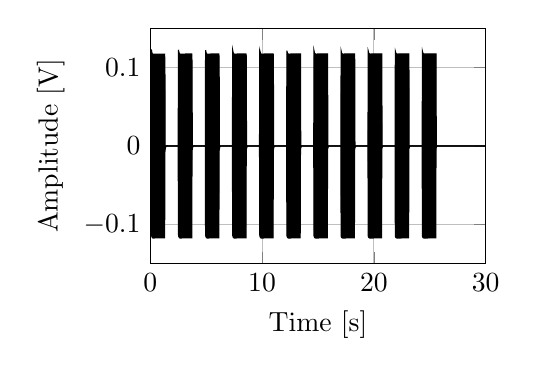
\begin{tikzpicture}

\begin{axis}[%
width=2.3in,
height=1.8in,
at={(0.758in,0.481in)},
xmin=0,
xmax=30,
xmajorgrids,
ymin=-0.15,
ymax=0.15,
ylabel={Amplitude [V]},
xlabel={Time [s]},
ymajorgrids,
axis background/.style={fill=white}
]
\addplot[fill=black,draw=black,forget plot] plot table[row sep=crcr]{%
2.08333333333333e-05	1.58548355102539e-05\\
0.0252733410493827	1.68085098266602e-05\\
0.0505258487654321	1.4185905456543e-05\\
0.0757783564814815	1.75237655639648e-05\\
0.101030864197531	0.122879505157471\\
0.12628337191358	0.120219826698303\\
0.15153587962963	0.118692755699158\\
0.176788387345679	0.117809057235718\\
0.202040895061728	0.117316246032715\\
0.227293402777778	0.117060780525208\\
0.252545910493827	0.116923570632935\\
0.277798418209877	0.116885662078857\\
0.303050925925926	0.116871953010559\\
0.328303433641975	0.11688220500946\\
0.353555941358025	0.116916537284851\\
0.378808449074074	0.116943120956421\\
0.404060956790123	0.116961240768433\\
0.429313464506173	0.116984009742737\\
0.454565972222222	0.116994857788086\\
0.479818479938272	0.11701238155365\\
0.505070987654321	0.117026567459106\\
0.53032349537037	0.117034077644348\\
0.55557600308642	0.117038011550903\\
0.580828510802469	0.117049217224121\\
0.606081018518519	0.117051243782043\\
0.631333526234568	0.117061257362366\\
0.656586033950617	0.117065787315369\\
0.681838541666667	0.117067098617554\\
0.707091049382716	0.117065906524658\\
0.732343557098765	0.117066740989685\\
0.757596064814815	0.1170734167099\\
0.782848572530864	0.117071747779846\\
0.808101080246914	0.117065906524658\\
0.833353587962963	0.117072463035584\\
0.858606095679012	0.117069125175476\\
0.883858603395062	0.117069244384766\\
0.909111111111111	0.117070555686951\\
0.934363618827161	0.11707079410553\\
0.95961612654321	0.117067933082581\\
0.984868634259259	0.117074728012085\\
1.01012114197531	0.117074131965637\\
1.03537364969136	0.117074131965637\\
1.06062615740741	0.117071390151978\\
1.08587866512346	0.117072939872742\\
1.11113117283951	0.11707079410553\\
1.13638368055556	0.117062568664551\\
1.16163618827161	0.117069959640503\\
1.18688869598765	0.117068886756897\\
1.2121412037037	0.117069125175476\\
1.23739371141975	0.11707079410553\\
1.2626462191358	0.117066621780396\\
1.28789872685185	0.117077469825745\\
1.3131512345679	0.10097062587738\\
1.33840374228395	-0.002097487449646\\
1.36365625	-0.000977039337158203\\
1.38890875771605	-0.000357866287231445\\
1.4141612654321	-3.37362289428711e-05\\
1.43941377314815	0.000129342079162598\\
1.4646662808642	0.000192880630493164\\
1.48991878858025	0.000212430953979492\\
1.5151712962963	0.000216245651245117\\
1.54042380401235	0.000203132629394531\\
1.5656763117284	0.000182390213012695\\
1.59092881944444	0.000157356262207031\\
1.61618132716049	0.000135540962219238\\
1.64143383487654	0.000110983848571777\\
1.66668634259259	9.51290130615234e-05\\
1.69193885030864	7.92741775512695e-05\\
1.71719135802469	6.47306442260742e-05\\
1.74244386574074	5.18560409545898e-05\\
1.76769637345679	4.8518180847168e-05\\
1.79294888117284	4.04119491577148e-05\\
1.81820138888889	3.20672988891602e-05\\
1.84345389660494	2.71797180175781e-05\\
1.86870640432099	2.70605087280273e-05\\
1.89395891203704	2.26497650146484e-05\\
1.91921141975309	1.96695327758789e-05\\
1.94446392746914	2.08616256713867e-05\\
1.96971643518519	1.71661376953125e-05\\
1.99496894290123	1.8000602722168e-05\\
2.02022145061728	1.38282775878906e-05\\
2.04547395833333	1.38282775878906e-05\\
2.07072646604938	1.93119049072266e-05\\
2.09597897376543	1.34706497192383e-05\\
2.12123148148148	1.43051147460938e-05\\
2.14648398919753	1.66893005371094e-05\\
2.17173649691358	1.21593475341797e-05\\
2.19698900462963	1.46627426147461e-05\\
2.22224151234568	1.43051147460938e-05\\
2.24749402006173	1.68085098266602e-05\\
2.27274652777778	1.29938125610352e-05\\
2.29799903549383	1.43051147460938e-05\\
2.32325154320988	1.50203704833984e-05\\
2.34850405092593	1.38282775878906e-05\\
2.37375655864198	1.8000602722168e-05\\
2.39900906635802	1.38282775878906e-05\\
2.42426157407407	1.53779983520508e-05\\
2.44951408179012	1.50203704833984e-05\\
2.47476658950617	1.53779983520508e-05\\
2.50001909722222	1.34706497192383e-05\\
2.52527160493827	0.122484803199768\\
2.55052411265432	0.120183825492859\\
2.57577662037037	0.118810296058655\\
2.60102912808642	0.117970824241638\\
2.62628163580247	0.11729907989502\\
2.65153414351852	0.117104768753052\\
2.67678665123457	0.116974830627441\\
2.70203915895062	0.116921067237854\\
2.72729166666667	0.116914510726929\\
2.75254417438272	0.1169353723526\\
2.77779668209877	0.116956114768982\\
2.80304918981481	0.11698317527771\\
2.82830169753086	0.116991639137268\\
2.85355420524691	0.117025017738342\\
2.87880671296296	0.117034912109375\\
2.90405922067901	0.117040872573853\\
2.92931172839506	0.11705756187439\\
2.95456423611111	0.117060780525208\\
2.97981674382716	0.117064714431763\\
3.00506925154321	0.11707592010498\\
3.03032175925926	0.117080450057983\\
3.05557426697531	0.117085814476013\\
3.08082677469136	0.117089986801147\\
3.10607928240741	0.11708927154541\\
3.13133179012346	0.117094159126282\\
3.15658429783951	0.117094993591309\\
3.18183680555556	0.117096304893494\\
3.2070893132716	0.117091774940491\\
3.23234182098765	0.117095589637756\\
3.2575943287037	0.11710250377655\\
3.28284683641975	0.117097496986389\\
3.3080993441358	0.117101430892944\\
3.33335185185185	0.117091298103333\\
3.3586043595679	0.117102146148682\\
3.38385686728395	0.117099285125732\\
3.409109375	0.117094278335571\\
3.43436188271605	0.117102265357971\\
3.4596143904321	0.117097139358521\\
3.48486689814815	0.117097973823547\\
3.5101194058642	0.117094755172729\\
3.53537191358025	0.117103934288025\\
3.5606244212963	0.117095589637756\\
3.58587692901235	0.117089748382568\\
3.61112943672839	0.117098450660706\\
3.63638194444444	0.117092490196228\\
3.66163445216049	0.117099165916443\\
3.68688695987654	0.117096662521362\\
3.71213946759259	0.117095589637756\\
3.73739197530864	0.107169151306152\\
3.76264448302469	-0.00190830230712891\\
3.78789699074074	-0.00088953971862793\\
3.81314949845679	-0.000322818756103516\\
3.83840200617284	-2.62260437011719e-05\\
3.86365451388889	0.000118494033813477\\
3.88890702160494	0.000179886817932129\\
3.91415952932099	0.000197887420654297\\
3.93941203703704	0.000200748443603516\\
3.96466454475309	0.000186920166015625\\
3.98991705246914	0.00016486644744873\\
4.01516956018518	0.000146389007568359\\
4.04042206790123	0.000122785568237305\\
4.06567457561728	0.000103473663330078\\
4.09092708333333	8.85725021362305e-05\\
4.11617959104938	7.18832015991211e-05\\
4.14143209876543	6.04391098022461e-05\\
4.16668460648148	4.92334365844727e-05\\
4.19193711419753	4.10079956054688e-05\\
4.21718962191358	3.55243682861328e-05\\
4.24244212962963	3.12328338623047e-05\\
4.26769463734568	2.58684158325195e-05\\
4.29294714506173	2.26497650146484e-05\\
4.31819965277778	2.08616256713867e-05\\
4.34345216049383	2.09808349609375e-05\\
4.36870466820988	2.00271606445313e-05\\
4.39395717592593	2.00271606445313e-05\\
4.41920968364198	1.51395797729492e-05\\
4.44446219135802	1.71661376953125e-05\\
4.46971469907407	1.8000602722168e-05\\
4.49496720679012	1.21593475341797e-05\\
4.52021971450617	1.78813934326172e-05\\
4.54547222222222	1.58548355102539e-05\\
4.57072472993827	1.59740447998047e-05\\
4.59597723765432	1.51395797729492e-05\\
4.62122974537037	1.26361846923828e-05\\
4.64648225308642	1.33514404296875e-05\\
4.67173476080247	1.29938125610352e-05\\
4.69698726851852	1.54972076416016e-05\\
4.72223977623457	1.2516975402832e-05\\
4.74749228395062	1.37090682983398e-05\\
4.77274479166667	1.62124633789063e-05\\
4.79799729938272	1.43051147460938e-05\\
4.82324980709877	1.45435333251953e-05\\
4.84850231481482	1.37090682983398e-05\\
4.87375482253086	1.59740447998047e-05\\
4.89900733024691	1.33514404296875e-05\\
4.92425983796296	1.54972076416016e-05\\
4.94951234567901	0.122136831283569\\
4.97476485339506	0.120147228240967\\
5.00001736111111	0.118440747261047\\
5.02526986882716	0.117819309234619\\
5.05052237654321	0.11729621887207\\
5.07577488425926	0.117114186286926\\
5.10102739197531	0.116984963417053\\
5.12627989969136	0.116955757141113\\
5.15153240740741	0.116954445838928\\
5.17678491512346	0.116969466209412\\
5.20203742283951	0.116990804672241\\
5.22728993055556	0.11700713634491\\
5.2525424382716	0.117026209831238\\
5.27779494598765	0.117044925689697\\
5.3030474537037	0.117066264152527\\
5.32829996141975	0.117077589035034\\
5.3535524691358	0.11708128452301\\
5.37880497685185	0.117092490196228\\
5.4040574845679	0.117095470428467\\
5.42930999228395	0.117104172706604\\
5.4545625	0.117108106613159\\
5.47981500771605	0.117108941078186\\
5.5050675154321	0.11711061000824\\
5.53032002314815	0.11711597442627\\
5.5555725308642	0.117118954658508\\
5.58082503858025	0.11712646484375\\
5.6060775462963	0.117114663124084\\
5.63133005401235	0.117119193077087\\
5.65658256172839	0.117115139961243\\
5.68183506944444	0.117118835449219\\
5.70708757716049	0.117117285728455\\
5.73234008487654	0.117123961448669\\
5.75759259259259	0.117119669914246\\
5.78284510030864	0.11712384223938\\
5.80809760802469	0.117116451263428\\
5.83335011574074	0.117116451263428\\
5.85860262345679	0.117123365402222\\
5.88385513117284	0.117119312286377\\
5.90910763888889	0.117115020751953\\
5.93436014660494	0.117121458053589\\
5.95961265432099	0.117115020751953\\
5.98486516203704	0.117119312286377\\
6.01011766975309	0.117117285728455\\
6.03537017746914	0.117118358612061\\
6.06062268518518	0.117124676704407\\
6.08587519290123	0.117120981216431\\
6.11112770061728	0.117120504379272\\
6.13638020833333	0.11711847782135\\
6.16163271604938	0.111903429031372\\
6.18688522376543	-0.00175118446350098\\
6.21213773148148	-0.00081324577331543\\
6.23739023919753	-0.000295877456665039\\
6.26264274691358	-1.8000602722168e-05\\
6.28789525462963	0.00011146068572998\\
6.31314776234568	0.00016474723815918\\
6.33840027006173	0.000183939933776855\\
6.36365277777778	0.000184059143066406\\
6.38890528549383	0.000174522399902344\\
6.41415779320988	0.000154018402099609\\
6.43941030092593	0.0001373291015625\\
6.46466280864198	0.000113487243652344\\
6.48991531635802	9.72747802734375e-05\\
6.51516782407407	7.77244567871094e-05\\
6.54042033179012	6.55651092529297e-05\\
6.56567283950617	5.80549240112305e-05\\
6.59092534722222	4.88758087158203e-05\\
6.61617785493827	4.0888786315918e-05\\
6.64143036265432	3.20672988891602e-05\\
6.66668287037037	3.00407409667969e-05\\
6.69193537808642	2.70605087280273e-05\\
6.71718788580247	2.37226486206055e-05\\
6.74244039351852	2.21729278564453e-05\\
6.76769290123457	1.96695327758789e-05\\
6.79294540895062	2.03847885131836e-05\\
6.81819791666667	1.43051147460938e-05\\
6.84345042438272	1.50203704833984e-05\\
6.86870293209877	1.66893005371094e-05\\
6.89395543981481	1.91926956176758e-05\\
6.91920794753086	1.38282775878906e-05\\
6.94446045524691	1.84774398803711e-05\\
6.96971296296296	1.62124633789063e-05\\
6.99496547067901	1.66893005371094e-05\\
7.02021797839506	1.45435333251953e-05\\
7.04547048611111	1.45435333251953e-05\\
7.07072299382716	1.51395797729492e-05\\
7.09597550154321	1.6331672668457e-05\\
7.12122800925926	1.62124633789063e-05\\
7.14648051697531	1.37090682983398e-05\\
7.17173302469136	1.38282775878906e-05\\
7.19698553240741	1.12056732177734e-05\\
7.22223804012346	1.76429748535156e-05\\
7.24749054783951	1.70469284057617e-05\\
7.27274305555556	1.83582305908203e-05\\
7.2979955632716	1.21593475341797e-05\\
7.32324807098765	1.59740447998047e-05\\
7.3485005787037	1.29938125610352e-05\\
7.37375308641975	0.12184476852417\\
7.3990055941358	0.120089888572693\\
7.42425810185185	0.1185302734375\\
7.4495106095679	0.117711305618286\\
7.47476311728395	0.117402195930481\\
7.500015625	0.117144346237183\\
7.52526813271605	0.117019653320313\\
7.5505206404321	0.116984486579895\\
7.57577314814815	0.116981267929077\\
7.6010256558642	0.116997122764587\\
7.62627816358025	0.117016196250916\\
7.6515306712963	0.11703085899353\\
7.67678317901235	0.117055416107178\\
7.70203568672839	0.117057204246521\\
7.72728819444444	0.117087960243225\\
7.75254070216049	0.117092490196228\\
7.77779320987654	0.117108941078186\\
7.80304571759259	0.117111682891846\\
7.82829822530864	0.117115616798401\\
7.85355073302469	0.117121696472168\\
7.87880324074074	0.117124199867249\\
7.90405574845679	0.117127656936646\\
7.92930825617284	0.117123961448669\\
7.95456076388889	0.117131352424622\\
7.97981327160494	0.117124319076538\\
8.00506577932099	0.117135643959045\\
8.03031828703704	0.117133140563965\\
8.05557079475309	0.117125630378723\\
8.08082330246914	0.11713171005249\\
8.10607581018519	0.117137551307678\\
8.13132831790123	0.11713981628418\\
8.15658082561728	0.117139339447021\\
8.18183333333333	0.11713981628418\\
8.20708584104938	0.117138981819153\\
8.23233834876543	0.117137670516968\\
8.25759085648148	0.117145180702209\\
8.28284336419753	0.117140054702759\\
8.30809587191358	0.117145895957947\\
8.33334837962963	0.117139220237732\\
8.35860088734568	0.117133855819702\\
8.38385339506173	0.117145657539368\\
8.40910590277778	0.117128968238831\\
8.43435841049383	0.117143392562866\\
8.45961091820988	0.117140173912048\\
8.48486342592593	0.117136478424072\\
8.51011593364198	0.117136001586914\\
8.53536844135802	0.11714231967926\\
8.56062094907407	0.117137551307678\\
8.58587345679012	0.115118741989136\\
8.61112596450617	-0.00161099433898926\\
8.63637847222222	-0.00074303150177002\\
8.66163097993827	-0.000270724296569824\\
8.68688348765432	-2.08616256713867e-05\\
8.71213599537037	0.00010216236114502\\
8.73738850308642	0.000153899192810059\\
8.76264101080247	0.000169038772583008\\
8.78789351851852	0.000168561935424805\\
8.81314602623457	0.000159859657287598\\
8.83839853395062	0.000145673751831055\\
8.86365104166667	0.000126123428344727\\
8.88890354938272	0.000107169151306152\\
8.91415605709877	9.0479850769043e-05\\
8.93940856481481	7.67707824707031e-05\\
8.96466107253086	6.43730163574219e-05\\
8.98991358024691	5.22136688232422e-05\\
9.01516608796296	4.38690185546875e-05\\
9.04041859567901	3.63588333129883e-05\\
9.06567110339506	3.20672988891602e-05\\
9.09092361111111	2.88486480712891e-05\\
9.11617611882716	2.50339508056641e-05\\
9.14142862654321	2.30073928833008e-05\\
9.16668113425926	2.13384628295898e-05\\
9.19193364197531	1.76429748535156e-05\\
9.21718614969136	2.45571136474609e-05\\
9.24243865740741	1.84774398803711e-05\\
9.26769116512346	1.62124633789063e-05\\
9.29294367283951	1.51395797729492e-05\\
9.31819618055556	1.33514404296875e-05\\
9.34344868827161	1.50203704833984e-05\\
9.36870119598765	1.53779983520508e-05\\
9.3939537037037	1.34706497192383e-05\\
9.41920621141975	1.34706497192383e-05\\
9.4444587191358	1.26361846923828e-05\\
9.46971122685185	1.51395797729492e-05\\
9.4949637345679	1.53779983520508e-05\\
9.52021624228395	1.71661376953125e-05\\
9.54546875	1.38282775878906e-05\\
9.57072125771605	1.51395797729492e-05\\
9.5959737654321	1.62124633789063e-05\\
9.62122627314815	1.54972076416016e-05\\
9.6464787808642	1.59740447998047e-05\\
9.67173128858025	1.58548355102539e-05\\
9.6969837962963	1.54972076416016e-05\\
9.72223630401235	1.76429748535156e-05\\
9.7474888117284	1.29938125610352e-05\\
9.77274131944444	1.84774398803711e-05\\
9.79799382716049	0.121572375297546\\
9.82324633487654	0.120015263557434\\
9.84849884259259	0.118595480918884\\
9.87375135030864	0.117800235748291\\
9.89900385802469	0.117379188537598\\
9.92425636574074	0.117158889770508\\
9.94950887345679	0.11705470085144\\
9.97476138117284	0.117006659507751\\
10.0000138888889	0.117013812065125\\
10.0252663966049	0.117024898529053\\
10.050518904321	0.11704421043396\\
10.075771412037	0.117059230804443\\
10.1010239197531	0.117070555686951\\
10.1262764274691	0.117085576057434\\
10.1515289351852	0.117094159126282\\
10.1767814429012	0.117107629776001\\
10.2020339506173	0.117117285728455\\
10.2272864583333	0.117114663124084\\
10.2525389660494	0.117132663726807\\
10.2777914737654	0.117130637168884\\
10.3030439814815	0.117143034934998\\
10.3282964891975	0.117150545120239\\
10.3535489969136	0.117147207260132\\
10.3788015046296	0.117142677307129\\
10.4040540123457	0.117141008377075\\
10.4293065200617	0.117145657539368\\
10.4545590277778	0.117155909538269\\
10.4798115354938	0.117148160934448\\
10.5050640432099	0.117153406143188\\
10.5303165509259	0.117146730422974\\
10.555569058642	0.117155194282532\\
10.580821566358	0.117154240608215\\
10.6060740740741	0.117156505584717\\
10.6313265817901	0.117158889770508\\
10.6565790895062	0.117149710655212\\
10.6818315972222	0.117150664329529\\
10.7070841049383	0.117155075073242\\
10.7323366126543	0.117151737213135\\
10.7575891203704	0.117151379585266\\
10.7828416280864	0.117152571678162\\
10.8080941358025	0.117152333259583\\
10.8333466435185	0.11715304851532\\
10.8585991512346	0.117153167724609\\
10.8838516589506	0.11715304851532\\
10.9091041666667	0.117150545120239\\
10.9343566743827	0.117151021957397\\
10.9596091820988	0.117149233818054\\
10.9848616898148	0.117151856422424\\
11.0101141975309	0.116843819618225\\
11.0353667052469	-0.00150108337402344\\
11.060619212963	-0.000692605972290039\\
11.085871720679	-0.000258207321166992\\
11.1111242283951	-1.95503234863281e-05\\
11.1363767361111	9.22679901123047e-05\\
11.1616292438272	0.000141143798828125\\
11.1868817515432	0.000156521797180176\\
11.2121342592593	0.000157713890075684\\
11.2373867669753	0.000151872634887695\\
11.2626392746914	0.000136852264404297\\
11.2878917824074	0.000113487243652344\\
11.3131442901235	9.94205474853516e-05\\
11.3383967978395	9.10758972167969e-05\\
11.3636493055556	7.02142715454102e-05\\
11.3889018132716	5.93662261962891e-05\\
11.4141543209877	5.68628311157227e-05\\
11.4394068287037	4.20808792114258e-05\\
11.4646593364198	3.83853912353516e-05\\
11.4899118441358	3.30209732055664e-05\\
11.5151643518519	2.58684158325195e-05\\
11.5404168595679	2.37226486206055e-05\\
11.565669367284	2.41994857788086e-05\\
11.590921875	2.21729278564453e-05\\
11.6161743827161	1.96695327758789e-05\\
11.6414268904321	1.70469284057617e-05\\
11.6666793981481	1.93119049072266e-05\\
11.6919319058642	1.8000602722168e-05\\
11.7171844135802	2.00271606445313e-05\\
11.7424369212963	1.6331672668457e-05\\
11.7676894290123	1.62124633789063e-05\\
11.7929419367284	1.68085098266602e-05\\
11.8181944444444	1.6331672668457e-05\\
11.8434469521605	1.46627426147461e-05\\
11.8686994598765	1.75237655639648e-05\\
11.8939519675926	1.29938125610352e-05\\
11.9192044753086	1.33514404296875e-05\\
11.9444569830247	1.59740447998047e-05\\
11.9697094907407	1.6331672668457e-05\\
11.9949619984568	1.38282775878906e-05\\
12.0202145061728	1.28746032714844e-05\\
12.0454670138889	1.6331672668457e-05\\
12.0707195216049	1.71661376953125e-05\\
12.095972029321	1.38282775878906e-05\\
12.121224537037	1.37090682983398e-05\\
12.1464770447531	1.58548355102539e-05\\
12.1717295524691	2.00271606445313e-05\\
12.1969820601852	1.51395797729492e-05\\
12.2222345679012	0.121322989463806\\
12.2474870756173	0.119430780410767\\
12.2727395833333	0.118337512016296\\
12.2979920910494	0.117706418037415\\
12.3232445987654	0.117356300354004\\
12.3484971064815	0.117170214653015\\
12.3737496141975	0.117075443267822\\
12.3990021219136	0.117034077644348\\
12.4242546296296	0.117026567459106\\
12.4495071373457	0.117044925689697\\
12.4747596450617	0.117059230804443\\
12.5000121527778	0.117071628570557\\
12.5252646604938	0.117092967033386\\
12.5505171682099	0.11710512638092\\
12.5757696759259	0.11711061000824\\
12.601022183642	0.11711311340332\\
12.626274691358	0.117130517959595\\
12.6515271990741	0.11713719367981\\
12.6767797067901	0.117137312889099\\
12.7020322145062	0.117154717445374\\
12.7272847222222	0.11714768409729\\
12.7525372299383	0.117150068283081\\
12.7777897376543	0.117154836654663\\
12.8030422453704	0.117156863212585\\
12.8282947530864	0.117158055305481\\
12.8535472608025	0.117160201072693\\
12.8787997685185	0.117162346839905\\
12.9040522762346	0.11716103553772\\
12.9293047839506	0.11715841293335\\
12.9545572916667	0.117161393165588\\
12.9798097993827	0.117159247398376\\
13.0050623070988	0.117155909538269\\
13.0303148148148	0.117157340049744\\
13.0555673225309	0.117167353630066\\
13.0808198302469	0.117165088653564\\
13.106072337963	0.117163062095642\\
13.131324845679	0.117162704467773\\
13.1565773533951	0.117162704467773\\
13.1818298611111	0.117157697677612\\
13.2070823688272	0.117157697677612\\
13.2323348765432	0.11716103553772\\
13.2575873842593	0.117165923118591\\
13.2828398919753	0.117160677909851\\
13.3080923996914	0.117161750793457\\
13.3333449074074	0.117158889770508\\
13.3585974151235	0.117161512374878\\
13.3838499228395	0.1171635389328\\
13.4091024305556	0.117165565490723\\
13.4343549382716	0.117153167724609\\
13.4596074459877	-0.0013965368270874\\
13.4848599537037	-0.000646233558654785\\
13.5101124614198	-0.000239133834838867\\
13.5353649691358	-1.95503234863281e-05\\
13.5606174768519	9.13143157958984e-05\\
13.5858699845679	0.000134706497192383\\
13.611122492284	0.000146031379699707\\
13.636375	0.000151395797729492\\
13.6616275077161	0.000142693519592285\\
13.6868800154321	0.000128626823425293\\
13.7121325231481	0.000111937522888184\\
13.7373850308642	9.6440315246582e-05\\
13.7626375385802	8.13007354736328e-05\\
13.7878900462963	6.68764114379883e-05\\
13.8131425540123	5.68628311157227e-05\\
13.8383950617284	4.76837158203125e-05\\
13.8636475694444	3.93390655517578e-05\\
13.8889000771605	3.4332275390625e-05\\
13.9141525848765	3.29017639160156e-05\\
13.9394050925926	2.76565551757813e-05\\
13.9646576003086	2.63452529907227e-05\\
13.9899101080247	2.03847885131836e-05\\
14.0151626157407	2.09808349609375e-05\\
14.0404151234568	2.0146369934082e-05\\
14.0656676311728	1.84774398803711e-05\\
14.0909201388889	1.54972076416016e-05\\
14.1161726466049	1.54972076416016e-05\\
14.141425154321	1.28746032714844e-05\\
14.166677662037	1.68085098266602e-05\\
14.1919301697531	1.50203704833984e-05\\
14.2171826774691	1.43051147460938e-05\\
14.2424351851852	1.34706497192383e-05\\
14.2676876929012	1.21593475341797e-05\\
14.2929402006173	1.54972076416016e-05\\
14.3181927083333	1.51395797729492e-05\\
14.3434452160494	1.95503234863281e-05\\
14.3686977237654	1.83582305908203e-05\\
14.3939502314815	1.37090682983398e-05\\
14.4192027391975	1.84774398803711e-05\\
14.4444552469136	1.87158584594727e-05\\
14.4697077546296	1.54972076416016e-05\\
14.4949602623457	1.4185905456543e-05\\
14.5202127700617	1.51395797729492e-05\\
14.5454652777778	1.66893005371094e-05\\
14.5707177854938	1.4185905456543e-05\\
14.5959702932099	1.54972076416016e-05\\
14.6212228009259	1.37090682983398e-05\\
14.646475308642	0.121119737625122\\
14.671727816358	0.119396567344666\\
14.6969803240741	0.11837899684906\\
14.7222328317901	0.117777705192566\\
14.7474853395062	0.117345333099365\\
14.7727378472222	0.117175102233887\\
14.7979903549383	0.117093920707703\\
14.8232428626543	0.117048859596252\\
14.8484953703704	0.117047071456909\\
14.8737478780864	0.117058277130127\\
14.8990003858025	0.117074608802795\\
14.9242528935185	0.117087244987488\\
14.9495054012346	0.117104649543762\\
14.9747579089506	0.117116332054138\\
15.0000104166667	0.11712384223938\\
15.0252629243827	0.117133021354675\\
15.0505154320988	0.11713981628418\\
15.0757679398148	0.117148160934448\\
15.1010204475309	0.117156505584717\\
15.1262729552469	0.117164254188538\\
15.151525462963	0.11716091632843\\
15.176777970679	0.117161750793457\\
15.2020304783951	0.117171049118042\\
15.2272829861111	0.117166519165039\\
15.2525354938272	0.117164015769959\\
15.2777880015432	0.117171049118042\\
15.3030405092593	0.117171764373779\\
15.3282930169753	0.117170691490173\\
15.3535455246914	0.117169380187988\\
15.3787980324074	0.117179274559021\\
15.4040505401235	0.117166757583618\\
15.4293030478395	0.117171049118042\\
15.4545555555556	0.117173075675964\\
15.4798080632716	0.117171049118042\\
15.5050605709877	0.117173194885254\\
15.5303130787037	0.117174744606018\\
15.5555655864198	0.117173433303833\\
15.5808180941358	0.117167592048645\\
15.6060706018519	0.117179393768311\\
15.6313231095679	0.117175579071045\\
15.656575617284	0.117165207862854\\
15.681828125	0.117167353630066\\
15.7070806327161	0.117172241210938\\
15.7323331404321	0.117172360420227\\
15.7575856481481	0.117165684700012\\
15.7828381558642	0.117171883583069\\
15.8080906635802	0.117170095443726\\
15.8333431712963	0.117170929908752\\
15.8585956790123	0.117159366607666\\
15.8838481867284	-0.00130629539489746\\
15.9091006944444	-0.000602126121520996\\
15.9343532021605	-0.00022435188293457\\
15.9596057098765	-1.58548355102539e-05\\
15.9848582175926	8.30888748168945e-05\\
16.0101107253086	0.000125527381896973\\
16.0353632330247	0.000137686729431152\\
16.0606157407407	0.000142335891723633\\
16.0858682484568	0.000131964683532715\\
16.1111207561728	0.000119805335998535\\
16.1363732638889	0.000101089477539063\\
16.1616257716049	9.02414321899414e-05\\
16.186878279321	7.43865966796875e-05\\
16.212130787037	6.46114349365234e-05\\
16.2373832947531	5.60283660888672e-05\\
16.2626358024691	4.8518180847168e-05\\
16.2878883101852	4.18424606323242e-05\\
16.3131408179012	3.38554382324219e-05\\
16.3383933256173	3.08752059936523e-05\\
16.3636458333333	2.53915786743164e-05\\
16.3888983410494	2.45571136474609e-05\\
16.4141508487654	2.46763229370117e-05\\
16.4394033564815	1.96695327758789e-05\\
16.4646558641975	1.8000602722168e-05\\
16.4899083719136	1.70469284057617e-05\\
16.5151608796296	1.62124633789063e-05\\
16.5404133873457	2.16960906982422e-05\\
16.5656658950617	1.50203704833984e-05\\
16.5909184027778	2.16960906982422e-05\\
16.6161709104938	1.33514404296875e-05\\
16.6414234182099	1.68085098266602e-05\\
16.6666759259259	1.51395797729492e-05\\
16.691928433642	1.51395797729492e-05\\
16.717180941358	1.59740447998047e-05\\
16.7424334490741	1.43051147460938e-05\\
16.7676859567901	1.46627426147461e-05\\
16.7929384645062	1.46627426147461e-05\\
16.8181909722222	1.59740447998047e-05\\
16.8434434799383	1.6331672668457e-05\\
16.8686959876543	1.84774398803711e-05\\
16.8939484953704	1.59740447998047e-05\\
16.9192010030864	1.95503234863281e-05\\
16.9444535108025	1.71661376953125e-05\\
16.9697060185185	1.50203704833984e-05\\
16.9949585262346	1.50203704833984e-05\\
17.0202110339506	1.43051147460938e-05\\
17.0454635416667	1.59740447998047e-05\\
17.0707160493827	0.120926856994629\\
17.0959685570988	0.119378209114075\\
17.1212210648148	0.118203639984131\\
17.1464735725309	0.117694973945618\\
17.1717260802469	0.117335319519043\\
17.196978587963	0.117192268371582\\
17.222231095679	0.117097616195679\\
17.2474836033951	0.117066740989685\\
17.2727361111111	0.11705756187439\\
17.2979886188272	0.1170654296875\\
17.3232411265432	0.117082476615906\\
17.3484936342593	0.117109179496765\\
17.3737461419753	0.117106676101685\\
17.3989986496914	0.117122173309326\\
17.4242511574074	0.117138981819153\\
17.4495036651235	0.117141842842102\\
17.4747561728395	0.117156863212585\\
17.5000086805556	0.117157340049744\\
17.5252611882716	0.117165088653564\\
17.5505136959877	0.117173194885254\\
17.5757662037037	0.117165088653564\\
17.6010187114198	0.117175698280334\\
17.6262712191358	0.117171883583069\\
17.6515237268519	0.117169857025146\\
17.6767762345679	0.117180228233337\\
17.702028742284	0.117179036140442\\
17.72728125	0.117185115814209\\
17.7525337577161	0.117179036140442\\
17.7777862654321	0.117178201675415\\
17.8030387731481	0.117188215255737\\
17.8282912808642	0.11717689037323\\
17.8535437885803	0.117181420326233\\
17.8787962962963	0.117181420326233\\
17.9040488040123	0.117183208465576\\
17.9293013117284	0.11718487739563\\
17.9545538194444	0.117179036140442\\
17.9798063271605	0.117180943489075\\
18.0050588348765	0.117177724838257\\
18.0303113425926	0.117183923721313\\
18.0555638503086	0.117178440093994\\
18.0808163580247	0.117181062698364\\
18.1060688657407	0.117178916931152\\
18.1313213734568	0.117185592651367\\
18.1565738811728	0.117179751396179\\
18.1818263888889	0.117183208465576\\
18.2070788966049	0.117183208465576\\
18.232331404321	0.117177605628967\\
18.257583912037	0.117175698280334\\
18.2828364197531	0.117178916931152\\
18.3080889274691	-0.00123071670532227\\
18.3333414351852	-0.000575661659240723\\
18.3585939429012	-0.000205278396606445\\
18.3838464506173	-1.95503234863281e-05\\
18.4090989583333	7.77244567871094e-05\\
18.4343514660494	0.000117778778076172\\
18.4596039737654	0.000131130218505859\\
18.4848564814815	0.000134706497192383\\
18.5101089891975	0.000125527381896973\\
18.5353614969136	0.000114679336547852\\
18.5606140046296	0.000100970268249512\\
18.5858665123457	8.67843627929688e-05\\
18.6111190200617	7.93933868408203e-05\\
18.6363715277778	6.27040863037109e-05\\
18.6616240354938	5.00679016113281e-05\\
18.6868765432099	4.55379486083984e-05\\
18.7121290509259	3.88622283935547e-05\\
18.737381558642	3.17096710205078e-05\\
18.762634066358	2.83718109130859e-05\\
18.7878865740741	2.50339508056641e-05\\
18.8131390817901	2.55107879638672e-05\\
18.8383915895062	2.08616256713867e-05\\
18.8636440972222	1.96695327758789e-05\\
18.8888966049383	2.26497650146484e-05\\
18.9141491126543	1.6331672668457e-05\\
18.9394016203704	1.6331672668457e-05\\
18.9646541280864	1.91926956176758e-05\\
18.9899066358025	1.38282775878906e-05\\
19.0151591435185	1.4185905456543e-05\\
19.0404116512346	1.6331672668457e-05\\
19.0656641589506	1.59740447998047e-05\\
19.0909166666667	1.54972076416016e-05\\
19.1161691743827	1.43051147460938e-05\\
19.1414216820988	1.58548355102539e-05\\
19.1666741898148	1.38282775878906e-05\\
19.1919266975309	1.4185905456543e-05\\
19.2171792052469	1.45435333251953e-05\\
19.242431712963	1.29938125610352e-05\\
19.267684220679	1.51395797729492e-05\\
19.2929367283951	1.2516975402832e-05\\
19.3181892361111	1.6331672668457e-05\\
19.3434417438272	1.43051147460938e-05\\
19.3686942515432	1.54972076416016e-05\\
19.3939467592593	1.45435333251953e-05\\
19.4191992669753	1.91926956176758e-05\\
19.4444517746914	1.46627426147461e-05\\
19.4697042824074	1.50203704833984e-05\\
19.4949567901235	0.120749235153198\\
19.5202092978395	0.119339823722839\\
19.5454618055556	0.11822497844696\\
19.5707143132716	0.117634654045105\\
19.5959668209877	0.117380023002625\\
19.6212193287037	0.117199420928955\\
19.6464718364198	0.117104649543762\\
19.6717243441358	0.117072939872742\\
19.6969768518519	0.117077469825745\\
19.7222293595679	0.117088317871094\\
19.747481867284	0.117100834846497\\
19.772734375	0.11710250377655\\
19.797986882716	0.117123484611511\\
19.8232393904321	0.117137312889099\\
19.8484918981482	0.117151379585266\\
19.8737444058642	0.117156386375427\\
19.8989969135802	0.117152690887451\\
19.9242494212963	0.117169737815857\\
19.9495019290123	0.117164373397827\\
19.9747544367284	0.117177248001099\\
20.0000069444444	0.117178916931152\\
20.0252594521605	0.117188096046448\\
20.0505119598765	0.11718487739563\\
20.0757644675926	0.117183446884155\\
20.1010169753086	0.117179036140442\\
20.1262694830247	0.117183208465576\\
20.1515219907407	0.117185711860657\\
20.1767744984568	0.117181539535522\\
20.2020270061728	0.117182374000549\\
20.2272795138889	0.117188215255737\\
20.2525320216049	0.117190599441528\\
20.277784529321	0.117191076278687\\
20.303037037037	0.117186903953552\\
20.3282895447531	0.117191076278687\\
20.3535420524691	0.11718475818634\\
20.3787945601852	0.117183089256287\\
20.4040470679012	0.117189407348633\\
20.4292995756173	0.117185592651367\\
20.4545520833333	0.117185592651367\\
20.4798045910494	0.117187738418579\\
20.5050570987654	0.117182731628418\\
20.5303096064815	0.117193102836609\\
20.5555621141975	0.117186784744263\\
20.5808146219136	0.117185711860657\\
20.6060671296296	0.117184281349182\\
20.6313196373457	0.11718487739563\\
20.6565721450617	0.117187261581421\\
20.6818246527778	0.117189764976501\\
20.7070771604938	0.117178916931152\\
20.7323296682099	-0.00116312503814697\\
20.7575821759259	-0.000541448593139648\\
20.782834683642	-0.00019681453704834\\
20.808087191358	-1.38282775878906e-05\\
20.8333396990741	7.64131546020508e-05\\
20.8585922067901	0.000113129615783691\\
20.8838447145062	0.000133037567138672\\
20.9090972222222	0.000124454498291016\\
20.9343497299383	0.000122189521789551\\
20.9596022376543	0.000113964080810547\\
20.9848547453704	9.21487808227539e-05\\
21.0101072530864	8.13007354736328e-05\\
21.0353597608025	6.79492950439453e-05\\
21.0606122685185	5.97238540649414e-05\\
21.0858647762346	5.17368316650391e-05\\
21.1111172839506	4.20808792114258e-05\\
21.1363697916667	3.83853912353516e-05\\
21.1616222993827	3.33786010742188e-05\\
21.1868748070988	2.76565551757813e-05\\
21.2121273148148	2.55107879638672e-05\\
21.2373798225309	2.20537185668945e-05\\
21.2626323302469	2.0146369934082e-05\\
21.287884837963	1.75237655639648e-05\\
21.313137345679	1.70469284057617e-05\\
21.3383898533951	1.87158584594727e-05\\
21.3636423611111	1.59740447998047e-05\\
21.3888948688272	1.50203704833984e-05\\
21.4141473765432	2.26497650146484e-05\\
21.4393998842593	1.58548355102539e-05\\
21.4646523919753	1.59740447998047e-05\\
21.4899048996914	1.8000602722168e-05\\
21.5151574074074	1.37090682983398e-05\\
21.5404099151235	1.33514404296875e-05\\
21.5656624228395	1.71661376953125e-05\\
21.5909149305556	1.59740447998047e-05\\
21.6161674382716	1.43051147460938e-05\\
21.6414199459877	1.58548355102539e-05\\
21.6666724537037	1.54972076416016e-05\\
21.6919249614198	1.46627426147461e-05\\
21.7171774691358	1.6331672668457e-05\\
21.7424299768519	1.54972076416016e-05\\
21.7676824845679	1.59740447998047e-05\\
21.792934992284	1.53779983520508e-05\\
21.8181875	1.46627426147461e-05\\
21.8434400077161	1.58548355102539e-05\\
21.8686925154321	1.88350677490234e-05\\
21.8939450231481	1.58548355102539e-05\\
21.9191975308642	0.120596170425415\\
21.9444500385803	0.119302153587341\\
21.9697025462963	0.118262887001038\\
21.9949550540123	0.117682576179504\\
22.0202075617284	0.117359280586243\\
22.0454600694444	0.117203950881958\\
22.0707125771605	0.117124319076538\\
22.0959650848765	0.117083430290222\\
22.1212175925926	0.117083787918091\\
22.1464701003086	0.117091298103333\\
22.1717226080247	0.11711061000824\\
22.1969751157407	0.117120146751404\\
22.2222276234568	0.117133498191834\\
22.2474801311728	0.11713969707489\\
22.2727326388889	0.117153167724609\\
22.2979851466049	0.117171049118042\\
22.323237654321	0.117168068885803\\
22.348490162037	0.117171049118042\\
22.3737426697531	0.117175102233887\\
22.3989951774691	0.117181539535522\\
22.4242476851852	0.117188453674316\\
22.4495001929012	0.117183089256287\\
22.4747527006173	0.117186546325684\\
22.5000052083333	0.11718225479126\\
22.5252577160494	0.117189288139343\\
22.5505102237654	0.117201447486877\\
22.5757627314815	0.117195129394531\\
22.6010152391975	0.117189049720764\\
22.6262677469136	0.117189407348633\\
22.6515202546296	0.117195129394531\\
22.6767727623457	0.117196083068848\\
22.7020252700617	0.117192625999451\\
22.7272777777778	0.117191791534424\\
22.7525302854938	0.117183923721313\\
22.7777827932099	0.117191076278687\\
22.8030353009259	0.117192625999451\\
22.828287808642	0.117190718650818\\
22.853540316358	0.117193937301636\\
22.8787928240741	0.117192268371582\\
22.9040453317901	0.117197394371033\\
22.9292978395062	0.117189764976501\\
22.9545503472222	0.117191076278687\\
22.9798028549383	0.117191910743713\\
23.0050553626543	0.117190718650818\\
23.0303078703704	0.117206454277039\\
23.0555603780864	0.117193937301636\\
23.0808128858025	0.117188215255737\\
23.1060653935185	0.117187261581421\\
23.1313179012346	0.117185950279236\\
23.1565704089506	-0.00110018253326416\\
23.1818229166667	-0.000504493713378906\\
23.2070754243827	-0.000182390213012695\\
23.2323279320988	-1.07288360595703e-05\\
23.2575804398148	7.00950622558594e-05\\
23.2828329475309	0.000109672546386719\\
23.3080854552469	0.000119686126708984\\
23.333337962963	0.000123143196105957\\
23.358590470679	0.000113606452941895\\
23.3838429783951	0.000101923942565918\\
23.4090954861111	9.19103622436523e-05\\
23.4343479938272	7.77244567871094e-05\\
23.4596005015432	6.52074813842773e-05\\
23.4848530092593	6.05583190917969e-05\\
23.5101055169753	5.04255294799805e-05\\
23.5353580246914	4.22000885009766e-05\\
23.5606105324074	3.45706939697266e-05\\
23.5858630401235	3.13520431518555e-05\\
23.6111155478395	2.62260437011719e-05\\
23.6363680555556	2.288818359375e-05\\
23.6616205632716	2.21729278564453e-05\\
23.6868730709877	2.53915786743164e-05\\
23.7121255787037	1.87158584594727e-05\\
23.7373780864198	1.8000602722168e-05\\
23.7626305941358	2.20537185668945e-05\\
23.7878831018519	1.71661376953125e-05\\
23.8131356095679	1.87158584594727e-05\\
23.838388117284	1.68085098266602e-05\\
23.863640625	1.50203704833984e-05\\
23.888893132716	1.37090682983398e-05\\
23.9141456404321	1.59740447998047e-05\\
23.9393981481482	1.38282775878906e-05\\
23.9646506558642	1.8000602722168e-05\\
23.9899031635802	1.4185905456543e-05\\
24.0151556712963	1.6331672668457e-05\\
24.0404081790123	1.43051147460938e-05\\
24.0656606867284	1.76429748535156e-05\\
24.0909131944444	1.43051147460938e-05\\
24.1161657021605	1.33514404296875e-05\\
24.1414182098765	1.75237655639648e-05\\
24.1666707175926	1.62124633789063e-05\\
24.1919232253086	1.51395797729492e-05\\
24.2171757330247	2.00271606445313e-05\\
24.2424282407407	1.66893005371094e-05\\
24.2676807484568	1.75237655639648e-05\\
24.2929332561728	1.38282775878906e-05\\
24.3181857638889	1.62124633789063e-05\\
24.3434382716049	0.12043833732605\\
24.368690779321	0.118965148925781\\
24.393943287037	0.118106365203857\\
24.4191957947531	0.117617845535278\\
24.4444483024691	0.117347836494446\\
24.4697008101852	0.11720860004425\\
24.4949533179012	0.117131352424622\\
24.5202058256173	0.117092490196228\\
24.5454583333333	0.117092490196228\\
24.5707108410494	0.117101430892944\\
24.5959633487654	0.117108345031738\\
24.6212158564815	0.117124795913696\\
24.6464683641975	0.117135047912598\\
24.6717208719136	0.117146372795105\\
24.6969733796296	0.1171555519104\\
24.7222258873457	0.117163419723511\\
24.7474783950617	0.117166876792908\\
24.7727309027778	0.11717677116394\\
24.7979834104938	0.117181062698364\\
24.8232359182099	0.117178559303284\\
24.8484884259259	0.117177367210388\\
24.873740933642	0.117191076278687\\
24.898993441358	0.117182374000549\\
24.9242459490741	0.117188096046448\\
24.9494984567901	0.117188215255737\\
24.9747509645062	0.117191433906555\\
25.0000034722222	0.117191791534424\\
25.0252559799383	0.117189884185791\\
25.0505084876543	0.117188930511475\\
25.0757609953704	0.117192387580872\\
25.1010135030864	0.117194890975952\\
25.1262660108025	0.117196440696716\\
25.1515185185185	0.117193102836609\\
25.1767710262346	0.117185950279236\\
25.2020235339506	0.117194771766663\\
25.2272760416667	0.117188453674316\\
25.2525285493827	0.11719810962677\\
25.2777810570988	0.117190718650818\\
25.3030335648148	0.117195248603821\\
25.3282860725309	0.117193222045898\\
25.3535385802469	0.117190957069397\\
25.378791087963	0.117193579673767\\
25.404043595679	0.117189049720764\\
25.4292961033951	0.117193937301636\\
25.4545486111111	0.11718761920929\\
25.4798011188272	0.117189288139343\\
25.5050536265432	0.117192268371582\\
25.5303061342593	0.117191433906555\\
25.5555586419753	0.117186069488525\\
25.5808111496914	-0.00104260444641113\\
25.6060636574074	-0.000486850738525391\\
25.6313161651235	-0.000173211097717285\\
25.6565686728395	-1.40666961669922e-05\\
25.6818211805556	6.63995742797852e-05\\
25.7070736882716	0.000101447105407715\\
25.7323261959877	0.000113844871520996\\
25.7575787037037	0.000117182731628418\\
25.7828312114198	0.000109672546386719\\
25.8080837191358	9.71555709838867e-05\\
25.8333362268519	8.71419906616211e-05\\
25.8585887345679	7.22408294677734e-05\\
25.883841242284	6.3776969909668e-05\\
25.90909375	5.51939010620117e-05\\
25.9343462577161	4.63724136352539e-05\\
25.9595987654321	4.00543212890625e-05\\
25.9848512731481	3.50475311279297e-05\\
26.0101037808642	3.21865081787109e-05\\
26.0353562885803	2.70605087280273e-05\\
26.0606087962963	2.33650207519531e-05\\
26.0858613040123	2.33650207519531e-05\\
26.1111138117284	2.20537185668945e-05\\
26.1363663194444	1.96695327758789e-05\\
26.1616188271605	1.75237655639648e-05\\
26.1868713348765	1.8000602722168e-05\\
26.2121238425926	1.59740447998047e-05\\
26.2373763503086	1.46627426147461e-05\\
26.2626288580247	1.59740447998047e-05\\
26.2878813657407	1.83582305908203e-05\\
26.3131338734568	1.6331672668457e-05\\
26.3383863811728	1.58548355102539e-05\\
26.3636388888889	1.51395797729492e-05\\
26.3888913966049	1.75237655639648e-05\\
26.414143904321	1.43051147460938e-05\\
26.439396412037	1.8000602722168e-05\\
26.4646489197531	1.59740447998047e-05\\
26.4899014274691	1.38282775878906e-05\\
26.5151539351852	1.45435333251953e-05\\
26.5404064429012	1.62124633789063e-05\\
26.5656589506173	1.33514404296875e-05\\
26.5909114583333	1.59740447998047e-05\\
26.6161639660494	1.84774398803711e-05\\
26.6414164737654	1.6331672668457e-05\\
26.6666689814815	1.71661376953125e-05\\
26.6919214891975	1.53779983520508e-05\\
26.7171739969136	1.75237655639648e-05\\
26.7424265046296	1.54972076416016e-05\\
26.7676790123457	1.58548355102539e-05\\
26.7929315200617	1.43051147460938e-05\\
26.8181840277778	1.87158584594727e-05\\
26.8434365354938	1.6331672668457e-05\\
26.8686890432099	1.88350677490234e-05\\
26.8939415509259	1.75237655639648e-05\\
26.919194058642	1.8000602722168e-05\\
26.944446566358	1.68085098266602e-05\\
26.9696990740741	1.71661376953125e-05\\
26.9949515817901	1.6331672668457e-05\\
27.0202040895062	1.6331672668457e-05\\
27.0454565972222	1.66893005371094e-05\\
27.0707091049383	1.51395797729492e-05\\
27.0959616126543	1.88350677490234e-05\\
27.1212141203704	1.37090682983398e-05\\
27.1464666280864	1.54972076416016e-05\\
27.1717191358025	1.28746032714844e-05\\
27.1969716435185	1.58548355102539e-05\\
27.2222241512346	1.54972076416016e-05\\
27.2474766589506	1.66893005371094e-05\\
27.2727291666667	1.71661376953125e-05\\
27.2979816743827	1.58548355102539e-05\\
27.3232341820988	1.45435333251953e-05\\
27.3484866898148	1.59740447998047e-05\\
27.3737391975309	1.6331672668457e-05\\
27.3989917052469	1.46627426147461e-05\\
27.424244212963	1.87158584594727e-05\\
27.449496720679	1.75237655639648e-05\\
27.4747492283951	1.95503234863281e-05\\
27.5000017361111	1.58548355102539e-05\\
27.5252542438272	1.58548355102539e-05\\
27.5505067515432	1.70469284057617e-05\\
27.5757592592593	1.58548355102539e-05\\
27.6010117669753	1.53779983520508e-05\\
27.6262642746914	1.66893005371094e-05\\
27.6515167824074	1.88350677490234e-05\\
27.6767692901235	1.91926956176758e-05\\
27.7020217978395	1.59740447998047e-05\\
27.7272743055556	1.66893005371094e-05\\
27.7525268132716	1.78813934326172e-05\\
27.7777793209877	1.66893005371094e-05\\
27.8030318287037	1.37090682983398e-05\\
27.8282843364198	1.6331672668457e-05\\
27.8535368441358	1.4185905456543e-05\\
27.8787893518519	1.75237655639648e-05\\
27.9040418595679	1.88350677490234e-05\\
27.929294367284	1.68085098266602e-05\\
27.954546875	1.53779983520508e-05\\
27.979799382716	1.93119049072266e-05\\
28.0050518904321	1.8000602722168e-05\\
28.0303043981482	1.53779983520508e-05\\
28.0555569058642	2.16960906982422e-05\\
28.0808094135802	2.13384628295898e-05\\
28.1060619212963	1.68085098266602e-05\\
28.1313144290123	1.43051147460938e-05\\
28.1565669367284	1.54972076416016e-05\\
28.1818194444444	1.58548355102539e-05\\
28.2070719521605	1.68085098266602e-05\\
28.2323244598765	1.76429748535156e-05\\
28.2575769675926	1.59740447998047e-05\\
28.2828294753086	1.87158584594727e-05\\
28.3080819830247	1.6331672668457e-05\\
28.3333344907407	1.75237655639648e-05\\
28.3585869984568	1.51395797729492e-05\\
28.3838395061728	1.4185905456543e-05\\
28.4090920138889	1.51395797729492e-05\\
28.4343445216049	1.76429748535156e-05\\
28.459597029321	1.51395797729492e-05\\
28.484849537037	1.71661376953125e-05\\
28.5101020447531	1.88350677490234e-05\\
28.5353545524691	1.68085098266602e-05\\
28.5606070601852	1.6331672668457e-05\\
28.5858595679012	1.78813934326172e-05\\
28.6111120756173	1.6331672668457e-05\\
28.6363645833333	1.71661376953125e-05\\
28.6616170910494	1.88350677490234e-05\\
28.6868695987654	1.71661376953125e-05\\
28.7121221064815	1.71661376953125e-05\\
28.7373746141975	1.8000602722168e-05\\
28.7626271219136	1.62124633789063e-05\\
28.7878796296296	1.75237655639648e-05\\
28.8131321373457	1.76429748535156e-05\\
28.8383846450617	1.75237655639648e-05\\
28.8636371527778	1.6331672668457e-05\\
28.8888896604938	1.70469284057617e-05\\
28.9141421682099	1.70469284057617e-05\\
28.9393946759259	2.03847885131836e-05\\
28.964647183642	1.87158584594727e-05\\
28.989899691358	1.76429748535156e-05\\
29.0151521990741	1.53779983520508e-05\\
29.0404047067901	1.68085098266602e-05\\
29.0656572145062	2.00271606445313e-05\\
29.0909097222222	1.68085098266602e-05\\
29.1161622299383	1.70469284057617e-05\\
29.1414147376543	1.50203704833984e-05\\
29.1666672453704	1.84774398803711e-05\\
29.1919197530864	1.66893005371094e-05\\
29.2171722608025	1.76429748535156e-05\\
29.2424247685185	1.53779983520508e-05\\
29.2676772762346	1.43051147460938e-05\\
29.2929297839506	1.6331672668457e-05\\
29.3181822916667	1.71661376953125e-05\\
29.3434347993827	1.95503234863281e-05\\
29.3686873070988	1.58548355102539e-05\\
29.3939398148148	2.00271606445313e-05\\
29.4191923225309	1.43051147460938e-05\\
29.4444448302469	1.54972076416016e-05\\
29.469697337963	1.59740447998047e-05\\
29.494949845679	1.76429748535156e-05\\
29.5202023533951	1.53779983520508e-05\\
29.5454548611111	1.66893005371094e-05\\
29.5707073688272	1.45435333251953e-05\\
29.5959598765432	1.76429748535156e-05\\
29.6212123842593	1.59740447998047e-05\\
29.6464648919753	1.4185905456543e-05\\
29.6717173996914	1.75237655639648e-05\\
29.6969699074074	1.83582305908203e-05\\
29.7222224151235	2.13384628295898e-05\\
29.7474749228395	1.84774398803711e-05\\
29.7727274305556	1.62124633789063e-05\\
29.7979799382716	1.83582305908203e-05\\
29.8232324459877	2.00271606445313e-05\\
29.8484849537037	1.93119049072266e-05\\
29.8737374614198	1.53779983520508e-05\\
29.8989899691358	1.6331672668457e-05\\
29.9242424768519	1.59740447998047e-05\\
29.9494949845679	1.45435333251953e-05\\
29.9747474922839	1.46627426147461e-05\\
30	1.66893005371094e-05\\
}
\closedcycle;
\addplot[fill=black,draw=black,forget plot] plot table[row sep=crcr]{%
2.08333333333333e-05	-2.05039978027344e-05\\
0.0252733410493827	-1.74045562744141e-05\\
0.0505258487654321	-1.78813934326172e-05\\
0.0757783564814815	-1.71661376953125e-05\\
0.101030864197531	-0.112066030502319\\
0.12628337191358	-0.114374279975891\\
0.15153587962963	-0.11570942401886\\
0.176788387345679	-0.116469144821167\\
0.202040895061728	-0.11702287197113\\
0.227293402777778	-0.117174625396729\\
0.252545910493827	-0.117239832878113\\
0.277798418209877	-0.117263555526733\\
0.303050925925926	-0.117265343666077\\
0.328303433641975	-0.11724865436554\\
0.353555941358025	-0.117222309112549\\
0.378808449074074	-0.117204785346985\\
0.404060956790123	-0.117180109024048\\
0.429313464506173	-0.1171555519104\\
0.454565972222222	-0.117142915725708\\
0.479818479938272	-0.11712634563446\\
0.505070987654321	-0.11711597442627\\
0.53032349537037	-0.117107510566711\\
0.55557600308642	-0.117102861404419\\
0.580828510802469	-0.117088437080383\\
0.606081018518519	-0.117082953453064\\
0.631333526234568	-0.117074489593506\\
0.656586033950617	-0.117075324058533\\
0.681838541666667	-0.117076277732849\\
0.707091049382716	-0.117069482803345\\
0.732343557098765	-0.117067933082581\\
0.757596064814815	-0.117061734199524\\
0.782848572530864	-0.117068648338318\\
0.808101080246914	-0.117066979408264\\
0.833353587962963	-0.117065787315369\\
0.858606095679012	-0.117059946060181\\
0.883858603395062	-0.117062449455261\\
0.909111111111111	-0.117062568664551\\
0.934363618827161	-0.117065787315369\\
0.95961612654321	-0.117063283920288\\
0.984868634259259	-0.117061614990234\\
1.01012114197531	-0.117058634757996\\
1.03537364969136	-0.117061972618103\\
1.06062615740741	-0.117061614990234\\
1.08587866512346	-0.117063403129578\\
1.11113117283951	-0.117066144943237\\
1.13638368055556	-0.117060780525208\\
1.16163618827161	-0.117058396339417\\
1.18688869598765	-0.117066264152527\\
1.2121412037037	-0.117064952850342\\
1.23739371141975	-0.117069244384766\\
1.2626462191358	-0.117068290710449\\
1.28789872685185	-0.117064476013184\\
1.3131512345679	-0.0073850154876709\\
1.33840374228395	-0.00408041477203369\\
1.36365625	-0.00210452079772949\\
1.38890875771605	-0.000990867614746094\\
1.4141612654321	-0.000372052192687988\\
1.43941377314815	-4.97102737426758e-05\\
1.4646662808642	0.000107765197753906\\
1.48991878858025	0.000171542167663574\\
1.5151712962963	0.000175714492797852\\
1.54042380401235	0.00015568733215332\\
1.5656763117284	0.000135660171508789\\
1.59092881944444	0.000111818313598633\\
1.61618132716049	8.80956649780273e-05\\
1.64143383487654	6.92605972290039e-05\\
1.66668634259259	5.26905059814453e-05\\
1.69193885030864	3.79085540771484e-05\\
1.71719135802469	2.13384628295898e-05\\
1.74244386574074	1.51395797729492e-05\\
1.76769637345679	7.51018524169922e-06\\
1.79294888117284	2.50339508056641e-06\\
1.81820138888889	-7.15255737304688e-07\\
1.84345389660494	-5.00679016113281e-06\\
1.86870640432099	-9.65595245361328e-06\\
1.89395891203704	-1.38282775878906e-05\\
1.91921141975309	-1.49011611938477e-05\\
1.94446392746914	-1.50203704833984e-05\\
1.96971643518519	-1.88350677490234e-05\\
1.99496894290123	-1.70469284057617e-05\\
2.02022145061728	-2.12192535400391e-05\\
2.04547395833333	-1.6331672668457e-05\\
2.07072646604938	-1.78813934326172e-05\\
2.09597897376543	-1.87158584594727e-05\\
2.12123148148148	-2.12192535400391e-05\\
2.14648398919753	-1.99079513549805e-05\\
2.17173649691358	-1.75237655639648e-05\\
2.19698900462963	-2.00271606445313e-05\\
2.22224151234568	-1.8000602722168e-05\\
2.24749402006173	-1.71661376953125e-05\\
2.27274652777778	-1.6331672668457e-05\\
2.29799903549383	-1.83582305908203e-05\\
2.32325154320988	-1.88350677490234e-05\\
2.34850405092593	-1.78813934326172e-05\\
2.37375655864198	-1.83582305908203e-05\\
2.39900906635802	-2.00271606445313e-05\\
2.42426157407407	-2.46763229370117e-05\\
2.44951408179012	-1.74045562744141e-05\\
2.47476658950617	-1.70469284057617e-05\\
2.50001909722222	-1.9073486328125e-05\\
2.52527160493827	-0.112396121025085\\
2.55052411265432	-0.115087389945984\\
2.57577662037037	-0.116047024726868\\
2.60102912808642	-0.116613030433655\\
2.62628163580247	-0.11704957485199\\
2.65153414351852	-0.117182731628418\\
2.67678665123457	-0.117243051528931\\
2.70203915895062	-0.117271542549133\\
2.72729166666667	-0.117273569107056\\
2.75254417438272	-0.117254376411438\\
2.77779668209877	-0.117248058319092\\
2.80304918981481	-0.117216467857361\\
2.82830169753086	-0.117197751998901\\
2.85355420524691	-0.117180228233337\\
2.87880671296296	-0.117162585258484\\
2.90405922067901	-0.117151379585266\\
2.92931172839506	-0.117135167121887\\
2.95456423611111	-0.117127180099487\\
2.97981674382716	-0.117119550704956\\
3.00506925154321	-0.117110371589661\\
3.03032175925926	-0.117109537124634\\
3.05557426697531	-0.117097854614258\\
3.08082677469136	-0.117104172706604\\
3.10607928240741	-0.117100358009338\\
3.13133179012346	-0.117092132568359\\
3.15658429783951	-0.117101788520813\\
3.18183680555556	-0.117096781730652\\
3.2070893132716	-0.117088437080383\\
3.23234182098765	-0.117089509963989\\
3.2575943287037	-0.117093324661255\\
3.28284683641975	-0.117092847824097\\
3.3080993441358	-0.117091655731201\\
3.33335185185185	-0.117094159126282\\
3.3586043595679	-0.117089152336121\\
3.38385686728395	-0.117088437080383\\
3.409109375	-0.117088317871094\\
3.43436188271605	-0.117092967033386\\
3.4596143904321	-0.117096662521362\\
3.48486689814815	-0.117095351219177\\
3.5101194058642	-0.117095947265625\\
3.53537191358025	-0.117092847824097\\
3.5606244212963	-0.117092132568359\\
3.58587692901235	-0.117099642753601\\
3.61112943672839	-0.117095470428467\\
3.63638194444444	-0.117088794708252\\
3.66163445216049	-0.117088794708252\\
3.68688695987654	-0.117095112800598\\
3.71213946759259	-0.117093443870544\\
3.73739197530864	-0.00673794746398926\\
3.76264448302469	-0.0037224292755127\\
3.78789699074074	-0.00191998481750488\\
3.81314949845679	-0.000902414321899414\\
3.83840200617284	-0.000339627265930176\\
3.86365451388889	-5.00679016113281e-05\\
3.88890702160494	9.93013381958008e-05\\
3.91415952932099	0.000153899192810059\\
3.93941203703704	0.00016021728515625\\
3.96466454475309	0.000140190124511719\\
3.98991705246914	0.00012362003326416\\
4.01516956018518	9.77516174316406e-05\\
4.04042206790123	7.60555267333984e-05\\
4.06567457561728	6.17504119873047e-05\\
4.09092708333333	4.29153442382813e-05\\
4.11617959104938	3.08752059936523e-05\\
4.14143209876543	2.12192535400391e-05\\
4.16668460648148	1.38282775878906e-05\\
4.19193711419753	8.34465026855469e-06\\
4.21718962191358	-4.76837158203125e-07\\
4.24244212962963	-3.69548797607422e-06\\
4.26769463734568	-1.00135803222656e-05\\
4.29294714506173	-1.20401382446289e-05\\
4.31819965277778	-1.38282775878906e-05\\
4.34345216049383	-1.54972076416016e-05\\
4.36870466820988	-1.49011611938477e-05\\
4.39395717592593	-1.70469284057617e-05\\
4.41920968364198	-1.88350677490234e-05\\
4.44446219135802	-1.6331672668457e-05\\
4.46971469907407	-1.71661376953125e-05\\
4.49496720679012	-1.70469284057617e-05\\
4.52021971450617	-1.96695327758789e-05\\
4.54547222222222	-2.25305557250977e-05\\
4.57072472993827	-2.12192535400391e-05\\
4.59597723765432	-2.00271606445313e-05\\
4.62122974537037	-1.83582305908203e-05\\
4.64648225308642	-1.95503234863281e-05\\
4.67173476080247	-1.95503234863281e-05\\
4.69698726851852	-1.91926956176758e-05\\
4.72223977623457	-2.32458114624023e-05\\
4.74749228395062	-1.71661376953125e-05\\
4.77274479166667	-2.30073928833008e-05\\
4.79799729938272	-1.96695327758789e-05\\
4.82324980709877	-1.96695327758789e-05\\
4.84850231481482	-1.96695327758789e-05\\
4.87375482253086	-1.54972076416016e-05\\
4.89900733024691	-1.82390213012695e-05\\
4.92425983796296	-1.99079513549805e-05\\
4.94951234567901	-0.113674163818359\\
4.97476485339506	-0.115076065063477\\
5.00001736111111	-0.11627721786499\\
5.02526986882716	-0.116723656654358\\
5.05052237654321	-0.117068648338318\\
5.07577488425926	-0.117194414138794\\
5.10102739197531	-0.117262721061707\\
5.12627989969136	-0.117282032966614\\
5.15153240740741	-0.117277264595032\\
5.17678491512346	-0.11726450920105\\
5.20203742283951	-0.117253541946411\\
5.22728993055556	-0.117229700088501\\
5.2525424382716	-0.117208123207092\\
5.27779494598765	-0.117194294929504\\
5.3030474537037	-0.117174625396729\\
5.32829996141975	-0.117154240608215\\
5.3535524691358	-0.117160439491272\\
5.37880497685185	-0.117146015167236\\
5.4040574845679	-0.117136001586914\\
5.42930999228395	-0.11712920665741\\
5.4545625	-0.117125511169434\\
5.47981500771605	-0.117121815681458\\
5.5050675154321	-0.117121338844299\\
5.53032002314815	-0.11711847782135\\
5.5555725308642	-0.11711585521698\\
5.58082503858025	-0.117110371589661\\
5.6060775462963	-0.117118716239929\\
5.63133005401235	-0.11710798740387\\
5.65658256172839	-0.117122888565063\\
5.68183506944444	-0.117118835449219\\
5.70708757716049	-0.117121696472168\\
5.73234008487654	-0.117113709449768\\
5.75759259259259	-0.117120504379272\\
5.78284510030864	-0.117112517356873\\
5.80809760802469	-0.117110371589661\\
5.83335011574074	-0.117113828659058\\
5.85860262345679	-0.117108821868896\\
5.88385513117284	-0.117115139961243\\
5.90910763888889	-0.117112636566162\\
5.93436014660494	-0.117108821868896\\
5.95961265432099	-0.117114663124084\\
5.98486516203704	-0.117114305496216\\
6.01011766975309	-0.11711585521698\\
6.03537017746914	-0.117110848426819\\
6.06062268518518	-0.117113471031189\\
6.08587519290123	-0.117115020751953\\
6.11112770061728	-0.117110133171082\\
6.13638020833333	-0.117117166519165\\
6.16163271604938	-0.00618970394134521\\
6.18688522376543	-0.00340497493743896\\
6.21213773148148	-0.00176286697387695\\
6.23739023919753	-0.000830173492431641\\
6.26264274691358	-0.000308394432067871\\
6.28789525462963	-4.3034553527832e-05\\
6.31314776234568	8.63075256347656e-05\\
6.33840027006173	0.000139713287353516\\
6.36365277777778	0.000144839286804199\\
6.38890528549383	0.00012814998626709\\
6.41415779320988	0.000111103057861328\\
6.43941030092593	9.09566879272461e-05\\
6.46466280864198	7.22408294677734e-05\\
6.48991531635802	5.18560409545898e-05\\
6.51516782407407	4.01735305786133e-05\\
6.54042033179012	2.76565551757813e-05\\
6.56567283950617	2.13384628295898e-05\\
6.59092534722222	1.18017196655273e-05\\
6.61617785493827	1.19209289550781e-07\\
6.64143036265432	-2.86102294921875e-06\\
6.66668287037037	-4.88758087158203e-06\\
6.69193537808642	-9.05990600585938e-06\\
6.71718788580247	-1.20401382446289e-05\\
6.74244039351852	-1.37090682983398e-05\\
6.76769290123457	-1.74045562744141e-05\\
6.79294540895062	-1.57356262207031e-05\\
6.81819791666667	-1.66893005371094e-05\\
6.84345042438272	-1.88350677490234e-05\\
6.86870293209877	-1.78813934326172e-05\\
6.89395543981481	-1.74045562744141e-05\\
6.91920794753086	-2.00271606445313e-05\\
6.94446045524691	-1.74045562744141e-05\\
6.96971296296296	-1.82390213012695e-05\\
6.99496547067901	-1.66893005371094e-05\\
7.02021797839506	-2.15768814086914e-05\\
7.04547048611111	-1.8000602722168e-05\\
7.07072299382716	-1.91926956176758e-05\\
7.09597550154321	-1.8000602722168e-05\\
7.12122800925926	-1.87158584594727e-05\\
7.14648051697531	-1.83582305908203e-05\\
7.17173302469136	-1.74045562744141e-05\\
7.19698553240741	-1.88350677490234e-05\\
7.22223804012346	-1.75237655639648e-05\\
7.24749054783951	-1.83582305908203e-05\\
7.27274305555556	-2.07424163818359e-05\\
7.2979955632716	-1.88350677490234e-05\\
7.32324807098765	-1.78813934326172e-05\\
7.3485005787037	-1.78813934326172e-05\\
7.37375308641975	-0.113805890083313\\
7.3990055941358	-0.115067601203918\\
7.42425810185185	-0.116211295127869\\
7.4495106095679	-0.116795897483826\\
7.47476311728395	-0.117094993591309\\
7.500015625	-0.117193937301636\\
7.52526813271605	-0.117269515991211\\
7.5505206404321	-0.117283225059509\\
7.57577314814815	-0.117288589477539\\
7.6010256558642	-0.117276549339294\\
7.62627816358025	-0.117252826690674\\
7.6515306712963	-0.117239713668823\\
7.67678317901235	-0.117221832275391\\
7.70203568672839	-0.117209792137146\\
7.72728819444444	-0.117193579673767\\
7.75254070216049	-0.117175221443176\\
7.77779320987654	-0.117176294326782\\
7.80304571759259	-0.117167949676514\\
7.82829822530864	-0.117162108421326\\
7.85355073302469	-0.117143869400024\\
7.87880324074074	-0.117143869400024\\
7.90405574845679	-0.117143750190735\\
7.92930825617284	-0.117134571075439\\
7.95456076388889	-0.117132186889648\\
7.97981327160494	-0.117133855819702\\
8.00506577932099	-0.117132186889648\\
8.03031828703704	-0.11713707447052\\
8.05557079475309	-0.117135047912598\\
8.08082330246914	-0.117130160331726\\
8.10607581018519	-0.117130041122437\\
8.13132831790123	-0.11713433265686\\
8.15658082561728	-0.117140412330627\\
8.18183333333333	-0.117128729820251\\
8.20708584104938	-0.117126703262329\\
8.23233834876543	-0.117129564285278\\
8.25759085648148	-0.117128849029541\\
8.28284336419753	-0.117136359214783\\
8.30809587191358	-0.117130041122437\\
8.33334837962963	-0.117129564285278\\
8.35860088734568	-0.117129325866699\\
8.38385339506173	-0.117133021354675\\
8.40910590277778	-0.11713171005249\\
8.43435841049383	-0.117128729820251\\
8.45961091820988	-0.117126822471619\\
8.48486342592593	-0.117131233215332\\
8.51011593364198	-0.117138385772705\\
8.53536844135802	-0.117131352424622\\
8.56062094907407	-0.117130398750305\\
8.58587345679012	-0.00573158264160156\\
8.61112596450617	-0.00314760208129883\\
8.63637847222222	-0.00162255764007568\\
8.66163097993827	-0.000765562057495117\\
8.68688348765432	-0.000293254852294922\\
8.71213599537037	-3.91006469726563e-05\\
8.73738850308642	7.67707824707031e-05\\
8.76264101080247	0.000128507614135742\\
8.78789351851852	0.000131011009216309\\
8.81314602623457	0.00011897087097168\\
8.83839853395062	0.000101447105407715\\
8.86365104166667	8.26120376586914e-05\\
8.88890354938272	6.29425048828125e-05\\
8.91415605709877	4.4703483581543e-05\\
8.93940856481481	3.71932983398438e-05\\
8.96466107253086	2.55107879638672e-05\\
8.98991358024691	1.62124633789063e-05\\
9.01516608796296	1.01327896118164e-05\\
9.04041859567901	4.76837158203125e-07\\
9.06567110339506	-4.76837158203125e-07\\
9.09092361111111	-6.55651092529297e-06\\
9.11617611882716	-1.04904174804688e-05\\
9.14142862654321	-1.49011611938477e-05\\
9.16668113425926	-1.12056732177734e-05\\
9.19193364197531	-1.4185905456543e-05\\
9.21718614969136	-1.70469284057617e-05\\
9.24243865740741	-1.50203704833984e-05\\
9.26769116512346	-1.66893005371094e-05\\
9.29294367283951	-1.82390213012695e-05\\
9.31819618055556	-2.15768814086914e-05\\
9.34344868827161	-2.38418579101563e-05\\
9.36870119598765	-1.71661376953125e-05\\
9.3939537037037	-1.78813934326172e-05\\
9.41920621141975	-2.05039978027344e-05\\
9.4444587191358	-1.96695327758789e-05\\
9.46971122685185	-2.00271606445313e-05\\
9.4949637345679	-2.03847885131836e-05\\
9.52021624228395	-1.96695327758789e-05\\
9.54546875	-1.95503234863281e-05\\
9.57072125771605	-2.00271606445313e-05\\
9.5959737654321	-1.83582305908203e-05\\
9.62122627314815	-1.91926956176758e-05\\
9.6464787808642	-1.96695327758789e-05\\
9.67173128858025	-1.95503234863281e-05\\
9.6969837962963	-1.96695327758789e-05\\
9.72223630401235	-1.82390213012695e-05\\
9.7474888117284	-1.87158584594727e-05\\
9.77274131944444	-1.88350677490234e-05\\
9.79799382716049	-0.113943696022034\\
9.82324633487654	-0.115513205528259\\
9.84849884259259	-0.116379022598267\\
9.87375135030864	-0.116861701011658\\
9.89900385802469	-0.117106676101685\\
9.92425636574074	-0.117228865623474\\
9.94950887345679	-0.117257714271545\\
9.97476138117284	-0.11728572845459\\
10.0000138888889	-0.117291450500488\\
10.0252663966049	-0.117282271385193\\
10.050518904321	-0.117266058921814\\
10.075771412037	-0.117252230644226\\
10.1010239197531	-0.117229819297791\\
10.1262764274691	-0.117208003997803\\
10.1515289351852	-0.117202639579773\\
10.1767814429012	-0.11719274520874\\
10.2020339506173	-0.117181420326233\\
10.2272864583333	-0.117171287536621\\
10.2525389660494	-0.117164254188538\\
10.2777914737654	-0.117162942886353\\
10.3030439814815	-0.117156744003296\\
10.3282964891975	-0.117150545120239\\
10.3535489969136	-0.117160558700562\\
10.3788015046296	-0.11715292930603\\
10.4040540123457	-0.11715292930603\\
10.4293065200617	-0.117145538330078\\
10.4545590277778	-0.117151021957397\\
10.4798115354938	-0.117153406143188\\
10.5050640432099	-0.11714506149292\\
10.5303165509259	-0.117146372795105\\
10.555569058642	-0.117149591445923\\
10.580821566358	-0.117151856422424\\
10.6060740740741	-0.117153763771057\\
10.6313265817901	-0.117143869400024\\
10.6565790895062	-0.117148518562317\\
10.6818315972222	-0.117147564888\\
10.7070841049383	-0.117146015167236\\
10.7323366126543	-0.117143869400024\\
10.7575891203704	-0.117154240608215\\
10.7828416280864	-0.117149233818054\\
10.8080941358025	-0.117142081260681\\
10.8333466435185	-0.117147564888\\
10.8585991512346	-0.117149353027344\\
10.8838516589506	-0.117146372795105\\
10.9091041666667	-0.117148876190186\\
10.9343566743827	-0.117146015167236\\
10.9596091820988	-0.117153882980347\\
10.9848616898148	-0.117151856422424\\
11.0101141975309	-0.00533521175384521\\
11.0353667052469	-0.0029219388961792\\
11.060619212963	-0.001503586769104\\
11.085871720679	-0.000708341598510742\\
11.1111242283951	-0.00027155876159668\\
11.1363767361111	-4.4703483581543e-05\\
11.1616292438272	7.09295272827148e-05\\
11.1868817515432	0.000118494033813477\\
11.2121342592593	0.000118136405944824\\
11.2373867669753	0.000104665756225586\\
11.2626392746914	9.21487808227539e-05\\
11.2878917824074	7.42673873901367e-05\\
11.3131442901235	5.54323196411133e-05\\
11.3383967978395	4.3034553527832e-05\\
11.3636493055556	3.29017639160156e-05\\
11.3889018132716	2.12192535400391e-05\\
11.4141543209877	1.58548355102539e-05\\
11.4394068287037	7.62939453125e-06\\
11.4646593364198	2.50339508056641e-06\\
11.4899118441358	-5.36441802978516e-06\\
11.5151643518519	-5.48362731933594e-06\\
11.5404168595679	-8.34465026855469e-06\\
11.565669367284	-8.82148742675781e-06\\
11.590921875	-1.29938125610352e-05\\
11.6161743827161	-1.9073486328125e-05\\
11.6414268904321	-1.88350677490234e-05\\
11.6666793981481	-1.65700912475586e-05\\
11.6919319058642	-1.66893005371094e-05\\
11.7171844135802	-1.66893005371094e-05\\
11.7424369212963	-2.15768814086914e-05\\
11.7676894290123	-1.95503234863281e-05\\
11.7929419367284	-1.88350677490234e-05\\
11.8181944444444	-1.78813934326172e-05\\
11.8434469521605	-1.87158584594727e-05\\
11.8686994598765	-1.82390213012695e-05\\
11.8939519675926	-1.71661376953125e-05\\
11.9192044753086	-1.83582305908203e-05\\
11.9444569830247	-1.87158584594727e-05\\
11.9697094907407	-1.65700912475586e-05\\
11.9949619984568	-1.83582305908203e-05\\
12.0202145061728	-1.6331672668457e-05\\
12.0454670138889	-1.83582305908203e-05\\
12.0707195216049	-1.74045562744141e-05\\
12.095972029321	-1.87158584594727e-05\\
12.121224537037	-1.87158584594727e-05\\
12.1464770447531	-1.82390213012695e-05\\
12.1717295524691	-2.05039978027344e-05\\
12.1969820601852	-1.65700912475586e-05\\
12.2222345679012	-0.114078879356384\\
12.2474870756173	-0.115511298179626\\
12.2727395833333	-0.116340756416321\\
12.2979920910494	-0.116812467575073\\
12.3232445987654	-0.117120146751404\\
12.3484971064815	-0.117224812507629\\
12.3737496141975	-0.117269515991211\\
12.3990021219136	-0.117291927337646\\
12.4242546296296	-0.117289066314697\\
12.4495071373457	-0.117290377616882\\
12.4747596450617	-0.117272019386292\\
12.5000121527778	-0.117251515388489\\
12.5252646604938	-0.11723780632019\\
12.5505171682099	-0.117221474647522\\
12.5757696759259	-0.117210626602173\\
12.601022183642	-0.117199659347534\\
12.626274691358	-0.117189764976501\\
12.6515271990741	-0.117180109024048\\
12.6767797067901	-0.117177724838257\\
12.7020322145062	-0.117177963256836\\
12.7272847222222	-0.117168545722961\\
12.7525372299383	-0.117163896560669\\
12.7777897376543	-0.117165207862854\\
12.8030422453704	-0.117164731025696\\
12.8282947530864	-0.117162942886353\\
12.8535472608025	-0.117161750793457\\
12.8787997685185	-0.117163896560669\\
12.9040522762346	-0.117159605026245\\
12.9293047839506	-0.11716091632843\\
12.9545572916667	-0.117154598236084\\
12.9798097993827	-0.117158055305481\\
13.0050623070988	-0.117160558700562\\
13.0303148148148	-0.11715042591095\\
13.0555673225309	-0.117157101631165\\
13.0808198302469	-0.117167115211487\\
13.106072337963	-0.117154240608215\\
13.131324845679	-0.117153406143188\\
13.1565773533951	-0.117163419723511\\
13.1818298611111	-0.117155432701111\\
13.2070823688272	-0.117159366607666\\
13.2323348765432	-0.117158889770508\\
13.2575873842593	-0.11716091632843\\
13.2828398919753	-0.11715304851532\\
13.3080923996914	-0.117159247398376\\
13.3333449074074	-0.117159247398376\\
13.3585974151235	-0.117158770561218\\
13.3838499228395	-0.11716091632843\\
13.4091024305556	-0.117159724235535\\
13.4343549382716	-0.00498223304748535\\
13.4596074459877	-0.00273334980010986\\
13.4848599537037	-0.00140738487243652\\
13.5101124614198	-0.000659704208374023\\
13.5353649691358	-0.000250697135925293\\
13.5606174768519	-3.83853912353516e-05\\
13.5858699845679	6.72340393066406e-05\\
13.611122492284	0.000108480453491211\\
13.636375	0.00011134147644043\\
13.6616275077161	0.000103592872619629\\
13.6868800154321	8.54730606079102e-05\\
13.7121325231481	6.7591667175293e-05\\
13.7373850308642	5.22136688232422e-05\\
13.7626375385802	4.22000885009766e-05\\
13.7878900462963	2.96831130981445e-05\\
13.8131425540123	2.03847885131836e-05\\
13.8383950617284	9.17911529541016e-06\\
13.8636475694444	4.64916229248047e-06\\
13.8889000771605	-7.15255737304688e-07\\
13.9141525848765	-4.64916229248047e-06\\
13.9394050925926	-7.15255737304688e-06\\
13.9646576003086	-8.82148742675781e-06\\
13.9899101080247	-1.20401382446289e-05\\
14.0151626157407	-1.32322311401367e-05\\
14.0404151234568	-1.66893005371094e-05\\
14.0656676311728	-1.40666961669922e-05\\
14.0909201388889	-1.75237655639648e-05\\
14.1161726466049	-1.58548355102539e-05\\
14.141425154321	-1.66893005371094e-05\\
14.166677662037	-1.82390213012695e-05\\
14.1919301697531	-1.91926956176758e-05\\
14.2171826774691	-1.71661376953125e-05\\
14.2424351851852	-1.75237655639648e-05\\
14.2676876929012	-1.9073486328125e-05\\
14.2929402006173	-1.66893005371094e-05\\
14.3181927083333	-1.91926956176758e-05\\
14.3434452160494	-1.66893005371094e-05\\
14.3686977237654	-1.78813934326172e-05\\
14.3939502314815	-1.83582305908203e-05\\
14.4192027391975	-1.78813934326172e-05\\
14.4444552469136	-1.70469284057617e-05\\
14.4697077546296	-1.96695327758789e-05\\
14.4949602623457	-2.07424163818359e-05\\
14.5202127700617	-1.91926956176758e-05\\
14.5454652777778	-1.75237655639648e-05\\
14.5707177854938	-1.78813934326172e-05\\
14.5959702932099	-1.66893005371094e-05\\
14.6212228009259	-1.91926956176758e-05\\
14.646475308642	-0.11419403553009\\
14.671727816358	-0.115814566612244\\
14.6969803240741	-0.116473793983459\\
14.7222328317901	-0.116862654685974\\
14.7474853395062	-0.117125391960144\\
14.7727378472222	-0.11723518371582\\
14.7979903549383	-0.117276430130005\\
14.8232428626543	-0.117301225662231\\
14.8484953703704	-0.117300748825073\\
14.8737478780864	-0.117285370826721\\
14.8990003858025	-0.117273211479187\\
14.9242528935185	-0.11725115776062\\
14.9495054012346	-0.117237210273743\\
14.9747579089506	-0.117229461669922\\
15.0000104166667	-0.117212295532227\\
15.0252629243827	-0.1172114610672\\
15.0505154320988	-0.117201805114746\\
15.0757679398148	-0.11719810962677\\
15.1010204475309	-0.117185592651367\\
15.1262729552469	-0.117189288139343\\
15.151525462963	-0.117185115814209\\
15.176777970679	-0.117179393768311\\
15.2020304783951	-0.117175102233887\\
15.2272829861111	-0.117173910140991\\
15.2525354938272	-0.117167711257935\\
15.2777880015432	-0.117171764373779\\
15.3030405092593	-0.117162585258484\\
15.3282930169753	-0.11716639995575\\
15.3535455246914	-0.11716890335083\\
15.3787980324074	-0.117167115211487\\
15.4040505401235	-0.117167949676514\\
15.4293030478395	-0.117176294326782\\
15.4545555555556	-0.117175579071045\\
15.4798080632716	-0.117168068885803\\
15.5050605709877	-0.117171764373779\\
15.5303130787037	-0.117167711257935\\
15.5555655864198	-0.117165207862854\\
15.5808180941358	-0.117166876792908\\
15.6060706018519	-0.11716628074646\\
15.6313231095679	-0.117166042327881\\
15.656575617284	-0.117162704467773\\
15.681828125	-0.117167949676514\\
15.7070806327161	-0.117164373397827\\
15.7323331404321	-0.117176294326782\\
15.7575856481481	-0.117170095443726\\
15.7828381558642	-0.117170929908752\\
15.8080906635802	-0.117168545722961\\
15.8333431712963	-0.117171049118042\\
15.8585956790123	-0.00468218326568604\\
15.8838481867284	-0.00256216526031494\\
15.9091006944444	-0.00132083892822266\\
15.9343532021605	-0.000622034072875977\\
15.9596057098765	-0.000237464904785156\\
15.9848582175926	-3.55243682861328e-05\\
16.0101107253086	5.93662261962891e-05\\
16.0353632330247	9.96589660644531e-05\\
16.0606157407407	0.000102758407592773\\
16.0858682484568	9.47713851928711e-05\\
16.1111207561728	7.84397125244141e-05\\
16.1363732638889	6.38961791992188e-05\\
16.1616257716049	4.75645065307617e-05\\
16.186878279321	3.79085540771484e-05\\
16.212130787037	2.84910202026367e-05\\
16.2373832947531	2.03847885131836e-05\\
16.2626358024691	9.17911529541016e-06\\
16.2878883101852	4.17232513427734e-06\\
16.3131408179012	-3.33786010742188e-06\\
16.3383933256173	-4.17232513427734e-06\\
16.3636458333333	-7.98702239990234e-06\\
16.3888983410494	-9.89437103271484e-06\\
16.4141508487654	-1.00135803222656e-05\\
16.4394033564815	-1.50203704833984e-05\\
16.4646558641975	-1.58548355102539e-05\\
16.4899083719136	-1.66893005371094e-05\\
16.5151608796296	-1.4185905456543e-05\\
16.5404133873457	-1.96695327758789e-05\\
16.5656658950617	-1.8000602722168e-05\\
16.5909184027778	-1.91926956176758e-05\\
16.6161709104938	-1.88350677490234e-05\\
16.6414234182099	-1.99079513549805e-05\\
16.6666759259259	-1.65700912475586e-05\\
16.691928433642	-1.87158584594727e-05\\
16.717180941358	-1.99079513549805e-05\\
16.7424334490741	-1.91926956176758e-05\\
16.7676859567901	-1.82390213012695e-05\\
16.7929384645062	-1.70469284057617e-05\\
16.8181909722222	-1.75237655639648e-05\\
16.8434434799383	-1.99079513549805e-05\\
16.8686959876543	-1.66893005371094e-05\\
16.8939484953704	-1.83582305908203e-05\\
16.9192010030864	-1.91926956176758e-05\\
16.9444535108025	-1.66893005371094e-05\\
16.9697060185185	-1.95503234863281e-05\\
16.9949585262346	-1.66893005371094e-05\\
17.0202110339506	-1.58548355102539e-05\\
17.0454635416667	-1.99079513549805e-05\\
17.0707160493827	-0.114758014678955\\
17.0959685570988	-0.115804433822632\\
17.1212210648148	-0.116586089134216\\
17.1464735725309	-0.116910696029663\\
17.1717260802469	-0.117142200469971\\
17.196978587963	-0.117226839065552\\
17.222231095679	-0.11727774143219\\
17.2474836033951	-0.11729907989502\\
17.2727361111111	-0.11729896068573\\
17.2979886188272	-0.117288112640381\\
17.3232411265432	-0.117274403572083\\
17.3484936342593	-0.117266058921814\\
17.3737461419753	-0.117246866226196\\
17.3989986496914	-0.117244720458984\\
17.4242511574074	-0.117214798927307\\
17.4495036651235	-0.117215156555176\\
17.4747561728395	-0.117207169532776\\
17.5000086805556	-0.11719810962677\\
17.5252611882716	-0.117191433906555\\
17.5505136959877	-0.117194414138794\\
17.5757662037037	-0.117188930511475\\
17.6010187114198	-0.117182731628418\\
17.6262712191358	-0.117180228233337\\
17.6515237268519	-0.117188096046448\\
17.6767762345679	-0.117178440093994\\
17.702028742284	-0.117172241210938\\
17.72728125	-0.117181420326233\\
17.7525337577161	-0.117172598838806\\
17.7777862654321	-0.117178559303284\\
17.8030387731481	-0.117177963256836\\
17.8282912808642	-0.117175221443176\\
17.8535437885803	-0.117177605628967\\
17.8787962962963	-0.117185950279236\\
17.9040488040123	-0.117185235023499\\
17.9293013117284	-0.117177128791809\\
17.9545538194444	-0.117177963256836\\
17.9798063271605	-0.117177963256836\\
18.0050588348765	-0.117184281349182\\
18.0303113425926	-0.117171287536621\\
18.0555638503086	-0.117180228233337\\
18.0808163580247	-0.117173910140991\\
18.1060688657407	-0.117172956466675\\
18.1313213734568	-0.117189764976501\\
18.1565738811728	-0.117176294326782\\
18.1818263888889	-0.117182970046997\\
18.2070788966049	-0.117182612419128\\
18.232331404321	-0.117176294326782\\
18.257583912037	-0.117181301116943\\
18.2828364197531	-0.00442981719970703\\
18.3080889274691	-0.00240731239318848\\
18.3333414351852	-0.00124251842498779\\
18.3585939429012	-0.000586509704589844\\
18.3838464506173	-0.000223278999328613\\
18.4090989583333	-3.33786010742188e-05\\
18.4343514660494	5.45978546142578e-05\\
18.4596039737654	9.35792922973633e-05\\
18.4848564814815	9.94205474853516e-05\\
18.5101089891975	8.89301300048828e-05\\
18.5353614969136	7.42673873901367e-05\\
18.5606140046296	6.09159469604492e-05\\
18.5858665123457	4.55379486083984e-05\\
18.6111190200617	3.33786010742188e-05\\
18.6363715277778	2.34842300415039e-05\\
18.6616240354938	1.68085098266602e-05\\
18.6868765432099	9.17911529541016e-06\\
18.7121290509259	-4.64916229248047e-06\\
18.737381558642	-2.38418579101563e-06\\
18.762634066358	-5.84125518798828e-06\\
18.7878865740741	-8.34465026855469e-06\\
18.8131390817901	-8.82148742675781e-06\\
18.8383915895062	-1.49011611938477e-05\\
18.8636440972222	-1.15633010864258e-05\\
18.8888966049383	-1.70469284057617e-05\\
18.9141491126543	-1.70469284057617e-05\\
18.9394016203704	-1.75237655639648e-05\\
18.9646541280864	-1.70469284057617e-05\\
18.9899066358025	-2.03847885131836e-05\\
19.0151591435185	-2.65836715698242e-05\\
19.0404116512346	-1.99079513549805e-05\\
19.0656641589506	-1.96695327758789e-05\\
19.0909166666667	-1.88350677490234e-05\\
19.1161691743827	-2.03847885131836e-05\\
19.1414216820988	-2.33650207519531e-05\\
19.1666741898148	-1.75237655639648e-05\\
19.1919266975309	-1.87158584594727e-05\\
19.2171792052469	-1.83582305908203e-05\\
19.242431712963	-2.15768814086914e-05\\
19.267684220679	-2.03847885131836e-05\\
19.2929367283951	-1.95503234863281e-05\\
19.3181892361111	-1.83582305908203e-05\\
19.3434417438272	-1.70469284057617e-05\\
19.3686942515432	-1.9073486328125e-05\\
19.3939467592593	-1.71661376953125e-05\\
19.4191992669753	-1.54972076416016e-05\\
19.4444517746914	-1.58548355102539e-05\\
19.4697042824074	-1.91926956176758e-05\\
19.4949567901235	-0.11483895778656\\
19.5202092978395	-0.115791082382202\\
19.5454618055556	-0.116543412208557\\
19.5707143132716	-0.116940975189209\\
19.5959668209877	-0.117148756980896\\
19.6212193287037	-0.117224335670471\\
19.6464718364198	-0.117278933525085\\
19.6717243441358	-0.117289066314697\\
19.6969768518519	-0.117294788360596\\
19.7222293595679	-0.117289781570435\\
19.747481867284	-0.117271542549133\\
19.772734375	-0.117256999015808\\
19.797986882716	-0.117249011993408\\
19.8232393904321	-0.11723530292511\\
19.8484918981482	-0.117224812507629\\
19.8737444058642	-0.117220997810364\\
19.8989969135802	-0.117206454277039\\
19.9242494212963	-0.117203593254089\\
19.9495019290123	-0.117201805114746\\
19.9747544367284	-0.117201924324036\\
20.0000069444444	-0.117189645767212\\
20.0252594521605	-0.117188811302185\\
20.0505119598765	-0.117194652557373\\
20.0757644675926	-0.117188453674316\\
20.1010169753086	-0.117185473442078\\
20.1262694830247	-0.117192983627319\\
20.1515219907407	-0.117185115814209\\
20.1767744984568	-0.117185592651367\\
20.2020270061728	-0.11718225479126\\
20.2272795138889	-0.117186069488525\\
20.2525320216049	-0.117188930511475\\
20.277784529321	-0.117186427116394\\
20.303037037037	-0.117182731628418\\
20.3282895447531	-0.117178082466125\\
20.3535420524691	-0.117179751396179\\
20.3787945601852	-0.117183566093445\\
20.4040470679012	-0.11718213558197\\
20.4292995756173	-0.11718225479126\\
20.4545520833333	-0.117181420326233\\
20.4798045910494	-0.117187142372131\\
20.5050570987654	-0.117181062698364\\
20.5303096064815	-0.117182612419128\\
20.5555621141975	-0.117186427116394\\
20.5808146219136	-0.117184400558472\\
20.6060671296296	-0.117182731628418\\
20.6313196373457	-0.117180943489075\\
20.6565721450617	-0.117185115814209\\
20.6818246527778	-0.117185115814209\\
20.7070771604938	-0.00419282913208008\\
20.7323296682099	-0.00227713584899902\\
20.7575821759259	-0.00116777420043945\\
20.782834683642	-0.000554561614990234\\
20.808087191358	-0.000217437744140625\\
20.8333396990741	-3.50475311279297e-05\\
20.8585922067901	5.42402267456055e-05\\
20.8838447145062	8.94069671630859e-05\\
20.9090972222222	9.09566879272461e-05\\
20.9343497299383	8.34465026855469e-05\\
20.9596022376543	6.77108764648438e-05\\
20.9848547453704	5.30481338500977e-05\\
21.0101072530864	4.20808792114258e-05\\
21.0353597608025	3.34978103637695e-05\\
21.0606122685185	2.38418579101563e-05\\
21.0858647762346	1.43051147460938e-05\\
21.1111172839506	7.03334808349609e-06\\
21.1363697916667	1.19209289550781e-06\\
21.1616222993827	-5.48362731933594e-06\\
21.1868748070988	-5.84125518798828e-06\\
21.2121273148148	-8.82148742675781e-06\\
21.2373798225309	-1.04904174804688e-05\\
21.2626323302469	-1.23977661132813e-05\\
21.287884837963	-1.38282775878906e-05\\
21.313137345679	-1.40666961669922e-05\\
21.3383898533951	-1.40666961669922e-05\\
21.3636423611111	-1.53779983520508e-05\\
21.3888948688272	-2.00271606445313e-05\\
21.4141473765432	-2.00271606445313e-05\\
21.4393998842593	-1.8000602722168e-05\\
21.4646523919753	-1.8000602722168e-05\\
21.4899048996914	-1.8000602722168e-05\\
21.5151574074074	-1.9073486328125e-05\\
21.5404099151235	-1.88350677490234e-05\\
21.5656624228395	-2.57492065429688e-05\\
21.5909149305556	-2.03847885131836e-05\\
21.6161674382716	-1.78813934326172e-05\\
21.6414199459877	-2.15768814086914e-05\\
21.6666724537037	-2.15768814086914e-05\\
21.6919249614198	-2.00271606445313e-05\\
21.7171774691358	-1.83582305908203e-05\\
21.7424299768519	-1.83582305908203e-05\\
21.7676824845679	-1.71661376953125e-05\\
21.792934992284	-1.87158584594727e-05\\
21.8181875	-2.288818359375e-05\\
21.8434400077161	-1.78813934326172e-05\\
21.8686925154321	-2.03847885131836e-05\\
21.8939450231481	-1.96695327758789e-05\\
21.9191975308642	-0.114905714988709\\
21.9444500385803	-0.116017699241638\\
21.9697025462963	-0.116640567779541\\
21.9949550540123	-0.116980195045471\\
22.0202075617284	-0.117160081863403\\
22.0454600694444	-0.117246031761169\\
22.0707125771605	-0.117284417152405\\
22.0959650848765	-0.117303729057312\\
22.1212175925926	-0.117300391197205\\
22.1464701003086	-0.117280721664429\\
22.1717226080247	-0.117277026176453\\
22.1969751157407	-0.117267847061157\\
22.2222276234568	-0.117252230644226\\
22.2474801311728	-0.117238163948059\\
22.2727326388889	-0.117235660552979\\
22.2979851466049	-0.117220640182495\\
22.323237654321	-0.117221355438232\\
22.348490162037	-0.117213129997253\\
22.3737426697531	-0.117203116416931\\
22.3989951774691	-0.117208003997803\\
22.4242476851852	-0.117199778556824\\
22.4495001929012	-0.117202162742615\\
22.4747527006173	-0.117192268371582\\
22.5000052083333	-0.117194294929504\\
22.5252577160494	-0.117189288139343\\
22.5505102237654	-0.117190599441528\\
22.5757627314815	-0.117193937301636\\
22.6010152391975	-0.11719012260437\\
22.6262677469136	-0.117183089256287\\
22.6515202546296	-0.11719024181366\\
22.6767727623457	-0.117188453674316\\
22.7020252700617	-0.117192625999451\\
22.7272777777778	-0.117188096046448\\
22.7525302854938	-0.117191433906555\\
22.7777827932099	-0.117186069488525\\
22.8030353009259	-0.117190957069397\\
22.828287808642	-0.11719012260437\\
22.853540316358	-0.11718761920929\\
22.8787928240741	-0.117190957069397\\
22.9040453317901	-0.117187976837158\\
22.9292978395062	-0.1171954870224\\
22.9545503472222	-0.117186427116394\\
22.9798028549383	-0.117190957069397\\
23.0050553626543	-0.117189645767212\\
23.0303078703704	-0.117191314697266\\
23.0555603780864	-0.117187738418579\\
23.0808128858025	-0.11719012260437\\
23.1060653935185	-0.117188096046448\\
23.1313179012346	-0.00398457050323486\\
23.1565704089506	-0.00215828418731689\\
23.1818229166667	-0.00110971927642822\\
23.2070754243827	-0.000523686408996582\\
23.2323279320988	-0.000202417373657227\\
23.2575804398148	-3.1590461730957e-05\\
23.2828329475309	5.26905059814453e-05\\
23.3080854552469	8.60691070556641e-05\\
23.333337962963	8.47578048706055e-05\\
23.358590470679	7.71284103393555e-05\\
23.3838429783951	6.25848770141602e-05\\
23.4090954861111	5.35249710083008e-05\\
23.4343479938272	4.00543212890625e-05\\
23.4596005015432	2.95639038085938e-05\\
23.4848530092593	1.88350677490234e-05\\
23.5101055169753	1.00135803222656e-05\\
23.5353580246914	5.84125518798828e-06\\
23.5606105324074	-7.15255737304688e-07\\
23.5858630401235	-3.814697265625e-06\\
23.6111155478395	-5.7220458984375e-06\\
23.6363680555556	-1.08480453491211e-05\\
23.6616205632716	-1.20401382446289e-05\\
23.6868730709877	-1.2516975402832e-05\\
23.7121255787037	-1.58548355102539e-05\\
23.7373780864198	-1.53779983520508e-05\\
23.7626305941358	-1.65700912475586e-05\\
23.7878831018519	-1.4185905456543e-05\\
23.8131356095679	-1.8000602722168e-05\\
23.838388117284	-1.74045562744141e-05\\
23.863640625	-1.91926956176758e-05\\
23.888893132716	-1.82390213012695e-05\\
23.9141456404321	-1.91926956176758e-05\\
23.9393981481482	-1.95503234863281e-05\\
23.9646506558642	-2.12192535400391e-05\\
23.9899031635802	-1.83582305908203e-05\\
24.0151556712963	-1.87158584594727e-05\\
24.0404081790123	-1.82390213012695e-05\\
24.0656606867284	-1.49011611938477e-05\\
24.0909131944444	-2.12192535400391e-05\\
24.1161657021605	-2.32458114624023e-05\\
24.1414182098765	-1.82390213012695e-05\\
24.1666707175926	-1.66893005371094e-05\\
24.1919232253086	-1.66893005371094e-05\\
24.2171757330247	-1.58548355102539e-05\\
24.2424282407407	-1.71661376953125e-05\\
24.2676807484568	-1.87158584594727e-05\\
24.2929332561728	-1.87158584594727e-05\\
24.3181857638889	-1.74045562744141e-05\\
24.3434382716049	-0.114962100982666\\
24.368690779321	-0.116001486778259\\
24.393943287037	-0.11659562587738\\
24.4191957947531	-0.116999387741089\\
24.4444483024691	-0.117168426513672\\
24.4697008101852	-0.117246031761169\\
24.4949533179012	-0.117274045944214\\
24.5202058256173	-0.117291212081909\\
24.5454583333333	-0.117295742034912\\
24.5707108410494	-0.117284774780273\\
24.5959633487654	-0.117281079292297\\
24.6212158564815	-0.117258191108704\\
24.6464683641975	-0.117251515388489\\
24.6717208719136	-0.117245197296143\\
24.6969733796296	-0.117230534553528\\
24.7222258873457	-0.117226004600525\\
24.7474783950617	-0.117217659950256\\
24.7727309027778	-0.117212772369385\\
24.7979834104938	-0.117205262184143\\
24.8232359182099	-0.117205500602722\\
24.8484884259259	-0.11719799041748\\
24.873740933642	-0.117196083068848\\
24.898993441358	-0.117195129394531\\
24.9242459490741	-0.117190599441528\\
24.9494984567901	-0.117193937301636\\
24.9747509645062	-0.117191076278687\\
25.0000034722222	-0.117199420928955\\
25.0252559799383	-0.117193937301636\\
25.0505084876543	-0.117189645767212\\
25.0757609953704	-0.117188930511475\\
25.1010135030864	-0.117188930511475\\
25.1262660108025	-0.117189764976501\\
25.1515185185185	-0.117193460464478\\
25.1767710262346	-0.117190599441528\\
25.2020235339506	-0.11719274520874\\
25.2272760416667	-0.117187261581421\\
25.2525285493827	-0.117192149162292\\
25.2777810570988	-0.117191076278687\\
25.3030335648148	-0.117188096046448\\
25.3282860725309	-0.117188453674316\\
25.3535385802469	-0.117193818092346\\
25.378791087963	-0.117192983627319\\
25.404043595679	-0.117184638977051\\
25.4292961033951	-0.117192268371582\\
25.4545486111111	-0.117191791534424\\
25.4798011188272	-0.117193102836609\\
25.5050536265432	-0.117196917533875\\
25.5303061342593	-0.117191433906555\\
25.5555586419753	-0.00380170345306396\\
25.5808111496914	-0.00204825401306152\\
25.6060636574074	-0.00105595588684082\\
25.6313161651235	-0.000499486923217773\\
25.6565686728395	-0.000192403793334961\\
25.6818211805556	-3.40938568115234e-05\\
25.7070736882716	4.25577163696289e-05\\
25.7323261959877	8.02278518676758e-05\\
25.7575787037037	8.14199447631836e-05\\
25.7828312114198	7.04526901245117e-05\\
25.8080837191358	5.88893890380859e-05\\
25.8333362268519	4.70876693725586e-05\\
25.8585887345679	3.4332275390625e-05\\
25.883841242284	2.76565551757813e-05\\
25.90909375	1.95503234863281e-05\\
25.9343462577161	9.5367431640625e-06\\
25.9595987654321	3.814697265625e-06\\
25.9848512731481	-1.66893005371094e-06\\
26.0101037808642	-5.48362731933594e-06\\
26.0353562885803	-5.48362731933594e-06\\
26.0606087962963	-1.23977661132813e-05\\
26.0858613040123	-1.54972076416016e-05\\
26.1111138117284	-1.29938125610352e-05\\
26.1363663194444	-1.40666961669922e-05\\
26.1616188271605	-1.58548355102539e-05\\
26.1868713348765	-1.46627426147461e-05\\
26.2121238425926	-1.53779983520508e-05\\
26.2373763503086	-1.58548355102539e-05\\
26.2626288580247	-1.78813934326172e-05\\
26.2878813657407	-1.6331672668457e-05\\
26.3131338734568	-1.87158584594727e-05\\
26.3383863811728	-1.62124633789063e-05\\
26.3636388888889	-1.95503234863281e-05\\
26.3888913966049	-1.66893005371094e-05\\
26.414143904321	-1.66893005371094e-05\\
26.439396412037	-1.74045562744141e-05\\
26.4646489197531	-1.91926956176758e-05\\
26.4899014274691	-1.83582305908203e-05\\
26.5151539351852	-1.82390213012695e-05\\
26.5404064429012	-1.8000602722168e-05\\
26.5656589506173	-1.91926956176758e-05\\
26.5909114583333	-2.07424163818359e-05\\
26.6161639660494	-1.75237655639648e-05\\
26.6414164737654	-2.00271606445313e-05\\
26.6666689814815	-1.70469284057617e-05\\
26.6919214891975	-1.78813934326172e-05\\
26.7171739969136	-1.70469284057617e-05\\
26.7424265046296	-1.65700912475586e-05\\
26.7676790123457	-1.62124633789063e-05\\
26.7929315200617	-2.20537185668945e-05\\
26.8181840277778	-1.75237655639648e-05\\
26.8434365354938	-1.95503234863281e-05\\
26.8686890432099	-1.9073486328125e-05\\
26.8939415509259	-1.75237655639648e-05\\
26.919194058642	-1.74045562744141e-05\\
26.944446566358	-1.8000602722168e-05\\
26.9696990740741	-2.00271606445313e-05\\
26.9949515817901	-1.62124633789063e-05\\
27.0202040895062	-1.87158584594727e-05\\
27.0454565972222	-1.70469284057617e-05\\
27.0707091049383	-1.71661376953125e-05\\
27.0959616126543	-2.08616256713867e-05\\
27.1212141203704	-1.6331672668457e-05\\
27.1464666280864	-1.62124633789063e-05\\
27.1717191358025	-1.58548355102539e-05\\
27.1969716435185	-1.54972076416016e-05\\
27.2222241512346	-1.88350677490234e-05\\
27.2474766589506	-1.95503234863281e-05\\
27.2727291666667	-1.4185905456543e-05\\
27.2979816743827	-1.70469284057617e-05\\
27.3232341820988	-1.57356262207031e-05\\
27.3484866898148	-1.66893005371094e-05\\
27.3737391975309	-1.6331672668457e-05\\
27.3989917052469	-1.66893005371094e-05\\
27.424244212963	-1.9073486328125e-05\\
27.449496720679	-1.95503234863281e-05\\
27.4747492283951	-1.75237655639648e-05\\
27.5000017361111	-1.82390213012695e-05\\
27.5252542438272	-1.74045562744141e-05\\
27.5505067515432	-1.58548355102539e-05\\
27.5757592592593	-1.74045562744141e-05\\
27.6010117669753	-1.50203704833984e-05\\
27.6262642746914	-1.65700912475586e-05\\
27.6515167824074	-1.62124633789063e-05\\
27.6767692901235	-1.45435333251953e-05\\
27.7020217978395	-1.95503234863281e-05\\
27.7272743055556	-1.66893005371094e-05\\
27.7525268132716	-1.58548355102539e-05\\
27.7777793209877	-1.46627426147461e-05\\
27.8030318287037	-1.87158584594727e-05\\
27.8282843364198	-1.88350677490234e-05\\
27.8535368441358	-1.8000602722168e-05\\
27.8787893518519	-1.53779983520508e-05\\
27.9040418595679	-1.46627426147461e-05\\
27.929294367284	-1.9073486328125e-05\\
27.954546875	-1.95503234863281e-05\\
27.979799382716	-1.54972076416016e-05\\
28.0050518904321	-1.71661376953125e-05\\
28.0303043981482	-1.70469284057617e-05\\
28.0555569058642	-1.8000602722168e-05\\
28.0808094135802	-1.91926956176758e-05\\
28.1060619212963	-2.03847885131836e-05\\
28.1313144290123	-1.66893005371094e-05\\
28.1565669367284	-1.83582305908203e-05\\
28.1818194444444	-1.46627426147461e-05\\
28.2070719521605	-1.91926956176758e-05\\
28.2323244598765	-1.4185905456543e-05\\
28.2575769675926	-1.83582305908203e-05\\
28.2828294753086	-1.65700912475586e-05\\
28.3080819830247	-1.57356262207031e-05\\
28.3333344907407	-1.65700912475586e-05\\
28.3585869984568	-1.87158584594727e-05\\
28.3838395061728	-1.54972076416016e-05\\
28.4090920138889	-1.75237655639648e-05\\
28.4343445216049	-1.50203704833984e-05\\
28.459597029321	-1.95503234863281e-05\\
28.484849537037	-1.96695327758789e-05\\
28.5101020447531	-1.58548355102539e-05\\
28.5353545524691	-2.05039978027344e-05\\
28.5606070601852	-2.07424163818359e-05\\
28.5858595679012	-1.8000602722168e-05\\
28.6111120756173	-1.91926956176758e-05\\
28.6363645833333	-2.24113464355469e-05\\
28.6616170910494	-1.70469284057617e-05\\
28.6868695987654	-1.87158584594727e-05\\
28.7121221064815	-2.33650207519531e-05\\
28.7373746141975	-1.65700912475586e-05\\
28.7626271219136	-1.8000602722168e-05\\
28.7878796296296	-1.57356262207031e-05\\
28.8131321373457	-1.65700912475586e-05\\
28.8383846450617	-1.74045562744141e-05\\
28.8636371527778	-1.38282775878906e-05\\
28.8888896604938	-1.91926956176758e-05\\
28.9141421682099	-1.6331672668457e-05\\
28.9393946759259	-1.65700912475586e-05\\
28.964647183642	-1.65700912475586e-05\\
28.989899691358	-1.82390213012695e-05\\
29.0151521990741	-1.9073486328125e-05\\
29.0404047067901	-1.53779983520508e-05\\
29.0656572145062	-1.6331672668457e-05\\
29.0909097222222	-1.75237655639648e-05\\
29.1161622299383	-1.58548355102539e-05\\
29.1414147376543	-1.58548355102539e-05\\
29.1666672453704	-1.71661376953125e-05\\
29.1919197530864	-1.58548355102539e-05\\
29.2171722608025	-1.65700912475586e-05\\
29.2424247685185	-1.70469284057617e-05\\
29.2676772762346	-1.66893005371094e-05\\
29.2929297839506	-1.83582305908203e-05\\
29.3181822916667	-1.87158584594727e-05\\
29.3434347993827	-1.82390213012695e-05\\
29.3686873070988	-1.70469284057617e-05\\
29.3939398148148	-1.57356262207031e-05\\
29.4191923225309	-1.70469284057617e-05\\
29.4444448302469	-1.70469284057617e-05\\
29.469697337963	-1.78813934326172e-05\\
29.494949845679	-1.71661376953125e-05\\
29.5202023533951	-1.70469284057617e-05\\
29.5454548611111	-1.49011611938477e-05\\
29.5707073688272	-1.88350677490234e-05\\
29.5959598765432	-2.20537185668945e-05\\
29.6212123842593	-1.78813934326172e-05\\
29.6464648919753	-1.66893005371094e-05\\
29.6717173996914	-1.71661376953125e-05\\
29.6969699074074	-1.87158584594727e-05\\
29.7222224151235	-1.99079513549805e-05\\
29.7474749228395	-1.45435333251953e-05\\
29.7727274305556	-1.74045562744141e-05\\
29.7979799382716	-1.62124633789063e-05\\
29.8232324459877	-1.45435333251953e-05\\
29.8484849537037	-1.65700912475586e-05\\
29.8737374614198	-1.66893005371094e-05\\
29.8989899691358	-1.58548355102539e-05\\
29.9242424768519	-1.50203704833984e-05\\
29.9494949845679	-1.6331672668457e-05\\
29.9747474922839	-1.71661376953125e-05\\
30	-1.70469284057617e-05\\
}
\closedcycle;
\end{axis}
\end{tikzpicture}%
    \caption{Reference signal.}
    \label{fig:raw1t3_reference1}
\end{subfigure}
\caption{Raw data}
\label{fig:raw1t3}
\end{figure} 

\todo[inline]{Lav nye billeder fra forsøget}

\section{Analysis}

As in \autoref{app:journal_speaker_test2} an analysis of the data is performed. The trails of this experiment is plotted according to the THD in correlation with the input gain. The behaviour should resemble the same characteristic as on \autoref{fig:com_mic13All}. The Difference between the graphs lies in instead of measuring difference between the fundamental tone and the $\text{2}^{\text{nd}}$ harmonic, is \autoref{fig:THDComparisson} shows the total harmonic distortion according to the RMS value of the input. It should be noted that the RMS value is calculated based on 1 being at 13 dBu from which is specified in the manual of the DAC.


\begin{figure}[H]
\centering
\begin{subfigure}[t]{0.45\textwidth}
    \centering
    \tikzsetnextfilename{Band1Model}
    % This file was created by matlab2tikz.
%
%The latest updates can be retrieved from
%  http://www.mathworks.com/matlabcentral/fileexchange/22022-matlab2tikz-matlab2tikz
%where you can also make suggestions and rate matlab2tikz.
%
\definecolor{mycolor1}{rgb}{0.00000,0.44700,0.74100}%
\definecolor{mycolor2}{rgb}{0.85000,0.32500,0.09800}%
\definecolor{mycolor3}{rgb}{0.92900,0.69400,0.12500}%
\definecolor{mycolor4}{rgb}{0.49400,0.18400,0.55600}%
\definecolor{mycolor5}{rgb}{0.46600,0.67400,0.18800}%
\definecolor{mycolor6}{rgb}{0.30100,0.74500,0.93300}%
%
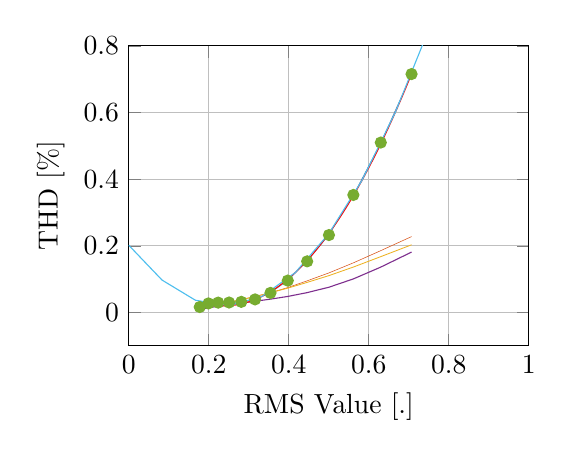
\begin{tikzpicture}

\begin{axis}[%
width=2.0in,
height=1.5in,
at={(0.758in,0.481in)},
scale only axis,
xmin=0,
xmax=1,
xmajorgrids,
ymajorgrids,
xlabel={RMS Value [.]},
ymin=-0.1,
ymax=0.8,
ylabel={THD [\%]},
axis background/.style={fill=white},
legend style={legend cell align=left,align=left,draw=white!15!black},
every axis legend/.code={\let\addlegendentry\relax}
]
\addplot [color=mycolor1,solid,line width=0.1pt]
  table[row sep=crcr]{%
0.177615489572042	0.0163567296283457\\
0.19928785706971	0.0271228498066899\\
0.223604653350506	0.0295265736362988\\
0.250888547527061	0.0298520327299892\\
0.281501580298378	0.0318157817378405\\
0.315849968009946	0.0391286280303762\\
0.354389492897844	0.0586725764661003\\
0.397631551042096	0.0955722177415252\\
0.446149938281945	0.153347756985553\\
0.500588464138024	0.232232513156654\\
0.561669494773539	0.352505293778709\\
0.630203538354371	0.509770381870535\\
0.7071	0.715231671701207\\
};
\addlegendentry{40 Hz};

\addplot [color=mycolor2,solid,line width=0.2pt]
  table[row sep=crcr]{%
0.177615489572042	0.00748774730570476\\
0.19928785706971	0.0153035671279335\\
0.223604653350506	0.022778438205278\\
0.250888547527061	0.0303755860732631\\
0.281501580298378	0.0384896658031986\\
0.315849968009946	0.0476176661950662\\
0.354389492897844	0.0593353716542332\\
0.397631551042096	0.0746431233492528\\
0.446149938281945	0.0949112661371481\\
0.500588464138024	0.118710744596914\\
0.561669494773539	0.148875681657143\\
0.630203538354371	0.185504424909765\\
0.7071	0.227605769742239\\
};
\addlegendentry{50 Hz};

\addplot [color=mycolor3,solid,line width=0.3pt]
  table[row sep=crcr]{%
0.177615489572042	0.00884021907907391\\
0.19928785706971	0.0165743647525293\\
0.223604653350506	0.023091022129994\\
0.250888547527061	0.0306649228571181\\
0.281501580298378	0.0385657951020248\\
0.315849968009946	0.0479698193164831\\
0.354389492897844	0.0590669359293038\\
0.397631551042096	0.0729628760419199\\
0.446149938281945	0.0902481232755839\\
0.500588464138024	0.11056705446719\\
0.561669494773539	0.136257732306928\\
0.630203538354371	0.167542090050669\\
0.7071	0.202980644764779\\
};
\addlegendentry{60 Hz};

\addplot [color=mycolor4,solid,line width=0.4pt]
  table[row sep=crcr]{%
0.177615489572042	0.00811932313650455\\
0.19928785706971	0.014192608330503\\
0.223604653350506	0.0186179033589375\\
0.250888547527061	0.0233081985950591\\
0.281501580298378	0.0282419431433296\\
0.315849968009946	0.0336357383017595\\
0.354389492897844	0.039950552358776\\
0.397631551042096	0.048062858042871\\
0.446149938281945	0.0595555164140927\\
0.500588464138024	0.0757427140043165\\
0.561669494773539	0.10068902861268\\
0.630203538354371	0.136128716401325\\
0.7071	0.181114060834515\\
};
\addlegendentry{70 Hz};

\addplot [color=mycolor5,only marks,mark=*,mark options={solid}]
  table[row sep=crcr]{%
0.177615489572042	0.0163567296283457\\
0.19928785706971	0.0271228498066899\\
0.223604653350506	0.0295265736362988\\
0.250888547527061	0.0298520327299892\\
0.281501580298378	0.0318157817378405\\
0.315849968009946	0.0391286280303762\\
0.354389492897844	0.0586725764661003\\
0.397631551042096	0.0955722177415252\\
0.446149938281945	0.153347756985553\\
0.500588464138024	0.232232513156654\\
0.561669494773539	0.352505293778709\\
0.630203538354371	0.509770381870535\\
0.7071	0.715231671701207\\
};
\addlegendentry{data};

\addplot [color=red,solid]
  table[row sep=crcr]{%
0.177615489572042	0.0321199059208065\\
0.17814497408247	0.0319137469247087\\
0.178674458592898	0.0317093693983951\\
0.179203943103326	0.0315067733418658\\
0.179733427613754	0.0313059587551206\\
0.180262912124182	0.0311069256381596\\
0.18079239663461	0.0309096739909829\\
0.181321881145038	0.0307142038135903\\
0.181851365655466	0.0305205151059819\\
0.182380850165894	0.0303286078681578\\
0.182910334676322	0.0301384821001178\\
0.18343981918675	0.0299501378018621\\
0.183969303697178	0.0297635749733905\\
0.184498788207606	0.0295787936147032\\
0.185028272718034	0.0293957937258\\
0.185557757228462	0.0292145753066811\\
0.18608724173889	0.0290351383573464\\
0.186616726249318	0.0288574828777958\\
0.187146210759746	0.0286816088680295\\
0.187675695270174	0.0285075163280474\\
0.188205179780602	0.0283352052578494\\
0.18873466429103	0.0281646756574357\\
0.189264148801457	0.0279959275268062\\
0.189793633311885	0.0278289608659608\\
0.190323117822313	0.0276637756748997\\
0.190852602332741	0.0275003719536228\\
0.191382086843169	0.0273387497021301\\
0.191911571353597	0.0271789089204216\\
0.192441055864025	0.0270208496084973\\
0.192970540374453	0.0268645717663572\\
0.193500024884881	0.0267100753940013\\
0.194029509395309	0.0265573604914296\\
0.194558993905737	0.0264064270586421\\
0.195088478416165	0.0262572750956388\\
0.195617962926593	0.0261099046024197\\
0.196147447437021	0.0259643155789848\\
0.196676931947449	0.0258205080253341\\
0.197206416457877	0.0256784819414676\\
0.197735900968305	0.0255382373273854\\
0.198265385478733	0.0253997741830873\\
0.198794869989161	0.0252630925085734\\
0.19928785706971	0.0251374338246403\\
0.199324354499589	0.0251281923038437\\
0.199853839010017	0.0249950735688983\\
0.200383323520445	0.024863736303737\\
0.200912808030873	0.0247341805083599\\
0.201442292541301	0.0246064061827671\\
0.201971777051728	0.0244804133269584\\
0.202501261562156	0.024356201940934\\
0.203030746072584	0.0242337720246937\\
0.203560230583012	0.0241131235782377\\
0.20408971509344	0.0239942566015658\\
0.204619199603868	0.0238771710946782\\
0.205148684114296	0.0237618670575747\\
0.205678168624724	0.0236483444902555\\
0.206207653135152	0.0235366033927205\\
0.20673713764558	0.0234266437649696\\
0.207266622156008	0.023318465607003\\
0.207796106666436	0.0232120689188206\\
0.208325591176864	0.0231074537004224\\
0.208855075687292	0.0230046199518084\\
0.20938456019772	0.0229035676729785\\
0.209914044708148	0.0228042968639329\\
0.210443529218576	0.0227068075246715\\
0.210973013729004	0.0226110996551943\\
0.211502498239432	0.0225171732555013\\
0.21203198274986	0.0224250283255925\\
0.212561467260288	0.0223346648654679\\
0.213090951770716	0.0222460828751275\\
0.213620436281144	0.0221592823545713\\
0.214149920791571	0.0220742633037993\\
0.214679405301999	0.0219910257228115\\
0.215208889812427	0.0219095696116079\\
0.215738374322855	0.0218298949701885\\
0.216267858833283	0.0217520017985534\\
0.216797343343711	0.0216758900967023\\
0.217326827854139	0.0216015598646356\\
0.217856312364567	0.021529011102353\\
0.218385796874995	0.0214582438098546\\
0.218915281385423	0.0213892579871405\\
0.219444765895851	0.0213220536342105\\
0.219974250406279	0.0212566307510647\\
0.220503734916707	0.0211929893377032\\
0.221033219427135	0.0211311293941258\\
0.221562703937563	0.0210710509203327\\
0.222092188447991	0.0210127539163237\\
0.222621672958419	0.020956238382099\\
0.223151157468847	0.0209015043176584\\
0.223604653350506	0.020856041693208\\
0.223680641979275	0.0208485517230021\\
0.224210126489703	0.0207973805981299\\
0.224739611000131	0.020747990943042\\
0.225269095510559	0.0207003827577383\\
0.225798580020987	0.0206545560422188\\
0.226328064531414	0.0206105107964834\\
0.226857549041842	0.0205682470205323\\
0.22738703355227	0.0205277647143654\\
0.227916518062698	0.0204890638779827\\
0.228446002573126	0.0204521445113841\\
0.228975487083554	0.0204170066145698\\
0.229504971593982	0.0203836501875397\\
0.23003445610441	0.0203520752302938\\
0.230563940614838	0.0203222817428321\\
0.231093425125266	0.0202942697251546\\
0.231622909635694	0.0202680391772613\\
0.232152394146122	0.0202435900991522\\
0.23268187865655	0.0202209224908273\\
0.233211363166978	0.0202000363522866\\
0.233740847677406	0.0201809316835301\\
0.234270332187834	0.0201636084845578\\
0.234799816698262	0.0201480667553698\\
0.23532930120869	0.0201343064959659\\
0.235858785719118	0.0201223277063462\\
0.236388270229546	0.0201121303865107\\
0.236917754739974	0.0201037145364594\\
0.237447239250402	0.0200970801561924\\
0.23797672376083	0.0200922272457095\\
0.238506208271258	0.0200891558050108\\
0.239035692781685	0.0200878658340964\\
0.239565177292113	0.0200883573329661\\
0.240094661802541	0.0200906303016201\\
0.240624146312969	0.0200946847400582\\
0.241153630823397	0.0201005206482806\\
0.241683115333825	0.0201081380262871\\
0.242212599844253	0.0201175368740779\\
0.242742084354681	0.0201287171916528\\
0.243271568865109	0.020141678979012\\
0.243801053375537	0.0201564222361554\\
0.244330537885965	0.0201729469630829\\
0.244860022396393	0.0201912531597947\\
0.245389506906821	0.0202113408262907\\
0.245918991417249	0.0202332099625708\\
0.246448475927677	0.0202568605686352\\
0.246977960438105	0.0202822926444838\\
0.247507444948533	0.0203095061901166\\
0.248036929458961	0.0203385012055336\\
0.248566413969389	0.0203692776907347\\
0.249095898479817	0.0204018356457201\\
0.249625382990245	0.0204361750704897\\
0.250154867500673	0.0204722959650435\\
0.250684352011101	0.0205101983293815\\
0.250888547527061	0.0205252913496377\\
0.251213836521529	0.0205498821635037\\
0.251743321031956	0.0205913474674101\\
0.252272805542384	0.0206345942411007\\
0.252802290052812	0.0206796224845756\\
0.25333177456324	0.0207264321978346\\
0.253861259073668	0.0207750233808778\\
0.254390743584096	0.0208253960337052\\
0.254920228094524	0.0208775501563168\\
0.255449712604952	0.0209314857487126\\
0.25597919711538	0.0209872028108927\\
0.256508681625808	0.0210447013428569\\
0.257038166136236	0.0211039813446053\\
0.257567650646664	0.021165042816138\\
0.258097135157092	0.0212278857574548\\
0.25862661966752	0.0212925101685559\\
0.259156104177948	0.0213589160494411\\
0.259685588688376	0.0214271034001105\\
0.260215073198804	0.0214970722205642\\
0.260744557709232	0.0215688225108021\\
0.26127404221966	0.0216423542708241\\
0.261803526730088	0.0217176675006304\\
0.262333011240516	0.0217947622002208\\
0.262862495750944	0.0218736383695955\\
0.263391980261372	0.0219542960087544\\
0.263921464771799	0.0220367351176974\\
0.264450949282227	0.0221209556964247\\
0.264980433792655	0.0222069577449362\\
0.265509918303083	0.0222947412632318\\
0.266039402813511	0.0223843062513117\\
0.266568887323939	0.0224756527091758\\
0.267098371834367	0.0225687806368241\\
0.267627856344795	0.0226636900342566\\
0.268157340855223	0.0227603809014733\\
0.268686825365651	0.0228588532384742\\
0.269216309876079	0.0229591070452593\\
0.269745794386507	0.0230611423218286\\
0.270275278896935	0.0231649590681821\\
0.270804763407363	0.0232705572843198\\
0.271334247917791	0.0233779369702417\\
0.271863732428219	0.0234870981259478\\
0.272393216938647	0.0235980407514381\\
0.272922701449075	0.0237107648467126\\
0.273452185959503	0.0238252704117713\\
0.273981670469931	0.0239415574466143\\
0.274511154980359	0.0240596259512414\\
0.275040639490787	0.0241794759256527\\
0.275570124001215	0.0243011073698483\\
0.276099608511643	0.024424520283828\\
0.27662909302207	0.0245497146675919\\
0.277158577532498	0.0246766905211401\\
0.277688062042926	0.0248054478444724\\
0.278217546553354	0.0249359866375889\\
0.278747031063782	0.0250683069004897\\
0.27927651557421	0.0252024086331746\\
0.279806000084638	0.0253382918356438\\
0.280335484595066	0.0254759565078972\\
0.280864969105494	0.0256154026499347\\
0.281394453615922	0.0257566302617565\\
0.281501580298378	0.0257854204768052\\
0.28192393812635	0.0258996393433625\\
0.282453422636778	0.0260444298947526\\
0.282982907147206	0.026191001915927\\
0.283512391657634	0.0263393554068855\\
0.284041876168062	0.0264894903676283\\
0.28457136067849	0.0266414067981553\\
0.285100845188918	0.0267951046984665\\
0.285630329699346	0.0269505840685619\\
0.286159814209774	0.0271078449084415\\
0.286689298720202	0.0272668872181052\\
0.28721878323063	0.0274277109975532\\
0.287748267741058	0.0275903162467854\\
0.288277752251486	0.0277547029658018\\
0.288807236761913	0.0279208711546024\\
0.289336721272341	0.0280888208131873\\
0.289866205782769	0.0282585519415562\\
0.290395690293197	0.0284300645397094\\
0.290925174803625	0.0286033586076468\\
0.291454659314053	0.0287784341453685\\
0.291984143824481	0.0289552911528743\\
0.292513628334909	0.0291339296301643\\
0.293043112845337	0.0293143495772385\\
0.293572597355765	0.029496550994097\\
0.294102081866193	0.0296805338807396\\
0.294631566376621	0.0298662982371664\\
0.295161050887049	0.0300538440633775\\
0.295690535397477	0.0302431713593727\\
0.296220019907905	0.0304342801251521\\
0.296749504418333	0.0306271703607157\\
0.297278988928761	0.0308218420660636\\
0.297808473439189	0.0310182952411956\\
0.298337957949617	0.0312165298861119\\
0.298867442460045	0.0314165460008124\\
0.299396926970473	0.031618343585297\\
0.299926411480901	0.0318219226395659\\
0.300455895991329	0.0320272831636189\\
0.300985380501756	0.0322344251574562\\
0.301514865012184	0.0324433486210777\\
0.302044349522612	0.0326540535544833\\
0.30257383403304	0.0328665399576732\\
0.303103318543468	0.0330808078306473\\
0.303632803053896	0.0332968571734056\\
0.304162287564324	0.033514687985948\\
0.304691772074752	0.0337343002682747\\
0.30522125658518	0.0339556940203856\\
0.305750741095608	0.0341788692422807\\
0.306280225606036	0.03440382593396\\
0.306809710116464	0.0346305640954235\\
0.307339194626892	0.0348590837266712\\
0.30786867913732	0.0350893848277031\\
0.308398163647748	0.0353214673985192\\
0.308927648158176	0.0355553314391195\\
0.309457132668604	0.035790976949504\\
0.309986617179032	0.0360284039296727\\
0.31051610168946	0.0362676123796257\\
0.311045586199888	0.0365086022993628\\
0.311575070710316	0.0367513736888841\\
0.312104555220744	0.0369959265481896\\
0.312634039731172	0.0372422608772793\\
0.3131635242416	0.0374903766761533\\
0.313693008752027	0.0377402739448114\\
0.314222493262455	0.0379919526832537\\
0.314751977772883	0.0382454128914803\\
0.315281462283311	0.038500654569491\\
0.315810946793739	0.038757677717286\\
0.315849968009946	0.0387766899351983\\
0.316340431304167	0.0390164823348651\\
0.316869915814595	0.0392770684222284\\
0.317399400325023	0.039539435979376\\
0.317928884835451	0.0398035850063077\\
0.318458369345879	0.0400695155030237\\
0.318987853856307	0.0403372274695239\\
0.319517338366735	0.0406067209058082\\
0.320046822877163	0.0408779958118768\\
0.320576307387591	0.0411510521877295\\
0.321105791898019	0.0414258900333666\\
0.321635276408447	0.0417025093487877\\
0.322164760918875	0.0419809101339931\\
0.322694245429303	0.0422610923889826\\
0.323223729939731	0.0425430561137564\\
0.323753214450159	0.0428268013083144\\
0.324282698960587	0.0431123279726566\\
0.324812183471015	0.043399636106783\\
0.325341667981443	0.0436887257106936\\
0.32587115249187	0.0439795967843883\\
0.326400637002298	0.0442722493278674\\
0.326930121512726	0.0445666833411306\\
0.327459606023154	0.044862898824178\\
0.327989090533582	0.0451608957770096\\
0.32851857504401	0.0454606741996254\\
0.329048059554438	0.0457622340920254\\
0.329577544064866	0.0460655754542096\\
0.330107028575294	0.0463706982861781\\
0.330636513085722	0.0466776025879307\\
0.33116599759615	0.0469862883594675\\
0.331695482106578	0.0472967556007885\\
0.332224966617006	0.0476090043118937\\
0.332754451127434	0.0479230344927832\\
0.333283935637862	0.0482388461434568\\
0.33381342014829	0.0485564392639147\\
0.334342904658718	0.0488758138541567\\
0.334872389169146	0.049196969914183\\
0.335401873679574	0.0495199074439934\\
0.335931358190002	0.049844626443588\\
0.33646084270043	0.0501711269129669\\
0.336990327210858	0.05049940885213\\
0.337519811721286	0.0508294722610772\\
0.338049296231714	0.0511613171398086\\
0.338578780742141	0.0514949434883243\\
0.339108265252569	0.0518303513066242\\
0.339637749762997	0.0521675405947083\\
0.340167234273425	0.0525065113525765\\
0.340696718783853	0.052847263580229\\
0.341226203294281	0.0531897972776657\\
0.341755687804709	0.0535341124448865\\
0.342285172315137	0.0538802090818916\\
0.342814656825565	0.0542280871886809\\
0.343344141335993	0.0545777467652545\\
0.343873625846421	0.0549291878116121\\
0.344403110356849	0.055282410327754\\
0.344932594867277	0.0556374143136801\\
0.345462079377705	0.0559941997693904\\
0.345991563888133	0.0563527666948849\\
0.346521048398561	0.0567131150901636\\
0.347050532908989	0.0570752449552265\\
0.347580017419417	0.0574391562900736\\
0.348109501929845	0.0578048490947049\\
0.348638986440273	0.0581723233691205\\
0.349168470950701	0.0585415791133202\\
0.349697955461129	0.0589126163273041\\
0.350227439971557	0.0592854350110721\\
0.350756924481984	0.0596600351646245\\
0.351286408992412	0.0600364167879611\\
0.35181589350284	0.0604145798810818\\
0.352345378013268	0.0607945244439868\\
0.352874862523696	0.0611762504766759\\
0.353404347034124	0.0615597579791491\\
0.353933831544552	0.0619450469514068\\
0.354389492897844	0.0622780433832734\\
0.35446331605498	0.0623321173934484\\
0.354992800565408	0.0627209693052745\\
0.355522285075836	0.0631116026868846\\
0.356051769586264	0.063504017538279\\
0.356581254096692	0.0638982138594575\\
0.35711073860712	0.0642941916504202\\
0.357640223117548	0.0646919509111672\\
0.358169707627976	0.0650914916416984\\
0.358699192138404	0.0654928138420138\\
0.359228676648832	0.0658959175121133\\
0.35975816115926	0.066300802651997\\
0.360287645669688	0.0667074692616651\\
0.360817130180116	0.0671159173411172\\
0.361346614690544	0.0675261468903536\\
0.361876099200972	0.0679381579093742\\
0.3624055837114	0.0683519503981789\\
0.362935068221828	0.068767524356768\\
0.363464552732255	0.0691848797851412\\
0.363994037242683	0.0696040166832986\\
0.364523521753111	0.0700249350512402\\
0.365053006263539	0.070447634888966\\
0.365582490773967	0.070872116196476\\
0.366111975284395	0.0712983789737702\\
0.366641459794823	0.0717264232208486\\
0.367170944305251	0.0721562489377113\\
0.367700428815679	0.072587856124358\\
0.368229913326107	0.073021244780789\\
0.368759397836535	0.0734564149070042\\
0.369288882346963	0.0738933665030037\\
0.369818366857391	0.0743320995687874\\
0.370347851367819	0.0747726141043552\\
0.370877335878247	0.0752149101097072\\
0.371406820388675	0.0756589875848434\\
0.371936304899103	0.0761048465297638\\
0.372465789409531	0.0765524869444685\\
0.372995273919959	0.0770019088289573\\
0.373524758430387	0.0774531121832304\\
0.374054242940815	0.0779060970072877\\
0.374583727451243	0.0783608633011291\\
0.375113211961671	0.0788174110647548\\
0.375642696472098	0.0792757402981646\\
0.376172180982526	0.0797358510013587\\
0.376701665492954	0.080197743174337\\
0.377231150003382	0.0806614168170994\\
0.37776063451381	0.0811268719296461\\
0.378290119024238	0.0815941085119769\\
0.378819603534666	0.082063126564092\\
0.379349088045094	0.0825339260859913\\
0.379878572555522	0.0830065070776748\\
0.38040805706595	0.0834808695391425\\
0.380937541576378	0.0839570134703943\\
0.381467026086806	0.0844349388714304\\
0.381996510597234	0.0849146457422507\\
0.382525995107662	0.0853961340828552\\
0.38305547961809	0.0858794038932439\\
0.383584964128518	0.0863644551734167\\
0.384114448638946	0.0868512879233739\\
0.384643933149374	0.0873399021431152\\
0.385173417659802	0.0878302978326407\\
0.38570290217023	0.0883224749919505\\
0.386232386680658	0.0888164336210444\\
0.386761871191086	0.0893121737199225\\
0.387291355701514	0.0898096952885848\\
0.387820840211942	0.0903089983270313\\
0.388350324722369	0.090810082835262\\
0.388879809232797	0.091312948813277\\
0.389409293743225	0.0918175962610761\\
0.389938778253653	0.0923240251786594\\
0.390468262764081	0.0928322355660269\\
0.390997747274509	0.0933422274231787\\
0.391527231784937	0.0938540007501146\\
0.392056716295365	0.0943675555468348\\
0.392586200805793	0.0948828918133391\\
0.393115685316221	0.0954000095496277\\
0.393645169826649	0.0959189087557004\\
0.394174654337077	0.0964395894315574\\
0.394704138847505	0.0969620515771986\\
0.395233623357933	0.097486295192624\\
0.395763107868361	0.0980123202778334\\
0.396292592378789	0.0985401268328272\\
0.396822076889217	0.0990697148576052\\
0.397351561399645	0.0996010843521674\\
0.397631551042096	0.0998827908581341\\
0.397881045910073	0.100134235316514\\
0.398410530420501	0.100669167750644\\
0.398940014930929	0.101205881654559\\
0.399469499441357	0.101744377028258\\
0.399998983951785	0.102284653871741\\
0.400528468462212	0.102826712185009\\
0.40105795297264	0.10337055196806\\
0.401587437483068	0.103916173220896\\
0.402116921993496	0.104463575943516\\
0.402646406503924	0.10501276013592\\
0.403175891014352	0.105563725798109\\
0.40370537552478	0.106116472930081\\
0.404234860035208	0.106671001531838\\
0.404764344545636	0.107227311603379\\
0.405293829056064	0.107785403144704\\
0.405823313566492	0.108345276155814\\
0.40635279807692	0.108906930636707\\
0.406882282587348	0.109470366587385\\
0.407411767097776	0.110035584007847\\
0.407941251608204	0.110602582898093\\
0.408470736118632	0.111171363258124\\
0.40900022062906	0.111741925087938\\
0.409529705139488	0.112314268387537\\
0.410059189649916	0.11288839315692\\
0.410588674160344	0.113464299396088\\
0.411118158670772	0.114041987105039\\
0.4116476431812	0.114621456283775\\
0.412177127691628	0.115202706932295\\
0.412706612202056	0.115785739050599\\
0.413236096712484	0.116370552638687\\
0.413765581222911	0.116957147696559\\
0.414295065733339	0.117545524224216\\
0.414824550243767	0.118135682221657\\
0.415354034754195	0.118727621688882\\
0.415883519264623	0.119321342625891\\
0.416413003775051	0.119916845032685\\
0.416942488285479	0.120514128909262\\
0.417471972795907	0.121113194255624\\
0.418001457306335	0.12171404107177\\
0.418530941816763	0.122316669357701\\
0.419060426327191	0.122921079113415\\
0.419589910837619	0.123527270338914\\
0.420119395348047	0.124135243034197\\
0.420648879858475	0.124744997199264\\
0.421178364368903	0.125356532834115\\
0.421707848879331	0.12596984993875\\
0.422237333389759	0.12658494851317\\
0.422766817900187	0.127201828557374\\
0.423296302410615	0.127820490071362\\
0.423825786921043	0.128440933055135\\
0.424355271431471	0.129063157508691\\
0.424884755941899	0.129687163432032\\
0.425414240452327	0.130312950825157\\
0.425943724962754	0.130940519688066\\
0.426473209473182	0.131569870020759\\
0.42700269398361	0.132201001823237\\
0.427532178494038	0.132833915095498\\
0.428061663004466	0.133468609837544\\
0.428591147514894	0.134105086049374\\
0.429120632025322	0.134743343730989\\
0.42965011653575	0.135383382882387\\
0.430179601046178	0.13602520350357\\
0.430709085556606	0.136668805594537\\
0.431238570067034	0.137314189155288\\
0.431768054577462	0.137961354185824\\
0.43229753908789	0.138610300686143\\
0.432827023598318	0.139261028656247\\
0.433356508108746	0.139913538096135\\
0.433885992619174	0.140567829005807\\
0.434415477129602	0.141223901385263\\
0.43494496164003	0.141881755234504\\
0.435474446150458	0.142541390553529\\
0.436003930660886	0.143202807342338\\
0.436533415171314	0.143866005600931\\
0.437062899681742	0.144530985329308\\
0.43759238419217	0.14519774652747\\
0.438121868702598	0.145866289195416\\
0.438651353213025	0.146536613333145\\
0.439180837723453	0.14720871894066\\
0.439710322233881	0.147882606017958\\
0.440239806744309	0.148558274565041\\
0.440769291254737	0.149235724581908\\
0.441298775765165	0.149914956068559\\
0.441828260275593	0.150595969024994\\
0.442357744786021	0.151278763451213\\
0.442887229296449	0.151963339347217\\
0.443416713806877	0.152649696713005\\
0.443946198317305	0.153337835548577\\
0.444475682827733	0.154027755853933\\
0.445005167338161	0.154719457629073\\
0.445534651848589	0.155412940873998\\
0.446064136359017	0.156108205588707\\
0.446149938281945	0.156221039599642\\
0.446593620869445	0.1568052517732\\
0.447123105379873	0.157504079427477\\
0.447652589890301	0.158204688551538\\
0.448182074400729	0.158907079145384\\
0.448711558911157	0.159611251209014\\
0.449241043421585	0.160317204742428\\
0.449770527932013	0.161024939745626\\
0.450300012442441	0.161734456218609\\
0.450829496952868	0.162445754161375\\
0.451358981463296	0.163158833573926\\
0.451888465973724	0.163873694456261\\
0.452417950484152	0.164590336808381\\
0.45294743499458	0.165308760630284\\
0.453476919505008	0.166028965921972\\
0.454006404015436	0.166750952683444\\
0.454535888525864	0.167474720914699\\
0.455065373036292	0.16820027061574\\
0.45559485754672	0.168927601786564\\
0.456124342057148	0.169656714427173\\
0.456653826567576	0.170387608537566\\
0.457183311078004	0.171120284117743\\
0.457712795588432	0.171854741167704\\
0.45824228009886	0.17259097968745\\
0.458771764609288	0.173328999676979\\
0.459301249119716	0.174068801136293\\
0.459830733630144	0.174810384065391\\
0.460360218140572	0.175553748464274\\
0.460889702651	0.17629889433294\\
0.461419187161428	0.177045821671391\\
0.461948671671856	0.177794530479626\\
0.462478156182284	0.178545020757645\\
0.463007640692712	0.179297292505448\\
0.463537125203139	0.180051345723036\\
0.464066609713567	0.180807180410408\\
0.464596094223995	0.181564796567564\\
0.465125578734423	0.182324194194504\\
0.465655063244851	0.183085373291228\\
0.466184547755279	0.183848333857736\\
0.466714032265707	0.184613075894029\\
0.467243516776135	0.185379599400106\\
0.467773001286563	0.186147904375967\\
0.468302485796991	0.186917990821613\\
0.468831970307419	0.187689858737042\\
0.469361454817847	0.188463508122256\\
0.469890939328275	0.189238938977254\\
0.470420423838703	0.190016151302036\\
0.470949908349131	0.190795145096602\\
0.471479392859559	0.191575920360953\\
0.472008877369987	0.192358477095088\\
0.472538361880415	0.193142815299007\\
0.473067846390843	0.19392893497271\\
0.473597330901271	0.194716836116197\\
0.474126815411699	0.195506518729469\\
0.474656299922127	0.196297982812525\\
0.475185784432555	0.197091228365365\\
0.475715268942982	0.197886255387989\\
0.47624475345341	0.198683063880397\\
0.476774237963838	0.19948165384259\\
0.477303722474266	0.200282025274567\\
0.477833206984694	0.201084178176328\\
0.478362691495122	0.201888112547873\\
0.47889217600555	0.202693828389202\\
0.479421660515978	0.203501325700316\\
0.479951145026406	0.204310604481214\\
0.480480629536834	0.205121664731896\\
0.481010114047262	0.205934506452362\\
0.48153959855769	0.206749129642612\\
0.482069083068118	0.207565534302647\\
0.482598567578546	0.208383720432466\\
0.483128052088974	0.209203688032069\\
0.483657536599402	0.210025437101456\\
0.48418702110983	0.210848967640627\\
0.484716505620258	0.211674279649583\\
0.485245990130686	0.212501373128323\\
0.485775474641114	0.213330248076847\\
0.486304959151542	0.214160904495155\\
0.48683444366197	0.214993342383247\\
0.487363928172397	0.215827561741124\\
0.487893412682825	0.216663562568785\\
0.488422897193253	0.21750134486623\\
0.488952381703681	0.218340908633459\\
0.489481866214109	0.219182253870473\\
0.490011350724537	0.22002538057727\\
0.490540835234965	0.220870288753852\\
0.491070319745393	0.221716978400218\\
0.491599804255821	0.222565449516369\\
0.492129288766249	0.223415702102303\\
0.492658773276677	0.224267736158022\\
0.493188257787105	0.225121551683525\\
0.493717742297533	0.225977148678812\\
0.494247226807961	0.226834527143883\\
0.494776711318389	0.227693687078739\\
0.495306195828817	0.228554628483378\\
0.495835680339245	0.229417351357802\\
0.496365164849673	0.23028185570201\\
0.496894649360101	0.231148141516002\\
0.497424133870529	0.232016208799779\\
0.497953618380957	0.23288605755334\\
0.498483102891385	0.233757687776685\\
0.499012587401813	0.234631099469814\\
0.499542071912241	0.235506292632727\\
0.500071556422669	0.236383267265425\\
0.500588464138024	0.237241129703034\\
0.500601040933096	0.237262023367906\\
0.501130525443524	0.238142560940172\\
0.501660009953952	0.239024879982222\\
0.50218949446438	0.239908980494056\\
0.502718978974808	0.240794862475675\\
0.503248463485236	0.241682525927078\\
0.503777947995664	0.242571970848265\\
0.504307432506092	0.243463197239236\\
0.50483691701652	0.244356205099991\\
0.505366401526948	0.245250994430531\\
0.505895886037376	0.246147565230854\\
0.506425370547804	0.247045917500962\\
0.506954855058232	0.247946051240854\\
0.50748433956866	0.248847966450531\\
0.508013824079088	0.249751663129991\\
0.508543308589516	0.250657141279236\\
0.509072793099944	0.251564400898265\\
0.509602277610372	0.252473441987078\\
0.5101317621208	0.253384264545676\\
0.510661246631228	0.254296868574057\\
0.511190731141656	0.255211254072223\\
0.511720215652084	0.256127421040173\\
0.512249700162511	0.257045369477907\\
0.512779184672939	0.257965099385426\\
0.513308669183367	0.258886610762728\\
0.513838153693795	0.259809903609815\\
0.514367638204223	0.260734977926686\\
0.514897122714651	0.261661833713341\\
0.515426607225079	0.262590470969781\\
0.515956091735507	0.263520889696004\\
0.516485576245935	0.264453089892012\\
0.517015060756363	0.265387071557804\\
0.517544545266791	0.26632283469338\\
0.518074029777219	0.26726037929874\\
0.518603514287647	0.268199705373885\\
0.519132998798075	0.269140812918814\\
0.519662483308503	0.270083701933527\\
0.520191967818931	0.271028372418024\\
0.520721452329359	0.271974824372306\\
0.521250936839787	0.272923057796371\\
0.521780421350215	0.273873072690221\\
0.522309905860643	0.274824869053855\\
0.522839390371071	0.275778446887273\\
0.523368874881499	0.276733806190476\\
0.523898359391927	0.277690946963462\\
0.524427843902355	0.278649869206233\\
0.524957328412783	0.279610572918788\\
0.52548681292321	0.280573058101127\\
0.526016297433638	0.281537324753251\\
0.526545781944066	0.282503372875159\\
0.527075266454494	0.28347120246685\\
0.527604750964922	0.284440813528327\\
0.52813423547535	0.285412206059587\\
0.528663719985778	0.286385380060631\\
0.529193204496206	0.28736033553146\\
0.529722689006634	0.288337072472073\\
0.530252173517062	0.28931559088247\\
0.53078165802749	0.290295890762651\\
0.531311142537918	0.291277972112617\\
0.531840627048346	0.292261834932366\\
0.532370111558774	0.2932474792219\\
0.532899596069202	0.294234904981218\\
0.53342908057963	0.29522411221032\\
0.533958565090058	0.296215100909207\\
0.534488049600486	0.297207871077878\\
0.535017534110914	0.298202422716333\\
0.535547018621342	0.299198755824572\\
0.53607650313177	0.300196870402595\\
0.536605987642198	0.301196766450403\\
0.537135472152626	0.302198443967994\\
0.537664956663053	0.30320190295537\\
0.538194441173481	0.30420714341253\\
0.538723925683909	0.305214165339475\\
0.539253410194337	0.306222968736203\\
0.539782894704765	0.307233553602716\\
0.540312379215193	0.308245919939013\\
0.540841863725621	0.309260067745094\\
0.541371348236049	0.310275997020959\\
0.541900832746477	0.311293707766609\\
0.542430317256905	0.312313199982043\\
0.542959801767333	0.31333447366726\\
0.543489286277761	0.314357528822263\\
0.544018770788189	0.315382365447049\\
0.544548255298617	0.316408983541619\\
0.545077739809045	0.317437383105974\\
0.545607224319473	0.318467564140113\\
0.546136708829901	0.319499526644036\\
0.546666193340329	0.320533270617744\\
0.547195677850757	0.321568796061235\\
0.547725162361185	0.322606102974511\\
0.548254646871613	0.323645191357571\\
0.548784131382041	0.324686061210415\\
0.549313615892469	0.325728712533043\\
0.549843100402897	0.326773145325456\\
0.550372584913325	0.327819359587653\\
0.550902069423752	0.328867355319634\\
0.55143155393418	0.329917132521399\\
0.551961038444608	0.330968691192948\\
0.552490522955036	0.332022031334282\\
0.553020007465464	0.3330771529454\\
0.553549491975892	0.334134056026302\\
0.55407897648632	0.335192740576988\\
0.554608460996748	0.336253206597458\\
0.555137945507176	0.337315454087713\\
0.555667430017604	0.338379483047752\\
0.556196914528032	0.339445293477575\\
0.55672639903846	0.340512885377182\\
0.557255883548888	0.341582258746573\\
0.557785368059316	0.342653413585749\\
0.558314852569744	0.343726349894709\\
0.558844337080172	0.344801067673453\\
0.5593738215906	0.345877566921981\\
0.559903306101028	0.346955847640294\\
0.560432790611456	0.34803590982839\\
0.560962275121884	0.349117753486271\\
0.561491759632312	0.350201378613936\\
0.561669494773539	0.350565524719587\\
0.56202124414274	0.351286785211385\\
0.562550728653167	0.352373973278619\\
0.563080213163595	0.353462942815636\\
0.563609697674023	0.354553693822438\\
0.564139182184451	0.355646226299024\\
0.564668666694879	0.356740540245395\\
0.565198151205307	0.357836635661549\\
0.565727635715735	0.358934512547488\\
0.566257120226163	0.36003417090321\\
0.566786604736591	0.361135610728718\\
0.567316089247019	0.362238832024009\\
0.567845573757447	0.363343834789084\\
0.568375058267875	0.364450619023944\\
0.568904542778303	0.365559184728588\\
0.569434027288731	0.366669531903016\\
0.569963511799159	0.367781660547228\\
0.570492996309587	0.368895570661225\\
0.571022480820015	0.370011262245005\\
0.571551965330443	0.37112873529857\\
0.572081449840871	0.372247989821919\\
0.572610934351299	0.373369025815053\\
0.573140418861727	0.37449184327797\\
0.573669903372155	0.375616442210672\\
0.574199387882583	0.376742822613158\\
0.574728872393011	0.377870984485428\\
0.575258356903439	0.379000927827482\\
0.575787841413866	0.380132652639321\\
0.576317325924294	0.381266158920943\\
0.576846810434722	0.38240144667235\\
0.57737629494515	0.383538515893541\\
0.577905779455578	0.384677366584517\\
0.578435263966006	0.385817998745276\\
0.578964748476434	0.38696041237582\\
0.579494232986862	0.388104607476148\\
0.58002371749729	0.38925058404626\\
0.580553202007718	0.390398342086156\\
0.581082686518146	0.391547881595837\\
0.581612171028574	0.392699202575302\\
0.582141655539002	0.39385230502455\\
0.58267114004943	0.395007188943584\\
0.583200624559858	0.396163854332401\\
0.583730109070286	0.397322301191003\\
0.584259593580714	0.398482529519388\\
0.584789078091142	0.399644539317558\\
0.58531856260157	0.400808330585513\\
0.585848047111998	0.401973903323251\\
0.586377531622426	0.403141257530773\\
0.586907016132854	0.40431039320808\\
0.587436500643281	0.405481310355171\\
0.587965985153709	0.406654008972046\\
0.588495469664137	0.407828489058706\\
0.589024954174565	0.409004750615149\\
0.589554438684993	0.410182793641377\\
0.590083923195421	0.411362618137389\\
0.590613407705849	0.412544224103185\\
0.591142892216277	0.413727611538766\\
0.591672376726705	0.41491278044413\\
0.592201861237133	0.416099730819279\\
0.592731345747561	0.417288462664212\\
0.593260830257989	0.418478975978929\\
0.593790314768417	0.419671270763431\\
0.594319799278845	0.420865347017716\\
0.594849283789273	0.422061204741786\\
0.595378768299701	0.42325884393564\\
0.595908252810129	0.424458264599278\\
0.596437737320557	0.425659466732701\\
0.596967221830985	0.426862450335907\\
0.597496706341413	0.428067215408898\\
0.598026190851841	0.429273761951673\\
0.598555675362269	0.430482089964233\\
0.599085159872697	0.431692199446576\\
0.599614644383125	0.432904090398703\\
0.600144128893553	0.434117762820615\\
0.60067361340398	0.435333216712311\\
0.601203097914408	0.436550452073792\\
0.601732582424836	0.437769468905056\\
0.602262066935264	0.438990267206105\\
0.602791551445692	0.440212846976938\\
0.60332103595612	0.441437208217555\\
0.603850520466548	0.442663350927956\\
0.604380004976976	0.443891275108141\\
0.604909489487404	0.445120980758111\\
0.605438973997832	0.446352467877865\\
0.60596845850826	0.447585736467403\\
0.606497943018688	0.448820786526725\\
0.607027427529116	0.450057618055832\\
0.607556912039544	0.451296231054722\\
0.608086396549972	0.452536625523397\\
0.6086158810604	0.453778801461856\\
0.609145365570828	0.4550227588701\\
0.609674850081256	0.456268497748127\\
0.610204334591684	0.457516018095939\\
0.610733819102112	0.458765319913535\\
0.61126330361254	0.460016403200915\\
0.611792788122968	0.461269267958079\\
0.612322272633395	0.462523914185027\\
0.612851757143823	0.46378034188176\\
0.613381241654251	0.465038551048277\\
0.613910726164679	0.466298541684578\\
0.614440210675107	0.467560313790664\\
0.614969695185535	0.468823867366533\\
0.615499179695963	0.470089202412187\\
0.616028664206391	0.471356318927625\\
0.616558148716819	0.472625216912847\\
0.617087633227247	0.473895896367853\\
0.617617117737675	0.475168357292644\\
0.618146602248103	0.476442599687219\\
0.618676086758531	0.477718623551578\\
0.619205571268959	0.478996428885721\\
0.619735055779387	0.480276015689648\\
0.620264540289815	0.481557383963359\\
0.620794024800243	0.482840533706855\\
0.621323509310671	0.484125464920135\\
0.621852993821099	0.485412177603199\\
0.622382478331527	0.486700671756048\\
0.622911962841955	0.48799094737868\\
0.623441447352383	0.489283004471097\\
0.623970931862811	0.490576843033298\\
0.624500416373239	0.491872463065283\\
0.625029900883667	0.493169864567053\\
0.625559385394094	0.494469047538606\\
0.626088869904522	0.495770011979944\\
0.62661835441495	0.497072757891066\\
0.627147838925378	0.498377285271972\\
0.627677323435806	0.499683594122663\\
0.628206807946234	0.500991684443137\\
0.628736292456662	0.502301556233396\\
0.62926577696709	0.503613209493439\\
0.629795261477518	0.504926644223266\\
0.630203538354371	0.505940628773543\\
0.630324745987946	0.506241860422877\\
0.630854230498374	0.507558858092273\\
0.631383715008802	0.508877637231453\\
0.63191319951923	0.510198197840417\\
0.632442684029658	0.511520539919165\\
0.632972168540086	0.512844663467698\\
0.633501653050514	0.514170568486014\\
0.634031137560942	0.515498254974115\\
0.63456062207137	0.516827722932\\
0.635090106581798	0.518158972359669\\
0.635619591092226	0.519492003257123\\
0.636149075602654	0.52082681562436\\
0.636678560113082	0.522163409461382\\
0.63720804462351	0.523501784768188\\
0.637737529133937	0.524841941544778\\
0.638267013644365	0.526183879791153\\
0.638796498154793	0.527527599507311\\
0.639325982665221	0.528873100693254\\
0.639855467175649	0.530220383348981\\
0.640384951686077	0.531569447474493\\
0.640914436196505	0.532920293069788\\
0.641443920706933	0.534272920134868\\
0.641973405217361	0.535627328669732\\
0.642502889727789	0.53698351867438\\
0.643032374238217	0.538341490148812\\
0.643561858748645	0.539701243093028\\
0.644091343259073	0.541062777507029\\
0.644620827769501	0.542426093390814\\
0.645150312279929	0.543791190744383\\
0.645679796790357	0.545158069567736\\
0.646209281300785	0.546526729860874\\
0.646738765811213	0.547897171623795\\
0.647268250321641	0.549269394856501\\
0.647797734832069	0.550643399558991\\
0.648327219342497	0.552019185731266\\
0.648856703852925	0.553396753373324\\
0.649386188363352	0.554776102485167\\
0.64991567287378	0.556157233066794\\
0.650445157384208	0.557540145118205\\
0.650974641894636	0.5589248386394\\
0.651504126405064	0.56031131363038\\
0.652033610915492	0.561699570091143\\
0.65256309542592	0.563089608021691\\
0.653092579936348	0.564481427422023\\
0.653622064446776	0.56587502829214\\
0.654151548957204	0.56727041063204\\
0.654681033467632	0.568667574441725\\
0.65521051797806	0.570066519721194\\
0.655740002488488	0.571467246470447\\
0.656269486998916	0.572869754689484\\
0.656798971509344	0.574274044378306\\
0.657328456019772	0.575680115536912\\
0.6578579405302	0.577087968165302\\
0.658387425040628	0.578497602263476\\
0.658916909551056	0.579909017831434\\
0.659446394061484	0.581322214869177\\
0.659975878571912	0.582737193376703\\
0.66050536308234	0.584153953354015\\
0.661034847592768	0.585572494801109\\
0.661564332103196	0.586992817717989\\
0.662093816613624	0.588414922104653\\
0.662623301124051	0.5898388079611\\
0.663152785634479	0.591264475287332\\
0.663682270144907	0.592691924083348\\
0.664211754655335	0.594121154349149\\
0.664741239165763	0.595552166084733\\
0.665270723676191	0.596984959290102\\
0.665800208186619	0.598419533965255\\
0.666329692697047	0.599855890110192\\
0.666859177207475	0.601294027724914\\
0.667388661717903	0.602733946809419\\
0.667918146228331	0.604175647363709\\
0.668447630738759	0.605619129387783\\
0.668977115249187	0.607064392881641\\
0.669506599759615	0.608511437845284\\
0.670036084270043	0.60996026427871\\
0.670565568780471	0.611410872181921\\
0.671095053290899	0.612863261554916\\
0.671624537801327	0.614317432397695\\
0.672154022311755	0.615773384710259\\
0.672683506822183	0.617231118492606\\
0.673212991332611	0.618690633744738\\
0.673742475843039	0.620151930466654\\
0.674271960353466	0.621615008658354\\
0.674801444863894	0.623079868319839\\
0.675330929374322	0.624546509451108\\
0.67586041388475	0.62601493205216\\
0.676389898395178	0.627485136122998\\
0.676919382905606	0.628957121663619\\
0.677448867416034	0.630430888674024\\
0.677978351926462	0.631906437154214\\
0.67850783643689	0.633383767104188\\
0.679037320947318	0.634862878523946\\
0.679566805457746	0.636343771413488\\
0.680096289968174	0.637826445772814\\
0.680625774478602	0.639310901601925\\
0.68115525898903	0.64079713890082\\
0.681684743499458	0.642285157669499\\
0.682214228009886	0.643774957907962\\
0.682743712520314	0.64526653961621\\
0.683273197030742	0.646759902794241\\
0.68380268154117	0.648255047442057\\
0.684332166051598	0.649751973559657\\
0.684861650562026	0.651250681147042\\
0.685391135072454	0.65275117020421\\
0.685920619582882	0.654253440731163\\
0.68645010409331	0.6557574927279\\
0.686979588603738	0.657263326194421\\
0.687509073114166	0.658770941130726\\
0.688038557624593	0.660280337536816\\
0.688568042135021	0.661791515412689\\
0.689097526645449	0.663304474758347\\
0.689627011155877	0.664819215573789\\
0.690156495666305	0.666335737859016\\
0.690685980176733	0.667854041614026\\
0.691215464687161	0.669374126838821\\
0.691744949197589	0.6708959935334\\
0.692274433708017	0.672419641697763\\
0.692803918218445	0.673945071331911\\
0.693333402728873	0.675472282435842\\
0.693862887239301	0.677001275009558\\
0.694392371749729	0.678532049053057\\
0.694921856260157	0.680064604566342\\
0.695451340770585	0.68159894154941\\
0.695980825281013	0.683135060002262\\
0.696510309791441	0.6846729599249\\
0.697039794301869	0.68621264131732\\
0.697569278812297	0.687754104179526\\
0.698098763322725	0.689297348511515\\
0.698628247833153	0.690842374313288\\
0.699157732343581	0.692389181584846\\
0.699687216854008	0.693937770326188\\
0.700216701364436	0.695488140537314\\
0.700746185874864	0.697040292218224\\
0.701275670385292	0.698594225368919\\
0.70180515489572	0.700149939989398\\
0.702334639406148	0.701707436079661\\
0.702864123916576	0.703266713639708\\
0.703393608427004	0.704827772669539\\
0.703923092937432	0.706390613169155\\
0.70445257744786	0.707955235138555\\
0.704982061958288	0.709521638577739\\
0.705511546468716	0.711089823486707\\
0.706041030979144	0.712659789865459\\
0.706570515489572	0.714231537713996\\
0.7071	0.715805067032317\\
};
\addlegendentry{fitted curve};

\addplot [color=mycolor6,solid,forget plot]
  table[row sep=crcr]{%
0	0.2018\\
0.0833333333333333	0.0971958333333334\\
0.166666666666667	0.0367166666666667\\
0.25	0.0203625\\
0.333333333333333	0.0481333333333334\\
0.416666666666667	0.120029166666667\\
0.5	0.23605\\
0.583333333333333	0.396195833333334\\
0.666666666666667	0.600466666666667\\
0.75	0.8488625\\
0.833333333333333	1.14138333333333\\
0.916666666666667	1.47802916666667\\
1	1.8588\\
};

\end{axis}
\end{tikzpicture}%
    \caption{Band 1 from 33 Hz to 66 Hz}
    \label{fig:Band1Model}
\end{subfigure}
\begin{subfigure}[t]{0.45\textwidth}
    \centering
    \tikzsetnextfilename{Band2Model}
    % This file was created by matlab2tikz.
%
%The latest updates can be retrieved from
%  http://www.mathworks.com/matlabcentral/fileexchange/22022-matlab2tikz-matlab2tikz
%where you can also make suggestions and rate matlab2tikz.
%
\definecolor{mycolor1}{rgb}{0.00000,0.44700,0.74100}%
\definecolor{mycolor2}{rgb}{0.85000,0.32500,0.09800}%
\definecolor{mycolor3}{rgb}{0.92900,0.69400,0.12500}%
\definecolor{mycolor4}{rgb}{0.49400,0.18400,0.55600}%
\definecolor{mycolor5}{rgb}{0.46600,0.67400,0.18800}%
\definecolor{mycolor6}{rgb}{0.30100,0.74500,0.93300}%
\definecolor{mycolor7}{rgb}{0.63500,0.07800,0.18400}%
%
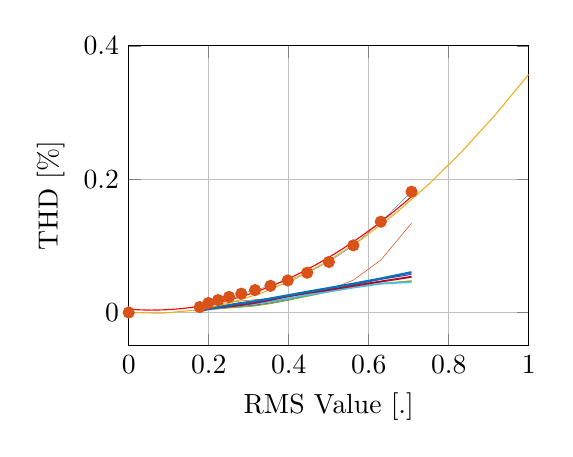
\begin{tikzpicture}

\begin{axis}[%
width=2.0in,
height=1.5in,
at={(0.758in,0.481in)},
scale only axis,
xmin=0,
xmax=1,
xlabel={RMS Value [.]},
xmajorgrids,
ymajorgrids,
ymin=-0.05,
ymax=0.4,
ylabel={THD [\%]},
axis background/.style={fill=white},
legend style={legend cell align=left,align=left,draw=white!15!black},
every axis legend/.code={\let\addlegendentry\relax}
]
\addplot [color=mycolor1,solid,line width=0.1pt]
  table[row sep=crcr]{%
0.177615489572042	0.00811932313650455\\
0.19928785706971	0.014192608330503\\
0.223604653350506	0.0186179033589375\\
0.250888547527061	0.0233081985950591\\
0.281501580298378	0.0282419431433296\\
0.315849968009946	0.0336357383017595\\
0.354389492897844	0.039950552358776\\
0.397631551042096	0.048062858042871\\
0.446149938281945	0.0595555164140927\\
0.500588464138024	0.0757427140043165\\
0.561669494773539	0.10068902861268\\
0.630203538354371	0.136128716401325\\
0.7071	0.181114060834515\\
};
\addlegendentry{70 Hz};

\addplot [color=mycolor2,solid,line width=0.2pt]
  table[row sep=crcr]{%
0.177615489572042	0.00601154860816139\\
0.19928785706971	0.0098879437959762\\
0.223604653350506	0.0126330055422494\\
0.250888547527061	0.014884171411781\\
0.281501580298378	0.0173583467164611\\
0.315849968009946	0.0191413444724763\\
0.354389492897844	0.0209350588236994\\
0.397631551042096	0.0235817896837536\\
0.446149938281945	0.0277682193800434\\
0.500588464138024	0.0342671618365613\\
0.561669494773539	0.0485594111797584\\
0.630203538354371	0.0786446986291868\\
0.7071	0.133857908068269\\
};
\addlegendentry{80 Hz};

\addplot [color=mycolor3,solid,line width=0.3pt]
  table[row sep=crcr]{%
0.177615489572042	0.00447101681012402\\
0.19928785706971	0.00700755812042933\\
0.223604653350506	0.00880565715116074\\
0.250888547527061	0.010618292192637\\
0.281501580298378	0.0118000308654507\\
0.315849968009946	0.013577634035287\\
0.354389492897844	0.0163690864600391\\
0.397631551042096	0.0207058019494006\\
0.446149938281945	0.0266735218981882\\
0.500588464138024	0.0326922480882402\\
0.561669494773539	0.0382714980652651\\
0.630203538354371	0.0430592328848868\\
0.7071	0.0477747309008454\\
};
\addlegendentry{90 Hz};

\addplot [color=mycolor4,solid,line width=0.4pt]
  table[row sep=crcr]{%
0.177615489572042	0.00349055655077128\\
0.19928785706971	0.00508975400374632\\
0.223604653350506	0.00658007477389928\\
0.250888547527061	0.00785609087948696\\
0.281501580298378	0.00908642292722114\\
0.315849968009946	0.0109843851383131\\
0.354389492897844	0.0140540796658637\\
0.397631551042096	0.0190858954650593\\
0.446149938281945	0.0258775368046788\\
0.500588464138024	0.0333603769063016\\
0.561669494773539	0.0415530336794478\\
0.630203538354371	0.049806033906725\\
0.7071	0.0571464792180492\\
};
\addlegendentry{100 Hz};

\addplot [color=mycolor5,solid]
  table[row sep=crcr]{%
0.177615489572042	0.0026027606361005\\
0.19928785706971	0.00430329207290324\\
0.223604653350506	0.0055778957415307\\
0.250888547527061	0.00691988381058196\\
0.281501580298378	0.00822387696359113\\
0.315849968009946	0.0100497005449854\\
0.354389492897844	0.0135081747721002\\
0.397631551042096	0.0184083736548551\\
0.446149938281945	0.024341093050581\\
0.500588464138024	0.0310557148113978\\
0.561669494773539	0.0377010961332953\\
0.630203538354371	0.0435695313363341\\
0.7071	0.0470812455639205\\
};
\addlegendentry{110 Hz};

\addplot [color=mycolor6,solid,line width=0.6pt]
  table[row sep=crcr]{%
0.177615489572042	0.00244987294960432\\
0.19928785706971	0.00447857718449775\\
0.223604653350506	0.00641889786489436\\
0.250888547527061	0.00835675606765249\\
0.281501580298378	0.0102150886948135\\
0.315849968009946	0.0131065774680663\\
0.354389492897844	0.0163560550598713\\
0.397631551042096	0.0207027133693768\\
0.446149938281945	0.026242508358693\\
0.500588464138024	0.0312657884114461\\
0.561669494773539	0.0373060037764674\\
0.630203538354371	0.0430287541943271\\
0.7071	0.0455167986104014\\
};
\addlegendentry{120 Hz};

\addplot [color=mycolor7,solid,line width=0.7pt]
  table[row sep=crcr]{%
0.177615489572042	0.00259404686172193\\
0.19928785706971	0.00522345471826321\\
0.223604653350506	0.00731141304967469\\
0.250888547527061	0.00899082838595957\\
0.281501580298378	0.0112662967455765\\
0.315849968009946	0.0144806295888977\\
0.354389492897844	0.0187753224915562\\
0.397631551042096	0.0241074837339837\\
0.446149938281945	0.0293583611499775\\
0.500588464138024	0.0338657496627046\\
0.561669494773539	0.0399846958342867\\
0.630203538354371	0.0463998022623881\\
0.7071	0.053447319391773\\
};
\addlegendentry{130 Hz};

\addplot [color=mycolor1,solid,line width=0.8pt]
  table[row sep=crcr]{%
0.177615489572042	0.00281550869189747\\
0.19928785706971	0.00579102233850549\\
0.223604653350506	0.00833724920963191\\
0.250888547527061	0.011089449640169\\
0.281501580298378	0.0140535489887201\\
0.315849968009946	0.0168712055985728\\
0.354389492897844	0.020978580147255\\
0.397631551042096	0.0256346127296753\\
0.446149938281945	0.0309903755999393\\
0.500588464138024	0.0366268475572401\\
0.561669494773539	0.0431598178212298\\
0.630203538354371	0.0508665295530352\\
0.7071	0.060327374914144\\
};
\addlegendentry{140 Hz};

\addplot [color=mycolor2,only marks,mark=*,mark options={solid}]
  table[row sep=crcr]{%
0	0\\
0.177615489572042	0.00811932313650455\\
0.19928785706971	0.014192608330503\\
0.223604653350506	0.0186179033589375\\
0.250888547527061	0.0233081985950591\\
0.281501580298378	0.0282419431433296\\
0.315849968009946	0.0336357383017595\\
0.354389492897844	0.039950552358776\\
0.397631551042096	0.048062858042871\\
0.446149938281945	0.0595555164140927\\
0.500588464138024	0.0757427140043165\\
0.561669494773539	0.10068902861268\\
0.630203538354371	0.136128716401325\\
0.7071	0.181114060834515\\
};
\addlegendentry{data};

\addplot [color=red,solid]
  table[row sep=crcr]{%
0	0.00494850749548683\\
0.0007071	0.00491597162390794\\
0.0014142	0.004883839232955\\
0.0021213	0.00485211032262802\\
0.0028284	0.004820784892927\\
0.0035355	0.00478986294385193\\
0.0042426	0.00475934447540282\\
0.0049497	0.00472922948757966\\
0.0056568	0.00469951798038247\\
0.0063639	0.00467020995381123\\
0.007071	0.00464130540786595\\
0.0077781	0.00461280434254662\\
0.0084852	0.00458470675785325\\
0.0091923	0.00455701265378584\\
0.0098994	0.00452972203034438\\
0.0106065	0.00450283488752889\\
0.0113136	0.00447635122533934\\
0.0120207	0.00445027104377576\\
0.0127278	0.00442459434283813\\
0.0134349	0.00439932112252646\\
0.014142	0.00437445138284075\\
0.0148491	0.00434998512378099\\
0.0155562	0.00432592234534719\\
0.0162633	0.00430226304753935\\
0.0169704	0.00427900723035746\\
0.0176775	0.00425615489380153\\
0.0183846	0.00423370603787156\\
0.0190917	0.00421166066256754\\
0.0197988	0.00419001876788948\\
0.0205059	0.00416878035383738\\
0.021213	0.00414794542041124\\
0.0219201	0.00412751396761105\\
0.0226272	0.00410748599543682\\
0.0233343	0.00408786150388854\\
0.0240414	0.00406864049296622\\
0.0247485	0.00404982296266986\\
0.0254556	0.00403140891299946\\
0.0261627	0.00401339834395501\\
0.0268698	0.00399579125553652\\
0.0275769	0.00397858764774399\\
0.028284	0.00396178752057741\\
0.0289911	0.00394539087403679\\
0.0296982	0.00392939770812213\\
0.0304053	0.00391380802283343\\
0.0311124	0.00389862181817068\\
0.0318195	0.00388383909413389\\
0.0325266	0.00386945985072305\\
0.0332337	0.00385548408793817\\
0.0339408	0.00384191180577925\\
0.0346479	0.00382874300424629\\
0.035355	0.00381597768333928\\
0.0360621	0.00380361584305823\\
0.0367692	0.00379165748340314\\
0.0374763	0.003780102604374\\
0.0381834	0.00376895120597082\\
0.0388905	0.0037582032881936\\
0.0395976	0.00374785885104233\\
0.0403047	0.00373791789451702\\
0.0410118	0.00372838041861767\\
0.0417189	0.00371924642334427\\
0.042426	0.00371051590869684\\
0.0431331	0.00370218887467535\\
0.0438402	0.00369426532127983\\
0.0445473	0.00368674524851026\\
0.0452544	0.00367962865636665\\
0.0459615	0.003672915544849\\
0.0466686	0.0036666059139573\\
0.0473757	0.00366069976369156\\
0.0480828	0.00365519709405178\\
0.0487899	0.00365009790503795\\
0.049497	0.00364540219665008\\
0.0502041	0.00364110996888817\\
0.0509112	0.00363722122175221\\
0.0516183	0.00363373595524221\\
0.0523254	0.00363065416935817\\
0.0530325	0.00362797586410008\\
0.0537396	0.00362570103946796\\
0.0544467	0.00362382969546178\\
0.0551538	0.00362236183208157\\
0.0558609	0.00362129744932731\\
0.056568	0.00362063654719901\\
0.0572751	0.00362037912569667\\
0.0579822	0.00362052518482028\\
0.0586893	0.00362107472456985\\
0.0593964	0.00362202774494538\\
0.0601035	0.00362338424594686\\
0.0608106	0.0036251442275743\\
0.0615177	0.0036273076898277\\
0.0622248	0.00362987463270705\\
0.0629319	0.00363284505621236\\
0.063639	0.00363621896034363\\
0.0643461	0.00363999634510086\\
0.0650532	0.00364417721048404\\
0.0657603	0.00364876155649318\\
0.0664674	0.00365374938312827\\
0.0671745	0.00365914069038933\\
0.0678816	0.00366493547827634\\
0.0685887	0.0036711337467893\\
0.0692958	0.00367773549592822\\
0.0700029	0.0036847407256931\\
0.07071	0.00369214943608394\\
0.0714171	0.00369996162710074\\
0.0721242	0.00370817729874349\\
0.0728313	0.00371679645101219\\
0.0735384	0.00372581908390686\\
0.0742455	0.00373524519742748\\
0.0749526	0.00374507479157406\\
0.0756597	0.00375530786634659\\
0.0763668	0.00376594442174508\\
0.0770739	0.00377698445776953\\
0.077781	0.00378842797441994\\
0.0784881	0.0038002749716963\\
0.0791952	0.00381252544959862\\
0.0799023	0.0038251794081269\\
0.0806094	0.00383823684728113\\
0.0813165	0.00385169776706132\\
0.0820236	0.00386556216746747\\
0.0827307	0.00387983004849957\\
0.0834378	0.00389450141015763\\
0.0841449	0.00390957625244165\\
0.084852	0.00392505457535163\\
0.0855591	0.00394093637888756\\
0.0862662	0.00395722166304945\\
0.0869733	0.00397391042783729\\
0.0876804	0.00399100267325109\\
0.0883875	0.00400849839929085\\
0.0890946	0.00402639760595657\\
0.0898017	0.00404470029324824\\
0.0905088	0.00406340646116587\\
0.0912159	0.00408251610970946\\
0.091923	0.004102029238879\\
0.0926301	0.0041219458486745\\
0.0933372	0.00414226593909596\\
0.0940443	0.00416298951014337\\
0.0947514	0.00418411656181674\\
0.0954585	0.00420564709411607\\
0.0961656	0.00422758110704136\\
0.0968727	0.0042499186005926\\
0.0975798	0.0042726595747698\\
0.0982869	0.00429580402957295\\
0.098994	0.00431935196500207\\
0.0997011	0.00434330338105713\\
0.1004082	0.00436765827773816\\
0.1011153	0.00439241665504514\\
0.1018224	0.00441757851297808\\
0.1025295	0.00444314385153698\\
0.1032366	0.00446911267072183\\
0.1039437	0.00449548497053264\\
0.1046508	0.00452226075096941\\
0.1053579	0.00454944001203214\\
0.106065	0.00457702275372082\\
0.1067721	0.00460500897603545\\
0.1074792	0.00463339867897605\\
0.1081863	0.0046621918625426\\
0.1088934	0.00469138852673511\\
0.1096005	0.00472098867155358\\
0.1103076	0.004750992296998\\
0.1110147	0.00478139940306838\\
0.1117218	0.00481220998976471\\
0.1124289	0.00484342405708701\\
0.113136	0.00487504160503526\\
0.1138431	0.00490706263360946\\
0.1145502	0.00493948714280963\\
0.1152573	0.00497231513263575\\
0.1159644	0.00500554660308783\\
0.1166715	0.00503918155416586\\
0.1173786	0.00507321998586985\\
0.1180857	0.0051076618981998\\
0.1187928	0.00514250729115571\\
0.1194999	0.00517775616473757\\
0.120207	0.00521340851894539\\
0.1209141	0.00524946435377916\\
0.1216212	0.00528592366923889\\
0.1223283	0.00532278646532458\\
0.1230354	0.00536005274203623\\
0.1237425	0.00539772249937384\\
0.1244496	0.00543579573733739\\
0.1251567	0.00547427245592691\\
0.1258638	0.00551315265514239\\
0.1265709	0.00555243633498382\\
0.127278	0.0055921234954512\\
0.1279851	0.00563221413654455\\
0.1286922	0.00567270825826385\\
0.1293993	0.00571360586060911\\
0.1301064	0.00575490694358033\\
0.1308135	0.0057966115071775\\
0.1315206	0.00583871955140063\\
0.1322277	0.00588123107624971\\
0.1329348	0.00592414608172475\\
0.1336419	0.00596746456782575\\
0.134349	0.00601118653455271\\
0.1350561	0.00605531198190563\\
0.1357632	0.00609984090988449\\
0.1364703	0.00614477331848932\\
0.1371774	0.00619010920772011\\
0.1378845	0.00623584857757685\\
0.1385916	0.00628199142805955\\
0.1392987	0.0063285377591682\\
0.1400058	0.00637548757090281\\
0.1407129	0.00642284086326338\\
0.14142	0.00647059763624991\\
0.1421271	0.00651875788986239\\
0.1428342	0.00656732162410083\\
0.1435413	0.00661628883896523\\
0.1442484	0.00666565953445558\\
0.1449555	0.00671543371057189\\
0.1456626	0.00676561136731415\\
0.1463697	0.00681619250468238\\
0.1470768	0.00686717712267656\\
0.1477839	0.00691856522129669\\
0.148491	0.00697035680054279\\
0.1491981	0.00702255186041484\\
0.1499052	0.00707515040091285\\
0.1506123	0.00712815242203681\\
0.1513194	0.00718155792378674\\
0.1520265	0.00723536690616262\\
0.1527336	0.00728957936916445\\
0.1534407	0.00734419531279224\\
0.1541478	0.00739921473704599\\
0.1548549	0.0074546376419257\\
0.155562	0.00751046402743136\\
0.1562691	0.00756669389356298\\
0.1569762	0.00762332724032056\\
0.1576833	0.00768036406770409\\
0.1583904	0.00773780437571358\\
0.1590975	0.00779564816434903\\
0.1598046	0.00785389543361044\\
0.1605117	0.0079125461834978\\
0.1612188	0.00797160041401112\\
0.1619259	0.00803105812515039\\
0.162633	0.00809091931691562\\
0.1633401	0.00815118398930681\\
0.1640472	0.00821185214232396\\
0.1647543	0.00827292377596706\\
0.1654614	0.00833439889023612\\
0.1661685	0.00839627748513114\\
0.1668756	0.00845855956065211\\
0.1675827	0.00852124511679904\\
0.1682898	0.00858433415357193\\
0.1689969	0.00864782667097077\\
0.169704	0.00871172266899557\\
0.1704111	0.00877602214764633\\
0.1711182	0.00884072510692304\\
0.1718253	0.00890583154682572\\
0.1725324	0.00897134146735435\\
0.1732395	0.00903725486850893\\
0.1739466	0.00910357175028947\\
0.1746537	0.00917029211269597\\
0.1753608	0.00923741595572843\\
0.1760679	0.00930494327938684\\
0.176775	0.00937287408367121\\
0.1774821	0.00944120836858154\\
0.177615489572042	0.00945414439951267\\
0.1781892	0.00950994613411782\\
0.1788963	0.00957908738028006\\
0.1796034	0.00964863210706826\\
0.1803105	0.00971858031448241\\
0.1810176	0.00978893200252252\\
0.1817247	0.00985968717118859\\
0.1824318	0.00993084582048062\\
0.1831389	0.0100024079503986\\
0.183846	0.0100743735609425\\
0.1845531	0.0101467426521124\\
0.1852602	0.0102195152239083\\
0.1859673	0.0102926912763301\\
0.1866744	0.0103662708093779\\
0.1873815	0.0104402538230516\\
0.1880886	0.0105146403173513\\
0.1887957	0.0105894302922769\\
0.1895028	0.0106646237478285\\
0.1902099	0.010740220684006\\
0.190917	0.0108162211008096\\
0.1916241	0.010892624998239\\
0.1923312	0.0109694323762944\\
0.1930383	0.0110466432349758\\
0.1937454	0.0111242575742832\\
0.1944525	0.0112022753942164\\
0.1951596	0.0112806966947757\\
0.1958667	0.0113595214759609\\
0.1965738	0.0114387497377721\\
0.1972809	0.0115183814802092\\
0.197988	0.0115984167032723\\
0.1986951	0.0116788554069613\\
0.19928785706971	0.0117465975069343\\
0.1994022	0.0117596975912763\\
0.2001093	0.0118409432562172\\
0.2008164	0.0119225924017841\\
0.2015235	0.012004645027977\\
0.2022306	0.0120871011347958\\
0.2029377	0.0121699607222406\\
0.2036448	0.0122532237903113\\
0.2043519	0.012336890339008\\
0.205059	0.0124209603683306\\
0.2057661	0.0125054338782793\\
0.2064732	0.0125903108688538\\
0.2071803	0.0126755913400543\\
0.2078874	0.0127612752918808\\
0.2085945	0.0128473627243332\\
0.2093016	0.0129338536374116\\
0.2100087	0.013020748031116\\
0.2107158	0.0131080459054463\\
0.2114229	0.0131957472604025\\
0.21213	0.0132838520959847\\
0.2128371	0.0133723604121929\\
0.2135442	0.013461272209027\\
0.2142513	0.0135505874864871\\
0.2149584	0.0136403062445732\\
0.2156655	0.0137304284832852\\
0.2163726	0.0138209542026231\\
0.2170797	0.013911883402587\\
0.2177868	0.0140032160831769\\
0.2184939	0.0140949522443927\\
0.219201	0.0141870918862345\\
0.2199081	0.0142796350087022\\
0.2206152	0.0143725816117959\\
0.2213223	0.0144659316955156\\
0.2220294	0.0145596852598612\\
0.2227365	0.0146538423048328\\
0.2234436	0.0147484028304303\\
0.223604653350506	0.0147699969200378\\
0.2241507	0.0148433668366538\\
0.2248578	0.0149387343235032\\
0.2255649	0.0150345052909786\\
0.226272	0.01513067973908\\
0.2269791	0.0152272576678073\\
0.2276862	0.0153242390771605\\
0.2283933	0.0154216239671397\\
0.2291004	0.0155194123377449\\
0.2298075	0.0156176041889761\\
0.2305146	0.0157161995208332\\
0.2312217	0.0158151983333162\\
0.2319288	0.0159146006264252\\
0.2326359	0.0160144064001602\\
0.233343	0.0161146156545211\\
0.2340501	0.016215228389508\\
0.2347572	0.0163162446051208\\
0.2354643	0.0164176643013596\\
0.2361714	0.0165194874782244\\
0.2368785	0.0166217141357151\\
0.2375856	0.0167243442738317\\
0.2382927	0.0168273778925743\\
0.2389998	0.0169308149919429\\
0.2397069	0.0170346555719374\\
0.240414	0.0171388996325579\\
0.2411211	0.0172435471738044\\
0.2418282	0.0173485981956768\\
0.2425353	0.0174540526981751\\
0.2432424	0.0175599106812995\\
0.2439495	0.0176661721450497\\
0.2446566	0.017772837089426\\
0.2453637	0.0178799055144282\\
0.2460708	0.0179873774200563\\
0.2467779	0.0180952528063104\\
0.247485	0.0182035316731905\\
0.2481921	0.0183122140206965\\
0.2488992	0.0184212998488284\\
0.2496063	0.0185307891575864\\
0.2503134	0.0186406819469703\\
0.250888547527061	0.0187303651239049\\
0.2510205	0.0187509782169801\\
0.2517276	0.0188616779676159\\
0.2524347	0.0189727811988777\\
0.2531418	0.0190842879107654\\
0.2538489	0.019196198103279\\
0.254556	0.0193085117764187\\
0.2552631	0.0194212289301843\\
0.2559702	0.0195343495645758\\
0.2566773	0.0196478736795933\\
0.2573844	0.0197618012752368\\
0.2580915	0.0198761323515062\\
0.2587986	0.0199908669084015\\
0.2595057	0.0201060049459229\\
0.2602128	0.0202215464640701\\
0.2609199	0.0203374914628434\\
0.261627	0.0204538399422426\\
0.2623341	0.0205705919022677\\
0.2630412	0.0206877473429188\\
0.2637483	0.0208053062641959\\
0.2644554	0.0209232686660989\\
0.2651625	0.0210416345486279\\
0.2658696	0.0211604039117828\\
0.2665767	0.0212795767555637\\
0.2672838	0.0213991530799706\\
0.2679909	0.0215191328850034\\
0.268698	0.0216395161706622\\
0.2694051	0.0217603029369469\\
0.2701122	0.0218814931838576\\
0.2708193	0.0220030869113942\\
0.2715264	0.0221250841195568\\
0.2722335	0.0222474848083453\\
0.2729406	0.0223702889777598\\
0.2736477	0.0224934966278003\\
0.2743548	0.0226171077584667\\
0.2750619	0.0227411223697591\\
0.275769	0.0228655404616774\\
0.2764761	0.0229903620342217\\
0.2771832	0.023115587087392\\
0.2778903	0.0232412156211882\\
0.2785974	0.0233672476356103\\
0.2793045	0.0234936831306585\\
0.2800116	0.0236205221063325\\
0.2807187	0.0237477645626326\\
0.2814258	0.0238754104995586\\
0.281501580298378	0.0238891143229855\\
0.2821329	0.0240034599171105\\
0.28284	0.0241319128152884\\
0.2835471	0.0242607691940923\\
0.2842542	0.0243900290535221\\
0.2849613	0.0245196923935779\\
0.2856684	0.0246497592142596\\
0.2863755	0.0247802295155673\\
0.2870826	0.0249111032975009\\
0.2877897	0.0250423805600605\\
0.2884968	0.0251740613032461\\
0.2892039	0.0253061455270576\\
0.289911	0.0254386332314951\\
0.2906181	0.0255715244165585\\
0.2913252	0.0257048190822479\\
0.2920323	0.0258385172285632\\
0.2927394	0.0259726188555045\\
0.2934465	0.0261071239630718\\
0.2941536	0.026242032551265\\
0.2948607	0.0263773446200841\\
0.2955678	0.0265130601695293\\
0.2962749	0.0266491791996004\\
0.296982	0.0267857017102974\\
0.2976891	0.0269226277016204\\
0.2983962	0.0270599571735694\\
0.2991033	0.0271976901261443\\
0.2998104	0.0273358265593451\\
0.3005175	0.027474366473172\\
0.3012246	0.0276133098676247\\
0.3019317	0.0277526567427035\\
0.3026388	0.0278924070984082\\
0.3033459	0.0280325609347388\\
0.304053	0.0281731182516954\\
0.3047601	0.028314079049278\\
0.3054672	0.0284554433274865\\
0.3061743	0.028597211086321\\
0.3068814	0.0287393823257814\\
0.3075885	0.0288819570458678\\
0.3082956	0.0290249352465802\\
0.3090027	0.0291683169279185\\
0.3097098	0.0293121020898828\\
0.3104169	0.029456290732473\\
0.311124	0.0296008828556892\\
0.3118311	0.0297458784595313\\
0.3125382	0.0298912775439994\\
0.3132453	0.0300370801090934\\
0.3139524	0.0301832861548134\\
0.3146595	0.0303298956811594\\
0.3153666	0.0304769086881313\\
0.315849968009946	0.0305776378067722\\
0.3160737	0.0306243251757292\\
0.3167808	0.030772145143953\\
0.3174879	0.0309203685928028\\
0.318195	0.0310689955222786\\
0.3189021	0.0312180259323803\\
0.3196092	0.0313674598231079\\
0.3203163	0.0315172971944615\\
0.3210234	0.0316675380464411\\
0.3217305	0.0318181823790466\\
0.3224376	0.0319692301922781\\
0.3231447	0.0321206814861356\\
0.3238518	0.032272536260619\\
0.3245589	0.0324247945157283\\
0.325266	0.0325774562514637\\
0.3259731	0.0327305214678249\\
0.3266802	0.0328839901648122\\
0.3273873	0.0330378623424254\\
0.3280944	0.0331921380006645\\
0.3288015	0.0333468171395296\\
0.3295086	0.0335018997590207\\
0.3302157	0.0336573858591377\\
0.3309228	0.0338132754398806\\
0.3316299	0.0339695685012496\\
0.332337	0.0341262650432445\\
0.3330441	0.0342833650658653\\
0.3337512	0.0344408685691121\\
0.3344583	0.0345987755529849\\
0.3351654	0.0347570860174836\\
0.3358725	0.0349157999626082\\
0.3365796	0.0350749173883588\\
0.3372867	0.0352344382947354\\
0.3379938	0.035394362681738\\
0.3387009	0.0355546905493665\\
0.339408	0.0357154218976209\\
0.3401151	0.0358765567265013\\
0.3408222	0.0360380950360077\\
0.3415293	0.03620003682614\\
0.3422364	0.0363623820968983\\
0.3429435	0.0365251308482825\\
0.3436506	0.0366882830802927\\
0.3443577	0.0368518387929289\\
0.3450648	0.037015797986191\\
0.3457719	0.0371801606600791\\
0.346479	0.0373449268145931\\
0.3471861	0.0375100964497331\\
0.3478932	0.037675669565499\\
0.3486003	0.0378416461618909\\
0.3493074	0.0380080262389088\\
0.3500145	0.0381748097965526\\
0.3507216	0.0383419968348223\\
0.3514287	0.038509587353718\\
0.3521358	0.0386775813532397\\
0.3528429	0.0388459788333874\\
0.35355	0.0390147797941609\\
0.3542571	0.0391839842355605\\
0.354389492897844	0.0392157098417403\\
0.3549642	0.039353592157586\\
0.3556713	0.0395236035602375\\
0.3563784	0.0396940184435149\\
0.3570855	0.0398648368074183\\
0.3577926	0.0400360586519476\\
0.3584997	0.0402076839771029\\
0.3592068	0.0403797127828841\\
0.3599139	0.0405521450692913\\
0.360621	0.0407249808363245\\
0.3613281	0.0408982200839836\\
0.3620352	0.0410718628122687\\
0.3627423	0.0412459090211797\\
0.3634494	0.0414203587107167\\
0.3641565	0.0415952118808796\\
0.3648636	0.0417704685316685\\
0.3655707	0.0419461286630834\\
0.3662778	0.0421221922751242\\
0.3669849	0.042298659367791\\
0.367692	0.0424755299410837\\
0.3683991	0.0426528039950024\\
0.3691062	0.042830481529547\\
0.3698133	0.0430085625447176\\
0.3705204	0.0431870470405142\\
0.3712275	0.0433659350169367\\
0.3719346	0.0435452264739852\\
0.3726417	0.0437249214116596\\
0.3733488	0.04390501982996\\
0.3740559	0.0440855217288863\\
0.374763	0.0442664271084386\\
0.3754701	0.0444477359686169\\
0.3761772	0.0446294483094211\\
0.3768843	0.0448115641308513\\
0.3775914	0.0449940834329074\\
0.3782985	0.0451770062155895\\
0.3790056	0.0453603324788975\\
0.3797127	0.0455440622228315\\
0.3804198	0.0457281954473914\\
0.3811269	0.0459127321525774\\
0.381834	0.0460976723383892\\
0.3825411	0.0462830160048271\\
0.3832482	0.0464687631518908\\
0.3839553	0.0466549137795806\\
0.3846624	0.0468414678878963\\
0.3853695	0.0470284254768379\\
0.3860766	0.0472157865464055\\
0.3867837	0.0474035510965991\\
0.3874908	0.0475917191274186\\
0.3881979	0.0477802906388641\\
0.388905	0.0479692656309355\\
0.3896121	0.0481586441036329\\
0.3903192	0.0483484260569563\\
0.3910263	0.0485386114909056\\
0.3917334	0.0487292004054808\\
0.3924405	0.0489201928006821\\
0.3931476	0.0491115886765092\\
0.3938547	0.0493033880329624\\
0.3945618	0.0494955908700415\\
0.3952689	0.0496881971877465\\
0.395976	0.0498812069860775\\
0.3966831	0.0500746202650345\\
0.3973902	0.0502684370246174\\
0.397631551042096	0.0503346839293542\\
0.3980973	0.0504626572648263\\
0.3988044	0.0506572809856611\\
0.3995115	0.0508523081871219\\
0.4002186	0.0510477388692086\\
0.4009257	0.0512435730319213\\
0.4016328	0.05143981067526\\
0.4023399	0.0516364517992246\\
0.403047	0.0518334964038152\\
0.4037541	0.0520309444890317\\
0.4044612	0.0522287960548742\\
0.4051683	0.0524270511013426\\
0.4058754	0.052625709628437\\
0.4065825	0.0528247716361574\\
0.4072896	0.0530242371245037\\
0.4079967	0.053224106093476\\
0.4087038	0.0534243785430742\\
0.4094109	0.0536250544732984\\
0.410118	0.0538261338841485\\
0.4108251	0.0540276167756246\\
0.4115322	0.0542295031477267\\
0.4122393	0.0544317930004547\\
0.4129464	0.0546344863338087\\
0.4136535	0.0548375831477886\\
0.4143606	0.0550410834423945\\
0.4150677	0.0552449872176263\\
0.4157748	0.0554492944734841\\
0.4164819	0.0556540052099679\\
0.417189	0.0558591194270776\\
0.4178961	0.0560646371248133\\
0.4186032	0.0562705583031749\\
0.4193103	0.0564768829621625\\
0.4200174	0.056683611101776\\
0.4207245	0.0568907427220155\\
0.4214316	0.057098277822881\\
0.4221387	0.0573062164043724\\
0.4228458	0.0575145584664897\\
0.4235529	0.0577233040092331\\
0.42426	0.0579324530326023\\
0.4249671	0.0581420055365976\\
0.4256742	0.0583519615212188\\
0.4263813	0.0585623209864659\\
0.4270884	0.058773083932339\\
0.4277955	0.0589842503588381\\
0.4285026	0.0591958202659631\\
0.4292097	0.0594077936537141\\
0.4299168	0.059620170522091\\
0.4306239	0.0598329508710939\\
0.431331	0.0600461347007228\\
0.4320381	0.0602597220109776\\
0.4327452	0.0604737128018583\\
0.4334523	0.0606881070733651\\
0.4341594	0.0609029048254977\\
0.4348665	0.0611181060582564\\
0.4355736	0.0613337107716409\\
0.4362807	0.0615497189656515\\
0.4369878	0.061766130640288\\
0.4376949	0.0619829457955505\\
0.438402	0.0622001644314389\\
0.4391091	0.0624177865479532\\
0.4398162	0.0626358121450936\\
0.4405233	0.0628542412228599\\
0.4412304	0.0630730737812521\\
0.4419375	0.0632923098202703\\
0.4426446	0.0635119493399145\\
0.4433517	0.0637319923401846\\
0.4440588	0.0639524388210807\\
0.4447659	0.0641732887826027\\
0.445473	0.0643945422247507\\
0.446149938281945	0.0646067360179922\\
0.4461801	0.0646161991475246\\
0.4468872	0.0648382595509245\\
0.4475943	0.0650607234349504\\
0.4483014	0.0652835907996022\\
0.4490085	0.06550686164488\\
0.4497156	0.0657305359707837\\
0.4504227	0.0659546137773134\\
0.4511298	0.066179095064469\\
0.4518369	0.0664039798322506\\
0.452544	0.0666292680806582\\
0.4532511	0.0668549598096917\\
0.4539582	0.0670810550193511\\
0.4546653	0.0673075537096366\\
0.4553724	0.067534455880548\\
0.4560795	0.0677617615320853\\
0.4567866	0.0679894706642486\\
0.4574937	0.0682175832770379\\
0.4582008	0.0684460993704531\\
0.4589079	0.0686750189444942\\
0.459615	0.0689043419991613\\
0.4603221	0.0691340685344544\\
0.4610292	0.0693641985503735\\
0.4617363	0.0695947320469185\\
0.4624434	0.0698256690240894\\
0.4631505	0.0700570094818863\\
0.4638576	0.0702887534203092\\
0.4645647	0.070520900839358\\
0.4652718	0.0707534517390328\\
0.4659789	0.0709864061193335\\
0.466686	0.0712197639802602\\
0.4673931	0.0714535253218129\\
0.4681002	0.0716876901439915\\
0.4688073	0.071922258446796\\
0.4695144	0.0721572302302266\\
0.4702215	0.072392605494283\\
0.4709286	0.0726283842389655\\
0.4716357	0.0728645664642739\\
0.4723428	0.0731011521702082\\
0.4730499	0.0733381413567685\\
0.473757	0.0735755340239548\\
0.4744641	0.073813330171767\\
0.4751712	0.0740515298002052\\
0.4758783	0.0742901329092693\\
0.4765854	0.0745291394989594\\
0.4772925	0.0747685495692755\\
0.4779996	0.0750083631202175\\
0.4787067	0.0752485801517854\\
0.4794138	0.0754892006639793\\
0.4801209	0.0757302246567992\\
0.480828	0.075971652130245\\
0.4815351	0.0762134830843168\\
0.4822422	0.0764557175190146\\
0.4829493	0.0766983554343383\\
0.4836564	0.0769413968302879\\
0.4843635	0.0771848417068635\\
0.4850706	0.0774286900640651\\
0.4857777	0.0776729419018926\\
0.4864848	0.0779175972203461\\
0.4871919	0.0781626560194256\\
0.487899	0.078408118299131\\
0.4886061	0.0786539840594623\\
0.4893132	0.0789002533004196\\
0.4900203	0.0791469260220029\\
0.4907274	0.0793940022242121\\
0.4914345	0.0796414819070473\\
0.4921416	0.0798893650705085\\
0.4928487	0.0801376517145956\\
0.4935558	0.0803863418393086\\
0.4942629	0.0806354354446476\\
0.49497	0.0808849325306126\\
0.4956771	0.0811348330972035\\
0.4963842	0.0813851371444204\\
0.4970913	0.0816358446722632\\
0.4977984	0.081886955680732\\
0.4985055	0.0821384701698268\\
0.4992126	0.0823903881395475\\
0.4999197	0.0826427095898942\\
0.500588464138024	0.082881722538597\\
0.5006268	0.0828954345208668\\
0.5013339	0.0831485629324654\\
0.502041	0.0834020948246899\\
0.5027481	0.0836560301975404\\
0.5034552	0.0839103690510168\\
0.5041623	0.0841651113851192\\
0.5048694	0.0844202571998476\\
0.5055765	0.0846758064952019\\
0.5062836	0.0849317592711822\\
0.5069907	0.0851881155277885\\
0.5076978	0.0854448752650206\\
0.5084049	0.0857020384828788\\
0.509112	0.0859596051813629\\
0.5098191	0.0862175753604729\\
0.5105262	0.086475949020209\\
0.5112333	0.086734726160571\\
0.5119404	0.0869939067815589\\
0.5126475	0.0872534908831728\\
0.5133546	0.0875134784654126\\
0.5140617	0.0877738695282784\\
0.5147688	0.0880346640717702\\
0.5154759	0.0882958620958879\\
0.516183	0.0885574636006316\\
0.5168901	0.0888194685860012\\
0.5175972	0.0890818770519968\\
0.5183043	0.0893446889986184\\
0.5190114	0.0896079044258659\\
0.5197185	0.0898715233337393\\
0.5204256	0.0901355457222388\\
0.5211327	0.0903999715913641\\
0.5218398	0.0906648009411154\\
0.5225469	0.0909300337714927\\
0.523254	0.091195670082496\\
0.5239611	0.0914617098741251\\
0.5246682	0.0917281531463803\\
0.5253753	0.0919949998992614\\
0.5260824	0.0922622501327685\\
0.5267895	0.0925299038469015\\
0.5274966	0.0927979610416605\\
0.5282037	0.0930664217170455\\
0.5289108	0.0933352858730564\\
0.5296179	0.0936045535096932\\
0.530325	0.093874224626956\\
0.5310321	0.0941442992248448\\
0.5317392	0.0944147773033595\\
0.5324463	0.0946856588625002\\
0.5331534	0.0949569439022668\\
0.5338605	0.0952286324226594\\
0.5345676	0.095500724423678\\
0.5352747	0.0957732199053225\\
0.5359818	0.096046118867593\\
0.5366889	0.0963194213104894\\
0.537396	0.0965931272340118\\
0.5381031	0.0968672366381601\\
0.5388102	0.0971417495229344\\
0.5395173	0.0974166658883347\\
0.5402244	0.0976919857343609\\
0.5409315	0.0979677090610131\\
0.5416386	0.0982438358682911\\
0.5423457	0.0985203661561953\\
0.5430528	0.0987972999247253\\
0.5437599	0.0990746371738813\\
0.544467	0.0993523779036632\\
0.5451741	0.0996305221140711\\
0.5458812	0.099909069805105\\
0.5465883	0.100188020976765\\
0.5472954	0.100467375629051\\
0.5480025	0.100747133761962\\
0.5487096	0.1010272953755\\
0.5494167	0.101307860469664\\
0.5501238	0.101588829044453\\
0.5508309	0.101870201099869\\
0.551538	0.10215197663591\\
0.5522451	0.102434155652578\\
0.5529522	0.102716738149871\\
0.5536593	0.102999724127791\\
0.5543664	0.103283113586336\\
0.5550735	0.103566906525507\\
0.5557806	0.103851102945305\\
0.5564877	0.104135702845728\\
0.5571948	0.104420706226777\\
0.5579019	0.104706113088452\\
0.558609	0.104991923430753\\
0.5593161	0.10527813725368\\
0.5600232	0.105564754557233\\
0.5607303	0.105851775341412\\
0.5614374	0.106139199606217\\
0.561669494773539	0.106233630183808\\
0.5621445	0.106427027351648\\
0.5628516	0.106715258577705\\
0.5635587	0.107003893284388\\
0.5642658	0.107292931471696\\
0.5649729	0.107582373139631\\
0.56568	0.107872218288192\\
0.5663871	0.108162466917378\\
0.5670942	0.108453119027191\\
0.5678013	0.108744174617629\\
0.5685084	0.109035633688694\\
0.5692155	0.109327496240384\\
0.5699226	0.109619762272701\\
0.5706297	0.109912431785643\\
0.5713368	0.110205504779211\\
0.5720439	0.110498981253406\\
0.572751	0.110792861208226\\
0.5734581	0.111087144643672\\
0.5741652	0.111381831559744\\
0.5748723	0.111676921956442\\
0.5755794	0.111972415833766\\
0.5762865	0.112268313191716\\
0.5769936	0.112564614030292\\
0.5777007	0.112861318349494\\
0.5784078	0.113158426149322\\
0.5791149	0.113455937429776\\
0.579822	0.113753852190856\\
0.5805291	0.114052170432562\\
0.5812362	0.114350892154893\\
0.5819433	0.114650017357851\\
0.5826504	0.114949546041435\\
0.5833575	0.115249478205644\\
0.5840646	0.11554981385048\\
0.5847717	0.115850552975941\\
0.5854788	0.116151695582029\\
0.5861859	0.116453241668742\\
0.586893	0.116755191236081\\
0.5876001	0.117057544284047\\
0.5883072	0.117360300812638\\
0.5890143	0.117663460821855\\
0.5897214	0.117967024311698\\
0.5904285	0.118270991282168\\
0.5911356	0.118575361733263\\
0.5918427	0.118880135664984\\
0.5925498	0.119185313077331\\
0.5932569	0.119490893970304\\
0.593964	0.119796878343903\\
0.5946711	0.120103266198128\\
0.5953782	0.120410057532978\\
0.5960853	0.120717252348455\\
0.5967924	0.121024850644558\\
0.5974995	0.121332852421287\\
0.5982066	0.121641257678641\\
0.5989137	0.121950066416622\\
0.5996208	0.122259278635228\\
0.6003279	0.122568894334461\\
0.601035	0.12287891351432\\
0.6017421	0.123189336174804\\
0.6024492	0.123500162315914\\
0.6031563	0.123811391937651\\
0.6038634	0.124123025040013\\
0.6045705	0.124435061623001\\
0.6052776	0.124747501686616\\
0.6059847	0.125060345230856\\
0.6066918	0.125373592255722\\
0.6073989	0.125687242761214\\
0.608106	0.126001296747332\\
0.6088131	0.126315754214076\\
0.6095202	0.126630615161446\\
0.6102273	0.126945879589442\\
0.6109344	0.127261547498064\\
0.6116415	0.127577618887312\\
0.6123486	0.127894093757186\\
0.6130557	0.128210972107685\\
0.6137628	0.128528253938811\\
0.6144699	0.128845939250563\\
0.615177	0.129164028042941\\
0.6158841	0.129482520315944\\
0.6165912	0.129801416069574\\
0.6172983	0.130120715303829\\
0.6180054	0.130440418018711\\
0.6187125	0.130760524214218\\
0.6194196	0.131081033890351\\
0.6201267	0.131401947047111\\
0.6208338	0.131723263684496\\
0.6215409	0.132044983802507\\
0.622248	0.132367107401145\\
0.6229551	0.132689634480408\\
0.6236622	0.133012565040297\\
0.6243693	0.133335899080812\\
0.6250764	0.133659636601953\\
0.6257835	0.13398377760372\\
0.6264906	0.134308322086113\\
0.6271977	0.134633270049132\\
0.6279048	0.134958621492777\\
0.6286119	0.135284376417047\\
0.629319	0.135610534821944\\
0.6300261	0.135937096707467\\
0.630203538354371	0.136019106865487\\
0.6307332	0.136264062073616\\
0.6314403	0.13659143092039\\
0.6321474	0.136919203247791\\
0.6328545	0.137247379055817\\
0.6335616	0.13757595834447\\
0.6342687	0.137904941113748\\
0.6349758	0.138234327363653\\
0.6356829	0.138564117094183\\
0.63639	0.13889431030534\\
0.6370971	0.139224906997122\\
0.6378042	0.13955590716953\\
0.6385113	0.139887310822564\\
0.6392184	0.140219117956225\\
0.6399255	0.140551328570511\\
0.6406326	0.140883942665423\\
0.6413397	0.141216960240961\\
0.6420468	0.141550381297125\\
0.6427539	0.141884205833915\\
0.643461	0.142218433851331\\
0.6441681	0.142553065349373\\
0.6448752	0.14288810032804\\
0.6455823	0.143223538787334\\
0.6462894	0.143559380727254\\
0.6469965	0.1438956261478\\
0.6477036	0.144232275048971\\
0.6484107	0.144569327430769\\
0.6491178	0.144906783293192\\
0.6498249	0.145244642636242\\
0.650532	0.145582905459918\\
0.6512391	0.145921571764219\\
0.6519462	0.146260641549146\\
0.6526533	0.1466001148147\\
0.6533604	0.146939991560879\\
0.6540675	0.147280271787684\\
0.6547746	0.147620955495116\\
0.6554817	0.147962042683173\\
0.6561888	0.148303533351856\\
0.6568959	0.148645427501165\\
0.657603	0.1489877251311\\
0.6583101	0.149330426241661\\
0.6590172	0.149673530832848\\
0.6597243	0.150017038904661\\
0.6604314	0.1503609504571\\
0.6611385	0.150705265490165\\
0.6618456	0.151049984003855\\
0.6625527	0.151395105998172\\
0.6632598	0.151740631473115\\
0.6639669	0.152086560428683\\
0.664674	0.152432892864878\\
0.6653811	0.152779628781699\\
0.6660882	0.153126768179145\\
0.6667953	0.153474311057218\\
0.6675024	0.153822257415916\\
0.6682095	0.154170607255241\\
0.6689166	0.154519360575191\\
0.6696237	0.154868517375767\\
0.6703308	0.15521807765697\\
0.6710379	0.155568041418798\\
0.671745	0.155918408661252\\
0.6724521	0.156269179384332\\
0.6731592	0.156620353588038\\
0.6738663	0.15697193127237\\
0.6745734	0.157323912437328\\
0.6752805	0.157676297082912\\
0.6759876	0.158029085209122\\
0.6766947	0.158382276815958\\
0.6774018	0.15873587190342\\
0.6781089	0.159089870471508\\
0.678816	0.159444272520221\\
0.6795231	0.159799078049561\\
0.6802302	0.160154287059527\\
0.6809373	0.160509899550118\\
0.6816444	0.160865915521336\\
0.6823515	0.16122233497318\\
0.6830586	0.161579157905649\\
0.6837657	0.161936384318745\\
0.6844728	0.162294014212466\\
0.6851799	0.162652047586813\\
0.685887	0.163010484441787\\
0.6865941	0.163369324777386\\
0.6873012	0.163728568593611\\
0.6880083	0.164088215890462\\
0.6887154	0.16444826666794\\
0.6894225	0.164808720926043\\
0.6901296	0.165169578664772\\
0.6908367	0.165530839884127\\
0.6915438	0.165892504584108\\
0.6922509	0.166254572764715\\
0.692958	0.166617044425948\\
0.6936651	0.166979919567806\\
0.6943722	0.167343198190291\\
0.6950793	0.167706880293402\\
0.6957864	0.168070965877139\\
0.6964935	0.168435454941501\\
0.6972006	0.16880034748649\\
0.6979077	0.169165643512105\\
0.6986148	0.169531343018345\\
0.6993219	0.169897446005212\\
0.700029	0.170263952472704\\
0.7007361	0.170630862420823\\
0.7014432	0.170998175849567\\
0.7021503	0.171365892758937\\
0.7028574	0.171734013148934\\
0.7035645	0.172102537019556\\
0.7042716	0.172471464370804\\
0.7049787	0.172840795202678\\
0.7056858	0.173210529515178\\
0.7063929	0.173580667308304\\
0.7071	0.173951208582056\\
};
\addlegendentry{fitted curve};

\addplot [color=mycolor3,solid,forget plot]
  table[row sep=crcr]{%
0	0\\
0.0833333333333333	-0.00105625\\
0.166666666666667	0.00349166666666667\\
0.25	0.01364375\\
0.333333333333333	0.0294\\
0.416666666666667	0.0507604166666667\\
0.5	0.077725\\
0.583333333333333	0.11029375\\
0.666666666666667	0.148466666666667\\
0.75	0.19224375\\
0.833333333333333	0.241625\\
0.916666666666667	0.296610416666667\\
1	0.3572\\
};
\end{axis}
\end{tikzpicture}%
    \caption{Band 2 from 66 Hz to 132 Hz}
    \label{fig:Band2Model}
\end{subfigure}
\begin{subfigure}[t]{0.45\textwidth}
    \centering
    \tikzsetnextfilename{Band3Model}
    % This file was created by matlab2tikz.
%
%The latest updates can be retrieved from
%  http://www.mathworks.com/matlabcentral/fileexchange/22022-matlab2tikz-matlab2tikz
%where you can also make suggestions and rate matlab2tikz.
%
\definecolor{mycolor1}{rgb}{0.00000,0.44700,0.74100}%
\definecolor{mycolor2}{rgb}{0.85000,0.32500,0.09800}%
\definecolor{mycolor3}{rgb}{0.92900,0.69400,0.12500}%
\definecolor{mycolor4}{rgb}{0.49400,0.18400,0.55600}%
\definecolor{mycolor5}{rgb}{0.46600,0.67400,0.18800}%
\definecolor{mycolor6}{rgb}{0.30100,0.74500,0.93300}%
\definecolor{mycolor7}{rgb}{0.63500,0.07800,0.18400}%
%
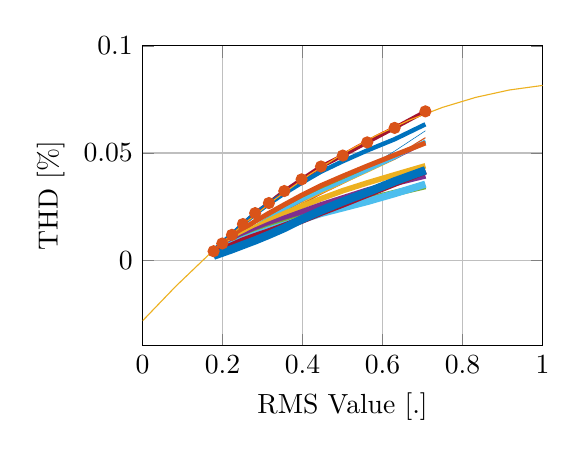
\begin{tikzpicture}

\begin{axis}[%
width=2.0in,
height=1.5in,
at={(0.758in,0.481in)},
scale only axis,
xmin=0,
xmax=1,
xlabel={RMS Value [.]},
xmajorgrids,
ymin=-0.04,
ymax=0.1,
ylabel={THD [\%]},
y tick label style={/pgf/number format/fixed},
ymajorgrids,
axis background/.style={fill=white},
legend style={legend cell align=left,align=left,draw=white!15!black},
every axis legend/.code={\let\addlegendentry\relax}
]
\addplot [color=mycolor1,solid,line width=0.2pt]
  table[row sep=crcr]{%
0.177615489572042	0.00281550869189747\\
0.19928785706971	0.00579102233850549\\
0.223604653350506	0.00833724920963191\\
0.250888547527061	0.011089449640169\\
0.281501580298378	0.0140535489887201\\
0.315849968009946	0.0168712055985728\\
0.354389492897844	0.020978580147255\\
0.397631551042096	0.0256346127296753\\
0.446149938281945	0.0309903755999393\\
0.500588464138024	0.0366268475572401\\
0.561669494773539	0.0431598178212298\\
0.630203538354371	0.0508665295530352\\
0.7071	0.060327374914144\\
};
\addlegendentry{150 Hz};

\addplot [color=mycolor2,solid,line width=0.4pt]
  table[row sep=crcr]{%
0.177615489572042	0.00288242857291702\\
0.19928785706971	0.00601942003919589\\
0.223604653350506	0.00838737458944496\\
0.250888547527061	0.011073810857975\\
0.281501580298378	0.0141679628103181\\
0.315849968009946	0.0178221035144654\\
0.354389492897844	0.0216784462385848\\
0.397631551042096	0.026223745606834\\
0.446149938281945	0.0308388124324108\\
0.500588464138024	0.0357813457369064\\
0.561669494773539	0.041536895541812\\
0.630203538354371	0.0482152631044592\\
0.7071	0.0571206231147102\\
};
\addlegendentry{160 Hz};

\addplot [color=mycolor3,solid,line width=0.6pt]
  table[row sep=crcr]{%
0.177615489572042	0.00261738928498524\\
0.19928785706971	0.00538808113967551\\
0.223604653350506	0.0078163563430788\\
0.250888547527061	0.0110860314848712\\
0.281501580298378	0.0146542555662576\\
0.315849968009946	0.0186356922477342\\
0.354389492897844	0.0229297722180043\\
0.397631551042096	0.0270974616675691\\
0.446149938281945	0.0312365142100714\\
0.500588464138024	0.0359522578433619\\
0.561669494773539	0.0411599229427607\\
0.630203538354371	0.047158317467538\\
0.7071	0.0552352483180093\\
};
\addlegendentry{170 Hz};

\addplot [color=mycolor4,solid,line width=0.8pt]
  table[row sep=crcr]{%
0.177615489572042	0.00264182868343871\\
0.19928785706971	0.00587295661862796\\
0.223604653350506	0.00853663083626045\\
0.250888547527061	0.0118405248558538\\
0.281501580298378	0.0156254204927327\\
0.315849968009946	0.0192963319906929\\
0.354389492897844	0.0232121167082912\\
0.397631551042096	0.0277137334965289\\
0.446149938281945	0.0326356988993767\\
0.500588464138024	0.0369400135275638\\
0.561669494773539	0.0420953038506985\\
0.630203538354371	0.0474638752528505\\
0.7071	0.0545561914975807\\
};
\addlegendentry{180 Hz};

\addplot [color=mycolor5,solid,line width=1.0pt]
  table[row sep=crcr]{%
0.177615489572042	0.0032918632385986\\
0.19928785706971	0.00633463551470011\\
0.223604653350506	0.00884255159807594\\
0.250888547527061	0.0117739998790346\\
0.281501580298378	0.0156041715418844\\
0.315849968009946	0.0198208562789661\\
0.354389492897844	0.024243868188967\\
0.397631551042096	0.029006101103932\\
0.446149938281945	0.0337966681496026\\
0.500588464138024	0.0382490473564407\\
0.561669494773539	0.0431126808921298\\
0.630203538354371	0.0485831957181763\\
0.7071	0.0552774021794615\\
};
\addlegendentry{190 Hz};

\addplot [color=mycolor6,solid,line width=1.2pt]
  table[row sep=crcr]{%
0.177615489572042	0.00317103913305149\\
0.19928785706971	0.00578459442385685\\
0.223604653350506	0.00859240572572188\\
0.250888547527061	0.01201336799769\\
0.281501580298378	0.0155826860285665\\
0.315849968009946	0.0194348765928136\\
0.354389492897844	0.0237139003688241\\
0.397631551042096	0.0279944680420928\\
0.446149938281945	0.0323075337872231\\
0.500588464138024	0.0366707202218788\\
0.561669494773539	0.0418715222262427\\
0.630203538354371	0.0478062397409383\\
0.7071	0.0556067507707686\\
};
\addlegendentry{200 Hz};

\addplot [color=mycolor7,solid,line width=1.4pt]
  table[row sep=crcr]{%
0.177615489572042	0.00413423080837976\\
0.19928785706971	0.00774964057906419\\
0.223604653350506	0.0117955883224023\\
0.250888547527061	0.0168115285473131\\
0.281501580298378	0.0219299032271524\\
0.315849968009946	0.0266197966761756\\
0.354389492897844	0.0322288609486394\\
0.397631551042096	0.0376699883114906\\
0.446149938281945	0.0436875465590951\\
0.500588464138024	0.0487868389585705\\
0.561669494773539	0.0549257978429372\\
0.630203538354371	0.0616939335010604\\
0.7071	0.0694140313161441\\
};
\addlegendentry{210 Hz};

\addplot [color=mycolor1,solid,line width=1.6pt]
  table[row sep=crcr]{%
0.177615489572042	0.00423380770292324\\
0.19928785706971	0.00829210334354166\\
0.223604653350506	0.0119557086298509\\
0.250888547527061	0.0168455576619543\\
0.281501580298378	0.021612723677298\\
0.315849968009946	0.0262875525282313\\
0.354389492897844	0.031099636915235\\
0.397631551042096	0.0360419174635684\\
0.446149938281945	0.0412680215486007\\
0.500588464138024	0.0461215304761316\\
0.561669494773539	0.0511786507340304\\
0.630203538354371	0.0564006977938137\\
0.7071	0.0633747350783306\\
};
\addlegendentry{220 Hz};

\addplot [color=mycolor2,solid,line width=1.8pt]
  table[row sep=crcr]{%
0.177615489572042	0.00400754081472606\\
0.19928785706971	0.00713064401586951\\
0.223604653350506	0.0103907811238824\\
0.250888547527061	0.0143313956887522\\
0.281501580298378	0.018106014953588\\
0.315849968009946	0.0218473369346513\\
0.354389492897844	0.025853310510801\\
0.397631551042096	0.0302516700934496\\
0.446149938281945	0.0347647356260932\\
0.500588464138024	0.0391704710956094\\
0.561669494773539	0.0439055678661902\\
0.630203538354371	0.0490180836456588\\
0.7071	0.054639966799512\\
};
\addlegendentry{230 Hz};

\addplot [color=mycolor3,solid,line width=2.0pt]
  table[row sep=crcr]{%
0.177615489572042	0.00367380070843936\\
0.19928785706971	0.00589162307251598\\
0.223604653350506	0.00883590838205179\\
0.250888547527061	0.0120429236956981\\
0.281501580298378	0.0150883172278887\\
0.315849968009946	0.0183802964754995\\
0.354389492897844	0.0217154649953816\\
0.397631551042096	0.0251346906716686\\
0.446149938281945	0.0286448816379722\\
0.500588464138024	0.0323797134157115\\
0.561669494773539	0.0360263600414313\\
0.630203538354371	0.0398232399559189\\
0.7071	0.0440112464576971\\
};
\addlegendentry{240 Hz};

\addplot [color=mycolor4,solid,line width=2.2pt]
  table[row sep=crcr]{%
0.177615489572042	0.00315080086872717\\
0.19928785706971	0.0052972335419083\\
0.223604653350506	0.00803632000398619\\
0.250888547527061	0.0108280950147934\\
0.281501580298378	0.0137537283675673\\
0.315849968009946	0.0165165376838169\\
0.354389492897844	0.0193882382631167\\
0.397631551042096	0.022350336916317\\
0.446149938281945	0.0256319915139642\\
0.500588464138024	0.0288840084404326\\
0.561669494773539	0.0325254204164891\\
0.630203538354371	0.0359080789226022\\
0.7071	0.0394232757762628\\
};
\addlegendentry{250 Hz};

\addplot [color=mycolor5,solid,line width=2.4pt]
  table[row sep=crcr]{%
0.177615489572042	0.00258507571556675\\
0.19928785706971	0.00486020858039155\\
0.223604653350506	0.00722373245727585\\
0.250888547527061	0.00972492589959707\\
0.281501580298378	0.0122181417088705\\
0.315849968009946	0.0147044314296091\\
0.354389492897844	0.0171247683958299\\
0.397631551042096	0.019545293096281\\
0.446149938281945	0.0223503705529437\\
0.500588464138024	0.0250359641244579\\
0.561669494773539	0.028071112410699\\
0.630203538354371	0.031282722335403\\
0.7071	0.0346057314578435\\
};
\addlegendentry{260 Hz};

\addplot [color=mycolor6,solid,line width=2.6pt]
  table[row sep=crcr]{%
0.177615489572042	0.00251780718381692\\
0.19928785706971	0.00485820999937342\\
0.223604653350506	0.00718112278971849\\
0.250888547527061	0.00950032403924523\\
0.281501580298378	0.0117544824167738\\
0.315849968009946	0.014011548029271\\
0.354389492897844	0.0163182785123765\\
0.397631551042096	0.0188514284663503\\
0.446149938281945	0.021762459584876\\
0.500588464138024	0.0243748394402199\\
0.561669494773539	0.0273322541586317\\
0.630203538354371	0.0310096933636042\\
0.7071	0.0354348526250838\\
};
\addlegendentry{270 Hz};

\addplot [color=mycolor7,solid,line width=2.8pt]
  table[row sep=crcr]{%
0.177615489572042	0.00245430802132249\\
0.19928785706971	0.0045375132996648\\
0.223604653350506	0.00655742377411303\\
0.250888547527061	0.00878266514929233\\
0.281501580298378	0.0108702175770487\\
0.315849968009946	0.0130585010307198\\
0.354389492897844	0.0156826456731349\\
0.397631551042096	0.018729115295188\\
0.446149938281945	0.0224446540379895\\
0.500588464138024	0.0262959976010849\\
0.561669494773539	0.0308897133816619\\
0.630203538354371	0.0359935387977394\\
0.7071	0.0417717415197022\\
};
\addlegendentry{280 Hz};

\addplot [color=mycolor1,solid,line width=3.0pt,forget plot]
  table[row sep=crcr]{%
0.177615489572042	0.00205368263706797\\
0.19928785706971	0.00348379415594429\\
0.223604653350506	0.00508702990168937\\
0.250888547527061	0.00703635792364254\\
0.281501580298378	0.00919490750505369\\
0.315849968009946	0.0118280776578328\\
0.354389492897844	0.0149702620002119\\
0.397631551042096	0.0190105008575072\\
0.446149938281945	0.0231148796883891\\
0.500588464138024	0.0273213516432495\\
0.561669494773539	0.0316348501218829\\
0.630203538354371	0.0367512134931775\\
0.7071	0.0419360163557166\\
};
\addplot [color=mycolor2,only marks,mark=*,mark options={solid}]
  table[row sep=crcr]{%
0.177615489572042	0.00413423080837976\\
0.19928785706971	0.00774964057906419\\
0.223604653350506	0.0117955883224023\\
0.250888547527061	0.0168115285473131\\
0.281501580298378	0.0219299032271524\\
0.315849968009946	0.0266197966761756\\
0.354389492897844	0.0322288609486394\\
0.397631551042096	0.0376699883114906\\
0.446149938281945	0.0436875465590951\\
0.500588464138024	0.0487868389585705\\
0.561669494773539	0.0549257978429372\\
0.630203538354371	0.0616939335010604\\
0.7071	0.0694140313161441\\
};
\addlegendentry{data};

\addplot [color=red,solid]
  table[row sep=crcr]{%
0.177615489572042	0.00459173856686059\\
0.17814497408247	0.00468124071101805\\
0.178674458592898	0.00477069135324276\\
0.179203943103326	0.00486009049353471\\
0.179733427613754	0.00494943813189391\\
0.180262912124182	0.00503873426832036\\
0.18079239663461	0.00512797890281404\\
0.181321881145038	0.00521717203537498\\
0.181851365655466	0.00530631366600316\\
0.182380850165894	0.00539540379469858\\
0.182910334676322	0.00548444242146126\\
0.18343981918675	0.00557342954629118\\
0.183969303697178	0.00566236516918835\\
0.184498788207606	0.00575124929015276\\
0.185028272718034	0.00584008190918441\\
0.185557757228462	0.00592886302628332\\
0.18608724173889	0.00601759264144946\\
0.186616726249318	0.00610627075468285\\
0.187146210759746	0.00619489736598349\\
0.187675695270174	0.00628347247535138\\
0.188205179780602	0.00637199608278652\\
0.18873466429103	0.0064604681882889\\
0.189264148801457	0.00654888879185852\\
0.189793633311885	0.00663725789349538\\
0.190323117822313	0.0067255754931995\\
0.190852602332741	0.00681384159097086\\
0.191382086843169	0.00690205618680947\\
0.191911571353597	0.00699021928071532\\
0.192441055864025	0.00707833087268842\\
0.192970540374453	0.00716639096272876\\
0.193500024884881	0.00725439955083636\\
0.194029509395309	0.00734235663701119\\
0.194558993905737	0.00743026222125327\\
0.195088478416165	0.0075181163035626\\
0.195617962926593	0.00760591888393918\\
0.196147447437021	0.007693669962383\\
0.196676931947449	0.00778136953889406\\
0.197206416457877	0.00786901761347238\\
0.197735900968305	0.00795661418611793\\
0.198265385478733	0.00804415925683073\\
0.198794869989161	0.00813165282561078\\
0.19928785706971	0.00821306915312126\\
0.199324354499589	0.00821909489245808\\
0.199853839010017	0.00830648545737261\\
0.200383323520445	0.00839382452035441\\
0.200912808030873	0.00848111208140344\\
0.201442292541301	0.00856834814051972\\
0.201971777051728	0.00865553269770324\\
0.202501261562156	0.00874266575295401\\
0.203030746072584	0.00882974730627203\\
0.203560230583012	0.00891677735765729\\
0.20408971509344	0.0090037559071098\\
0.204619199603868	0.00909068295462955\\
0.205148684114296	0.00917755850021655\\
0.205678168624724	0.0092643825438708\\
0.206207653135152	0.00935115508559229\\
0.20673713764558	0.00943787612538102\\
0.207266622156008	0.00952454566323701\\
0.207796106666436	0.00961116369916024\\
0.208325591176864	0.00969773023315072\\
0.208855075687292	0.00978424526520844\\
0.20938456019772	0.0098707087953334\\
0.209914044708148	0.00995712082352562\\
0.210443529218576	0.0100434813497851\\
0.210973013729004	0.0101297903741118\\
0.211502498239432	0.0102160478965057\\
0.21203198274986	0.0103022539169669\\
0.212561467260288	0.0103884084354954\\
0.213090951770716	0.0104745114520911\\
0.213620436281144	0.010560562966754\\
0.214149920791571	0.0106465629794842\\
0.214679405301999	0.0107325114902816\\
0.215208889812427	0.0108184084991463\\
0.215738374322855	0.0109042540060782\\
0.216267858833283	0.0109900480110773\\
0.216797343343711	0.0110757905141438\\
0.217326827854139	0.0111614815152774\\
0.217856312364567	0.0112471210144783\\
0.218385796874995	0.0113327090117465\\
0.218915281385423	0.0114182455070818\\
0.219444765895851	0.0115037305004845\\
0.219974250406279	0.0115891639919544\\
0.220503734916707	0.0116745459814915\\
0.221033219427135	0.0117598764690959\\
0.221562703937563	0.0118451554547675\\
0.222092188447991	0.0119303829385064\\
0.222621672958419	0.0120155589203125\\
0.223151157468847	0.0121006834001858\\
0.223604653350506	0.0121735503497022\\
0.223680641979275	0.0121857563781264\\
0.224210126489703	0.0122707778541343\\
0.224739611000131	0.0123557478282094\\
0.225269095510559	0.0124406663003517\\
0.225798580020987	0.0125255332705613\\
0.226328064531414	0.0126103487388382\\
0.226857549041842	0.0126951127051822\\
0.22738703355227	0.0127798251695936\\
0.227916518062698	0.0128644861320721\\
0.228446002573126	0.0129490955926179\\
0.228975487083554	0.013033653551231\\
0.229504971593982	0.0131181600079113\\
0.23003445610441	0.0132026149626589\\
0.230563940614838	0.0132870184154737\\
0.231093425125266	0.0133713703663557\\
0.231622909635694	0.013455670815305\\
0.232152394146122	0.0135399197623216\\
0.23268187865655	0.0136241172074054\\
0.233211363166978	0.0137082631505564\\
0.233740847677406	0.0137923575917747\\
0.234270332187834	0.0138764005310602\\
0.234799816698262	0.013960391968413\\
0.23532930120869	0.014044331903833\\
0.235858785719118	0.0141282203373202\\
0.236388270229546	0.0142120572688747\\
0.236917754739974	0.0142958426984965\\
0.237447239250402	0.0143795766261855\\
0.23797672376083	0.0144632590519417\\
0.238506208271258	0.0145468899757652\\
0.239035692781685	0.014630469397656\\
0.239565177292113	0.0147139973176139\\
0.240094661802541	0.0147974737356392\\
0.240624146312969	0.0148808986517316\\
0.241153630823397	0.0149642720658914\\
0.241683115333825	0.0150475939781183\\
0.242212599844253	0.0151308643884125\\
0.242742084354681	0.015214083296774\\
0.243271568865109	0.0152972507032027\\
0.243801053375537	0.0153803666076986\\
0.244330537885965	0.0154634310102618\\
0.244860022396393	0.0155464439108923\\
0.245389506906821	0.01562940530959\\
0.245918991417249	0.0157123152063549\\
0.246448475927677	0.0157951736011871\\
0.246977960438105	0.0158779804940865\\
0.247507444948533	0.0159607358850532\\
0.248036929458961	0.0160434397740871\\
0.248566413969389	0.0161260921611882\\
0.249095898479817	0.0162086930463567\\
0.249625382990245	0.0162912424295923\\
0.250154867500673	0.0163737403108952\\
0.250684352011101	0.0164561866902653\\
0.250888547527061	0.0164879683469069\\
0.251213836521529	0.0165385815677027\\
0.251743321031956	0.0166209249432074\\
0.252272805542384	0.0167032168167793\\
0.252802290052812	0.0167854571884184\\
0.25333177456324	0.0168676460581248\\
0.253861259073668	0.0169497834258984\\
0.254390743584096	0.0170318692917392\\
0.254920228094524	0.0171139036556474\\
0.255449712604952	0.0171958865176227\\
0.25597919711538	0.0172778178776653\\
0.256508681625808	0.0173596977357752\\
0.257038166136236	0.0174415260919523\\
0.257567650646664	0.0175233029461966\\
0.258097135157092	0.0176050282985082\\
0.25862661966752	0.017686702148887\\
0.259156104177948	0.0177683244973331\\
0.259685588688376	0.0178498953438464\\
0.260215073198804	0.017931414688427\\
0.260744557709232	0.0180128825310748\\
0.26127404221966	0.0180942988717899\\
0.261803526730088	0.0181756637105722\\
0.262333011240516	0.0182569770474217\\
0.262862495750944	0.0183382388823385\\
0.263391980261372	0.0184194492153226\\
0.263921464771799	0.0185006080463739\\
0.264450949282227	0.0185817153754924\\
0.264980433792655	0.0186627712026782\\
0.265509918303083	0.0187437755279312\\
0.266039402813511	0.0188247283512515\\
0.266568887323939	0.018905629672639\\
0.267098371834367	0.0189864794920938\\
0.267627856344795	0.0190672778096158\\
0.268157340855223	0.0191480246252051\\
0.268686825365651	0.0192287199388616\\
0.269216309876079	0.0193093637505853\\
0.269745794386507	0.0193899560603763\\
0.270275278896935	0.0194704968682346\\
0.270804763407363	0.01955098617416\\
0.271334247917791	0.0196314239781528\\
0.271863732428219	0.0197118102802128\\
0.272393216938647	0.01979214508034\\
0.272922701449075	0.0198724283785345\\
0.273452185959503	0.0199526601747962\\
0.273981670469931	0.0200328404691251\\
0.274511154980359	0.0201129692615213\\
0.275040639490787	0.0201930465519848\\
0.275570124001215	0.0202730723405155\\
0.276099608511643	0.0203530466271134\\
0.27662909302207	0.0204329694117786\\
0.277158577532498	0.0205128406945111\\
0.277688062042926	0.0205926604753108\\
0.278217546553354	0.0206724287541777\\
0.278747031063782	0.0207521455311119\\
0.27927651557421	0.0208318108061133\\
0.279806000084638	0.020911424579182\\
0.280335484595066	0.0209909868503179\\
0.280864969105494	0.021070497619521\\
0.281394453615922	0.0211499568867914\\
0.281501580298378	0.0211660270281829\\
0.28192393812635	0.0212293646521291\\
0.282453422636778	0.021308720915534\\
0.282982907147206	0.0213880256770061\\
0.283512391657634	0.0214672789365455\\
0.284041876168062	0.0215464806941522\\
0.28457136067849	0.021625630949826\\
0.285100845188918	0.0217047297035672\\
0.285630329699346	0.0217837769553755\\
0.286159814209774	0.0218627727052511\\
0.286689298720202	0.021941716953194\\
0.28721878323063	0.0220206096992041\\
0.287748267741058	0.0220994509432815\\
0.288277752251486	0.0221782406854261\\
0.288807236761913	0.0222569789256379\\
0.289336721272341	0.022335665663917\\
0.289866205782769	0.0224143009002634\\
0.290395690293197	0.0224928846346769\\
0.290925174803625	0.0225714168671578\\
0.291454659314053	0.0226498975977059\\
0.291984143824481	0.0227283268263212\\
0.292513628334909	0.0228067045530038\\
0.293043112845337	0.0228850307777536\\
0.293572597355765	0.0229633055005706\\
0.294102081866193	0.0230415287214549\\
0.294631566376621	0.0231197004404065\\
0.295161050887049	0.0231978206574253\\
0.295690535397477	0.0232758893725113\\
0.296220019907905	0.0233539065856646\\
0.296749504418333	0.0234318722968852\\
0.297278988928761	0.0235097865061729\\
0.297808473439189	0.023587649213528\\
0.298337957949617	0.0236654604189502\\
0.298867442460045	0.0237432201224398\\
0.299396926970473	0.0238209283239965\\
0.299926411480901	0.0238985850236205\\
0.300455895991329	0.0239761902213118\\
0.300985380501756	0.0240537439170703\\
0.301514865012184	0.024131246110896\\
0.302044349522612	0.024208696802789\\
0.30257383403304	0.0242860959927493\\
0.303103318543468	0.0243634436807768\\
0.303632803053896	0.0244407398668715\\
0.304162287564324	0.0245179845510335\\
0.304691772074752	0.0245951777332627\\
0.30522125658518	0.0246723194135592\\
0.305750741095608	0.0247494095919229\\
0.306280225606036	0.0248264482683538\\
0.306809710116464	0.024903435442852\\
0.307339194626892	0.0249803711154175\\
0.30786867913732	0.0250572552860502\\
0.308398163647748	0.0251340879547501\\
0.308927648158176	0.0252108691215173\\
0.309457132668604	0.0252875987863518\\
0.309986617179032	0.0253642769492535\\
0.31051610168946	0.0254409036102224\\
0.311045586199888	0.0255174787692586\\
0.311575070710316	0.025594002426362\\
0.312104555220744	0.0256704745815326\\
0.312634039731172	0.0257468952347706\\
0.3131635242416	0.0258232643860757\\
0.313693008752027	0.0258995820354481\\
0.314222493262455	0.0259758481828878\\
0.314751977772883	0.0260520628283947\\
0.315281462283311	0.0261282259719688\\
0.315810946793739	0.0262043376136102\\
0.315849968009946	0.0262099447463572\\
0.316340431304167	0.0262803977533188\\
0.316869915814595	0.0263564063910947\\
0.317399400325023	0.0264323635269378\\
0.317928884835451	0.0265082691608482\\
0.318458369345879	0.0265841232928258\\
0.318987853856307	0.0266599259228707\\
0.319517338366735	0.0267356770509828\\
0.320046822877163	0.0268113766771622\\
0.320576307387591	0.0268870248014087\\
0.321105791898019	0.0269626214237226\\
0.321635276408447	0.0270381665441037\\
0.322164760918875	0.027113660162552\\
0.322694245429303	0.0271891022790676\\
0.323223729939731	0.0272644928936504\\
0.323753214450159	0.0273398320063005\\
0.324282698960587	0.0274151196170178\\
0.324812183471015	0.0274903557258024\\
0.325341667981443	0.0275655403326542\\
0.32587115249187	0.0276406734375733\\
0.326400637002298	0.0277157550405596\\
0.326930121512726	0.0277907851416131\\
0.327459606023154	0.0278657637407339\\
0.327989090533582	0.027940690837922\\
0.32851857504401	0.0280155664331773\\
0.329048059554438	0.0280903905264998\\
0.329577544064866	0.0281651631178896\\
0.330107028575294	0.0282398842073466\\
0.330636513085722	0.0283145537948709\\
0.33116599759615	0.0283891718804624\\
0.331695482106578	0.0284637384641212\\
0.332224966617006	0.0285382535458471\\
0.332754451127434	0.0286127171256404\\
0.333283935637862	0.0286871292035009\\
0.33381342014829	0.0287614897794287\\
0.334342904658718	0.0288357988534237\\
0.334872389169146	0.0289100564254859\\
0.335401873679574	0.0289842624956154\\
0.335931358190002	0.0290584170638121\\
0.33646084270043	0.0291325201300761\\
0.336990327210858	0.0292065716944073\\
0.337519811721286	0.0292805717568058\\
0.338049296231714	0.0293545203172715\\
0.338578780742141	0.0294284173758044\\
0.339108265252569	0.0295022629324047\\
0.339637749762997	0.0295760569870721\\
0.340167234273425	0.0296497995398068\\
0.340696718783853	0.0297234905906087\\
0.341226203294281	0.0297971301394779\\
0.341755687804709	0.0298707181864144\\
0.342285172315137	0.029944254731418\\
0.342814656825565	0.030017739774489\\
0.343344141335993	0.0300911733156272\\
0.343873625846421	0.0301645553548326\\
0.344403110356849	0.0302378858921052\\
0.344932594867277	0.0303111649274451\\
0.345462079377705	0.0303843924608523\\
0.345991563888133	0.0304575684923267\\
0.346521048398561	0.0305306930218684\\
0.347050532908989	0.0306037660494772\\
0.347580017419417	0.0306767875751534\\
0.348109501929845	0.0307497575988968\\
0.348638986440273	0.0308226761207074\\
0.349168470950701	0.0308955431405853\\
0.349697955461129	0.0309683586585304\\
0.350227439971557	0.0310411226745428\\
0.350756924481984	0.0311138351886224\\
0.351286408992412	0.0311864962007693\\
0.35181589350284	0.0312591057109834\\
0.352345378013268	0.0313316637192647\\
0.352874862523696	0.0314041702256133\\
0.353404347034124	0.0314766252300292\\
0.353933831544552	0.0315490287325122\\
0.354389492897844	0.031611296175287\\
0.35446331605498	0.0316213807330626\\
0.354992800565408	0.0316936812316802\\
0.355522285075836	0.031765930228365\\
0.356051769586264	0.0318381277231171\\
0.356581254096692	0.0319102737159364\\
0.35711073860712	0.0319823682068229\\
0.357640223117548	0.0320544111957768\\
0.358169707627976	0.0321264026827978\\
0.358699192138404	0.0321983426678861\\
0.359228676648832	0.0322702311510417\\
0.35975816115926	0.0323420681322645\\
0.360287645669688	0.0324138536115545\\
0.360817130180116	0.0324855875889118\\
0.361346614690544	0.0325572700643363\\
0.361876099200972	0.0326289010378281\\
0.3624055837114	0.0327004805093871\\
0.362935068221828	0.0327720084790134\\
0.363464552732255	0.0328434849467069\\
0.363994037242683	0.0329149099124677\\
0.364523521753111	0.0329862833762957\\
0.365053006263539	0.0330576053381909\\
0.365582490773967	0.0331288757981534\\
0.366111975284395	0.0332000947561832\\
0.366641459794823	0.0332712622122802\\
0.367170944305251	0.0333423781664444\\
0.367700428815679	0.0334134426186759\\
0.368229913326107	0.0334844555689746\\
0.368759397836535	0.0335554170173406\\
0.369288882346963	0.0336263269637738\\
0.369818366857391	0.0336971854082743\\
0.370347851367819	0.033767992350842\\
0.370877335878247	0.033838747791477\\
0.371406820388675	0.0339094517301791\\
0.371936304899103	0.0339801041669486\\
0.372465789409531	0.0340507051017853\\
0.372995273919959	0.0341212545346892\\
0.373524758430387	0.0341917524656604\\
0.374054242940815	0.0342621988946989\\
0.374583727451243	0.0343325938218045\\
0.375113211961671	0.0344029372469775\\
0.375642696472098	0.0344732291702176\\
0.376172180982526	0.0345434695915251\\
0.376701665492954	0.0346136585108997\\
0.377231150003382	0.0346837959283416\\
0.37776063451381	0.0347538818438508\\
0.378290119024238	0.0348239162574272\\
0.378819603534666	0.0348938991690708\\
0.379349088045094	0.0349638305787817\\
0.379878572555522	0.0350337104865599\\
0.38040805706595	0.0351035388924052\\
0.380937541576378	0.0351733157963179\\
0.381467026086806	0.0352430411982977\\
0.381996510597234	0.0353127150983449\\
0.382525995107662	0.0353823374964592\\
0.38305547961809	0.0354519083926408\\
0.383584964128518	0.0355214277868897\\
0.384114448638946	0.0355908956792058\\
0.384643933149374	0.0356603120695892\\
0.385173417659802	0.0357296769580398\\
0.38570290217023	0.0357989903445576\\
0.386232386680658	0.0358682522291427\\
0.386761871191086	0.035937462611795\\
0.387291355701514	0.0360066214925146\\
0.387820840211942	0.0360757288713014\\
0.388350324722369	0.0361447847481555\\
0.388879809232797	0.0362137891230768\\
0.389409293743225	0.0362827419960654\\
0.389938778253653	0.0363516433671212\\
0.390468262764081	0.0364204932362443\\
0.390997747274509	0.0364892916034346\\
0.391527231784937	0.0365580384686921\\
0.392056716295365	0.0366267338320169\\
0.392586200805793	0.0366953776934089\\
0.393115685316221	0.0367639700528682\\
0.393645169826649	0.0368325109103948\\
0.394174654337077	0.0369010002659885\\
0.394704138847505	0.0369694381196495\\
0.395233623357933	0.0370378244713778\\
0.395763107868361	0.0371061593211733\\
0.396292592378789	0.0371744426690361\\
0.396822076889217	0.0372426745149661\\
0.397351561399645	0.0373108548589633\\
0.397631551042096	0.0373468875797179\\
0.397881045910073	0.0373789837010278\\
0.398410530420501	0.0374470610411596\\
0.398940014930929	0.0375150868793586\\
0.399469499441357	0.0375830612156248\\
0.399998983951785	0.0376509840499583\\
0.400528468462212	0.037718855382359\\
0.40105795297264	0.037786675212827\\
0.401587437483068	0.0378544435413622\\
0.402116921993496	0.0379221603679647\\
0.402646406503924	0.0379898256926344\\
0.403175891014352	0.0380574395153713\\
0.40370537552478	0.0381250018361755\\
0.404234860035208	0.038192512655047\\
0.404764344545636	0.0382599719719857\\
0.405293829056064	0.0383273797869916\\
0.405823313566492	0.0383947361000648\\
0.40635279807692	0.0384620409112053\\
0.406882282587348	0.0385292942204129\\
0.407411767097776	0.0385964960276878\\
0.407941251608204	0.03866364633303\\
0.408470736118632	0.0387307451364394\\
0.40900022062906	0.0387977924379161\\
0.409529705139488	0.03886478823746\\
0.410059189649916	0.0389317325350712\\
0.410588674160344	0.0389986253307496\\
0.411118158670772	0.0390654666244952\\
0.4116476431812	0.0391322564163081\\
0.412177127691628	0.0391989947061882\\
0.412706612202056	0.0392656814941356\\
0.413236096712484	0.0393323167801502\\
0.413765581222911	0.0393989005642321\\
0.414295065733339	0.0394654328463812\\
0.414824550243767	0.0395319136265976\\
0.415354034754195	0.0395983429048812\\
0.415883519264623	0.0396647206812321\\
0.416413003775051	0.0397310469556502\\
0.416942488285479	0.0397973217281355\\
0.417471972795907	0.0398635449986881\\
0.418001457306335	0.039929716767308\\
0.418530941816763	0.039995837033995\\
0.419060426327191	0.0400619057987494\\
0.419589910837619	0.040127923061571\\
0.420119395348047	0.0401938888224598\\
0.420648879858475	0.0402598030814159\\
0.421178364368903	0.0403256658384392\\
0.421707848879331	0.0403914770935297\\
0.422237333389759	0.0404572368466875\\
0.422766817900187	0.0405229450979126\\
0.423296302410615	0.0405886018472049\\
0.423825786921043	0.0406542070945644\\
0.424355271431471	0.0407197608399912\\
0.424884755941899	0.0407852630834853\\
0.425414240452327	0.0408507138250465\\
0.425943724962754	0.0409161130646751\\
0.426473209473182	0.0409814608023708\\
0.42700269398361	0.0410467570381339\\
0.427532178494038	0.0411120017719641\\
0.428061663004466	0.0411771950038616\\
0.428591147514894	0.0412423367338264\\
0.429120632025322	0.0413074269618584\\
0.42965011653575	0.0413724656879577\\
0.430179601046178	0.0414374529121241\\
0.430709085556606	0.0415023886343579\\
0.431238570067034	0.0415672728546589\\
0.431768054577462	0.0416321055730271\\
0.43229753908789	0.0416968867894626\\
0.432827023598318	0.0417616165039653\\
0.433356508108746	0.0418262947165353\\
0.433885992619174	0.0418909214271725\\
0.434415477129602	0.041955496635877\\
0.43494496164003	0.0420200203426487\\
0.435474446150458	0.0420844925474876\\
0.436003930660886	0.0421489132503938\\
0.436533415171314	0.0422132824513673\\
0.437062899681742	0.042277600150408\\
0.43759238419217	0.0423418663475159\\
0.438121868702598	0.0424060810426911\\
0.438651353213025	0.0424702442359335\\
0.439180837723453	0.0425343559272432\\
0.439710322233881	0.0425984161166201\\
0.440239806744309	0.0426624248040643\\
0.440769291254737	0.0427263819895757\\
0.441298775765165	0.0427902876731544\\
0.441828260275593	0.0428541418548003\\
0.442357744786021	0.0429179445345134\\
0.442887229296449	0.0429816957122938\\
0.443416713806877	0.0430453953881415\\
0.443946198317305	0.0431090435620564\\
0.444475682827733	0.0431726402340385\\
0.445005167338161	0.0432361854040879\\
0.445534651848589	0.0432996790722045\\
0.446064136359017	0.0433631212383884\\
0.446149938281945	0.0433733970674663\\
0.446593620869445	0.0434265119026395\\
0.447123105379873	0.0434898510649578\\
0.447652589890301	0.0435531387253435\\
0.448182074400729	0.0436163748837963\\
0.448711558911157	0.0436795595403164\\
0.449241043421585	0.0437426926949038\\
0.449770527932013	0.0438057743475584\\
0.450300012442441	0.0438688044982802\\
0.450829496952868	0.0439317831470693\\
0.451358981463296	0.0439947102939256\\
0.451888465973724	0.0440575859388492\\
0.452417950484152	0.04412041008184\\
0.45294743499458	0.0441831827228981\\
0.453476919505008	0.0442459038620234\\
0.454006404015436	0.044308573499216\\
0.454535888525864	0.0443711916344758\\
0.455065373036292	0.0444337582678028\\
0.45559485754672	0.0444962733991971\\
0.456124342057148	0.0445587370286587\\
0.456653826567576	0.0446211491561874\\
0.457183311078004	0.0446835097817835\\
0.457712795588432	0.0447458189054468\\
0.45824228009886	0.0448080765271773\\
0.458771764609288	0.0448702826469751\\
0.459301249119716	0.0449324372648401\\
0.459830733630144	0.0449945403807724\\
0.460360218140572	0.0450565919947719\\
0.460889702651	0.0451185921068386\\
0.461419187161428	0.0451805407169726\\
0.461948671671856	0.0452424378251739\\
0.462478156182284	0.0453042834314423\\
0.463007640692712	0.0453660775357781\\
0.463537125203139	0.0454278201381811\\
0.464066609713567	0.0454895112386513\\
0.464596094223995	0.0455511508371888\\
0.465125578734423	0.0456127389337935\\
0.465655063244851	0.0456742755284655\\
0.466184547755279	0.0457357606212047\\
0.466714032265707	0.0457971942120112\\
0.467243516776135	0.0458585763008849\\
0.467773001286563	0.0459199068878258\\
0.468302485796991	0.045981185972834\\
0.468831970307419	0.0460424135559095\\
0.469361454817847	0.0461035896370522\\
0.469890939328275	0.0461647142162621\\
0.470420423838703	0.0462257872935393\\
0.470949908349131	0.0462868088688837\\
0.471479392859559	0.0463477789422954\\
0.472008877369987	0.0464086975137743\\
0.472538361880415	0.0464695645833205\\
0.473067846390843	0.0465303801509339\\
0.473597330901271	0.0465911442166145\\
0.474126815411699	0.0466518567803624\\
0.474656299922127	0.0467125178421776\\
0.475185784432555	0.04677312740206\\
0.475715268942982	0.0468336854600096\\
0.47624475345341	0.0468941920160265\\
0.476774237963838	0.0469546470701106\\
0.477303722474266	0.047015050622262\\
0.477833206984694	0.0470754026724807\\
0.478362691495122	0.0471357032207665\\
0.47889217600555	0.0471959522671196\\
0.479421660515978	0.04725614981154\\
0.479951145026406	0.0473162958540276\\
0.480480629536834	0.0473763903945825\\
0.481010114047262	0.0474364334332046\\
0.48153959855769	0.0474964249698939\\
0.482069083068118	0.0475563650046505\\
0.482598567578546	0.0476162535374743\\
0.483128052088974	0.0476760905683654\\
0.483657536599402	0.0477358760973237\\
0.48418702110983	0.0477956101243493\\
0.484716505620258	0.0478552926494421\\
0.485245990130686	0.0479149236726022\\
0.485775474641114	0.0479745031938295\\
0.486304959151542	0.0480340312131241\\
0.48683444366197	0.0480935077304859\\
0.487363928172397	0.0481529327459149\\
0.487893412682825	0.0482123062594112\\
0.488422897193253	0.0482716282709748\\
0.488952381703681	0.0483308987806056\\
0.489481866214109	0.0483901177883036\\
0.490011350724537	0.0484492852940689\\
0.490540835234965	0.0485084012979014\\
0.491070319745393	0.0485674657998012\\
0.491599804255821	0.0486264787997682\\
0.492129288766249	0.0486854402978025\\
0.492658773276677	0.048744350293904\\
0.493188257787105	0.0488032087880727\\
0.493717742297533	0.0488620157803087\\
0.494247226807961	0.048920771270612\\
0.494776711318389	0.0489794752589825\\
0.495306195828817	0.0490381277454202\\
0.495835680339245	0.0490967287299252\\
0.496365164849673	0.0491552782124974\\
0.496894649360101	0.0492137761931369\\
0.497424133870529	0.0492722226718436\\
0.497953618380957	0.0493306176486176\\
0.498483102891385	0.0493889611234588\\
0.499012587401813	0.0494472530963673\\
0.499542071912241	0.049505493567343\\
0.500071556422669	0.0495636825363859\\
0.500588464138024	0.0496204396669167\\
0.500601040933096	0.0496218200034961\\
0.501130525443524	0.0496799059686735\\
0.501660009953952	0.0497379404319183\\
0.50218949446438	0.0497959233932302\\
0.502718978974808	0.0498538548526094\\
0.503248463485236	0.0499117348100558\\
0.503777947995664	0.0499695632655695\\
0.504307432506092	0.0500273402191504\\
0.50483691701652	0.0500850656707985\\
0.505366401526948	0.0501427396205139\\
0.505895886037376	0.0502003620682966\\
0.506425370547804	0.0502579330141465\\
0.506954855058232	0.0503154524580636\\
0.50748433956866	0.050372920400048\\
0.508013824079088	0.0504303368400997\\
0.508543308589516	0.0504877017782186\\
0.509072793099944	0.0505450152144047\\
0.509602277610372	0.0506022771486581\\
0.5101317621208	0.0506594875809787\\
0.510661246631228	0.0507166465113666\\
0.511190731141656	0.0507737539398217\\
0.511720215652084	0.0508308098663441\\
0.512249700162511	0.0508878142909336\\
0.512779184672939	0.0509447672135905\\
0.513308669183367	0.0510016686343146\\
0.513838153693795	0.0510585185531059\\
0.514367638204223	0.0511153169699645\\
0.514897122714651	0.0511720638848904\\
0.515426607225079	0.0512287592978834\\
0.515956091735507	0.0512854032089438\\
0.516485576245935	0.0513419956180714\\
0.517015060756363	0.0513985365252662\\
0.517544545266791	0.0514550259305282\\
0.518074029777219	0.0515114638338576\\
0.518603514287647	0.0515678502352541\\
0.519132998798075	0.0516241851347179\\
0.519662483308503	0.051680468532249\\
0.520191967818931	0.0517367004278472\\
0.520721452329359	0.0517928808215128\\
0.521250936839787	0.0518490097132456\\
0.521780421350215	0.0519050871030456\\
0.522309905860643	0.0519611129909129\\
0.522839390371071	0.0520170873768474\\
0.523368874881499	0.0520730102608492\\
0.523898359391927	0.0521288816429182\\
0.524427843902355	0.0521847015230545\\
0.524957328412783	0.052240469901258\\
0.52548681292321	0.0522961867775287\\
0.526016297433638	0.0523518521518667\\
0.526545781944066	0.052407466024272\\
0.527075266454494	0.0524630283947444\\
0.527604750964922	0.0525185392632842\\
0.52813423547535	0.0525739986298912\\
0.528663719985778	0.0526294064945654\\
0.529193204496206	0.0526847628573069\\
0.529722689006634	0.0527400677181156\\
0.530252173517062	0.0527953210769916\\
0.53078165802749	0.0528505229339348\\
0.531311142537918	0.0529056732889452\\
0.531840627048346	0.0529607721420229\\
0.532370111558774	0.0530158194931679\\
0.532899596069202	0.0530708153423801\\
0.53342908057963	0.0531257596896595\\
0.533958565090058	0.0531806525350062\\
0.534488049600486	0.0532354938784201\\
0.535017534110914	0.0532902837199013\\
0.535547018621342	0.0533450220594498\\
0.53607650313177	0.0533997088970654\\
0.536605987642198	0.0534543442327483\\
0.537135472152626	0.0535089280664985\\
0.537664956663053	0.0535634603983159\\
0.538194441173481	0.0536179412282006\\
0.538723925683909	0.0536723705561524\\
0.539253410194337	0.0537267483821716\\
0.539782894704765	0.053781074706258\\
0.540312379215193	0.0538353495284116\\
0.540841863725621	0.0538895728486325\\
0.541371348236049	0.0539437446669207\\
0.541900832746477	0.053997864983276\\
0.542430317256905	0.0540519337976986\\
0.542959801767333	0.0541059511101885\\
0.543489286277761	0.0541599169207456\\
0.544018770788189	0.05421383122937\\
0.544548255298617	0.0542676940360616\\
0.545077739809045	0.0543215053408205\\
0.545607224319473	0.0543752651436465\\
0.546136708829901	0.0544289734445399\\
0.546666193340329	0.0544826302435005\\
0.547195677850757	0.0545362355405283\\
0.547725162361185	0.0545897893356234\\
0.548254646871613	0.0546432916287857\\
0.548784131382041	0.0546967424200153\\
0.549313615892469	0.0547501417093121\\
0.549843100402897	0.0548034894966762\\
0.550372584913325	0.0548567857821075\\
0.550902069423752	0.054910030565606\\
0.55143155393418	0.0549632238471718\\
0.551961038444608	0.0550163656268049\\
0.552490522955036	0.0550694559045052\\
0.553020007465464	0.0551224946802727\\
0.553549491975892	0.0551754819541075\\
0.55407897648632	0.0552284177260095\\
0.554608460996748	0.0552813019959788\\
0.555137945507176	0.0553341347640153\\
0.555667430017604	0.0553869160301191\\
0.556196914528032	0.0554396457942901\\
0.55672639903846	0.0554923240565284\\
0.557255883548888	0.0555449508168339\\
0.557785368059316	0.0555975260752066\\
0.558314852569744	0.0556500498316466\\
0.558844337080172	0.0557025220861539\\
0.5593738215906	0.0557549428387283\\
0.559903306101028	0.0558073120893701\\
0.560432790611456	0.0558596298380791\\
0.560962275121884	0.0559118960848553\\
0.561491759632312	0.0559641108296988\\
0.561669494773539	0.0559816265108495\\
0.56202124414274	0.0560162740726095\\
0.562550728653167	0.0560683858135874\\
0.563080213163595	0.0561204460526327\\
0.563609697674023	0.0561724547897451\\
0.564139182184451	0.0562244120249248\\
0.564668666694879	0.0562763177581718\\
0.565198151205307	0.056328171989486\\
0.565727635715735	0.0563799747188674\\
0.566257120226163	0.0564317259463161\\
0.566786604736591	0.056483425671832\\
0.567316089247019	0.0565350738954152\\
0.567845573757447	0.0565866706170656\\
0.568375058267875	0.0566382158367833\\
0.568904542778303	0.0566897095545682\\
0.569434027288731	0.0567411517704204\\
0.569963511799159	0.0567925424843398\\
0.570492996309587	0.0568438816963264\\
0.571022480820015	0.0568951694063803\\
0.571551965330443	0.0569464056145015\\
0.572081449840871	0.0569975903206898\\
0.572610934351299	0.0570487235249455\\
0.573140418861727	0.0570998052272684\\
0.573669903372155	0.0571508354276585\\
0.574199387882583	0.0572018141261159\\
0.574728872393011	0.0572527413226405\\
0.575258356903439	0.0573036170172323\\
0.575787841413866	0.0573544412098915\\
0.576317325924294	0.0574052139006178\\
0.576846810434722	0.0574559350894114\\
0.57737629494515	0.0575066047762723\\
0.577905779455578	0.0575572229612004\\
0.578435263966006	0.0576077896441957\\
0.578964748476434	0.0576583048252583\\
0.579494232986862	0.0577087685043881\\
0.58002371749729	0.0577591806815852\\
0.580553202007718	0.0578095413568495\\
0.581082686518146	0.0578598505301811\\
0.581612171028574	0.0579101082015799\\
0.582141655539002	0.057960314371046\\
0.58267114004943	0.0580104690385793\\
0.583200624559858	0.0580605722041798\\
0.583730109070286	0.0581106238678476\\
0.584259593580714	0.0581606240295827\\
0.584789078091142	0.058210572689385\\
0.58531856260157	0.0582604698472545\\
0.585848047111998	0.0583103155031913\\
0.586377531622426	0.0583601096571953\\
0.586907016132854	0.0584098523092666\\
0.587436500643281	0.0584595434594051\\
0.587965985153709	0.0585091831076109\\
0.588495469664137	0.0585587712538839\\
0.589024954174565	0.0586083078982242\\
0.589554438684993	0.0586577930406317\\
0.590083923195421	0.0587072266811064\\
0.590613407705849	0.0587566088196484\\
0.591142892216277	0.0588059394562577\\
0.591672376726705	0.0588552185909341\\
0.592201861237133	0.0589044462236779\\
0.592731345747561	0.0589536223544888\\
0.593260830257989	0.0590027469833671\\
0.593790314768417	0.0590518201103125\\
0.594319799278845	0.0591008417353253\\
0.594849283789273	0.0591498118584052\\
0.595378768299701	0.0591987304795524\\
0.595908252810129	0.0592475975987669\\
0.596437737320557	0.0592964132160486\\
0.596967221830985	0.0593451773313975\\
0.597496706341413	0.0593938899448137\\
0.598026190851841	0.0594425510562972\\
0.598555675362269	0.0594911606658479\\
0.599085159872697	0.0595397187734658\\
0.599614644383125	0.0595882253791509\\
0.600144128893553	0.0596366804829034\\
0.60067361340398	0.059685084084723\\
0.601203097914408	0.0597334361846099\\
0.601732582424836	0.0597817367825641\\
0.602262066935264	0.0598299858785855\\
0.602791551445692	0.0598781834726742\\
0.60332103595612	0.0599263295648301\\
0.603850520466548	0.0599744241550532\\
0.604380004976976	0.0600224672433436\\
0.604909489487404	0.0600704588297012\\
0.605438973997832	0.0601183989141261\\
0.60596845850826	0.0601662874966182\\
0.606497943018688	0.0602141245771776\\
0.607027427529116	0.0602619101558042\\
0.607556912039544	0.0603096442324981\\
0.608086396549972	0.0603573268072592\\
0.6086158810604	0.0604049578800876\\
0.609145365570828	0.0604525374509832\\
0.609674850081256	0.060500065519946\\
0.610204334591684	0.0605475420869761\\
0.610733819102112	0.0605949671520734\\
0.61126330361254	0.060642340715238\\
0.611792788122968	0.0606896627764699\\
0.612322272633395	0.0607369333357689\\
0.612851757143823	0.0607841523931353\\
0.613381241654251	0.0608313199485688\\
0.613910726164679	0.0608784360020696\\
0.614440210675107	0.0609255005536377\\
0.614969695185535	0.060972513603273\\
0.615499179695963	0.0610194751509755\\
0.616028664206391	0.0610663851967454\\
0.616558148716819	0.0611132437405824\\
0.617087633227247	0.0611600507824867\\
0.617617117737675	0.0612068063224582\\
0.618146602248103	0.061253510360497\\
0.618676086758531	0.061300162896603\\
0.619205571268959	0.0613467639307763\\
0.619735055779387	0.0613933134630168\\
0.620264540289815	0.0614398114933246\\
0.620794024800243	0.0614862580216996\\
0.621323509310671	0.0615326530481419\\
0.621852993821099	0.0615789965726513\\
0.622382478331527	0.0616252885952281\\
0.622911962841955	0.0616715291158721\\
0.623441447352383	0.0617177181345833\\
0.623970931862811	0.0617638556513618\\
0.624500416373239	0.0618099416662076\\
0.625029900883667	0.0618559761791205\\
0.625559385394094	0.0619019591901008\\
0.626088869904522	0.0619478906991482\\
0.62661835441495	0.0619937707062629\\
0.627147838925378	0.0620395992114449\\
0.627677323435806	0.0620853762146941\\
0.628206807946234	0.0621311017160106\\
0.628736292456662	0.0621767757153943\\
0.62926577696709	0.0622223982128452\\
0.629795261477518	0.0622679692083634\\
0.630203538354371	0.0623030730934213\\
0.630324745987946	0.0623134887019488\\
0.630854230498374	0.0623589566936015\\
0.631383715008802	0.0624043731833214\\
0.63191319951923	0.0624497381711086\\
0.632442684029658	0.062495051656963\\
0.632972168540086	0.0625403136408847\\
0.633501653050514	0.0625855241228736\\
0.634031137560942	0.0626306831029298\\
0.63456062207137	0.0626757905810532\\
0.635090106581798	0.0627208465572438\\
0.635619591092226	0.0627658510315017\\
0.636149075602654	0.0628108040038269\\
0.636678560113082	0.0628557054742192\\
0.63720804462351	0.0629005554426789\\
0.637737529133937	0.0629453539092057\\
0.638267013644365	0.0629901008737999\\
0.638796498154793	0.0630347963364613\\
0.639325982665221	0.0630794402971899\\
0.639855467175649	0.0631240327559857\\
0.640384951686077	0.0631685737128488\\
0.640914436196505	0.0632130631677792\\
0.641443920706933	0.0632575011207768\\
0.641973405217361	0.0633018875718416\\
0.642502889727789	0.0633462225209737\\
0.643032374238217	0.0633905059681731\\
0.643561858748645	0.0634347379134396\\
0.644091343259073	0.0634789183567735\\
0.644620827769501	0.0635230472981745\\
0.645150312279929	0.0635671247376429\\
0.645679796790357	0.0636111506751784\\
0.646209281300785	0.0636551251107813\\
0.646738765811213	0.0636990480444513\\
0.647268250321641	0.0637429194761886\\
0.647797734832069	0.0637867394059932\\
0.648327219342497	0.063830507833865\\
0.648856703852925	0.063874224759804\\
0.649386188363352	0.0639178901838103\\
0.64991567287378	0.0639615041058838\\
0.650445157384208	0.0640050665260246\\
0.650974641894636	0.0640485774442326\\
0.651504126405064	0.0640920368605079\\
0.652033610915492	0.0641354447748504\\
0.65256309542592	0.0641788011872602\\
0.653092579936348	0.0642221060977372\\
0.653622064446776	0.0642653595062815\\
0.654151548957204	0.0643085614128929\\
0.654681033467632	0.0643517118175717\\
0.65521051797806	0.0643948107203177\\
0.655740002488488	0.0644378581211309\\
0.656269486998916	0.0644808540200114\\
0.656798971509344	0.0645237984169591\\
0.657328456019772	0.0645666913119741\\
0.6578579405302	0.0646095327050563\\
0.658387425040628	0.0646523225962058\\
0.658916909551056	0.0646950609854225\\
0.659446394061484	0.0647377478727065\\
0.659975878571912	0.0647803832580577\\
0.66050536308234	0.0648229671414761\\
0.661034847592768	0.0648654995229618\\
0.661564332103196	0.0649079804025148\\
0.662093816613624	0.0649504097801349\\
0.662623301124051	0.0649927876558224\\
0.663152785634479	0.0650351140295771\\
0.663682270144907	0.065077388901399\\
0.664211754655335	0.0651196122712882\\
0.664741239165763	0.0651617841392446\\
0.665270723676191	0.0652039045052683\\
0.665800208186619	0.0652459733693591\\
0.666329692697047	0.0652879907315173\\
0.666859177207475	0.0653299565917427\\
0.667388661717903	0.0653718709500354\\
0.667918146228331	0.0654137338063953\\
0.668447630738759	0.0654555451608224\\
0.668977115249187	0.0654973050133168\\
0.669506599759615	0.0655390133638784\\
0.670036084270043	0.0655806702125073\\
0.670565568780471	0.0656222755592034\\
0.671095053290899	0.0656638294039668\\
0.671624537801327	0.0657053317467974\\
0.672154022311755	0.0657467825876953\\
0.672683506822183	0.0657881819266604\\
0.673212991332611	0.0658295297636927\\
0.673742475843039	0.0658708260987923\\
0.674271960353466	0.0659120709319591\\
0.674801444863894	0.0659532642631933\\
0.675330929374322	0.0659944060924946\\
0.67586041388475	0.0660354964198632\\
0.676389898395178	0.066076535245299\\
0.676919382905606	0.066117522568802\\
0.677448867416034	0.0661584583903724\\
0.677978351926462	0.0661993427100099\\
0.67850783643689	0.0662401755277147\\
0.679037320947318	0.0662809568434868\\
0.679566805457746	0.0663216866573261\\
0.680096289968174	0.0663623649692327\\
0.680625774478602	0.0664029917792065\\
0.68115525898903	0.0664435670872475\\
0.681684743499458	0.0664840908933558\\
0.682214228009886	0.0665245631975313\\
0.682743712520314	0.0665649839997741\\
0.683273197030742	0.0666053533000841\\
0.68380268154117	0.0666456710984614\\
0.684332166051598	0.0666859373949059\\
0.684861650562026	0.0667261521894177\\
0.685391135072454	0.0667663154819967\\
0.685920619582882	0.0668064272726429\\
0.68645010409331	0.0668464875613564\\
0.686979588603738	0.0668864963481372\\
0.687509073114166	0.0669264536329852\\
0.688038557624593	0.0669663594159004\\
0.688568042135021	0.0670062136968829\\
0.689097526645449	0.0670460164759326\\
0.689627011155877	0.0670857677530496\\
0.690156495666305	0.0671254675282338\\
0.690685980176733	0.0671651158014853\\
0.691215464687161	0.067204712572804\\
0.691744949197589	0.06724425784219\\
0.692274433708017	0.0672837516096431\\
0.692803918218445	0.0673231938751636\\
0.693333402728873	0.0673625846387513\\
0.693862887239301	0.0674019239004062\\
0.694392371749729	0.0674412116601284\\
0.694921856260157	0.0674804479179179\\
0.695451340770585	0.0675196326737745\\
0.695980825281013	0.0675587659276984\\
0.696510309791441	0.0675978476796896\\
0.697039794301869	0.067636877929748\\
0.697569278812297	0.0676758566778737\\
0.698098763322725	0.0677147839240666\\
0.698628247833153	0.0677536596683268\\
0.699157732343581	0.0677924839106542\\
0.699687216854008	0.0678312566510488\\
0.700216701364436	0.0678699778895107\\
0.700746185874864	0.0679086476260398\\
0.701275670385292	0.0679472658606362\\
0.70180515489572	0.0679858325932999\\
0.702334639406148	0.0680243478240307\\
0.702864123916576	0.0680628115528288\\
0.703393608427004	0.0681012237796942\\
0.703923092937432	0.0681395845046268\\
0.70445257744786	0.0681778937276267\\
0.704982061958288	0.0682161514486938\\
0.705511546468716	0.0682543576678281\\
0.706041030979144	0.0682925123850297\\
0.706570515489572	0.0683306156002986\\
0.7071	0.0683686673136347\\
};
\addlegendentry{fitted curve};

\addplot [color=mycolor3,solid,forget plot]
  table[row sep=crcr]{%
0	-0.02834\\
0.0833333333333333	-0.0121695138888889\\
0.166666666666667	0.00272527777777777\\
0.25	0.016344375\\
0.333333333333333	0.0286877777777778\\
0.416666666666667	0.0397554861111111\\
0.5	0.0495475\\
0.583333333333333	0.0580638194444444\\
0.666666666666667	0.0653044444444444\\
0.75	0.071269375\\
0.833333333333333	0.0759586111111111\\
0.916666666666667	0.0793721527777778\\
1	0.08151\\
};
\end{axis}
\end{tikzpicture}%
    \caption{Band 3 from 132 Hz to 265 Hz}
    \label{fig:Band3Model}
\end{subfigure}
\begin{subfigure}[t]{0.45\textwidth}
    \centering
    \tikzsetnextfilename{Band4Model}
    % This file was created by matlab2tikz.
%
%The latest updates can be retrieved from
%  http://www.mathworks.com/matlabcentral/fileexchange/22022-matlab2tikz-matlab2tikz
%where you can also make suggestions and rate matlab2tikz.
%
\definecolor{mycolor1}{rgb}{0.00000,0.44700,0.74100}%
\definecolor{mycolor2}{rgb}{0.85000,0.32500,0.09800}%
\definecolor{mycolor3}{rgb}{0.92900,0.69400,0.12500}%
\definecolor{mycolor4}{rgb}{0.49400,0.18400,0.55600}%
\definecolor{mycolor5}{rgb}{0.46600,0.67400,0.18800}%
\definecolor{mycolor6}{rgb}{0.30100,0.74500,0.93300}%
\definecolor{mycolor7}{rgb}{0.63500,0.07800,0.18400}%
%
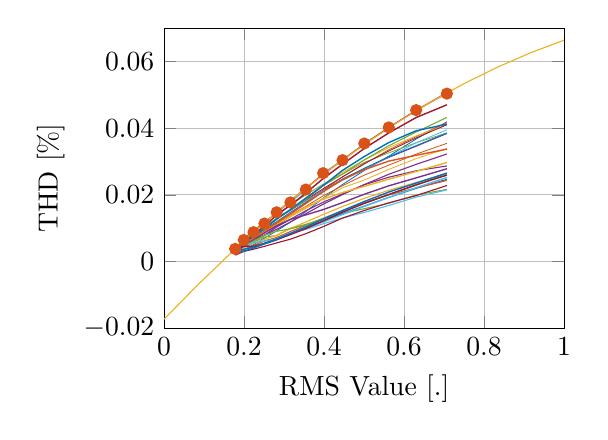
\begin{tikzpicture}

\begin{axis}[%
width=2.0in,
height=1.5in,
at={(0.758in,0.481in)},
scale only axis,
xmin=0,
xmax=1,
xlabel={RMS Value [.]},
xmajorgrids,
ymin=-0.02,
ymax=0.07,
y tick label style={/pgf/number format/fixed},
scaled y ticks = false,
ylabel={THD [\%]},
ymajorgrids,
axis background/.style={fill=white},
legend style={legend cell align=left,align=left,draw=white!15!black},
every axis legend/.code={\let\addlegendentry\relax}
]
\addplot [color=mycolor1,solid,line width=0.3pt]
  table[row sep=crcr]{%
0.177615489572042	0.00205368263706797\\
0.19928785706971	0.00348379415594429\\
0.223604653350506	0.00508702990168937\\
0.250888547527061	0.00703635792364254\\
0.281501580298378	0.00919490750505369\\
0.315849968009946	0.0118280776578328\\
0.354389492897844	0.0149702620002119\\
0.397631551042096	0.0190105008575072\\
0.446149938281945	0.0231148796883891\\
0.500588464138024	0.0273213516432495\\
0.561669494773539	0.0316348501218829\\
0.630203538354371	0.0367512134931775\\
0.7071	0.0419360163557166\\
};
\addlegendentry{290 Hz};

\addplot [color=mycolor2,solid,line width=0.3pt]
  table[row sep=crcr]{%
0.177615489572042	0.00201966696624447\\
0.19928785706971	0.00411726029111224\\
0.223604653350506	0.00648273251531101\\
0.250888547527061	0.00901223787980107\\
0.281501580298378	0.0115823417915366\\
0.315849968009946	0.0143164534502651\\
0.354389492897844	0.0177853771086979\\
0.397631551042096	0.0214229738791661\\
0.446149938281945	0.0253783093031596\\
0.500588464138024	0.0292401659062079\\
0.561669494773539	0.0335348158663386\\
0.630203538354371	0.0374735893582891\\
0.7071	0.0416850833908997\\
};
\addlegendentry{300 Hz};

\addplot [color=mycolor3,solid,line width=0.3pt]
  table[row sep=crcr]{%
0.177615489572042	0.00276228227339719\\
0.19928785706971	0.00496619419005071\\
0.223604653350506	0.00736352721325894\\
0.250888547527061	0.0100072900111444\\
0.281501580298378	0.0125829190383413\\
0.315849968009946	0.0156195220864753\\
0.354389492897844	0.0190985030891485\\
0.397631551042096	0.022861942306566\\
0.446149938281945	0.0268109213801366\\
0.500588464138024	0.0304660572305634\\
0.561669494773539	0.0341819154007577\\
0.630203538354371	0.0376968424032464\\
0.7071	0.041093076359054\\
};
\addlegendentry{310 Hz};

\addplot [color=mycolor4,solid,line width=0.3pt]
  table[row sep=crcr]{%
0.177615489572042	0.00332198388483245\\
0.19928785706971	0.00583290204797817\\
0.223604653350506	0.00798023560699537\\
0.250888547527061	0.0103576210919747\\
0.281501580298378	0.0128699624782435\\
0.315849968009946	0.0153362212352626\\
0.354389492897844	0.0182106985495664\\
0.397631551042096	0.0213557839963975\\
0.446149938281945	0.0246467442844194\\
0.500588464138024	0.0278657889463668\\
0.561669494773539	0.0312073110080607\\
0.630203538354371	0.0345776275591996\\
0.7071	0.038382499555876\\
};
\addlegendentry{320 Hz};

\addplot [color=mycolor5,solid,line width=0.3pt]
  table[row sep=crcr]{%
0.177615489572042	0.00365989016608311\\
0.19928785706971	0.00688650318990293\\
0.223604653350506	0.00935413987411552\\
0.250888547527061	0.0118778547010219\\
0.281501580298378	0.0142251360186623\\
0.315849968009946	0.0169236327061235\\
0.354389492897844	0.0200019570250277\\
0.397631551042096	0.0232059876787582\\
0.446149938281945	0.0262763705142707\\
0.500588464138024	0.0297503637788585\\
0.561669494773539	0.0325988849148936\\
0.630203538354371	0.0356380294920932\\
0.7071	0.0385727568260796\\
};
\addlegendentry{330 Hz};

\addplot [color=mycolor6,solid,line width=0.3pt]
  table[row sep=crcr]{%
0.177615489572042	0.00309118139358734\\
0.19928785706971	0.00544211729577141\\
0.223604653350506	0.00786617703256435\\
0.250888547527061	0.0103271598793815\\
0.281501580298378	0.0129607404726367\\
0.315849968009946	0.0155009199687871\\
0.354389492897844	0.0181829086806762\\
0.397631551042096	0.0212180652914781\\
0.446149938281945	0.0243395567025414\\
0.500588464138024	0.027762186682569\\
0.561669494773539	0.0314022160315982\\
0.630203538354371	0.0356263792989928\\
0.7071	0.0395232752656835\\
};
\addlegendentry{330 Hz};

\addplot [color=mycolor7,solid,line width=0.3pt]
  table[row sep=crcr]{%
0.177615489572042	0.00305062531404795\\
0.19928785706971	0.00561370193192394\\
0.223604653350506	0.00791640400812886\\
0.250888547527061	0.0103282866698295\\
0.281501580298378	0.012658755098407\\
0.315849968009946	0.0154893336961729\\
0.354389492897844	0.0185026092791448\\
0.397631551042096	0.0218452569455399\\
0.446149938281945	0.0254043463494108\\
0.500588464138024	0.0294104915557292\\
0.561669494773539	0.0331388965970306\\
0.630203538354371	0.0370916180311659\\
0.7071	0.0410437813703521\\
};
\addlegendentry{340 Hz};

\addplot [color=mycolor1,solid,line width=0.3pt]
  table[row sep=crcr]{%
0.177615489572042	0.00321858074441963\\
0.19928785706971	0.00546880860272025\\
0.223604653350506	0.00748347106091212\\
0.250888547527061	0.00978410118593892\\
0.281501580298378	0.0119636779532244\\
0.315849968009946	0.0147781066527307\\
0.354389492897844	0.0176754082423151\\
0.397631551042096	0.0208695733119052\\
0.446149938281945	0.0247530068306881\\
0.500588464138024	0.0279846696174777\\
0.561669494773539	0.0314340205918235\\
0.630203538354371	0.0347801659691238\\
0.7071	0.0385695340754765\\
};
\addlegendentry{350 Hz};

\addplot [color=mycolor2,solid,line width=0.3pt]
  table[row sep=crcr]{%
0.177615489572042	0.00303024209309899\\
0.19928785706971	0.00490684929001908\\
0.223604653350506	0.00720859645443171\\
0.250888547527061	0.0090566317478803\\
0.281501580298378	0.0113851664035042\\
0.315849968009946	0.0138725072359532\\
0.354389492897844	0.0165421674653501\\
0.397631551042096	0.0197129630930525\\
0.446149938281945	0.0227713068228533\\
0.500588464138024	0.025929618409697\\
0.561669494773539	0.0289241549089614\\
0.630203538354371	0.0322357019088623\\
0.7071	0.0354580621836129\\
};
\addlegendentry{360 Hz};

\addplot [color=mycolor3,solid,line width=0.3pt]
  table[row sep=crcr]{%
0.177615489572042	0.00316737391020391\\
0.19928785706971	0.0050736205878784\\
0.223604653350506	0.00666525071599896\\
0.250888547527061	0.00866109186311343\\
0.281501580298378	0.0108906038424612\\
0.315849968009946	0.013369731014044\\
0.354389492897844	0.0159159252529334\\
0.397631551042096	0.0189498240409288\\
0.446149938281945	0.0221244979819137\\
0.500588464138024	0.02446866858935\\
0.561669494773539	0.0276427989230973\\
0.630203538354371	0.0308950774949562\\
0.7071	0.0338851556710921\\
};
\addlegendentry{370 Hz};

\addplot [color=mycolor4,solid,line width=0.4pt]
  table[row sep=crcr]{%
0.177615489572042	0.00311058263372326\\
0.19928785706971	0.00487505907896998\\
0.223604653350506	0.00664056716206753\\
0.250888547527061	0.0079151256317128\\
0.281501580298378	0.0103653255308688\\
0.315849968009946	0.0126731402734647\\
0.354389492897844	0.0152288060142371\\
0.397631551042096	0.0177975252361786\\
0.446149938281945	0.0202702171656902\\
0.500588464138024	0.0230554552572268\\
0.561669494773539	0.0252893646468466\\
0.630203538354371	0.0272276411758901\\
0.7071	0.0286718392382435\\
};
\addlegendentry{380 Hz};

\addplot [color=mycolor5,solid,line width=0.4pt]
  table[row sep=crcr]{%
0.177615489572042	0.0030574824635586\\
0.19928785706971	0.00423638477613823\\
0.223604653350506	0.00582439844468536\\
0.250888547527061	0.00733790176943997\\
0.281501580298378	0.00781584671858286\\
0.315849968009946	0.00998201855672553\\
0.354389492897844	0.0111478051200051\\
0.397631551042096	0.0128586213406605\\
0.446149938281945	0.0144102634304792\\
0.500588464138024	0.0158525281390892\\
0.561669494773539	0.017478895858686\\
0.630203538354371	0.0199774169269083\\
0.7071	0.0216450069286161\\
};
\addlegendentry{390 Hz};

\addplot [color=mycolor6,solid,line width=0.4pt]
  table[row sep=crcr]{%
0.177615489572042	0.00281044161822231\\
0.19928785706971	0.00310468459122797\\
0.223604653350506	0.00400566494645231\\
0.250888547527061	0.00548303525693075\\
0.281501580298378	0.00691866640224513\\
0.315849968009946	0.00850278268674514\\
0.354389492897844	0.00962948079841521\\
0.397631551042096	0.0113143304263794\\
0.446149938281945	0.0130470768914605\\
0.500588464138024	0.0147429785110485\\
0.561669494773539	0.0168184720936108\\
0.630203538354371	0.0193280287601095\\
0.7071	0.0214998340471773\\
};
\addlegendentry{400 Hz};

\addplot [color=mycolor7,solid,line width=0.4pt]
  table[row sep=crcr]{%
0.177615489572042	0.00192112562609673\\
0.19928785706971	0.00302915815865948\\
0.223604653350506	0.00369215870291678\\
0.250888547527061	0.00455603095891217\\
0.281501580298378	0.00558961689420662\\
0.315849968009946	0.0067066611763081\\
0.354389492897844	0.00836306752644878\\
0.397631551042096	0.0104630682234524\\
0.446149938281945	0.0130297919530514\\
0.500588464138024	0.0153216722871169\\
0.561669494773539	0.0176202153568934\\
0.630203538354371	0.0197710412752356\\
0.7071	0.022818114950948\\
};
\addlegendentry{410 Hz};

\addplot [color=mycolor1,solid,line width=0.4pt]
  table[row sep=crcr]{%
0.177615489572042	0.00232761785278883\\
0.19928785706971	0.00311741535409893\\
0.223604653350506	0.00402907424175296\\
0.250888547527061	0.00525946929580434\\
0.281501580298378	0.00646252327730194\\
0.315849968009946	0.00822890126576167\\
0.354389492897844	0.0101580475593493\\
0.397631551042096	0.0121676532846197\\
0.446149938281945	0.0143809627560572\\
0.500588464138024	0.0166319103220923\\
0.561669494773539	0.019256656606226\\
0.630203538354371	0.0219459031396591\\
0.7071	0.0246491727540069\\
};
\addlegendentry{420 Hz};

\addplot [color=mycolor2,solid,line width=0.4pt]
  table[row sep=crcr]{%
0.177615489572042	0.00286061274797567\\
0.19928785706971	0.00358740310631459\\
0.223604653350506	0.00479960653408768\\
0.250888547527061	0.00616483575142891\\
0.281501580298378	0.00722959266859313\\
0.315849968009946	0.00899807475905458\\
0.354389492897844	0.0108834649407214\\
0.397631551042096	0.0129565999301207\\
0.446149938281945	0.0152665188676738\\
0.500588464138024	0.0176728698015239\\
0.561669494773539	0.0200135586884394\\
0.630203538354371	0.0220631313185399\\
0.7071	0.0243388739054617\\
};
\addlegendentry{430 Hz};

\addplot [color=mycolor3,solid,line width=0.4pt]
  table[row sep=crcr]{%
0.177615489572042	0.00305272742837913\\
0.19928785706971	0.00408919116272087\\
0.223604653350506	0.0054566601416978\\
0.250888547527061	0.00662255878179251\\
0.281501580298378	0.00789226609825561\\
0.315849968009946	0.00993640142054062\\
0.354389492897844	0.0118465098067896\\
0.397631551042096	0.0141004956552334\\
0.446149938281945	0.0165062066466515\\
0.500588464138024	0.0189565983740301\\
0.561669494773539	0.021364696374166\\
0.630203538354371	0.023724845472541\\
0.7071	0.0262932237760931\\
};
\addlegendentry{440 Hz};

\addplot [color=mycolor4,solid,line width=0.4pt]
  table[row sep=crcr]{%
0.177615489572042	0.00364103239690753\\
0.19928785706971	0.00493948403439657\\
0.223604653350506	0.00635195983820561\\
0.250888547527061	0.00786141697071262\\
0.281501580298378	0.00968360118244828\\
0.315849968009946	0.0118655160202202\\
0.354389492897844	0.014356726848741\\
0.397631551042096	0.0172026105956467\\
0.446149938281945	0.0201045569745367\\
0.500588464138024	0.0230836533409526\\
0.561669494773539	0.0261745052597013\\
0.630203538354371	0.0291610635155859\\
0.7071	0.032265307467225\\
};
\addlegendentry{450 Hz};

\addplot [color=mycolor5,solid,line width=0.4pt]
  table[row sep=crcr]{%
0.177615489572042	0.0037172905844415\\
0.19928785706971	0.00579880788496196\\
0.223604653350506	0.00786561596743004\\
0.250888547527061	0.0102901224230776\\
0.281501580298378	0.0129411963825515\\
0.315849968009946	0.0154520583739255\\
0.354389492897844	0.0186335932385422\\
0.397631551042096	0.022757158187896\\
0.446149938281945	0.0262171215828906\\
0.500588464138024	0.0304983875140885\\
0.561669494773539	0.0347312513207695\\
0.630203538354371	0.0388639991368012\\
0.7071	0.043236756125032\\
};
\addlegendentry{460 Hz};

\addplot [color=mycolor6,solid,line width=0.4pt]
  table[row sep=crcr]{%
0.177615489572042	0.00380008783125512\\
0.19928785706971	0.00646994838397832\\
0.223604653350506	0.00880949534573053\\
0.250888547527061	0.0113927694174674\\
0.281501580298378	0.0147702628429983\\
0.315849968009946	0.0177378174116172\\
0.354389492897844	0.0216019956642725\\
0.397631551042096	0.0265158531779721\\
0.446149938281945	0.0304200469565269\\
0.500588464138024	0.0354192280754121\\
0.561669494773539	0.0402457845477729\\
0.630203538354371	0.0454282983702959\\
0.7071	0.0503827333185046\\
};
\addlegendentry{470 Hz};

\addplot [color=mycolor7,solid,line width=0.5pt]
  table[row sep=crcr]{%
0.177615489572042	0.00355446038037562\\
0.19928785706971	0.00599342833629029\\
0.223604653350506	0.00806899794207545\\
0.250888547527061	0.0106193769345377\\
0.281501580298378	0.0139563395737668\\
0.315849968009946	0.0168878518941196\\
0.354389492897844	0.02055072028397\\
0.397631551042096	0.0248776009742118\\
0.446149938281945	0.0291834095241609\\
0.500588464138024	0.0339332813532551\\
0.561669494773539	0.0385825826571098\\
0.630203538354371	0.0432071415486898\\
0.7071	0.0470282209816381\\
};
\addlegendentry{480 Hz};

\addplot [color=mycolor1,solid,line width=0.5pt]
  table[row sep=crcr]{%
0.177615489572042	0.00345657307501929\\
0.19928785706971	0.00552323545414325\\
0.223604653350506	0.00747701461603942\\
0.250888547527061	0.00978322910023166\\
0.281501580298378	0.0127990738171938\\
0.315849968009946	0.0156059740615896\\
0.354389492897844	0.0190249407731675\\
0.397631551042096	0.0227967208688532\\
0.446149938281945	0.0273586684379134\\
0.500588464138024	0.0315162195415954\\
0.561669494773539	0.0356992722998556\\
0.630203538354371	0.0392466627969218\\
0.7071	0.0412162211106101\\
};
\addlegendentry{490 Hz};

\addplot [color=mycolor2,solid,line width=0.5pt]
  table[row sep=crcr]{%
0.177615489572042	0.00323086949030111\\
0.19928785706971	0.00513039606826508\\
0.223604653350506	0.00700100902764595\\
0.250888547527061	0.00915583476880373\\
0.281501580298378	0.0116428005335728\\
0.315849968009946	0.0142773666178676\\
0.354389492897844	0.0174132093164672\\
0.397631551042096	0.0209796330053973\\
0.446149938281945	0.0245593521477064\\
0.500588464138024	0.0275649892483374\\
0.561669494773539	0.0301278744665206\\
0.630203538354371	0.0318751687557911\\
0.7071	0.0337207690791282\\
};
\addlegendentry{500 Hz};

\addplot [color=mycolor3,solid,line width=0.5pt]
  table[row sep=crcr]{%
0.177615489572042	0.00323387647581326\\
0.19928785706971	0.0050702045508761\\
0.223604653350506	0.00672061757976626\\
0.250888547527061	0.00873415495339072\\
0.281501580298378	0.0110510495665548\\
0.315849968009946	0.0136704807329027\\
0.354389492897844	0.0162783304848873\\
0.397631551042096	0.018736759217012\\
0.446149938281945	0.0206962374906118\\
0.500588464138024	0.0225609134405443\\
0.561669494773539	0.0246962331391943\\
0.630203538354371	0.0270180165309514\\
0.7071	0.0297235046549367\\
};
\addlegendentry{510 Hz};

\addplot [color=mycolor4,solid,line width=0.5pt]
  table[row sep=crcr]{%
0.177615489572042	0.00328503475860528\\
0.19928785706971	0.0049775499970034\\
0.223604653350506	0.00655180007885434\\
0.250888547527061	0.00859281000397108\\
0.281501580298378	0.0107713038010384\\
0.315849968009946	0.0126353071787087\\
0.354389492897844	0.0139987262818764\\
0.397631551042096	0.0155787281416255\\
0.446149938281945	0.0176898297107059\\
0.500588464138024	0.0201903661928242\\
0.561669494773539	0.0227190707976797\\
0.630203538354371	0.0250990513111019\\
0.7071	0.0278407297846789\\
};
\addlegendentry{520 Hz};

\addplot [color=mycolor5,solid]
  table[row sep=crcr]{%
0.177615489572042	0.00302425179306022\\
0.19928785706971	0.00459392778519979\\
0.223604653350506	0.00614655726276875\\
0.250888547527061	0.00791018201764182\\
0.281501580298378	0.00905979684556054\\
0.315849968009946	0.00982761302865274\\
0.354389492897844	0.0109894772086868\\
0.397631551042096	0.012838673527107\\
0.446149938281945	0.0151655595584971\\
0.500588464138024	0.0174767892394402\\
0.561669494773539	0.0200070196541781\\
0.630203538354371	0.0228885983398539\\
0.7071	0.0263726272672322\\
};
\addlegendentry{530 Hz};

\addplot [color=mycolor6,solid,line width=0.5pt]
  table[row sep=crcr]{%
0.177615489572042	0.00275707208633809\\
0.19928785706971	0.00442064809402789\\
0.223604653350506	0.00571949756958684\\
0.250888547527061	0.00611133160155234\\
0.281501580298378	0.00678891125746833\\
0.315849968009946	0.00834568723120321\\
0.354389492897844	0.00994240048974564\\
0.397631551042096	0.0118697227518085\\
0.446149938281945	0.0141146295731797\\
0.500588464138024	0.0165431707814268\\
0.561669494773539	0.01924106571207\\
0.630203538354371	0.022164929525125\\
0.7071	0.025215199611294\\
};
\addlegendentry{540 Hz};

\addplot [color=mycolor7,solid,line width=0.5pt]
  table[row sep=crcr]{%
0.177615489572042	0.00292427841677326\\
0.19928785706971	0.00463268799971246\\
0.223604653350506	0.00457499075408101\\
0.250888547527061	0.00546965240792525\\
0.281501580298378	0.00661546990280243\\
0.315849968009946	0.00808914508954947\\
0.354389492897844	0.00990258487034653\\
0.397631551042096	0.0121799009415681\\
0.446149938281945	0.0148313712500093\\
0.500588464138024	0.017435776573817\\
0.561669494773539	0.0201311079173622\\
0.630203538354371	0.0230366549514656\\
0.7071	0.025928377302547\\
};
\addlegendentry{550 Hz};

\addplot [color=mycolor1,solid,line width=0.5pt]
  table[row sep=crcr]{%
0.177615489572042	0.00329009241708662\\
0.19928785706971	0.00361089368263843\\
0.223604653350506	0.00434114332668855\\
0.250888547527061	0.00534277101473772\\
0.281501580298378	0.00673325799903008\\
0.315849968009946	0.00843963748825095\\
0.354389492897844	0.010419423532532\\
0.397631551042096	0.0127220671440617\\
0.446149938281945	0.0153009020248404\\
0.500588464138024	0.0180144629947333\\
0.561669494773539	0.02084805917905\\
0.630203538354371	0.0235415129000979\\
0.7071	0.0265515454426621\\
};
\addlegendentry{560 Hz};

\addplot [color=mycolor2,only marks,mark=*,mark options={solid}]
  table[row sep=crcr]{%
0.177615489572042	0.00380008783125512\\
0.19928785706971	0.00646994838397832\\
0.223604653350506	0.00880949534573053\\
0.250888547527061	0.0113927694174674\\
0.281501580298378	0.0147702628429983\\
0.315849968009946	0.0177378174116172\\
0.354389492897844	0.0216019956642725\\
0.397631551042096	0.0265158531779721\\
0.446149938281945	0.0304200469565269\\
0.500588464138024	0.0354192280754121\\
0.561669494773539	0.0402457845477729\\
0.630203538354371	0.0454282983702959\\
0.7071	0.0503827333185046\\
};
\addlegendentry{data};

\addplot [color=red,solid]
  table[row sep=crcr]{%
0.177615489572042	0.00372803154716359\\
0.17814497408247	0.00378672984091505\\
0.178674458592898	0.00384540453161158\\
0.179203943103326	0.0039040556192532\\
0.179733427613754	0.0039626831038399\\
0.180262912124182	0.00402128698537166\\
0.18079239663461	0.00407986726384851\\
0.181321881145038	0.00413842393927043\\
0.181851365655466	0.00419695701163743\\
0.182380850165894	0.0042554664809495\\
0.182910334676322	0.00431395234720666\\
0.18343981918675	0.00437241461040888\\
0.183969303697178	0.00443085327055619\\
0.184498788207606	0.00448926832764857\\
0.185028272718034	0.00454765978168603\\
0.185557757228462	0.00460602763266857\\
0.18608724173889	0.00466437188059618\\
0.186616726249318	0.00472269252546887\\
0.187146210759746	0.00478098956728663\\
0.187675695270174	0.00483926300604947\\
0.188205179780602	0.00489751284175739\\
0.18873466429103	0.00495573907441039\\
0.189264148801457	0.00501394170400846\\
0.189793633311885	0.00507212073055161\\
0.190323117822313	0.00513027615403983\\
0.190852602332741	0.00518840797447314\\
0.191382086843169	0.00524651619185151\\
0.191911571353597	0.00530460080617497\\
0.192441055864025	0.0053626618174435\\
0.192970540374453	0.00542069922565711\\
0.193500024884881	0.0054787130308158\\
0.194029509395309	0.00553670323291956\\
0.194558993905737	0.00559466983196839\\
0.195088478416165	0.00565261282796231\\
0.195617962926593	0.0057105322209013\\
0.196147447437021	0.00576842801078537\\
0.196676931947449	0.00582630019761451\\
0.197206416457877	0.00588414878138874\\
0.197735900968305	0.00594197376210803\\
0.198265385478733	0.00599977513977241\\
0.198794869989161	0.00605755291438186\\
0.19928785706971	0.00611132684147301\\
0.199324354499589	0.00611530708593639\\
0.199853839010017	0.00617303765443599\\
0.200383323520445	0.00623074461988068\\
0.200912808030873	0.00628842798227043\\
0.201442292541301	0.00634608774160527\\
0.201971777051728	0.00640372389788518\\
0.202501261562156	0.00646133645111017\\
0.203030746072584	0.00651892540128023\\
0.203560230583012	0.00657649074839537\\
0.20408971509344	0.00663403249245559\\
0.204619199603868	0.00669155063346089\\
0.205148684114296	0.00674904517141126\\
0.205678168624724	0.00680651610630671\\
0.206207653135152	0.00686396343814723\\
0.20673713764558	0.00692138716693283\\
0.207266622156008	0.00697878729266351\\
0.207796106666436	0.00703616381533926\\
0.208325591176864	0.0070935167349601\\
0.208855075687292	0.007150846051526\\
0.20938456019772	0.00720815176503699\\
0.209914044708148	0.00726543387549305\\
0.210443529218576	0.00732269238289419\\
0.210973013729004	0.0073799272872404\\
0.211502498239432	0.00743713858853169\\
0.21203198274986	0.00749432628676806\\
0.212561467260288	0.0075514903819495\\
0.213090951770716	0.00760863087407603\\
0.213620436281144	0.00766574776314763\\
0.214149920791571	0.0077228410491643\\
0.214679405301999	0.00777991073212605\\
0.215208889812427	0.00783695681203288\\
0.215738374322855	0.00789397928888478\\
0.216267858833283	0.00795097816268176\\
0.216797343343711	0.00800795343342382\\
0.217326827854139	0.00806490510111095\\
0.217856312364567	0.00812183316574317\\
0.218385796874995	0.00817873762732045\\
0.218915281385423	0.00823561848584282\\
0.219444765895851	0.00829247574131026\\
0.219974250406279	0.00834930939372278\\
0.220503734916707	0.00840611944308037\\
0.221033219427135	0.00846290588938304\\
0.221562703937563	0.00851966873263079\\
0.222092188447991	0.00857640797282361\\
0.222621672958419	0.00863312360996151\\
0.223151157468847	0.00868981564404449\\
0.223604653350506	0.00873835279228205\\
0.223680641979275	0.00874648407507254\\
0.224210126489703	0.00880312890304568\\
0.224739611000131	0.00885975012796389\\
0.225269095510559	0.00891634774982716\\
0.225798580020987	0.00897292176863553\\
0.226328064531414	0.00902947218438897\\
0.226857549041842	0.00908599899708748\\
0.22738703355227	0.00914250220673107\\
0.227916518062698	0.00919898181331974\\
0.228446002573126	0.00925543781685348\\
0.228975487083554	0.0093118702173323\\
0.229504971593982	0.0093682790147562\\
0.23003445610441	0.00942466420912517\\
0.230563940614838	0.00948102580043922\\
0.231093425125266	0.00953736378869835\\
0.231622909635694	0.00959367817390256\\
0.232152394146122	0.00964996895605183\\
0.23268187865655	0.00970623613514619\\
0.233211363166978	0.00976247971118563\\
0.233740847677406	0.00981869968417013\\
0.234270332187834	0.00987489605409972\\
0.234799816698262	0.00993106882097439\\
0.23532930120869	0.00998721798479412\\
0.235858785719118	0.0100433435455589\\
0.236388270229546	0.0100994455032688\\
0.236917754739974	0.0101555238579238\\
0.237447239250402	0.0102115786095239\\
0.23797672376083	0.010267609758069\\
0.238506208271258	0.0103236173035592\\
0.239035692781685	0.0103796012459945\\
0.239565177292113	0.0104355615853748\\
0.240094661802541	0.0104914983217002\\
0.240624146312969	0.0105474114549707\\
0.241153630823397	0.0106033009851863\\
0.241683115333825	0.010659166912347\\
0.242212599844253	0.0107150092364527\\
0.242742084354681	0.0107708279575035\\
0.243271568865109	0.0108266230754994\\
0.243801053375537	0.0108823945904404\\
0.244330537885965	0.0109381425023264\\
0.244860022396393	0.0109938668111576\\
0.245389506906821	0.0110495675169338\\
0.245918991417249	0.011105244619655\\
0.246448475927677	0.0111608981193214\\
0.246977960438105	0.0112165280159328\\
0.247507444948533	0.0112721343094893\\
0.248036929458961	0.0113277169999909\\
0.248566413969389	0.0113832760874375\\
0.249095898479817	0.0114388115718293\\
0.249625382990245	0.0114943234531661\\
0.250154867500673	0.011549811731448\\
0.250684352011101	0.0116052764066749\\
0.250888547527061	0.0116266600328014\\
0.251213836521529	0.011660717478847\\
0.251743321031956	0.0117161349479641\\
0.252272805542384	0.0117715288140263\\
0.252802290052812	0.0118268990770336\\
0.25333177456324	0.0118822457369859\\
0.253861259073668	0.0119375687938833\\
0.254390743584096	0.0119928682477258\\
0.254920228094524	0.0120481440985134\\
0.255449712604952	0.0121033963462461\\
0.25597919711538	0.0121586249909238\\
0.256508681625808	0.0122138300325466\\
0.257038166136236	0.0122690114711145\\
0.257567650646664	0.0123241693066274\\
0.258097135157092	0.0123793035390855\\
0.25862661966752	0.0124344141684886\\
0.259156104177948	0.0124895011948368\\
0.259685588688376	0.01254456461813\\
0.260215073198804	0.0125996044383684\\
0.260744557709232	0.0126546206555518\\
0.26127404221966	0.0127096132696803\\
0.261803526730088	0.0127645822807539\\
0.262333011240516	0.0128195276887725\\
0.262862495750944	0.0128744494937362\\
0.263391980261372	0.012929347695645\\
0.263921464771799	0.0129842222944989\\
0.264450949282227	0.0130390732902979\\
0.264980433792655	0.0130939006830419\\
0.265509918303083	0.013148704472731\\
0.266039402813511	0.0132034846593652\\
0.266568887323939	0.0132582412429445\\
0.267098371834367	0.0133129742234688\\
0.267627856344795	0.0133676836009382\\
0.268157340855223	0.0134223693753527\\
0.268686825365651	0.0134770315467123\\
0.269216309876079	0.0135316701150169\\
0.269745794386507	0.0135862850802667\\
0.270275278896935	0.0136408764424615\\
0.270804763407363	0.0136954442016013\\
0.271334247917791	0.0137499883576863\\
0.271863732428219	0.0138045089107163\\
0.272393216938647	0.0138590058606914\\
0.272922701449075	0.0139134792076116\\
0.273452185959503	0.0139679289514769\\
0.273981670469931	0.0140223550922872\\
0.274511154980359	0.0140767576300426\\
0.275040639490787	0.0141311365647431\\
0.275570124001215	0.0141854918963887\\
0.276099608511643	0.0142398236249793\\
0.27662909302207	0.014294131750515\\
0.277158577532498	0.0143484162729958\\
0.277688062042926	0.0144026771924217\\
0.278217546553354	0.0144569145087926\\
0.278747031063782	0.0145111282221087\\
0.27927651557421	0.0145653183323698\\
0.279806000084638	0.014619484839576\\
0.280335484595066	0.0146736277437272\\
0.280864969105494	0.0147277470448235\\
0.281394453615922	0.014781842742865\\
0.281501580298378	0.0147927846543008\\
0.28192393812635	0.0148359148378514\\
0.282453422636778	0.014889963329783\\
0.282982907147206	0.0149439882186596\\
0.283512391657634	0.0149979895044813\\
0.284041876168062	0.0150519671872481\\
0.28457136067849	0.01510592126696\\
0.285100845188918	0.015159851743617\\
0.285630329699346	0.015213758617219\\
0.286159814209774	0.0152676418877661\\
0.286689298720202	0.0153215015552583\\
0.28721878323063	0.0153753376196955\\
0.287748267741058	0.0154291500810778\\
0.288277752251486	0.0154829389394052\\
0.288807236761913	0.0155367041946777\\
0.289336721272341	0.0155904458468953\\
0.289866205782769	0.0156441638960579\\
0.290395690293197	0.0156978583421656\\
0.290925174803625	0.0157515291852184\\
0.291454659314053	0.0158051764252163\\
0.291984143824481	0.0158588000621592\\
0.292513628334909	0.0159124000960472\\
0.293043112845337	0.0159659765268803\\
0.293572597355765	0.0160195293546585\\
0.294102081866193	0.0160730585793817\\
0.294631566376621	0.0161265642010501\\
0.295161050887049	0.0161800462196635\\
0.295690535397477	0.016233504635222\\
0.296220019907905	0.0162869394477255\\
0.296749504418333	0.0163403506571741\\
0.297278988928761	0.0163937382635679\\
0.297808473439189	0.0164471022669066\\
0.298337957949617	0.0165004426671905\\
0.298867442460045	0.0165537594644194\\
0.299396926970473	0.0166070526585935\\
0.299926411480901	0.0166603222497126\\
0.300455895991329	0.0167135682377767\\
0.300985380501756	0.016766790622786\\
0.301514865012184	0.0168199894047403\\
0.302044349522612	0.0168731645836397\\
0.30257383403304	0.0169263161594842\\
0.303103318543468	0.0169794441322737\\
0.303632803053896	0.0170325485020083\\
0.304162287564324	0.017085629268688\\
0.304691772074752	0.0171386864323128\\
0.30522125658518	0.0171917199928827\\
0.305750741095608	0.0172447299503976\\
0.306280225606036	0.0172977163048576\\
0.306809710116464	0.0173506790562627\\
0.307339194626892	0.0174036182046129\\
0.30786867913732	0.0174565337499081\\
0.308398163647748	0.0175094256921484\\
0.308927648158176	0.0175622940313338\\
0.309457132668604	0.0176151387674643\\
0.309986617179032	0.0176679599005398\\
0.31051610168946	0.0177207574305605\\
0.311045586199888	0.0177735313575262\\
0.311575070710316	0.017826281681437\\
0.312104555220744	0.0178790084022928\\
0.312634039731172	0.0179317115200937\\
0.3131635242416	0.0179843910348397\\
0.313693008752027	0.0180370469465308\\
0.314222493262455	0.018089679255167\\
0.314751977772883	0.0181422879607482\\
0.315281462283311	0.0181948730632745\\
0.315810946793739	0.0182474345627459\\
0.315849968009946	0.0182513072335166\\
0.316340431304167	0.0182999724591624\\
0.316869915814595	0.018352486752524\\
0.317399400325023	0.0184049774428306\\
0.317928884835451	0.0184574445300823\\
0.318458369345879	0.018509888014279\\
0.318987853856307	0.0185623078954209\\
0.319517338366735	0.0186147041735078\\
0.320046822877163	0.0186670768485398\\
0.320576307387591	0.0187194259205169\\
0.321105791898019	0.0187717513894391\\
0.321635276408447	0.0188240532553063\\
0.322164760918875	0.0188763315181186\\
0.322694245429303	0.018928586177876\\
0.323223729939731	0.0189808172345785\\
0.323753214450159	0.019033024688226\\
0.324282698960587	0.0190852085388186\\
0.324812183471015	0.0191373687863563\\
0.325341667981443	0.0191895054308391\\
0.32587115249187	0.0192416184722669\\
0.326400637002298	0.0192937079106399\\
0.326930121512726	0.0193457737459579\\
0.327459606023154	0.0193978159782209\\
0.327989090533582	0.0194498346074291\\
0.32851857504401	0.0195018296335823\\
0.329048059554438	0.0195538010566806\\
0.329577544064866	0.019605748876724\\
0.330107028575294	0.0196576730937125\\
0.330636513085722	0.019709573707646\\
0.33116599759615	0.0197614507185246\\
0.331695482106578	0.0198133041263483\\
0.332224966617006	0.0198651339311171\\
0.332754451127434	0.0199169401328309\\
0.333283935637862	0.0199687227314898\\
0.33381342014829	0.0200204817270938\\
0.334342904658718	0.0200722171196429\\
0.334872389169146	0.0201239289091371\\
0.335401873679574	0.0201756170955763\\
0.335931358190002	0.0202272816789606\\
0.33646084270043	0.02027892265929\\
0.336990327210858	0.0203305400365644\\
0.337519811721286	0.020382133810784\\
0.338049296231714	0.0204337039819486\\
0.338578780742141	0.0204852505500583\\
0.339108265252569	0.020536773515113\\
0.339637749762997	0.0205882728771129\\
0.340167234273425	0.0206397486360578\\
0.340696718783853	0.0206912007919478\\
0.341226203294281	0.0207426293447828\\
0.341755687804709	0.020794034294563\\
0.342285172315137	0.0208454156412882\\
0.342814656825565	0.0208967733849585\\
0.343344141335993	0.0209481075255739\\
0.343873625846421	0.0209994180631343\\
0.344403110356849	0.0210507049976399\\
0.344932594867277	0.0211019683290905\\
0.345462079377705	0.0211532080574862\\
0.345991563888133	0.0212044241828269\\
0.346521048398561	0.0212556167051128\\
0.347050532908989	0.0213067856243437\\
0.347580017419417	0.0213579309405197\\
0.348109501929845	0.0214090526536407\\
0.348638986440273	0.0214601507637069\\
0.349168470950701	0.0215112252707181\\
0.349697955461129	0.0215622761746744\\
0.350227439971557	0.0216133034755758\\
0.350756924481984	0.0216643071734222\\
0.351286408992412	0.0217152872682137\\
0.35181589350284	0.0217662437599503\\
0.352345378013268	0.021817176648632\\
0.352874862523696	0.0218680859342588\\
0.353404347034124	0.0219189716168306\\
0.353933831544552	0.0219698336963475\\
0.354389492897844	0.0220135854554329\\
0.35446331605498	0.0220206721728095\\
0.354992800565408	0.0220714870462166\\
0.355522285075836	0.0221222783165687\\
0.356051769586264	0.0221730459838659\\
0.356581254096692	0.0222237900481082\\
0.35711073860712	0.0222745105092956\\
0.357640223117548	0.022325207367428\\
0.358169707627976	0.0223758806225056\\
0.358699192138404	0.0224265302745282\\
0.359228676648832	0.0224771563234958\\
0.35975816115926	0.0225277587694086\\
0.360287645669688	0.0225783376122664\\
0.360817130180116	0.0226288928520693\\
0.361346614690544	0.0226794244888173\\
0.361876099200972	0.0227299325225104\\
0.3624055837114	0.0227804169531485\\
0.362935068221828	0.0228308777807317\\
0.363464552732255	0.02288131500526\\
0.363994037242683	0.0229317286267334\\
0.364523521753111	0.0229821186451518\\
0.365053006263539	0.0230324850605153\\
0.365582490773967	0.0230828278728239\\
0.366111975284395	0.0231331470820776\\
0.366641459794823	0.0231834426882763\\
0.367170944305251	0.0232337146914202\\
0.367700428815679	0.0232839630915091\\
0.368229913326107	0.0233341878885431\\
0.368759397836535	0.0233843890825221\\
0.369288882346963	0.0234345666734462\\
0.369818366857391	0.0234847206613155\\
0.370347851367819	0.0235348510461297\\
0.370877335878247	0.0235849578278891\\
0.371406820388675	0.0236350410065935\\
0.371936304899103	0.0236851005822431\\
0.372465789409531	0.0237351365548376\\
0.372995273919959	0.0237851489243773\\
0.373524758430387	0.0238351376908621\\
0.374054242940815	0.0238851028542919\\
0.374583727451243	0.0239350444146668\\
0.375113211961671	0.0239849623719868\\
0.375642696472098	0.0240348567262518\\
0.376172180982526	0.0240847274774619\\
0.376701665492954	0.0241345746256171\\
0.377231150003382	0.0241843981707174\\
0.37776063451381	0.0242341981127628\\
0.378290119024238	0.0242839744517532\\
0.378819603534666	0.0243337271876887\\
0.379349088045094	0.0243834563205693\\
0.379878572555522	0.024433161850395\\
0.38040805706595	0.0244828437771657\\
0.380937541576378	0.0245325021008815\\
0.381467026086806	0.0245821368215424\\
0.381996510597234	0.0246317479391484\\
0.382525995107662	0.0246813354536995\\
0.38305547961809	0.0247308993651956\\
0.383584964128518	0.0247804396736368\\
0.384114448638946	0.0248299563790231\\
0.384643933149374	0.0248794494813544\\
0.385173417659802	0.0249289189806309\\
0.38570290217023	0.0249783648768524\\
0.386232386680658	0.025027787170019\\
0.386761871191086	0.0250771858601306\\
0.387291355701514	0.0251265609471874\\
0.387820840211942	0.0251759124311892\\
0.388350324722369	0.0252252403121361\\
0.388879809232797	0.025274544590028\\
0.389409293743225	0.0253238252648651\\
0.389938778253653	0.0253730823366472\\
0.390468262764081	0.0254223158053744\\
0.390997747274509	0.0254715256710467\\
0.391527231784937	0.025520711933664\\
0.392056716295365	0.0255698745932265\\
0.392586200805793	0.025619013649734\\
0.393115685316221	0.0256681291031865\\
0.393645169826649	0.0257172209535842\\
0.394174654337077	0.0257662892009269\\
0.394704138847505	0.0258153338452147\\
0.395233623357933	0.0258643548864476\\
0.395763107868361	0.0259133523246256\\
0.396292592378789	0.0259623261597486\\
0.396822076889217	0.0260112763918168\\
0.397351561399645	0.02606020302083\\
0.397631551042096	0.0260860657183837\\
0.397881045910073	0.0261091060467882\\
0.398410530420501	0.0261579854696916\\
0.398940014930929	0.02620684128954\\
0.399469499441357	0.0262556735063335\\
0.399998983951785	0.0263044821200721\\
0.400528468462212	0.0263532671307557\\
0.40105795297264	0.0264020285383845\\
0.401587437483068	0.0264507663429583\\
0.402116921993496	0.0264994805444772\\
0.402646406503924	0.0265481711429411\\
0.403175891014352	0.0265968381383502\\
0.40370537552478	0.0266454815307043\\
0.404234860035208	0.0266941013200035\\
0.404764344545636	0.0267426975062477\\
0.405293829056064	0.0267912700894371\\
0.405823313566492	0.0268398190695715\\
0.40635279807692	0.026888344446651\\
0.406882282587348	0.0269368462206756\\
0.407411767097776	0.0269853243916452\\
0.407941251608204	0.02703377895956\\
0.408470736118632	0.0270822099244197\\
0.40900022062906	0.0271306172862246\\
0.409529705139488	0.0271790010449746\\
0.410059189649916	0.0272273612006696\\
0.410588674160344	0.0272756977533097\\
0.411118158670772	0.0273240107028949\\
0.4116476431812	0.0273723000494252\\
0.412177127691628	0.0274205657929005\\
0.412706612202056	0.027468807933321\\
0.413236096712484	0.0275170264706864\\
0.413765581222911	0.027565221404997\\
0.414295065733339	0.0276133927362527\\
0.414824550243767	0.0276615404644534\\
0.415354034754195	0.0277096645895992\\
0.415883519264623	0.0277577651116901\\
0.416413003775051	0.027805842030726\\
0.416942488285479	0.0278538953467071\\
0.417471972795907	0.0279019250596332\\
0.418001457306335	0.0279499311695043\\
0.418530941816763	0.0279979136763206\\
0.419060426327191	0.0280458725800819\\
0.419589910837619	0.0280938078807884\\
0.420119395348047	0.0281417195784398\\
0.420648879858475	0.0281896076730364\\
0.421178364368903	0.0282374721645781\\
0.421707848879331	0.0282853130530648\\
0.422237333389759	0.0283331303384966\\
0.422766817900187	0.0283809240208735\\
0.423296302410615	0.0284286941001954\\
0.423825786921043	0.0284764405764624\\
0.424355271431471	0.0285241634496745\\
0.424884755941899	0.0285718627198317\\
0.425414240452327	0.028619538386934\\
0.425943724962754	0.0286671904509813\\
0.426473209473182	0.0287148189119737\\
0.42700269398361	0.0287624237699112\\
0.427532178494038	0.0288100050247938\\
0.428061663004466	0.0288575626766214\\
0.428591147514894	0.0289050967253941\\
0.429120632025322	0.0289526071711119\\
0.42965011653575	0.0290000940137748\\
0.430179601046178	0.0290475572533827\\
0.430709085556606	0.0290949968899358\\
0.431238570067034	0.0291424129234339\\
0.431768054577462	0.029189805353877\\
0.43229753908789	0.0292371741812653\\
0.432827023598318	0.0292845194055986\\
0.433356508108746	0.029331841026877\\
0.433885992619174	0.0293791390451005\\
0.434415477129602	0.0294264134602691\\
0.43494496164003	0.0294736642723827\\
0.435474446150458	0.0295208914814414\\
0.436003930660886	0.0295680950874452\\
0.436533415171314	0.0296152750903941\\
0.437062899681742	0.029662431490288\\
0.43759238419217	0.029709564287127\\
0.438121868702598	0.0297566734809111\\
0.438651353213025	0.0298037590716403\\
0.439180837723453	0.0298508210593146\\
0.439710322233881	0.0298978594439339\\
0.440239806744309	0.0299448742254983\\
0.440769291254737	0.0299918654040078\\
0.441298775765165	0.0300388329794623\\
0.441828260275593	0.030085776951862\\
0.442357744786021	0.0301326973212067\\
0.442887229296449	0.0301795940874965\\
0.443416713806877	0.0302264672507313\\
0.443946198317305	0.0302733168109113\\
0.444475682827733	0.0303201427680363\\
0.445005167338161	0.0303669451221064\\
0.445534651848589	0.0304137238731215\\
0.446064136359017	0.0304604790210818\\
0.446149938281945	0.0304680533784807\\
0.446593620869445	0.0305072105659871\\
0.447123105379873	0.0305539185078375\\
0.447652589890301	0.030600602846633\\
0.448182074400729	0.0306472635823735\\
0.448711558911157	0.0306939007150592\\
0.449241043421585	0.0307405142446899\\
0.449770527932013	0.0307871041712657\\
0.450300012442441	0.0308336704947865\\
0.450829496952868	0.0308802132152525\\
0.451358981463296	0.0309267323326635\\
0.451888465973724	0.0309732278470196\\
0.452417950484152	0.0310196997583207\\
0.45294743499458	0.031066148066567\\
0.453476919505008	0.0311125727717583\\
0.454006404015436	0.0311589738738947\\
0.454535888525864	0.0312053513729762\\
0.455065373036292	0.0312517052690027\\
0.45559485754672	0.0312980355619743\\
0.456124342057148	0.031344342251891\\
0.456653826567576	0.0313906253387528\\
0.457183311078004	0.0314368848225597\\
0.457712795588432	0.0314831207033116\\
0.45824228009886	0.0315293329810086\\
0.458771764609288	0.0315755216556507\\
0.459301249119716	0.0316216867272379\\
0.459830733630144	0.0316678281957701\\
0.460360218140572	0.0317139460612474\\
0.460889702651	0.0317600403236698\\
0.461419187161428	0.0318061109830373\\
0.461948671671856	0.0318521580393498\\
0.462478156182284	0.0318981814926075\\
0.463007640692712	0.0319441813428102\\
0.463537125203139	0.0319901575899579\\
0.464066609713567	0.0320361102340508\\
0.464596094223995	0.0320820392750887\\
0.465125578734423	0.0321279447130717\\
0.465655063244851	0.0321738265479998\\
0.466184547755279	0.032219684779873\\
0.466714032265707	0.0322655194086912\\
0.467243516776135	0.0323113304344545\\
0.467773001286563	0.0323571178571629\\
0.468302485796991	0.0324028816768164\\
0.468831970307419	0.0324486218934149\\
0.469361454817847	0.0324943385069585\\
0.469890939328275	0.0325400315174472\\
0.470420423838703	0.032585700924881\\
0.470949908349131	0.0326313467292599\\
0.471479392859559	0.0326769689305838\\
0.472008877369987	0.0327225675288528\\
0.472538361880415	0.0327681425240669\\
0.473067846390843	0.032813693916226\\
0.473597330901271	0.0328592217053302\\
0.474126815411699	0.0329047258913795\\
0.474656299922127	0.0329502064743739\\
0.475185784432555	0.0329956634543134\\
0.475715268942982	0.0330410968311979\\
0.47624475345341	0.0330865066050276\\
0.476774237963838	0.0331318927758022\\
0.477303722474266	0.033177255343522\\
0.477833206984694	0.0332225943081869\\
0.478362691495122	0.0332679096697968\\
0.47889217600555	0.0333132014283518\\
0.479421660515978	0.0333584695838519\\
0.479951145026406	0.033403714136297\\
0.480480629536834	0.0334489350856872\\
0.481010114047262	0.0334941324320225\\
0.48153959855769	0.0335393061753029\\
0.482069083068118	0.0335844563155284\\
0.482598567578546	0.0336295828526989\\
0.483128052088974	0.0336746857868145\\
0.483657536599402	0.0337197651178752\\
0.48418702110983	0.033764820845881\\
0.484716505620258	0.0338098529708318\\
0.485245990130686	0.0338548614927277\\
0.485775474641114	0.0338998464115687\\
0.486304959151542	0.0339448077273548\\
0.48683444366197	0.033989745440086\\
0.487363928172397	0.0340346595497622\\
0.487893412682825	0.0340795500563835\\
0.488422897193253	0.0341244169599499\\
0.488952381703681	0.0341692602604613\\
0.489481866214109	0.0342140799579179\\
0.490011350724537	0.0342588760523195\\
0.490540835234965	0.0343036485436661\\
0.491070319745393	0.0343483974319579\\
0.491599804255821	0.0343931227171947\\
0.492129288766249	0.0344378243993767\\
0.492658773276677	0.0344825024785037\\
0.493188257787105	0.0345271569545757\\
0.493717742297533	0.0345717878275929\\
0.494247226807961	0.0346163950975551\\
0.494776711318389	0.0346609787644624\\
0.495306195828817	0.0347055388283148\\
0.495835680339245	0.0347500752891122\\
0.496365164849673	0.0347945881468548\\
0.496894649360101	0.0348390774015424\\
0.497424133870529	0.034883543053175\\
0.497953618380957	0.0349279851017528\\
0.498483102891385	0.0349724035472756\\
0.499012587401813	0.0350167983897435\\
0.499542071912241	0.0350611696291565\\
0.500071556422669	0.0351055172655146\\
0.500588464138024	0.0351487887479446\\
0.500601040933096	0.0351498412988177\\
0.501130525443524	0.0351941417290659\\
0.501660009953952	0.0352384185562592\\
0.50218949446438	0.0352826717803976\\
0.502718978974808	0.0353269014014811\\
0.503248463485236	0.0353711074195096\\
0.503777947995664	0.0354152898344832\\
0.504307432506092	0.0354594486464019\\
0.50483691701652	0.0355035838552656\\
0.505366401526948	0.0355476954610745\\
0.505895886037376	0.0355917834638284\\
0.506425370547804	0.0356358478635273\\
0.506954855058232	0.0356798886601714\\
0.50748433956866	0.0357239058537605\\
0.508013824079088	0.0357678994442948\\
0.508543308589516	0.035811869431774\\
0.509072793099944	0.0358558158161984\\
0.509602277610372	0.0358997385975679\\
0.5101317621208	0.0359436377758824\\
0.510661246631228	0.035987513351142\\
0.511190731141656	0.0360313653233467\\
0.511720215652084	0.0360751936924964\\
0.512249700162511	0.0361189984585912\\
0.512779184672939	0.0361627796216311\\
0.513308669183367	0.0362065371816161\\
0.513838153693795	0.0362502711385462\\
0.514367638204223	0.0362939814924213\\
0.514897122714651	0.0363376682432415\\
0.515426607225079	0.0363813313910068\\
0.515956091735507	0.0364249709357172\\
0.516485576245935	0.0364685868773726\\
0.517015060756363	0.0365121792159731\\
0.517544545266791	0.0365557479515187\\
0.518074029777219	0.0365992930840094\\
0.518603514287647	0.0366428146134452\\
0.519132998798075	0.036686312539826\\
0.519662483308503	0.0367297868631519\\
0.520191967818931	0.0367732375834229\\
0.520721452329359	0.0368166647006389\\
0.521250936839787	0.0368600682148\\
0.521780421350215	0.0369034481259062\\
0.522309905860643	0.0369468044339575\\
0.522839390371071	0.0369901371389539\\
0.523368874881499	0.0370334462408953\\
0.523898359391927	0.0370767317397818\\
0.524427843902355	0.0371199936356134\\
0.524957328412783	0.0371632319283901\\
0.52548681292321	0.0372064466181118\\
0.526016297433638	0.0372496377047787\\
0.526545781944066	0.0372928051883906\\
0.527075266454494	0.0373359490689475\\
0.527604750964922	0.0373790693464496\\
0.52813423547535	0.0374221660208967\\
0.528663719985778	0.0374652390922889\\
0.529193204496206	0.0375082885606262\\
0.529722689006634	0.0375513144259085\\
0.530252173517062	0.037594316688136\\
0.53078165802749	0.0376372953473085\\
0.531311142537918	0.0376802504034261\\
0.531840627048346	0.0377231818564887\\
0.532370111558774	0.0377660897064965\\
0.532899596069202	0.0378089739534493\\
0.53342908057963	0.0378518345973472\\
0.533958565090058	0.0378946716381902\\
0.534488049600486	0.0379374850759782\\
0.535017534110914	0.0379802749107113\\
0.535547018621342	0.0380230411423895\\
0.53607650313177	0.0380657837710128\\
0.536605987642198	0.0381085027965812\\
0.537135472152626	0.0381511982190946\\
0.537664956663053	0.0381938700385531\\
0.538194441173481	0.0382365182549567\\
0.538723925683909	0.0382791428683053\\
0.539253410194337	0.0383217438785991\\
0.539782894704765	0.0383643212858379\\
0.540312379215193	0.0384068750900218\\
0.540841863725621	0.0384494052911508\\
0.541371348236049	0.0384919118892248\\
0.541900832746477	0.0385343948842439\\
0.542430317256905	0.0385768542762081\\
0.542959801767333	0.0386192900651174\\
0.543489286277761	0.0386617022509717\\
0.544018770788189	0.0387040908337712\\
0.544548255298617	0.0387464558135157\\
0.545077739809045	0.0387887971902053\\
0.545607224319473	0.0388311149638399\\
0.546136708829901	0.0388734091344197\\
0.546666193340329	0.0389156797019445\\
0.547195677850757	0.0389579266664143\\
0.547725162361185	0.0390001500278293\\
0.548254646871613	0.0390423497861893\\
0.548784131382041	0.0390845259414945\\
0.549313615892469	0.0391266784937447\\
0.549843100402897	0.0391688074429399\\
0.550372584913325	0.0392109127890803\\
0.550902069423752	0.0392529945321657\\
0.55143155393418	0.0392950526721962\\
0.551961038444608	0.0393370872091718\\
0.552490522955036	0.0393790981430924\\
0.553020007465464	0.0394210854739581\\
0.553549491975892	0.039463049201769\\
0.55407897648632	0.0395049893265249\\
0.554608460996748	0.0395469058482258\\
0.555137945507176	0.0395887987668718\\
0.555667430017604	0.0396306680824629\\
0.556196914528032	0.0396725137949991\\
0.55672639903846	0.0397143359044804\\
0.557255883548888	0.0397561344109068\\
0.557785368059316	0.0397979093142782\\
0.558314852569744	0.0398396606145947\\
0.558844337080172	0.0398813883118562\\
0.5593738215906	0.0399230924060629\\
0.559903306101028	0.0399647728972146\\
0.560432790611456	0.0400064297853114\\
0.560962275121884	0.0400480630703533\\
0.561491759632312	0.0400896727523403\\
0.561669494773539	0.0401036348247279\\
0.56202124414274	0.0401312588312723\\
0.562550728653167	0.0401728213071494\\
0.563080213163595	0.0402143601799716\\
0.563609697674023	0.0402558754497388\\
0.564139182184451	0.0402973671164512\\
0.564668666694879	0.0403388351801086\\
0.565198151205307	0.0403802796407111\\
0.565727635715735	0.0404217004982587\\
0.566257120226163	0.0404630977527513\\
0.566786604736591	0.040504471404189\\
0.567316089247019	0.0405458214525718\\
0.567845573757447	0.0405871478978997\\
0.568375058267875	0.0406284507401727\\
0.568904542778303	0.0406697299793907\\
0.569434027288731	0.0407109856155538\\
0.569963511799159	0.040752217648662\\
0.570492996309587	0.0407934260787152\\
0.571022480820015	0.0408346109057136\\
0.571551965330443	0.040875772129657\\
0.572081449840871	0.0409169097505455\\
0.572610934351299	0.040958023768379\\
0.573140418861727	0.0409991141831577\\
0.573669903372155	0.0410401809948814\\
0.574199387882583	0.0410812242035502\\
0.574728872393011	0.0411222438091641\\
0.575258356903439	0.041163239811723\\
0.575787841413866	0.041204212211227\\
0.576317325924294	0.0412451610076761\\
0.576846810434722	0.0412860862010703\\
0.57737629494515	0.0413269877914096\\
0.577905779455578	0.0413678657786939\\
0.578435263966006	0.0414087201629233\\
0.578964748476434	0.0414495509440978\\
0.579494232986862	0.0414903581222174\\
0.58002371749729	0.041531141697282\\
0.580553202007718	0.0415719016692917\\
0.581082686518146	0.0416126380382465\\
0.581612171028574	0.0416533508041464\\
0.582141655539002	0.0416940399669913\\
0.58267114004943	0.0417347055267814\\
0.583200624559858	0.0417753474835165\\
0.583730109070286	0.0418159658371966\\
0.584259593580714	0.0418565605878219\\
0.584789078091142	0.0418971317353922\\
0.58531856260157	0.0419376792799076\\
0.585848047111998	0.0419782032213681\\
0.586377531622426	0.0420187035597736\\
0.586907016132854	0.0420591802951243\\
0.587436500643281	0.04209963342742\\
0.587965985153709	0.0421400629566608\\
0.588495469664137	0.0421804688828467\\
0.589024954174565	0.0422208512059776\\
0.589554438684993	0.0422612099260536\\
0.590083923195421	0.0423015450430747\\
0.590613407705849	0.0423418565570409\\
0.591142892216277	0.0423821444679521\\
0.591672376726705	0.0424224087758084\\
0.592201861237133	0.0424626494806098\\
0.592731345747561	0.0425028665823563\\
0.593260830257989	0.0425430600810479\\
0.593790314768417	0.0425832299766845\\
0.594319799278845	0.0426233762692662\\
0.594849283789273	0.042663498958793\\
0.595378768299701	0.0427035980452649\\
0.595908252810129	0.0427436735286818\\
0.596437737320557	0.0427837254090438\\
0.596967221830985	0.0428237536863509\\
0.597496706341413	0.0428637583606031\\
0.598026190851841	0.0429037394318003\\
0.598555675362269	0.0429436968999427\\
0.599085159872697	0.04298363076503\\
0.599614644383125	0.0430235410270625\\
0.600144128893553	0.0430634276860401\\
0.60067361340398	0.0431032907419627\\
0.601203097914408	0.0431431301948304\\
0.601732582424836	0.0431829460446432\\
0.602262066935264	0.0432227382914011\\
0.602791551445692	0.043262506935104\\
0.60332103595612	0.043302251975752\\
0.603850520466548	0.0433419734133451\\
0.604380004976976	0.0433816712478833\\
0.604909489487404	0.0434213454793665\\
0.605438973997832	0.0434609961077948\\
0.60596845850826	0.0435006231331682\\
0.606497943018688	0.0435402265554867\\
0.607027427529116	0.0435798063747502\\
0.607556912039544	0.0436193625909588\\
0.608086396549972	0.0436588952041125\\
0.6086158810604	0.0436984042142113\\
0.609145365570828	0.0437378896212552\\
0.609674850081256	0.0437773514252441\\
0.610204334591684	0.0438167896261781\\
0.610733819102112	0.0438562042240572\\
0.61126330361254	0.0438955952188814\\
0.611792788122968	0.0439349626106506\\
0.612322272633395	0.0439743063993649\\
0.612851757143823	0.0440136265850243\\
0.613381241654251	0.0440529231676288\\
0.613910726164679	0.0440921961471783\\
0.614440210675107	0.0441314455236729\\
0.614969695185535	0.0441706712971126\\
0.615499179695963	0.0442098734674974\\
0.616028664206391	0.0442490520348273\\
0.616558148716819	0.0442882069991022\\
0.617087633227247	0.0443273383603222\\
0.617617117737675	0.0443664461184873\\
0.618146602248103	0.0444055302735974\\
0.618676086758531	0.0444445908256527\\
0.619205571268959	0.044483627774653\\
0.619735055779387	0.0445226411205984\\
0.620264540289815	0.0445616308634888\\
0.620794024800243	0.0446005970033244\\
0.621323509310671	0.044639539540105\\
0.621852993821099	0.0446784584738307\\
0.622382478331527	0.0447173538045015\\
0.622911962841955	0.0447562255321173\\
0.623441447352383	0.0447950736566782\\
0.623970931862811	0.0448338981781842\\
0.624500416373239	0.0448726990966353\\
0.625029900883667	0.0449114764120315\\
0.625559385394094	0.0449502301243727\\
0.626088869904522	0.044988960233659\\
0.62661835441495	0.0450276667398904\\
0.627147838925378	0.0450663496430668\\
0.627677323435806	0.0451050089431884\\
0.628206807946234	0.045143644640255\\
0.628736292456662	0.0451822567342667\\
0.62926577696709	0.0452208452252235\\
0.629795261477518	0.0452594101131253\\
0.630203538354371	0.0452891307528845\\
0.630324745987946	0.0452979513979722\\
0.630854230498374	0.0453364690797642\\
0.631383715008802	0.0453749631585013\\
0.63191319951923	0.0454134336341834\\
0.632442684029658	0.0454518805068107\\
0.632972168540086	0.045490303776383\\
0.633501653050514	0.0455287034429003\\
0.634031137560942	0.0455670795063628\\
0.63456062207137	0.0456054319667703\\
0.635090106581798	0.0456437608241229\\
0.635619591092226	0.0456820660784206\\
0.636149075602654	0.0457203477296634\\
0.636678560113082	0.0457586057778512\\
0.63720804462351	0.0457968402229842\\
0.637737529133937	0.0458350510650621\\
0.638267013644365	0.0458732383040852\\
0.638796498154793	0.0459114019400534\\
0.639325982665221	0.0459495419729666\\
0.639855467175649	0.0459876584028249\\
0.640384951686077	0.0460257512296283\\
0.640914436196505	0.0460638204533767\\
0.641443920706933	0.0461018660740702\\
0.641973405217361	0.0461398880917089\\
0.642502889727789	0.0461778865062925\\
0.643032374238217	0.0462158613178213\\
0.643561858748645	0.0462538125262951\\
0.644091343259073	0.046291740131714\\
0.644620827769501	0.046329644134078\\
0.645150312279929	0.0463675245333871\\
0.645679796790357	0.0464053813296413\\
0.646209281300785	0.0464432145228405\\
0.646738765811213	0.0464810241129848\\
0.647268250321641	0.0465188101000741\\
0.647797734832069	0.0465565724841086\\
0.648327219342497	0.0465943112650881\\
0.648856703852925	0.0466320264430127\\
0.649386188363352	0.0466697180178824\\
0.64991567287378	0.0467073859896972\\
0.650445157384208	0.046745030358457\\
0.650974641894636	0.0467826511241619\\
0.651504126405064	0.0468202482868119\\
0.652033610915492	0.0468578218464069\\
0.65256309542592	0.0468953718029471\\
0.653092579936348	0.0469328981564323\\
0.653622064446776	0.0469704009068626\\
0.654151548957204	0.047007880054238\\
0.654681033467632	0.0470453355985584\\
0.65521051797806	0.0470827675398239\\
0.655740002488488	0.0471201758780345\\
0.656269486998916	0.0471575606131902\\
0.656798971509344	0.047194921745291\\
0.657328456019772	0.0472322592743368\\
0.6578579405302	0.0472695732003277\\
0.658387425040628	0.0473068635232637\\
0.658916909551056	0.0473441302431447\\
0.659446394061484	0.0473813733599709\\
0.659975878571912	0.0474185928737421\\
0.66050536308234	0.0474557887844584\\
0.661034847592768	0.0474929610921197\\
0.661564332103196	0.0475301097967262\\
0.662093816613624	0.0475672348982777\\
0.662623301124051	0.0476043363967743\\
0.663152785634479	0.047641414292216\\
0.663682270144907	0.0476784685846027\\
0.664211754655335	0.0477154992739346\\
0.664741239165763	0.0477525063602115\\
0.665270723676191	0.0477894898434334\\
0.665800208186619	0.0478264497236005\\
0.666329692697047	0.0478633860007126\\
0.666859177207475	0.0479002986747698\\
0.667388661717903	0.0479371877457721\\
0.667918146228331	0.0479740532137195\\
0.668447630738759	0.0480108950786119\\
0.668977115249187	0.0480477133404494\\
0.669506599759615	0.048084507999232\\
0.670036084270043	0.0481212790549597\\
0.670565568780471	0.0481580265076324\\
0.671095053290899	0.0481947503572503\\
0.671624537801327	0.0482314506038132\\
0.672154022311755	0.0482681272473211\\
0.672683506822183	0.0483047802877742\\
0.673212991332611	0.0483414097251723\\
0.673742475843039	0.0483780155595155\\
0.674271960353466	0.0484145977908038\\
0.674801444863894	0.0484511564190372\\
0.675330929374322	0.0484876914442156\\
0.67586041388475	0.0485242028663391\\
0.676389898395178	0.0485606906854077\\
0.676919382905606	0.0485971549014214\\
0.677448867416034	0.0486335955143801\\
0.677978351926462	0.0486700125242839\\
0.67850783643689	0.0487064059311328\\
0.679037320947318	0.0487427757349268\\
0.679566805457746	0.0487791219356659\\
0.680096289968174	0.04881544453335\\
0.680625774478602	0.0488517435279792\\
0.68115525898903	0.0488880189195535\\
0.681684743499458	0.0489242707080728\\
0.682214228009886	0.0489604988935372\\
0.682743712520314	0.0489967034759468\\
0.683273197030742	0.0490328844553014\\
0.68380268154117	0.049069041831601\\
0.684332166051598	0.0491051756048457\\
0.684861650562026	0.0491412857750356\\
0.685391135072454	0.0491773723421704\\
0.685920619582882	0.0492134353062504\\
0.68645010409331	0.0492494746672755\\
0.686979588603738	0.0492854904252456\\
0.687509073114166	0.0493214825801608\\
0.688038557624593	0.0493574511320211\\
0.688568042135021	0.0493933960808264\\
0.689097526645449	0.0494293174265768\\
0.689627011155877	0.0494652151692724\\
0.690156495666305	0.0495010893089129\\
0.690685980176733	0.0495369398454986\\
0.691215464687161	0.0495727667790293\\
0.691744949197589	0.0496085701095051\\
0.692274433708017	0.049644349836926\\
0.692803918218445	0.049680105961292\\
0.693333402728873	0.049715838482603\\
0.693862887239301	0.0497515474008591\\
0.694392371749729	0.0497872327160603\\
0.694921856260157	0.0498228944282066\\
0.695451340770585	0.049858532537298\\
0.695980825281013	0.0498941470433344\\
0.696510309791441	0.0499297379463159\\
0.697039794301869	0.0499653052462425\\
0.697569278812297	0.0500008489431141\\
0.698098763322725	0.0500363690369309\\
0.698628247833153	0.0500718655276927\\
0.699157732343581	0.0501073384153995\\
0.699687216854008	0.0501427877000515\\
0.700216701364436	0.0501782133816485\\
0.700746185874864	0.0502136154601907\\
0.701275670385292	0.0502489939356778\\
0.70180515489572	0.0502843488081101\\
0.702334639406148	0.0503196800774875\\
0.702864123916576	0.0503549877438099\\
0.703393608427004	0.0503902718070774\\
0.703923092937432	0.05042553226729\\
0.70445257744786	0.0504607691244476\\
0.704982061958288	0.0504959823785503\\
0.705511546468716	0.0505311720295981\\
0.706041030979144	0.050566338077591\\
0.706570515489572	0.050601480522529\\
0.7071	0.050636599364412\\
};
\addlegendentry{fitted curve};

\addplot [color=mycolor3,solid,forget plot]
  table[row sep=crcr]{%
0	-0.01729\\
0.0833333333333333	-0.00709902777777778\\
0.166666666666667	0.00250722222222222\\
0.25	0.01152875\\
0.333333333333333	0.0199655555555556\\
0.416666666666667	0.0278176388888889\\
0.5	0.035085\\
0.583333333333333	0.0417676388888889\\
0.666666666666667	0.0478655555555556\\
0.75	0.05337875\\
0.833333333333333	0.0583072222222222\\
0.916666666666667	0.0626509722222222\\
1	0.06641\\
};
\end{axis}
\end{tikzpicture}%
    \caption{Band 4 from 265 Hz to 530 Hz}
    \label{fig:Band4Model}
\end{subfigure}
\caption{Raw data}
\label{fig:THDComparisson}
\end{figure} 


\begin{figure}[H]
    \centering
    \tikzsetnextfilename{BandModelCombine}
    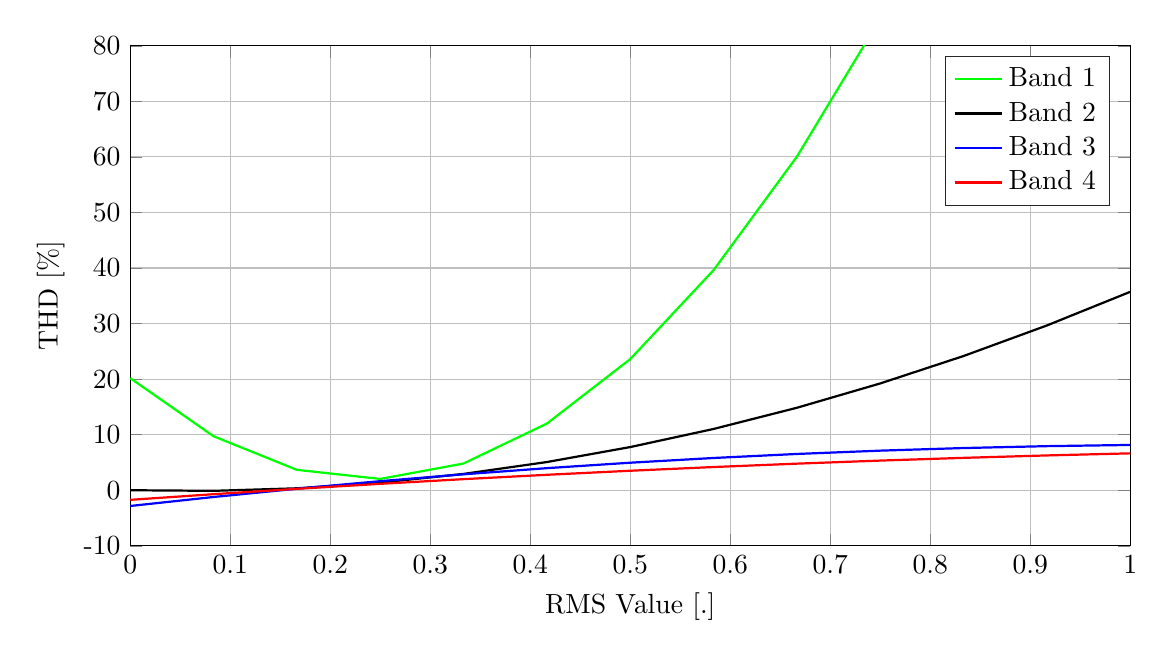
\begin{tikzpicture}

\begin{axis}[%
width=5.0in,
height=2.5in,
at={(0.758in,0.481in)},
scale only axis,
xmin=0,
xmax=1,
xmajorgrids,
ymajorgrids,
xlabel={RMS Value [.]},
ymin=-0.1,
ymax=0.8,
ylabel={THD [\%]},
ytick={-0.1, 0, 0.1,  0.2,  0.3, 0.4, 0.5, 0.6, 0.7, 0.8},
yticklabels={-10,0,10,20,30,40,50,60,70,80},
axis background/.style={fill=white},
legend style={legend cell align=left,align=left,draw=white!15!black}
%every axis legend/.code={\let\addlegendentry\relax}
]
\addplot [color=green,solid,thick]
  table[row sep=crcr]{%
0	0.2018\\
0.0833333333333333	0.0971958333333334\\
0.166666666666667	0.0367166666666667\\
0.25	0.0203625\\
0.333333333333333	0.0481333333333334\\
0.416666666666667	0.120029166666667\\
0.5	0.23605\\
0.583333333333333	0.396195833333334\\
0.666666666666667	0.600466666666667\\
0.75	0.8488625\\
0.833333333333333	1.14138333333333\\
0.916666666666667	1.47802916666667\\
1	1.8588\\
};
\addlegendentry{Band 1};


\addplot [color=black,solid,thick]
  table[row sep=crcr]{%
0	0\\
0.0833333333333333	-0.00105625\\
0.166666666666667	0.00349166666666667\\
0.25	0.01364375\\
0.333333333333333	0.0294\\
0.416666666666667	0.0507604166666667\\
0.5	0.077725\\
0.583333333333333	0.11029375\\
0.666666666666667	0.148466666666667\\
0.75	0.19224375\\
0.833333333333333	0.241625\\
0.916666666666667	0.296610416666667\\
1	0.3572\\
};
\addlegendentry{Band 2};

\addplot [color=blue,solid,thick]
  table[row sep=crcr]{%
0	-0.02834\\
0.0833333333333333	-0.0121695138888889\\
0.166666666666667	0.00272527777777777\\
0.25	0.016344375\\
0.333333333333333	0.0286877777777778\\
0.416666666666667	0.0397554861111111\\
0.5	0.0495475\\
0.583333333333333	0.0580638194444444\\
0.666666666666667	0.0653044444444444\\
0.75	0.071269375\\
0.833333333333333	0.0759586111111111\\
0.916666666666667	0.0793721527777778\\
1	0.08151\\
};
\addlegendentry{Band 3};

\addplot [color=red,solid,thick]
  table[row sep=crcr]{%
0	-0.01729\\
0.0833333333333333	-0.00709902777777778\\
0.166666666666667	0.00250722222222222\\
0.25	0.01152875\\
0.333333333333333	0.0199655555555556\\
0.416666666666667	0.0278176388888889\\
0.5	0.035085\\
0.583333333333333	0.0417676388888889\\
0.666666666666667	0.0478655555555556\\
0.75	0.05337875\\
0.833333333333333	0.0583072222222222\\
0.916666666666667	0.0626509722222222\\
1	0.06641\\
};
\addlegendentry{Band 4};

\end{axis}
\end{tikzpicture}
    \caption{4 Interpolated model describing the worst case THD in each band.}
    \label{fig:CombinedModel}
\end{figure}






\section{Error sources}
Few errors could have occurred during trials, since then only variable adjusted during between measurements were the gain of the amplifier. There were however problems with moving the setup from the control room were it was calibrated and then moved into the anechoic room. The
calibration was done using an visual equalizer where the output was shown with a bar chart. Hence the data should bee seen with a tolerance of +/- 0.5 dB.

\section{Conclusion}

